\documentclass[a4paper]{book}

\usepackage[paperwidth=169mm, paperheight=239mm]{geometry}

%\usepackage[latin9]{inputenc}
\usepackage[utf8x]{inputenc}
\usepackage[pdftex]{graphicx}
\usepackage{pdfpages}
\usepackage[british]{babel}
\usepackage{placeins}
\usepackage{dialogue}
\usepackage{fancyvrb}

\usepackage{t1enc}         
\usepackage{times}
\usepackage{url}
\usepackage{enumerate}

%\usepackage{code}
\usepackage{hyperref}
\usepackage{amsmath}
\usepackage{amssymb}
\usepackage{mathtools}
%\usepackage{lingmacros}
\usepackage{subfig}
\usepackage{fancyhdr}


\pagestyle{plain}
%\pagenumbering{arabic}


%stuff
\usepackage{latexsym}
\usepackage{tikz,pgflibraryshapes}
\usetikzlibrary{shapes,snakes,positioning,matrix}
\usepackage{pgfplots}
\usepackage{booktabs}
\usepackage{enumerate}
%\usepackage{etoolbox}


\usepackage{multibib} 
\newcites{bb}{Bibliography} 
\newcites{ifl}{Bibliography}
\newcites{papp}{Bibliography}
\newcites{exp}{Bibliography}
\newcites{hl}{Bibliography}
\newcites{csort}{Bibliography}
\newcites{emb}{Bibliography}
\newcites{arbb}{Bibliography}
\newcites{t}{Bibliography}
%\newcites[ifl}{Bibliography}

%\patchcmd{\thebibliography}{\section*}{\section}{}{}

\makeatletter
\renewenvironment{thebibliography}[1]
     {\section*{\bibname}%
      %\@mkboth{\MakeUppercase\bibname}{\MakeUppercase\bibname}%
      \list{\@biblabel{\@arabic\c@enumiv}}%
           {\settowidth\labelwidth{\@biblabel{#1}}%
            \leftmargin\labelwidth
            \advance\leftmargin\labelsep
            \@openbib@code
            \usecounter{enumiv}%
            \let\p@enumiv\@empty
            \renewcommand\theenumiv{\@arabic\c@enumiv}}%
      \sloppy
      \clubpenalty4000
      \@clubpenalty \clubpenalty
      \widowpenalty4000%
      \sfcode`\.\@m}
     {\def\@noitemerr
       {\@latex@warning{Empty `thebibliography' environment}}%
      \endlist}
\makeatother


%%

%% \newcommand{\bequ}{\begin{quote}}
%% \newcommand{\enqu}{\end{quote}}
%% \newcommand{\eop}[1]{\mbox{\sl #1}}
%% \newcommand{\sube}[2]{#1_{#2}}
%% \newcommand{\id}[1]{{\it #1}}
%% \newcommand{\kwd}[1]    {\mbox{\textbf{#1}}}
%% \newcommand{\str}[1]{{\id "#1"}}
%% \newcommand{\lemon}{\emph{lemon}}
%% \newcommand{\textt}[1]{\texttt{#1}}
%% \newcommand{\txttt}[1]{\texttt{#1}}

%\renewcommand*{\thesection}{\arabic{section}}

\newcommand{\thesistitle}{Embedded Languages for Data-Parallel Programming}
\newcommand{\dept}{Department of Computer Science and Engineering}
\newcommand{\uni}{Chalmers University of Technology and G\"oteborg University}
\newcommand{\group}{Functional Programming Research Group}


% ---------------------------------------------------------------------------
% Papers 
% ---------------------------------------------------------------------------
\newcommand{\paperA}{Paper A}
\newcommand{\paperATitle}{Simple and Compositional Reification of Monadic Embedded Languages}
\newcommand{\paperB}{Paper B}
\newcommand{\paperBTitle}{Obsidian: A Domain Specific Embedded Language for Parallel Programming of Graphics Processors}
\newcommand{\paperC}{Paper C} 
\newcommand{\paperCTitle}{GPGPU Kernel Implementation and Refinement using Obsidian} 
\newcommand{\paperD}{Paper D}
\newcommand{\paperDTitle}{Expressive Array Constructs in an Embedded GPU Kernel Programming Language}
\newcommand{\paperE}{Paper E}
\newcommand{\paperETitle}{Counting and Occurrence Sort for GPUs using an Embedded Language}
\newcommand{\paperF}{Paper F}
\newcommand{\paperFTitle}{A High-Level Embedded Language for Low-Level GPU Kernel Programming}
\newcommand{\paperG}{Paper G}
\newcommand{\paperGTitle}{Programming Future Parallel Architectures with Haskell and Intel ArBB}
\newcommand{\paperH}{Paper H}
\newcommand{\paperHTitle}{Parallel Programming in Haskell Almost for Free}

% ---------------------------------------------------------------------------
% BEGIN ! 
% ---------------------------------------------------------------------------
\begin{document}

\begin{titlepage}
\begin{centering}
{\sc Thesis for the Degree of Doctor of Philosophy}
\vspace{30ex}

{\LARGE\bf\thesistitle}

\vspace{7ex}

\large Bo Joel Svensson
\vfill

\includegraphics[width=120mm]{./img/ChalmGUtextsvEng}\\[5mm]

\includegraphics[height=4cm]{./img/ChalmGUmarke}\\

\vspace{1cm}
\normalsize
{\sc \dept}\\
{\sc \uni}\\
G\"oteborg, Sweden 2013

\end{centering}
\end{titlepage}

% ---------------------------------------------------------------------------
% Tryckortssida
% ---------------------------------------------------------------------------
%ditt ISBN är:  978-91-7385-939-4
%ditt Ny serie nr:  3620
%ISSN för publ.serien Doktorsavhandlingar vid Chalmers tekniska högskola : 0346-718X

\quad \vfill

{\noindent\large\bf\thesistitle} \\
\noindent Bo Joel Svensson \\
\noindent ISBN 978-91-7385-939-4 \\

\vspace{1cm}

\noindent\copyright {\sc {Bo Joel Svensson}}, 2013 \\ 
\vspace{1cm} 


\noindent Doktorsavhandlingar vid Chalmers tekniska högskola \\
\noindent Ny serie nr 3620 \\
\noindent ISSN 0346-718X \\

\vspace{1cm}

\noindent Technical Report 101D\\
\noindent \dept \\
\noindent \group\\

\vspace{1cm} 

\noindent \uni \\
\noindent SE--412~96~~G\"oteborg, Sweden\\
\noindent Phone: +46 (0)31--772~1000 \\

\vspace{1cm} 

\noindent Printed in Sweden\\
\noindent Chalmers Reproservice\\
\noindent G\"oteborg, Sweden 2013


\thispagestyle{empty}

\clearpage
\pagenumbering{roman}

% ---------------------------------------------------------------------------
% ABSTRACT !!  
% ---------------------------------------------------------------------------
\section*{Abstract}

Computers today are becoming more and more parallel. General purpose processors (CPUs) 
have multiple processing cores and Single Instruction Multiple Data (SIMD) units for 
data-parallelism. Graphics processors (GPUs) bring massive parallelism at the cost of 
being harder to program than CPUs. This thesis applies embedded language methodology 
to data-parallel programming. Two embedded languages are presented, Obsidian for general 
purpose GPU programming and EmbArBB for data-parallel programming across platforms. 

CPUs and GPUs get more parallel resources with each new generation. The question of how to 
efficiently program these processors arises. We are after efficiency both in programmer 
productivity and in application performance. Using embedded languages allows us to experiment
with what abstractions to present to the programmer at relatively little effort.

Obsidian is an embedded language for general purpose programming of GPUs. We try to strike 
a balance between high level, productivity increasing abstractions and low-level 
control needed for performance. The Obsidian programming model mirrors the GPU architecture 
and the programmer is constrained into writing GPU-friendly code. Hierarchy level 
polymorphic library functions are supplied to make these constraints feel less obtrusive. 
Obsidian programs are compiled into CUDA C code. This compilation is based on a simple 
and elegant monad reification technique.  

In cases where the programmer is not interested in low-level details 
or wants the program to run over a range of hardware, a higher level language can be used.
EmbArBB is a Haskell embedding or the Intel ArBB system. EmbArBB relies on the ArBB system 
to generate code (via a Just-In-Time compiler) to a range of hardware. 

EmbArBB embeds a preexisting library for data-parallelism into Haskell and we obtain 
very good performance at little implementation effort. This performance comes from the 
expertise and effort put into the ArBB system and that we get for free. Embedding ArBB is 
a way to provide these benefits to the Haskell programmer and a way to increase usefulness
of an existing system by opening it up to a wider audience. Obsidian is very different; it 
is not based on a set of high-level parallel primitives. The Obsidian programmer 
can implement these primitives in different ways and then select the best one. 
We have obtained very good performance in case studies involving reductions. Obsidian 
programs are also more terse and composable, compared to CUDA. 
 
\vspace{5mm}

\noindent

\textbf{Keywords:} Data-parallelism, Embedded languages, Functional Programming, Graphics Processing Units

\clearpage

% ---------------------------------------------------------------------------
%  ACKS !!! 
% ---------------------------------------------------------------------------
\section*{Acknowledgments}

I would like to thank my supervisor Mary Sheeran. She is a very supportive, motivating and 
understanding supervisor. I also thank my co-supervisor Koen Claessen for all the great advice 
and tips he has provided over the years. I cannot imagine that this would have worked with 
any other supervisors. Thanks to Josef Svenningsson, a late addition to my troop of 
supervisors. Working with Josef has been fun and rewarding. 

I have often turned to Emil Axelsson with technical questions, and he has always been
happy to help. For this I am grateful. 

I thank Manuel Chakravarty for letting me visit his group at the University of New South Wales 
and Trevor McDonell and Sean Lee for taking care of me during my visit. I look back 
very fondly to my stay in Australia. 

For being a great supervisor during my three month internship at Intel, I thank Ryan Newton. 
These where three very intense months away from family but at the same time a very rewarding 
experience. 

Thanks to my thesis opponent Stephen Edwards for valuable comments on a draft of this thesis. 

I want to thank Erik, Ola, Markus and Viktor for our occasional lunches and GPU discussions. 
I also thank my office mates, Michal and Nicholas, for their company. I thank Eva Axelsson, 
who I have felt most comfortable to turn to for help and information, even when she was not 
the appropriate channel. 

Finally I want to thank my family and friends. Thanks to my sisters and parents for their support.
I thank my friends for being understanding during times when I have been very self-absorbed. 
I am very grateful to my wife Andrea for supporting and believing in me and to our daughter Noemi 
for bringing much joy to my breaks from work while writing this thesis; soon she is old enough 
for real LEGO. 

\vspace{5mm}
\noindent This research has been funded by the Swedish Foundation for
Strategic Research (which funds the Resource Aware Functional 
Programming (RAW FP) Project) and by the Swedish Research Council.

\clearpage

% ---------------------------------------------------------------------------
%  Guide for Opponent, grading committee
% ---------------------------------------------------------------------------
\section*{Publications}

This thesis includes the following publications: 

\begin{enumerate}[A.] 
\item Josef Svenningsson and Bo Joel Svensson. Simple and Compositional Reification of Monadic Embedded Languages, 2013. \emph{18th ACM SIGPLAN International Conference of Functional Programming, ICFP 2013.}
\item Bo Joel Svensson, Mary Sheeran and Koen Claessen. Obsidian: A Domain Specific Embedded Language for General Purpose Parallel Programming of Graphics Processors. In \emph{Proc. of Implementation and Applications of Functional Languages (IFL)}, Lecture Notes in Computer Science, Springer Verlag, March 2009.
\item Bo Joel Svensson, Koen Claessen and Mary Sheeran. GPGPU kernel implementation and refinement using Obsidian. \emph{Practical Aspects of High-level Parallel Programming, PaPP 2010.} Procedia Computer Science.
\item Koen Claessen, Mary Sheeran and Bo Joel Svensson. Expressive Array Constructs in an Embedded GPU Kernel Programming Language. In \emph{Proceedings of the 7th workshop on Declarative aspects and applications of multicore programming}, DAMP '12. ACM. 
\item Josef Svenningsson, Bo Joel Svensson and Mary Sheeran. Efficient Counting Sort Implementations using an Embedded GPU Programming Language. \emph{2nd Workshop on Functional High-Performance Computing, FHPC '13.}
\item Bo Joel Svensson and Mary Sheeran. A High-Level Embedded Language for Low-Level GPU Kernel Programming. {\bf\emph{This work has not yet been published.}} 
\item Bo Joel Svensson and Ryan Newton. Programming Future Parallel Architectures with Haskell and ArBB. \emph{Future Architectural Support for Parallel Programming (FASPP), in conjunction with ISCA '11.}
\item Bo Joel Svensson and Mary Sheeran. Parallel Programming in Haskell Almost for Free: an embedding of Intel's Array Building Blocks. \emph{Proceedings of the 1st ACM SIGPLAN Workshop on Functional High-Performance computing, FHPC '12.}
\end{enumerate} 

\clearpage
\subsection*{Personal contributions} 

The following describes my personal contributions to the papers included 
in this thesis. 

\subsubsection{Paper A}
I intuitively applied the monad reification method as part of the implementation 
of Obsidian. Josef Svenningsson identified its importance and suggested we write 
about it. The paper has two distinct parts. Sections one and two describe the 
method as I used it. And section four makes the compositional aspect of the method 
explicit. 

The code and examples in section one and two are my work. The contents of section four was 
developed by Josef Svenningsson and me. For section four we also got very much and valuable help 
from Emil Axelsson. 

For the rest of the paper, just substituting my name for Benny and Josef's for Bj\"orn
will give a good indication of our contributions. 

\subsubsection{Papers B, C, D and E} 
The Obsidian language has grown out of discussions between Mary Sheeran, Koen Claessen and me. 
When it comes to implementation of the ideas we had in these discussions, I have been responsible. 
Push arrays, first appearing in paper D, were invented by Koen Claessen. However, the 
implementation of them in the setting of Obsidian was done by me. Paper D also has large 
contributions by Mary Sheeran when it comes to examples and implementing them. 

Paper E was the first I wrote with Josef Svenningsson, who had been thinking about an interesting
variation of counting sort and wanted to implement it. Together we added atomic operations to 
Obsidian and I modified the code generator to accommodate them. Sections 
1 and 2 in the paper are written by Josef. Sections 3 through 7 are mostly my work, including 
the benchmarking. Section 8 is joint work.
%Me and Josef are equal partners in this paper and got much valuable advice from 
%Mary Sheeran. 

\subsubsection{Papers G and H} 
The work behind paper G, work was performed by me 
under supervision of Ryan R. Newton who is also mostly responsible for the writing of the 
paper. Programming and running time experimentation was performed by me, while getting much 
valuable advice and guidance from Ryan. 

The work behind paper H was done by me as a hobby project and my aspirations were not 
high. I just wanted to experiment with some embedded language techniques that we had 
been avoiding (had no need for) in Obsidian. Mary discovered what I was doing and applied 
the right amount of pressure, leading to us encompassing much more of ArBB functionality than 
I had in mind. The paper's text is joint work; most examples as well as benchmarking are my work,
but the sparse matrix vector multiplication example is entirely Mary's. 

%Intel has unfortunately retired the ArBB project. This leaves EmbArBB without a functioning 
%code generating backend u

% \subsection*{Guide} 

\tableofcontents


\cleardoublepage
\clearpage

\pagenumbering{arabic}
\pagestyle{fancy}
\fancyfoot{}
\fancyhead[LO]{}
\fancyhead[RO]{\leftmark}
\renewcommand{\headrulewidth}{0.0pt}
\fancyhead[LE,RO]{\thepage}

% --------------------------------------------------------------------------- %
% --------------------------------------------------------------------------- %
%
%  INTRODUCTION 
%
% --------------------------------------------------------------------------- %
% --------------------------------------------------------------------------- %
\chapter{\thesistitle}

% -------------------------------------------------------------------------
%  INTRO SECTION OF INTRO CHAPTER
% -------------------------------------------------------------------------

\section{Introduction} 

This thesis applies embedded language methodology to data-parallel programming of 
massively parallel hardware. An embedded language is a language that is implemented 
as a library for some existing host language. In this case, the functional programming 
language Haskell is used as host language. 

Computers today are increasingly parallel. Each new generation of general purpose processors
(CPUs) and of graphics processors (GPUs) brings more parallelism. The question 
of how to program these computers most efficiently, both from a productivity and 
a performance point of view, arises. Explicit parallel programming is hard and automatic 
means of parallelisation, while giving a sequential programming model to the programmer, 
often misses the target when it comes to performance. The book ``Structured Parallel 
Programming'' by Michael McCool et al argues the need for explicit parallel programming 
models~\citet{STRUCTURED}.

The embedded language approach to programming language implementation is beneficial, 
since we are not entirely sure of how to program current and future highly parallel 
computers. Implementing an embedded language allows us more rapid prototyping of ideas. 
We can experiment with what abstractions to expose to the programmer, without much 
effort. There are many other benefits of embedded languages: making use 
of the host language's library functions (if they are general enough), the host language 
can be used as a powerful macro language for the embedded language, providing a more 
leveled learning curve to programmers already familiar with the host language. 
For programmers who are already proficient in the host language, learning an embedded 
language is more like picking up a new library. 

This thesis focuses on data-parallelism, as opposed to task or control parallelism.
Data-parallelism is applicable where the input data can be divided into chunks
and operated upon independently. Data-parallelism is scalable; the potential 
for parallelism increases with the problem size. Two different embedded languages 
for data-parallel programming are presented in this thesis: Obsidian, for 
general purpose computations on GPUs and EmbArBB for parallel programming across 
platforms, such as CPUs, GPUs and other accelerators. 

Graphics Processors trade programmer convenience for increased parallelism. 
For example, where CPUs dedicate large portions of chip area to caches, branch 
prediction and instruction level parallelism (ILP), GPUs put additional cores. 
This comes at a price of increased programmer effort. GPUs have programmer managed 
shared memories, conditionals are troublesome from a performance 
perspective and memory access patterns can make or break the performance of an 
application. With Obsidian, we try to find the right level of abstraction for 
programming GPUs. We try to strike a balance between low-level control of details 
that influence performance and high-level abstractions to increase productivity and 
make programs more terse. The end goal with Obsidian is a language for writing 
high performance GPU programs that compare well to code written by CUDA~\citet{CUDA}  
(a C-dialect for GPU programming) experts, provided that both programmers have 
similar GPU expertise. The Obsidian programmer would however write programs in a more 
composable manner. Obsidian programs are compiled into CUDA.  

Obsidian is geared towards the programmer who is interested in GPU hardware. Making 
good use of Obsidian requires that the programmer is willing to make an effort 
to learn about GPUs and how to program them efficiently. However, another case 
is a programmer who does not want to invest that effort but wants to write a high-level 
parallel program and have it run reasonably well on different parallel architectures. 
In this case, a language with even higher level of abstraction is preferable. It then 
becomes the job of a more advanced compiler to turn that into code for the targeted 
platforms. The EmbArBB language targets this programmer. EmbArBB exposes a set of high-level 
operations on arrays, such as {\tt map}, {\tt reduce} and {\tt scan}. The programmer 
has no power over the parallel strategy that should be used to implement these 
operations but instead relies on a JIT-compiler (Just In Time-compiler). EmbArBB is a 
Haskell embedding of Intel ArBB~\citet{ARBB2011} that was released as an embedded language 
in C++. EmbArBB relies entirely on the ArBB system for code generation and optimisation.  

% -------------------------------------------------------------------------
% Obsidian !
% -------------------------------------------------------------------------

\section {Obsidian: An embedded language for GPU kernel implementation} 

In 2006, NVIDIA released their first Compute Unified Device Architecture (CUDA) 
GPU. With CUDA, NVIDIA also made it a lot easier for programmers to use GPUs
for general purpose programming~\citet{wwwcuda}. A dialect of C, called CUDA C, was released 
specifically to simplify the implementation of general purpose computations on GPUs. 

Before CUDA, programmers still tried (very ingeniously) to make use of GPUs for 
non-graphics applications via the graphics API. The desired computation was expressed 
in graphics terms and the result computed through an act of rendering. Of course, since the 
available abstractions targeted the graphics domain, this added extra
burden on the programmer. CUDA was NVIDIA's first response to this problem. CUDA 
is a dialect of C, extended with a parallel programming model suitable for GPUs. 

Having a language specifically made for general purpose programming on the GPU, such as 
CUDA, is a big step up from earlier. But CUDA still offers a very low-level interface to 
programming the GPU, which is preferred in a situation where the programmer needs to 
think about hardware specific details to get the best performance. CUDA provides this, 
but at the price that it is hard to build upon, abstract and reuse prior programming 
effort. This is where we are trying to go one step further with Obsidian. 

% -------------------------------------------------------------------------
% GPU Hardware 
% -------------------------------------------------------------------------

\subsection{GPU hardware} 

Before going into programming of GPUs, it is important to have some background. The 
GPU programming model exposed by CUDA very much mirrors the underlying hardware. Some 
of the details that make GPU programming hard are more apparent when looking at the 
underlying hardware. 

A CUDA GPU is built around a single kind of processor (as opposed to the different 
kinds of processors found in earlier GPUs). The processors in the GPU (called MPs, 
MultiProcessors) all contain a number of cores called SPs (Streaming Processors). 
Each MP also contains local memory, called shared memory since it can be accessed 
by all of the SPs in that MP. The number of MPs varies over the available GPUs; cheaper 
GPUs have as few as one MP, and as you go up in price the number of MPs increases.

Each MP of the GPU can manage a large number of threads; on today's GPUs up to 
2048 threads can run on a single MP. The GPU schedules threads in groups of 32, called 
{\em Warps}, that are executed in lock-step (SIMD style execution). Threads are 
also divided into {\em Blocks}; the threads within a block can communicate using the 
shared memory. The maximum block size is currently 1024 threads. Threads within 
a warp can communicate via the shared memory without using any synchronisation 
primitive. However, if communication takes place across warps synchronisation is 
necessary. A barrier synchronisation mechanism exists to ensure that all threads within a block 
have reached the same position in the code. Blocks are also grouped into a grid that 
is the collection of blocks executing the same program. 

% -------------------------------------------------------------------------
%  GPU Programming
% -------------------------------------------------------------------------

\subsection{GPU programming} 
\label{sec:GPUPROGRAMMING}

The CUDA programming model reflects the hierarchical architecture of the GPU. The 
programmer writes what are called \emph{kernels}; in CUDA jargon, a kernel refers to a sequential 
C program that is parameterised on a thread's identity. The kernel program is executed 
in parallel across all the threads of a block and many such blocks of threads can execute 
in parallel on the available MPs. Kernels may use shared memory that is local to a block; 
the programmer needs to decompose the algorithm and data in such a way that communication 
will be local to the blocks. 


The program below is a very simple example of a CUDA kernel that computes elementwise sums. 

\begin{small}
\begin{Verbatim}[samepage=true]
__global__ void vecAdd(int32_t *i1, int32_t *i2, int32_t *r) {
  
  unsigned int gid = blockIdx.x * 
                     blockDim.x + 
                     threadIdx.x;

  r[gid] = i1[gid] + i2[gid]; 

} 

\end{Verbatim}
\end{small}

\noindent The kernel takes two input arrays, {\tt i1} and {\tt i2}; the result is stored 
in {\tt r}. Note how the kernel makes use of three variables, {\tt threadIdx.x}, 
{\tt blockIdx.x} and {\tt gridDim.x}. These variables identify a thread uniquely within 
a grid. Here they are used to obtain an index into the provided arrays. The dimensions of 
the blocks and of the grid are set by a controlling program upon launch of the kernel. This 
controlling program is run by the CPU of the computer housing the GPU. The kernel is launched 
using the following syntax: 

\begin{small} 
\begin{Verbatim}[samepage=true]
vecAdd<<<1,32,0>>>(d_i1,d_i2,d_r);
\end{Verbatim}
\end{small}

\noindent This line of code launches the kernel on one block of 32 threads. The zero 
indicates that the kernel uses no shared memory. If the kernel did use shared memory, the 
amount needed should have been specified there. Figure~\ref{fig:CUDACODE1} shows the complete 
sequence of commands for a minimal example using the kernel specified above. 

% -------------------------------------------------------------------------
% CUDACODE1 FIGURE
% -------------------------------------------------------------------------

\begin{figure} 
\begin{small}
\begin{Verbatim}[samepage=true]
int main(void) {
  
  int32_t h_i1[32], h_i2[32], h_r[32]; 

  int32_t *d_i1, *d_i2, *d_r;

  
  for (int i = 0; i < 32; ++i) { 
    h_i1[i] = i;
    h_i2[i] = 32 - i;
  }

  // Allocate device memory
  cudaMalloc((void**)&d_i1,32*sizeof(int32_t));
  cudaMalloc((void**)&d_i2,32*sizeof(int32_t));
  cudaMalloc((void**)&d_r,32*sizeof(int32_t));
  
  // Copy inputs to device
  cudaMemcpy(d_i1,
             h_i1,
             32*sizeof(int32_t),
             cudaMemcpyHostToDevice);
  cudaMemcpy(d_i2,
             h_i2,
             32*sizeof(int32_t),
             cudaMemcpyHostToDevice);
  
  // Launch the kernel
  vecAdd<<<1,32,0>>>(d_i1,d_i2,d_r); 

  // Copy result to host
  cudaMemcpy(h_r,
             d_r,
             32*sizeof(int32_t),
             cudaMemcpyDeviceToHost);

  for (int i = 0; i < 32; ++i) { 
    printf("%d ",h_r[i]);
  }

  return 0;
}
\end{Verbatim} 
\end{small}

\caption{Host code for launching a simple CUDA kernel on the GPU.}
\label{fig:CUDACODE1}

\end{figure} 

% -------------------------------------------------------------------------
% 
% -------------------------------------------------------------------------

\noindent In Obsidian, the same kernel (the local computation) is implemented as follows: 

\begin{small}
\begin{Verbatim}[samepage=true]
vecAdd :: Num a => SPull a -> SPull a -> SPull a
vecAdd = zipWith (+)
\end{Verbatim}
\end{small}

\noindent The {\tt vecAdd} program takes two {\tt SPull} input arrays and gives one 
as result. The Obsidian {\tt vecAdd} is more general than the CUDA version. From it 
we can generate CUDA kernels for any element type that supports the {\tt (+)} operation. 
In Haskell we know that types that belong to the {\tt Num} type class has a {\tt (+)} operation.  

There are some important differences between CUDA and Obsidian programs. One is that with Obsidian 
we generate kernels for fixed size local computations. This is to avoid doing out-of-bounds checks 
which would mean conditionals in the code. Conditionals are problematic from a performance 
point of view. Another difference is that in Obsidian the programmer specifies the entire 
computation, including how it is mapped over the blocks of the GPU. This is done implicitly 
in CUDA, based on the indexing arithmetic used in the kernel and the number of blocks and 
threads provided at kernel launch. This means that the Obsidian programmer needs to 
write a program that performs this mapping: 

\begin{small} 
\begin{Verbatim}[samepage=true]
vecAddG :: Num a => DPull a -> DPull a -> DPush Grid a
vecAddG i1 i2  =
  pConcat $
  fmap push $ 
  zipWith vecAdd
          (splitUp 32 i1)
          (splitUp 32 i2)  
\end{Verbatim}
\end{small} 

The {\tt vecAddG} program specifies a computation on large arrays; the large input arrays 
are split up into pieces that are operated upon by the local computation, {\tt vecAdd}, 
specified above. Each input array passed to this function must have length a multiple of 32.
Since the {\tt splitUp} operation splits the arrays into chunks of 32 elements, the body 
of the generated kernel will be constructed specifically for this size. {\tt zipWith} is 
used to map the local computation onto each chunk of the input arrays. The result is an 
array of arrays that is flattened with the {\tt pConcat} function. The CUDA code below 
is generated from the {\tt vecAddG} program: 

\begin{small}
\begin{Verbatim}[samepage=true] 
extern "C" __global__ void vecAdd(int32_t* input0, uint32_t n0,
                                  int32_t* input1, uint32_t n1,
                                  int32_t* output2)
{
    uint32_t tid = threadIdx.x;
    
    if (blockIdx.x < min(n0 / 32U, n1 / 32U)) {
        output2[blockIdx.x * 32U + tid] = 
            input0[blockIdx.x * 32U + tid] +
            input1[blockIdx.x * 32U + tid];
    }
}
\end{Verbatim}
\end{small} 

There are some superficial differences between the code generated using Obsidian and the 
handwritten example above. One such difference is that the index computation is not shared. 
Obsidian relies on the CUDA compiler to discover such sharing via a Common Subexpression 
Elimination (CSE) optimisation pass. Another difference is that Obsidian has inserted a 
conditional that only executes the body for certain blocks. Discussion of the causes for 
that conditional is postponed until section~\ref{sec:OBSARRAYS}. A real 
difference is that the kernel is generated for a fixed size; here there is a constant (32) 
where in the handwritten code we used {\tt blockDim.x}. If those differences are set 
aside, the two kernels are identical. Figure~\ref{fig:OBSIDIANHOST1} shows how the 
{\tt vecAddG} kernel can be launched from within Haskell, using Obsidian's rudimentary 
support for launching GPU computations. 

An alternative way to implement {\tt vecAddG} is to inline the local computation 
directly. This makes the entire program look like this. 

\begin{small}
\begin{Verbatim}[samepage=true]
vecAddG :: Num a => DPull a -> DPull a -> DPush Grid a
vecAddG i1 i2  =
  pConcat $
  fmap push $
  zipWith (zipWith (+)) 
          (splitUp 32 i1)
          (splitUp 32 i2)
\end{Verbatim} 
\end{small} 

\noindent The generated code looks exactly as before. 

% -------------------------------------------------------------------------
% OBSIDIANHOST1 FIGURE
% -------------------------------------------------------------------------

\begin{figure} 
\begin{small}
\begin{Verbatim}[samepage=true]
performVecAdd =
  withCUDA $
  do
    kern <- capture 32 (vecAddG :: DPull EInt32
                                 -> DPull EInt32
                                 -> DPush Grid EInt32)

    useVector (V.fromList [0..32::Int32]) $ \i1 ->
      useVector (V.fromList [0..32::Int32]) $ \i2 -> 
        allocaVector 32 $ \(o :: CUDAVector Int32) ->
        do
          fill o 0
          o <== (1,kern) <> i1 <> i2 

          r <- peekCUDAVector o
          lift $ putStrLn $ show r
\end{Verbatim} 
\end{small}

\caption{Host code for launching a simple Obsidian kernel on the GPU. \\ 
 {\tt capture} compiles an Obsidian program into CUDA. At this point the 
  types of the Obsidian program need to be made concrete. The number, 32, used as 
 an argument to {\tt capture} specifies that generated code should be specialised 
 for 32 threads per block. }
\label{fig:OBSIDIANHOST1}
\end{figure} 

\pagebreak 

\noindent A CUDA kernel that uses shared memory takes the form: 

\begin{small}
\begin{Verbatim}[samepage=true]
__global__ void kernel(int32_t *i, int32_t *r) {

  extern __shared__ int32_t sm[]; 

  unsigned int tid = threadIdx.x; 
  unsigned int gid = blockIdx.x * 
                     blockDim.x + 
                     threadIdx.x;

  sm[tid] = i[gid]; 
  __syncthreads();

  /* Compute on sm */ 
     
  __syncthreads();
  r[gid] = sm[tid]; 
  
}
\end{Verbatim} 
\end{small} 

\noindent A portion of the input array is stored into shared memory. A 
barrier synchronisation is used to ensure that each thread within the block 
has stored its value into shared memory (only necessary if threads will 
communicate across warp boundaries). After computing on the data locally, 
it is written back into global memory. This kernel sets up two aliases for 
thread identities. A thread's global identity is called {\tt gid} and its local 
identity is called {\tt tid}. The global ID is used to index into the large global 
array; indexing into local shared memory is done using the local ID. 

In Obsidian, local computations can also use shared memory. The Obsidian arrays 
we have seen in the examples, {\tt Pull} and {\tt Push} arrays do not directly 
correspond to actual data in memory. Pull and push arrays rather represent ways 
to compute arrays. More information about these array representations is available 
in section~\ref{sec:OBSARRAYS}. The Obsidian programmer can store intermediate 
arrays in shared memory by using a {\tt force} operation. 
%The 
%{\tt force} operation computes an array and stores it into shared memory. 

The following kernel multiplies each element in an array by two and then adds one: 

\begin{small}
\begin{Verbatim}[samepage=true] 
kernel :: Num a => SPull a -> SPull a
kernel = fmap (+1) . fmap (*2)
\end{Verbatim}
\end{small}

\noindent This kernel computes its result without any storage of intermediate results;
the code is equivalent to \verb!fmap ((+1).(*2))!. 
In the generated CUDA code below, it can be seen that the (*2) and (+1) operations 
are applied without any intermediate storage. 

\begin{small}
\begin{Verbatim}[samepage=true]
extern "C" __global__ void kernel(int32_t* input0, uint32_t n0,
                                  int32_t* output1)
{
    uint32_t tid = threadIdx.x;
    
    if (blockIdx.x < n0 / 32U) {
        output1[blockIdx.x * 32U + tid] = 
          input0[blockIdx.x * 32U + tid] * 2 + 1;
    }
}
\end{Verbatim}
\end{small}

Storing an intermediate result between the two operations can be accomplished by 
changing the kernel as follows. 

\begin{small}
\begin{Verbatim}[samepage=true]
kernelF :: (MemoryOps a, Num a)
         => SPull a -> BProgram (SPull a)
kernelF = liftM (fmap (+1)) . force . fmap (*2)
\end{Verbatim} 
\end{small} 

This change introduced some noise. The reason for this is that Obsidian programs that 
use memory are monadic. The {\tt BProgram} in the result type is a monad. Another difference 
is that we need to be able to write the array elements to memory; in Obsidian this means 
that the element type must be in the {\tt MemoryOps} class. 

The code below is generated using the {\tt kernelF} program: 

\begin{small} 
\begin{Verbatim}[samepage=true]
extern "C" __global__ void kernel(int32_t* input0, uint32_t n0,
                                  int32_t* output1)
{
    extern __shared__ uint8_t sbase[];
    uint32_t tid = threadIdx.x;
    
    if (blockIdx.x < n0 / 32U) {
        ((int32_t*) sbase)[tid] = 
           input0[blockIdx.x * 32U + tid] * 2;
        __syncthreads();
        output1[blockIdx.x * 32U + tid] = 
           ((int32_t*) sbase)[tid] + 1;
    }
}
\end{Verbatim}
\end{small} 

\noindent This code uses a shared memory array called {\tt sbase}. There 
is also a call to \\ {\tt \_\_syncthreads} to ensure that all the writes have 
completed before proceeding. In this case the synchronisation is not really
necessary since all threads belong to the same warp. There is an {\tt unsafeforce} 
operation that naively removes synchronisations if the array being forced is short 
enough. More advanced analysis could also be performed to remove synchronisations 
whenever communication is entirely warp local. We do not apply that optimisation, 
but work on warp level computations is in progress and would put this ability 
in the hands of the programmer.  

\FloatBarrier 
\subsection{Writing efficient GPU Kernels} 
\label{sec:efficient}
 
Writing efficient GPU kernels is hard. There are many details that the CUDA 
programmer must be aware of in order to make optimal use of the GPU. 
The NVIDIA ``CUDA C Best Practices Guide''~\citet{BestPrac}, is a good source 
to learn more about these details. Here is a list, with explanations of some 
of the practices that the guide deems most important. The list also contains 
information about how these best practices influence our work on Obsidian.  
  
\begin{itemize} 

\item {\bf Minimise data transfers between host and device:} The bandwidth between device memory 
and GPU is much higher than the bandwidth between host memory and the GPU device via the PCIe bus.
This means that, first of all, one must evaluate if the computation to be performed is significant 
enough to warrant a transfer to the GPU. If the computation is not arithmetic intensive, it may be 
better to do the work on the CPU. However, if the data is already in device memory and 
the operation that is about to be performed on it is more efficiently handled by the CPU, it 
may still be better to let the GPU do the work. In other words, compute near the data unless 
transferring it pays off. 

Data transfers between the host memory and device (GPU) memory is out of Obsidian's scope. 
If Obsidian is used to generate kernels for a computation, the programmer has already decided that 
a GPU should be used. However, even after making the decision to use the GPU the programmer 
may need to consider how to transfer the data. In some cases it is possible to overlap 
computation on the GPU and data transfer. These kinds of optimisations are considered 
when writing the C program that launches the CUDA kernels. Obsidian does have rudimentary 
support for launching kernels from within Haskell but currently we consider this mostly a
tool for quickly being able to run a kernel and see what it does, not as a means to implement 
applications. This part of Obsidian is future work. 

\item {\bf Ensure that global memory accesses are coalesced:} Certain access patterns into 
GPU device memory can be {\em coalesced} (combined into few memory transactions). Unfortunately 
what these access patterns are varies somewhat depending on the GPU. For a typical model of 
GPU, the rule is that concurrent memory accesses (by threads within a warp) will be coalesced 
to as many transactions as cache lines touched (128 Byte l1 cache lines). This means that strided 
accesses from within a warp are not favoured. 

Inputs to an Obsidian program are pull arrays. Pull arrays can be arbitrarily permuted; 
the permutation used will decide the access pattern. In section~\ref{sec:OBSARRAYS}, there 
is more information about pull arrays. If global memory accesses can 
be coalesced or not partly also depends on the algorithm being implemented. The next paragraph 
suggests a trick for coalescing memory accesses, in some cases, even if the algorithm is 
unsuitable. Then it becomes a trade between bad memory access pattern and using more 
shared memory. 

\item {\bf Minimise use of global memory:} Accessing global device memory can take as 
many as 400 to 600 clock cycles if the data is not cached, this is 10 - 20 times as many cycles 
as an access to shared memory. The programmer should use shared memory as much as possible 
to avoid redundant loading from global memory. Shared memory can also be used to coalesce 
reads from global memory. Shared memory is a limited resource in the MP, so if a kernel 
uses very much shared memory, fewer such blocks can be active on the MP. 

Intermediate arrays are stored into shared memory when the Obsidian programmer uses 
the {\tt force} function. 

\item {\bf Use a multiple of 32 threads per block:} Groups of 32 threads, warps, are the 
scheduled unit on a GPU. If a warp accesses memory (and will be waiting for it arrive during 
600 cycles) it will be swapped out and another warp will take its place. This means that 
the number of available warps decides how well memory latency can be hidden. A block that is 
not a multiple of 32 leads to wasting GPU resources; some processing elements will stand 
idle during the execution of the incomplete warps. 

Obsidian requires regularity even more than CUDA does. Since we focus on generating high 
performance kernels, we rule out generation of kernels that work on different sizes (per block). 
The choice of how many threads to use per block is in the hands of the Obsidian programmer.
The method for making that choice has changed over time. Earlier, the number of threads 
needed by a kernel was decided by the size of the arrays it computed. This has recently changed
and is now set by a parameter passed to the code generation process.  

\item {\bf Avoid different execution paths within a block:} Any branching instruction that 
causes the execution to branch into different code (in CUDA jargon called a diverging branch) 
within a warp will affect performance. When the execution paths within a warp diverge, the 
computation is serialised. 

Sometimes divergent code cannot be avoided. However, it is important not to have threads 
diverge unnecessarily. When using pull arrays alone, this was often a problem; with the 
addition of push arrays, the situation improved. Using push arrays, some divergent computations 
can be explicitly split up into phases, each phase with all threads following the 
same execution path. This means that fewer threads are required to do the same work. Push arrays 
are explained in more detail in section~\ref{sec:OBSARRAYS}. 

\item {\bf Do not use {\tt \_\_synchthreads()} in diverging code:} Extreme care must be taken 
when synchronising within any conditionally executed code; every thread must reach this barrier.
Failing to ensure this will likely lead to the kernel producing incorrect results. Note that 
this is a major limitation to the composability of CUDA functions. Wheather or not it is safe to 
call some function in a certain place in your code can be decided only by inspecting that 
function's implementation. 

In Obsidian, it is impossible for a barrier synchronisation to appear within diverging 
conditional code. Conditionals can be introduced either by an \\{\tt ifThenElse} function 
at the element level or by a {\tt Cond} statement that is an operation in the {\tt Program} 
monad; we have seen an example of the program monad in section~\ref{sec:GPUPROGRAMMING}. 
The {\tt Program} monad is parameterised on the GPU hierarchy level. There are 
thread programs ({\tt TProgram}), block programs ({\tt BProgram}) and grid programs 
({\tt GProgram}). the {\tt Cond} conditional chooses between two thread programs while a 
synchronisation can only appear in an Obsidian block program. More information about programs 
and the GPU hierarchy is available in section~\ref{sec:OBSIMP}.

%f it is safe or 
%not to call some function at a certain place in your code, can only be decided by inspecting 
%that functions implementation. 
\end{itemize}  

The list above provides some very general guidelines on what to think about when 
writing GPU kernels. The lesson is that fast memory near the processing element 
should be preferred over slow memory far away. Favouring fast memory demands the effort 
of decomposing computation and data in a way that makes this possible. 

% ---------------------------------------------------------------------------
% ---------------------------------------------------------------------------
%
% Obsidian Implementation 
%
% ---------------------------------------------------------------------------
% ---------------------------------------------------------------------------
\subsection{Obsidian Implementation}
\label{sec:OBSIMP}

Obsidian is implemented as an embedded language using Haskell as host. Obsidian 
is a compiled embedded language; a very good paper that is highly relevant to our 
approach is ``Compiling Embedded Languages'' by Conal Elliott et al~\citet{COMPILEEDSL}. 
This paper describes how to embed a compiler backend and generate efficient code 
in some target language. One key aspect of this approach is that the embedded 
language is a library of functions that create and compose Abstract Syntax Trees 
(ASTs). Obsidian (chapter \ref{chap:GPUProgramming}) as well as EmbArBB 
(chapter \ref{chap:ArBB}) are implemented in a similar way. An embedding that builds 
ASTs is called a deep embedding. Shallow embeddings, on the other hand, do not build 
ASTs. In ``Combining Deep and Shallow Embedding for EDSL'' Josef Svenningsson and 
Emil Axelsson combine the two methods, shallow and deep, in order to simplify the 
AST data type (fewer constructors) and make more extensible embedded languages 
\citet{DEEPSHALLOW}. Obsidian also uses a combination of shallow 
and deep embeddings. 

The embedded language approach has become popular to use as a way of raising the 
level of abstraction in fields where the default is to use low-level languages. 
For example, Lava and Wired~\citet{LAVA,Wired} raise the level of abstraction in the 
fields of hardware design and verification and Feldspar does the same in the area of  
digital signal processing~\citet{FELDSPAR2010}. For GPU programming, there are numerous 
embedded approaches using various host languages. Two languages for GPU programming 
embedded in Haskell are  Accelerate and Nikola \citet{ACCELERATEDAMP11, NIKOLA}. 
And there is Intel ArBB, embedded in C++, with the goal of being parallel across 
platforms \citet{ARBB2011}. Related work and information about the tools, libraries 
and languages that make the wider context surrounding Obsidian can be found in 
section~\ref{sec:relatedwork}. 

\subsubsection{Deep embedding: The {\tt Program} data type}

Obsidian uses a deeply embedded {\tt Program} data type that represents GPU Kernels. 
A CUDA GPU has a hierarchy of parallel resources. At the bottom there are threads,  
executing sequential programs. There are groups of threads (of 32) called {\em Warps} that 
execute in lock-step. Warps are the scheduled unit of work on a GPU. There are {\em Blocks} 
of threads, a set of threads that run as a group and share local (shared) memory. And 
lastly there is a {\em Grid} of blocks that specifies the total number of threads involved 
in a computation (Number\_of\_Blocks * Number\_of\_Threads). The deeply embedded program 
data type of Obsidian models this hierarchy by parameterising programs on a hierarchy 
level type parameter (the  {\tt t} parameter below).

\begin{verbatim} 
data Program t a where
\end{verbatim}

The {\tt t} parameter can be either {\tt Thread}, {\tt Warp}, {\tt Block} or {\tt Grid}.
These types are related to each other via a {\tt Step} type constructor that represents 
going upward one step in the hierarchy. 

\begin{verbatim} 
data Step a -- A step in the hierarchy
data Zero
\end{verbatim} 

The {\tt Thread} type is level {\tt Zero} ({\tt type Thread = Zero}). Then {\tt Block} is 
{\tt Step Thread} and {\tt Grid} is {\tt Step Block}. Currently {\tt Warp} is not included 
in the hierarchy, leading to warp programming being a special case. One benefit a warp has is 
that threads can communicate via shared memory without using synchronisation primitives. There 
is no programmer support for warp level programming in CUDA (as there is for block level 
programs). The programmer needs to take care to ensure that the communication patterns are 
within a warp and is then free to remove synchronisations. If warps were to be put in the 
program level hierarchy of Obsidian, its place would be between the thread and block level. 
This would force the programmer to go via warps when putting together a block computation even 
if the communication pattern is not suited for that, leading to inconvenience with no gain. 

As an example of how the hierarchy level parameter is used, I show the {\tt ForAll} constructor 
from the {\tt Program} data type.  This constructor represents parallelism either over threads 
or blocks. 

\begin{verbatim}
ForAll :: EWord32 
            -> (EWord32 -> Program t ())
            -> Program (Step t) ()
\end{verbatim}

{\tt ForAll} takes a number of parallel iterations, and a body represented by a function 
from an index to a program. The body is a {\tt Program} at some level {\tt t} while the 
resulting program is a step above. This means that a thread program can be turned into 
a block program by using {\tt ForAll}, or that a block program can be turned into a grid program. 

Information about the {\tt Program} data type can be found in paper F, \paperFTitle, in 
section \ref{sec:paperF}. 

\subsubsection{Scalars} 

Scalars and operations on scalars are represented by an expression data type \\ ({\tt Exp a}) in 
Obsidian. This is another example of a deep embedding; the expression data type contains 
constructors for literal values, arithmetic operations, and conditionals. 

Haskell's type class system allows us to overload arithmetic operations such as {\tt (+)}, 
{\tt (-)} and {\tt (*)} by making expressions an instance of {\tt Num}. This allows the 
Obsidian arithmetic expressions to look exactly like corresponding native Haskell arithmetic. 

The approach taken to embed the scalar language is very similar to what is described 
in ``Compiling Embedded Languages''~\citet{COMPILEEDSL}; but we use a Generalised Algebraic 
Datatype (GADT) to obtain typed expressions. An alternative to using a GADT is to use phantom 
types, which earlier versions of Obsidian did (section~\ref{sec:paperB}).   


\subsubsection{Arrays} 
\label{sec:OBSARRAYS}

Obsidian has two array representations. These array representations are implemented as 
shallow embeddings on top of the expression and program data types. This means that these 
arrays will disappear during Haskell evaluation of the Obsidian program.
 
\paragraph{Pull arrays:}

Pull arrays have been part of Obsidian from the very beginning~\citet{JMT} but called either 
{\tt Array} or just {\tt Arr}. A pull array represents an array as an indexing function; given 
an index it provides an element: 

\begin{verbatim} 
data Pull s a = Pull {pullLen :: s, 
                      pullFun :: EWord32 -> a}
\end{verbatim} 

Pull arrays are parameterised on both element ({\tt a}) and length ({\tt s}) type. The length 
parameter is used to be able to represent arrays with static (known at Haskell runtime) 
or dynamic (length represented by an expression, an unknown length). When creating block 
level computations, we want to know the exact lengths in order to avoid generating code 
riddled with conditionals concerning array lengths. In CUDA, it is possible to write kernels that 
are not specialised for a certain size. This is accomplished by adding bounds checks. Since 
conditionals  are problematic from a performance point of view, fixed size kernels are recommended 
when performance is crucial. In Obsidian, we have chosen to disallow implementation of kernels 
that operate on different sizes locally.  Dynamic lengths are used for grid level computations; 
this allows a local computation of a fixed size to be run in parallel over arrays a multiple
of the size that the local computation handles. In generated code, this is currently visible 
as a conditional on {\tt blockIdx.x}. However, this is still considered work in progress; the 
conditional is only really necessary for Obsidian kernels that have more than one output array 
and the outputs are of different length. 
%Conditionals are problematic on GPUs and 
%while general programs that run for any size is possible when performance is crucial a fixed 
%size is recommended. 

One benefit of pull arrays is that they give fusion of all operations on them for free. 
For example, {\tt map f} is implemented on pull arrays by composing {\tt f} with the indexing function: 

\begin{verbatim} 
map f (Pull n ixf) = Pull n (f . ixf)
\end{verbatim}

Now, we see that \verb!map f . map g! is the same as \verb!map (f . g)! since both result in {\tt f}
and {\tt g} becoming composed onto the indexing function. No intermediate array is built in 
memory.  

Another benefit of pull arrays is that they are parallel. Simply put, early Obsidian was pull 
arrays in addition to a way to compute the array and store its elements to memory 
(called {\tt sync} in early versions of Obsidian and later {\tt force}). A very 
direct way to compile a pull array to a GPU is to launch as many threads as there are 
elements in the array and apply the indexing function to the thread id. Now each thread 
will have computed an element of the array and can store that to memory. 

 
\paragraph{Push arrays:}

Push arrays were added to Obsidian as a complement to pull arrays. Pull arrays are 
good because they are so simple to understand and easy to parallelise. However, certain
operations on pull arrays yield code that is not suitable for GPU execution. Concatenation 
and interleaving of pull arrays results in conditionals in the indexing function. The 
interleaving case, which is worst, leads to diverging branching in every warp. If branches 
diverge, the GPU turns the processing elements taking one path off and 
allow the others to progress; then turn to the other branch. The computation of the 
branches is serialised and compute resources are wasted. 

Push arrays, like pull arrays, are functions. A Push array is a higher order 
function, taking a function from value and index to a thread program and giving 
as result a program at some level in the hierarchy. The function passed to the 
push array function we call a write-function. Below is the definition of 
push arrays that we use in Obsidian. Push arrays are parameterised on element 
type ({\tt a}), size type ({\tt s}) and program hierarchy level ({\tt p}). 

\begin{verbatim}
data Push p s a =
  Push s ((a -> EWord32 -> TProgram ()) -> Program p ())
\end{verbatim} 

When working with pull arrays, the consumer of such an array decides how to 
iterate over the array and what elements to compute. This is done by applying the 
push array function to those indices that are interesting to the consumer. Push 
arrays work in the opposite way. The Push array (the result program) contains 
the iteration schema; the consumer of the push only decides what write function 
to supply. The iteration schema used is decided upon when creating a push array. 
The code below is an example of how to create a push array from a pull array.

\begin{verbatim} 
convertToPush :: Pull Word32 e 
               -> Push Block Word32 e 
convertToPush (Pull n ixf) =
    Push n $ \wf -> 
      ForAll (fromIntegral n) $ \i -> wf (ixf i) i
\end{verbatim} 

The function above takes a pull array and creates a push array with a parallel 
iteration schema over threads within a block. There are other iteration schemas to 
chose from such as sequential, combinations of sequential and parallel
across both threads and blocks (two level parallelism). 

Push arrays give many of the same benefits as pull arrays. Using push 
arrays, we also get fusion of operations as default. The implementation of map 
(shown below) illustrates how mapping a function {\tt f} over a push array results 
in an application of {\tt f} in the write-function. 

\begin{verbatim} 
map f (Push s p) = Push s $ \wf -> p (\e ix -> wf (f e) ix)
\end{verbatim}

\subsubsection{Compilation to CUDA}

When compiling Obsidian programs to CUDA, we only need to be concerned with the 
{\tt Program} datatype. Given the hierarchy level type parameters to the program datatype, 
we know that the AST can be quite directly translated to CUDA. We know that there will 
be at most one level of nestedness in the parallelism (several blocks, each of several threads). 
This means that we do not need to do any transformations on the AST before generating CUDA code. 
Paper F (section~\ref{sec:paperF}) contains technical details of the compilation process. 

\subsection{Results}
\FloatBarrier 

We have implemented basic algorithms such as sorting, merging, fractal generation, reductions 
and parallel prefix (scans). Often we have managed to get very good performance, close to that 
of hand optimised CUDA code. GPU execution of scan operations is something that has 
been worked on extensively in the GPGPU community and very efficient implementations 
exist~\citet{merrill,ScanCUDA,OLAMARCUS,EFFICIENTSCAN}. In Paper F (section~\ref{sec:paperF}), 
we only study scan kernels (scan of small arrays) and measure their speed relative to each other. 
Compared to a scan kernel supplied with the CUDA API, our fastest kernel is slightly more 
than three times slower. Performance needs to be improved at the kernel level before we attempt 
composing them into large scan operations. We hope to improve this situation with the 
addition of the warp level abstractions in Obsidian (this is future work, 
section~\ref{sec:thesisFUTURE}). 


Paper F (section~\ref{sec:paperF}) tells a story about how to implement and tune 
a reduction kernel in Obsidian. Seven reduction kernels are implemented, the first 
very simple and naive. Each following kernel tweaks some aspect of the previous one. 
Applying these changes is pleasingly simple using Obsidian; some of these changes 
would mean a major rewrite in CUDA. The final kernel is almost 5 times as fast as the first, 
and reaches a throughput of 140GB/s on a GPU with 192GB/s memory bandwidth. The speed of any 
kernel will always be limited by how fast the data can be pushed through the GPU; this performance 
is quite satisfactory. In Paper F, a large reduction algorithm based on this kernel is 
implemented that runs slightly faster than Accelerates fold skeleton. With this reduction 
case study, we have pushed Obsidian as far as possible with the current abstractions. 
However, it is possible that with more work on the warp level abstractions, this could be 
improved further. Our reduction case study was based on lecture slides from 
NVIDIA~\citet{reducion}. Reference~\citet{merrill}, has much information about 
how to think about performance when programming GPUs. 
%faster than the reduction skeleton used in Accelerate. This is quite a feat, since 
%reduction in Accelerate corresponds to just one single hand optimised skeleton. We would have 
%been happy just getting close.   

In paper E (section~\ref{sec:paperE}), we implement counting sort and occurrence sort 
using Obsidian. We use very low-level features of Obsidian and end up producing 
code that performs very well. 

Paper D (section~\ref{sec:paperD}) introduces push arrays and uses them in the 
implementation of sorting networks, with quite good results. With push arrays, we 
were able to experiment with more detailed decompositions (what thread computes 
what value) of the algorithms. 

\FloatBarrier 
% ---------------------------------------------------------------------------
% ---------------------------------------------------------------------------
%
% ArBB work
%
% ---------------------------------------------------------------------------
% ---------------------------------------------------------------------------
\section{Embedding Intel Array Building Blocks} 

Intel ArBB~\citet{ARBB2011} is a system for high-level data-parallel programming with the 
ability to generate code for a variety of different hardware configurations. It is implemented 
as an embedded language in C++. One motivation for ArBB that is mentioned in~\citet{ARBB2011} is 
that while high-performance computing specialists are highly competent at implementing 
kernels using low-level programming techniques, mainstream developers are not. ArBB offers 
a more composable way to write programs that make use of core and vector (SIMD) parallelism and 
doing this while using a familiar language, C++.  

One of the greatest strengths of ArBB, as I see it, is that it also comes with a low-level C 
interface. The main purpose of this C interface is to make it easier to use the ArBB system 
from other languages. Many languages have foreign function interfaces that are geared towards C.
This gives ArBB a level of language independence on top of its cross platform abilities.  


ArBB is based on a set of parallel primitives (or structures) on dense one, two and three dimensional vectors and nested vectors: 
\begin{itemize} 
\item {\bf Reductions:}   {\tt add\_reduce}, {\tt mul\_reduce}, {\tt max\_reduce} ... 
\item {\bf Scans:}        {\tt add\_scan}, {\tt mul\_scan}, {\tt max\_scan} ... 
\item {\bf Sorting:}      {\tt sort} 
\item {\bf Permutations:} {\tt gather}, {\tt scatter}, {\tt reverse} ...
\item {\bf Sequential loops:} {\tt \_for}, {\tt \_while} 
\item {\bf Map, zipWith, stencil:} are all supported via a single primitive called {\tt map}.
\end{itemize}

These operations (and many more, there are about 120 operations in total) can be used 
by the programmer when writing programs using ArBB. Note that there are sequential looping 
constructs with special names, {\tt \_for} and {\tt \_while}. ArBB is a deeply embedded 
language and calling the ArBB functions does not actually execute them, it just adds a node to 
some internal representation. Therefore, the use of normal C++ for loops leads to unrolled 
ArBB programs and a special {\tt \_for} loop is needed to get a loop in the generated program. 
This is exactly the way these things work in Haskell embedded languages, but it may be even 
more surprising to a C++ programmer. Before an ArBB function can be computed, it needs to be 
captured. For this, ArBB has a {\tt call} function that is used to run functions using ArBB 
functionality. The first time {\tt call} is used on a function pointer, that function is 
executed and the ArBB functions used in it build an AST (we say the function has been 
captured). The AST is then compiled and specialised for the hardware available. Any 
subsequent calls of a function using ArBB functionality do not lead to a recompilation; 
as the first call caches this compiled code. 

The first step of our work with embedding Intel ArBB functionality was to implement very direct 
and low-level bindings to the C interface. This provides a Haskell function (in the IO Monad) 
for each of the functions in the ArBB C interface. More details and results of this work 
can be found in paper G in section~\ref{sec:paperG}.

%\noindent\emph{What does ArBB do, what are the operations and datastructures it support} 

%\noindent\emph{What does EmbArBB do} 

\subsection{EmbArBB: Embedding ArBB in Haskell}
\label{sec:EmbArBB} 

The ArBB Haskell bindings provide a very rudimentary interface to ArBB functionality and 
are not useful for application implementation. We need a higher-level interface to ArBB to offer 
to the Haskell programmer. Our first attempt was to implement an Accelerate backend 
using the ArBB bindings. However, this had some hard problems to solve. Accelerate is a 
richer language and there was an API mismatch between Accelerate and ArBB. These problems 
are mentioned in paper G, section~\ref{sec:paperG}. As a way to offer ArBB functionality 
to the Haskell programmer in a way that is useful and simpler to implement, we started 
working on EmbArBB. 

EmbArBB improves the interfacing with Haskell by implementing a deeply embedded language. 
Now, programs in EmbArBB create ASTs. These ASTs are compiled via the ArBB bindings, creating 
function objects that can then be run. 

\subsubsection{Dense and nested arrays}

ArBB supports one, two and three dimensional arrays, called dense vectors. In \\ EmbArBB, we 
represent these with a data type, {\tt DVector}, parameterised by dimensionality and 
element type. The dimension parameter can be either {\tt Dim1}, {\tt Dim2} or {\tt Dim3}. 
There are also nested vectors, in EmbArBB called {\tt NVector}, parameterised on element type. 

\subsubsection{Operations on arrays} 

EmbArBB provides many of the ArBB operations on vectors via a 
shape-polymorphic interface. For example, a reduction operation can take a two  
dimensional vector and reduce all rows or columns and provide a one dimensional result. 
It can also take a one dimensional vector and return a single value (zero dimensional vector). 

\begin{verbatim} 
addReduce :: Num a 
           => Exp USize 
           -> Exp (DVector (t:.Int) a) 
           -> Exp (DVector t a) 
\end{verbatim} 

The {\tt addReduce} function takes an input vector that is at least one dimensional 
({\tt t:.Int}) and returns a vector that has one less dimension ({\tt t}).
 
\subsubsection{Deep embedding}

EmbArBB is a traditional deep embedding; there is an AST data type with constructors 
representing each ArBB language feature. It is true that a deep embedding of ArBB 
leads to duplication of effort. The low-level operations exported by the 
ArBB C interface already construct an AST within the ArBB system. One possible benefit 
of the deep embedding is that it buys independence from the ArBB backend. It is possible 
to compile the AST generated on the Haskell side to some other target language. 

When compiling EmbArBB to ArBB, a sharing detection pass is performed. This pass detects 
sharing in the AST using the method of A. Gill~\citet{Gill}. One benefit of this pass 
is that it reduces the number of calls into the ArBB C library. The efficiency of code 
generated is probably not affected, since ArBB would discover that sharing in a Common 
Subexpression Elimination (CSE) pass. Another potential benefit is that sharing detection 
on the Haskell side results in a simpler AST being built on the ArBB side, potentially making 
the job for the ArBB optimisation passes simpler. What effects these 
operations truly had on performance has not been investigated. Actually, applying a sharing 
detection technique was one of my personal motivations for working on EmbArBB. In Obsidian, 
we have not seen the need for this technique. In Obsidian, sharing is in the hands of the 
programmer, via the {\tt force} operation. On a GPU, communication is more expensive than 
computation, so whether to share a computation or not becomes a tool for the programmer to use. 

One benefit of a deep embedding is that transformations can be performed on the AST. Applying 
any optimisations in EmbArBB would very likely duplicate effort already put into ArBB. 
Therefore, we apply no further transformations after sharing detection. However, if EmbArBB 
would be used to generate code in some other target language a set of optimisations 
would be needed.  

\subsubsection{Evaluation} 

In paper H, section~\ref{sec:paperH}, we benchmark EmbArBB against ArBB in C++ and the Haskell 
Repa library. EmbArBB compares favourably to Repa and is often a lot faster. The ArBB 
C++ performance is not distinguishable from EmbArBB's, indicating that our Haskell embedding 
adds no extra overhead. Of course, this is expected, since once the ArBB system has generated 
the code, that code is identical no matter if the AST was built via Haskell or C++ calls. 
A comparison of how well EmbArBB and C++ compares in regards to the time it actually 
takes to go through the process of making those ArBB C API calls has not been performed. 
However, if the generated code is used many times, ArBB's caching of generated code means 
that the initial code generation cost can be amortised. 

\subsection{Current status of ArBB and EmbArBB} 

Since our work with ArBB, Intel has unfortunately retired the ArBB system. This 
leaves EmbArBB without a functioning code generating backend. This makes the choice of a
deep embedding (in hindsight) the correct one. EmbArBB could be resurrected by implementing 
a new code generating backend. However, a complete reimplementation of the ArBB API would be 
a massive undertaking.


% ---------------------------------------------------------------------------
% ---------------------------------------------------------------------------
%
% Related work
%
% ---------------------------------------------------------------------------
% ---------------------------------------------------------------------------
\section{Related work} 
\label{sec:relatedwork}
\FloatBarrier


\subsection{Languages for data-parallel programming}

In figure~\ref{fig:researchmatrix}, our work is placed in relation to other languages,
embedded languages and libraries for parallel programming. The languages and libraries considered 
are data-parallel; languages for control parallelism or distributed message passing systems are 
not considered. The systems are roughly divided 
into three groups, based on their level of abstraction. There are low-level languages; here 
I place languages that are imperative and C-like. In the middle, layer I place languages 
that have higher level abstractions and are more easily composable. 
at the highest level, I place languages that completely abstract away from details of the 
hardware they run on. The division is not free from personal bias and the placement of languages
in boxes was not always easy. 

The figure also divides the languages according to what hardware they support. There 
are CPU specific languages, GPU specific languages and languages that support or aspire 
to support CPU,GPU and accelerator (Larrabee, Xeon Phi) execution. 

% ---------------------------------------------------------------------------
% Obsidian, Accelerate, Nikola, Thrust, CUB 
% ---------------------------------------------------------------------------
With Obsidian, we try to target the sparsely occupied area of mid-level GPU programming. With 
CUDA~\citet{wwwcuda} and OpenCL~\citet{OpenCL}, the programmer has full control of how to divide 
the computation amongst threads and blocks. Using Accelerate~\citet{ACCELERATEDAMP11}, 
Nikola~\citet{NIKOLA} and Thrust~\citet{THRUST}, the programmer uses high-level patterns, 
without direct insight into how the application is mapped onto the threads and blocks of 
the GPU. Using Obsidian, we want to bridge that gap by both being more composable than 
CUDA and giving the programmer control of what the computation will look like on the GPU. 
This is done by allowing the programmer to specify and compose thread-level and block-level 
code. Recently, the CUB library arrived that is built on a similar idea, that GPU programmers 
need to have block/thread level control to get maximum performance, while maintaining a 
higher level and more Thrust-like programmer interface~\citet{CUB}. Before CUB, and as 
far as I am aware, we were alone at targeting this level.  

An in depth comparison of Obsidian and Accelerate is hard to perform. The reason for 
this is that Obsidian is a language for kernels, while Accelerate is a language for 
applications. Any larger GPU application consists of a number of kernels that 
are cooperating. Obsidian only has very basic support for launching and coordinating 
kernels for such applications from within Haskell, and Accelerate is limited in specifying 
new specialised kernels. 


\begin{figure}
\begin{center}
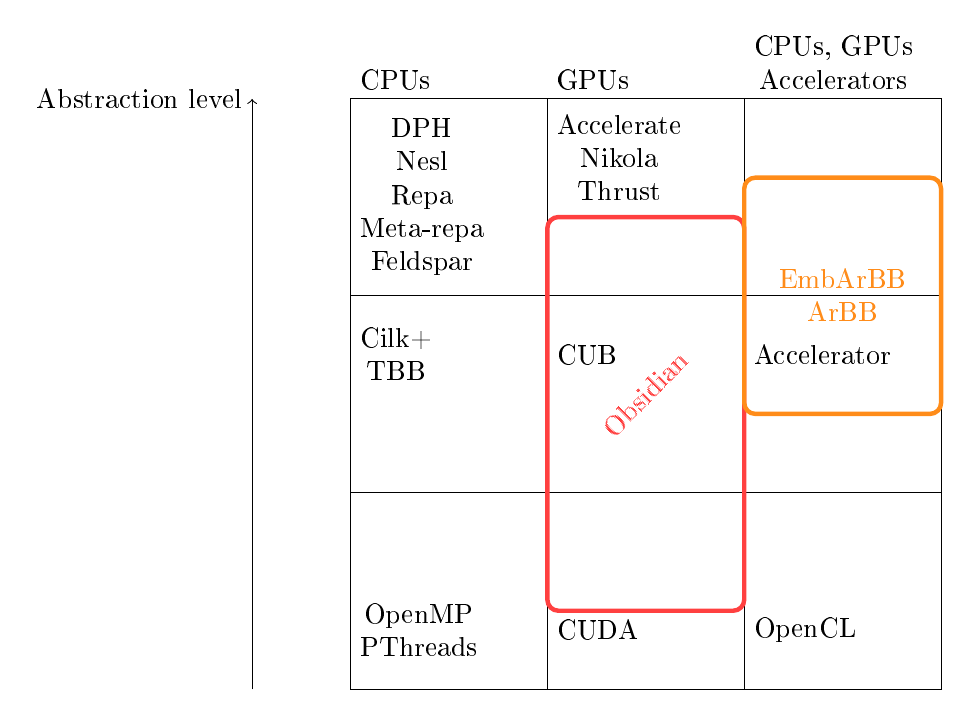
\begin{tikzpicture}[align=center, scale=2.5]
% \draw[help lines] (0,0) grid (3,3);


\draw[->] (-0.5,0) -- (-0.5,3) node[anchor=east] {Abstraction level};

\draw (0,3) node[anchor=south west] {CPUs};
\draw (1,3) node[anchor=south west] {GPUs};
%\draw (2,3) node[anchor=south west] {Accelerator};
\draw (2,3) node[anchor=south west] {CPUs, GPUs\\ Accelerators};

\node[anchor=west] (acc) at (1,2.7) {Accelerate\\Nikola\\Thrust};
\node[anchor=west] (acc) at (1,1.7) {CUB};
\node[anchor=west] (repa) at (0,2.5) {DPH\\Nesl\\Repa\\Meta-repa\\Feldspar};
\node[anchor=west] (mixed) at (0,1.7) {Cilk+\\ TBB};
\node[anchor=west] (accelerator) at (2,1.7) {Accelerator};

\node[anchor=west] (cuda) at (1,0.3) {CUDA};
\node[anchor=west] (opencl) at (2,0.3) {OpenCL};

\node[anchor=west] (OpenMP) at (0,0.3) {OpenMP\\PThreads};

\foreach \x in {0,...,2} { 
  \foreach \y in {0,...,2} { 
    \draw (\x,\y) rectangle (\x+1,\y+1);
  }
}

\draw[red!75,rounded corners,ultra thick] (1,0.4) rectangle (2,2.4);
\node[red!75,rotate=45,thick] (obs) at (1.5,1.5) {Obsidian};

\draw[orange!90,rounded corners,ultra thick] (2,1.4) rectangle (3,2.6);
\node[orange!90,thick] (arbb) at (2.5,2) {EmbArBB\\ArBB};


\end{tikzpicture}
\end{center}
\caption{Placing our work in the landscape of languages and libraries for parallel 
general purpose programming of CPUs, GPUs or both. }
\label{fig:researchmatrix} 
\end{figure}


% ---------------------------------------------------------------------------
% ArBB EmbArBB
% ---------------------------------------------------------------------------
The ArBB and EmbArBB systems also provide a set of parallel primitives that the programmer
composes to build his application. I place ArBB and EmbArBB in a box slightly lower than 
Accelerate,  since while ArBB/EmbArBB also have built in reduction primitives, just like 
Accelerate, 
they are not general primitives. Where Accelerate has a single higher order reduction 
operation, ArBB/EmbArBB has \\ {\tt reduce\_add, reduce\_mul} and so on. Benefits of 
having ArBB embedded in Haskell compared to C++ are discussed in section~\ref{sec:EmbArBB}.
%I will go into 
%what benefits there are to having ArBB embedded in Haskell compared to C++ in 

% ---------------------------------------------------------------------------
% Microsoft Accelerator
% ---------------------------------------------------------------------------
Microsoft Accelerator~\citet{ACCELERATOR} is a language embedded in C\#. Accelerator has
data-parallel arrays and a set of aggregate operations (operations on entire arrays). The 
operations on data-parallel arrays are JIT-compiled to GPU code. Accelerator can also 
compile to multithreaded CPU code and make use of SIMD units of modern 
CPUs~\citet{ACCELERATORCPU}; this makes the Accelerator system related to ArBB. 

% ---------------------------------------------------------------------------
% Python systems
% ---------------------------------------------------------------------------
There are many embedded languages implemented in Python that make use of GPUs 
to improve performance. One example is Copperhead~\citet{copperhead}. Copperhead 
supports flat and nested data-parallelism via primitives such as {\tt map} and 
{\tt reduce}.  

% ---------------------------------------------------------------------------
% Repa, Meta-Repa 
% --------------------------------------------------------------------------- 

Repa (Regular Shape-polymorphic Arrays)~\citet{REPA} is a Haskell library for 
data-parallel programming. 
Repa uses the same array representation as Obsidian, in Repa called a delayed
array, which is a function from index to element. However, in Repa arrays have shape; 
they can be of any dimensionality and there are shape-polymorphic functions on these. 
For example, {\tt map} can be applied to an array of any shape. 

Meta-Repa~\citet{METAREPA} is a reimplementation of the Repa library using deep embedded language 
techniques. Meta-Repa programs build ASTs that are then compiled (using template 
Haskell) to Haskell code that uses low-level parts of the Repa library for its parallelism.
The Meta-Repa approach to implementing the Repa library 
gives inlining of operations for free, where Repa programs need to be annotated 
with pragmas to ensure inlining. On the other hand, in Meta-Repa the programmer 
needs to explicitly state when something should not be inlined (using a {\tt force} primitive).
This is related to our work on EmbArBB that also uses an existing library (ArBB) 
for its parallelism. In reference~\citet{FPCDSL}, a case is made for this style 
of embedding preexisting DSLs. 


% ---------------------------------------------------------------------------
% DPH, NESL 
% ---------------------------------------------------------------------------
Data-Parallel Haskell~\citet{DPH} and Nesl~\citet{NESL} are languages for 
nested data-parallelism. Both run on CPUs, but there is also work towards 
a GPU version of Nesl~\citet{NestedGPU}. 

% ---------------------------------------------------------------------------
% Delite, Vertigo 
% ---------------------------------------------------------------------------

Delite~\citet{DELITE} is an infrastructure for implementation of domain 
specific embedded languages. There is an extensible internal representation (IR,AST); 
the programmer extends some base IR with domain specific constructs. The Delite system 
has been used to implement domain specific embedded languages for machine learning, rendering, 
physics and other domains. Delite, being a framework and the languages implemented using it 
very domains specific, was impossible to place in the matrix (Figure~\ref{fig:researchmatrix}). 

\subsection{Embedded domain specific languages} 

Feldspar is an embedded language for digital signal processing~\citet{FELDSPAR}. Apart 
from using the syntactic library~\citet{SyntacticICFP12}, it is quite similar to Obsidian. 
There is a deeply embedded core language (called Core) and vectors as a shallow embedding 
on top of that, just like in Obsidian.

When we first started working on Obsidian, we used Lava~\citet{LavaICFP} as inspiration. 
We wanted to mimic the Lava programming style but generate GPU code. At first this worked quite 
well and most Obsidian programs superficially looked quite like Lava programs. We have diverged 
from this aspiration since realising that GPUs are quite a different story and performance 
requires more control of GPU architecture specifics. 

\subsection{Compiling Embedded Languages}

In paper A~(section \ref{sec:paperA}), we describe our method for compiling monadic embedded 
languages. This work is closely related to a method described in ``The Constrained Monad Problem''
by Sculthorpe and Gill~\citet{sculthorpe2013constrained}. In that paper, they solve a more 
general problem than just compilation, but our method is nice because it is easy to understand 
and solves a single problem and does it well. In ``Generic monad constructs'', Persson et al 
also solve the problem of compiling monads using a continuation monad. 

``Compiling Embedded Languages'' by Elliott and Finne has been a constant source of information 
and something we have referred to in almost all our work. This is, in my opinion, the paper to turn 
to for anyone starting out with compiled embedded languages. 

%\subsection{Parallelism} 

%\noindent\emph{DPH}\citet{DPH} \newline
%\noindent\emph{D.A.Accelerate}\citet{ACCELERATEDAMP11} \newline
%\noindent\emph{Nikola}\citet{NIKOLA}\newline
%\noindent\emph{Repa}\citet{REPA}\newline
%\noindent\emph{Meta-Repa}\citet{METAREPA}\newline
%\noindent\emph{ArBB}\citet{ARBB2011}\newline
%\noindent\emph{OpenCL}\citet{OpenCL}\newline
%\noindent\emph{CUDA}\citet{CUDA}\newline
%\noindent\emph{Microsoft Accelerator}\citet{ACCELERATOR}\newline
%\noindent\emph{Copperhead}\citet{copperhead}\newline
%\noindent\emph{Delite}\citet{DELITE}\newline
%\noindent\emph{A monad for deterministic parallelism (R. Newton)} \citet{MonadPar} \newline
%\noindent\emph{Nesl}\citet{NESL} \newline

%\subsection{Embedded domain specific languages} 



\FloatBarrier
% ---------------------------------------------------------------------------
% ---------------------------------------------------------------------------
%
% Future work
%
% ---------------------------------------------------------------------------
% ---------------------------------------------------------------------------
\section{Future work} 
\label{sec:thesisFUTURE}

Obsidian is a language for GPU kernel implementation, not complete applications. 
It is not as well integrated into Haskell as for example Accelerate. There are 
ways to execute Obsidian kernels from within Haskell (we have seen an example of this in 
section~\ref{sec:GPUPROGRAMMING}); the recommended work flow, 
however, is to generate the CUDA as text and write the host code by hand. This 
can be seen as both a shortcoming and a feature. It is hard to integrate 
Accelerate programs in larger applications written in other languages; when 
using Obsidian a kernel is generated and can be used as part of for example a library.  

Obsidian is also quite a low-level language. The programmer needs to know GPU details 
and is allowed to write programs at a level almost as low as CUDA, if it is desired. 
Paper E (section~\ref{sec:paperE}) contains examples of programming at this low level. 
One potential use of Obsidian could be as the code generating backend of high-level 
and very domain specific embedded languages. This could be a niche for Obsidian.  

Obsidian constrains the programmer into writing programs that we can easily compile to 
CUDA. This is done by modelling the GPU programming in types attached to programs. A 
currently ongoing master's project is investigating what effects removing these 
types have. It is clear that if the programmer is not constrained to writing flat 
(or very limited nested) programs, transformations are needed on the AST before 
generating CUDA code. 

Obsidian's support for warp level computations is work in progress. Currently, warp level 
computations are not as well integrated into the hierarchy as the block, thread and grid 
levels are. The warp abstractions 
offered also require more work in the code generating backend than those 
that correspond directly to CUDA concepts. The problem is that CUDA does not have 
a warp abstraction. Warps needs to be better integrated with the rest of Obsidian 
and the code generation required for warps needs more testing before being 
trustworthy and useful. When operational, warp level abstractions will help 
the programmer make better use of the GPU. 

%\noindent\emph{Improve on Warp level capabilities} 

%\noindent\emph{Improve expressivity, code performance} 

% ---------------------------------------------------------------------------
% ---------------------------------------------------------------------------
%
% Discussion
%
% ---------------------------------------------------------------------------
% ---------------------------------------------------------------------------

\section{Discussion} 

%\vspace{5mm} 

% \emph{This section will revised.} 

%\vspace{5mm}

This thesis contains two approaches to embedding a language for data-parallel programming 
in Haskell. EmbArBB embeds a preexisting library for data-parallelism in Haskell 
and, at little effort from us, very good performance is gained. The performance of 
EmbArBB is entirely due to all the optimisation expertise and effort that was invested in 
the ArBB system. We get all that expertise for free. What EmbArBB provides is a 
way for Haskellers to benefit from the ArBB system. ArBB and EmbArBB are based on a 
set of parallel primitives for the programmer to use and compose. Obsidian takes 
a different approach. Built in primitives are very few and very low level, such as 
sequential and parallel for loops. On top of the low-level capabilities, a library 
of high-level primitives can be built. The key is that we want the programmer to 
be able to specify how to implement these higher level abstractions. 

Looking at the related work, we see that almost all high level GPU programming 
languages provide abstractions of parallel primitives, aggregate operations, 
maps, folds and reductions, giving justification to our investigation of GPU 
programming without these. We believe that the GPU architecture is still volatile 
enough that there is no ``the right'' way of implementing these primitives. As of 
today, the programmer still needs to explore the design space and find a solution 
that performs well on a particular GPU. 

Performance of Obsidian kernels is often good and the Obsidian code that they 
are generated from is often shorter than corresponding CUDA programs. Obsidian 
programs differ from CUDA programs by describing whole programs. A CUDA programmer 
needs to take a leap from the single threaded program 
parameterised on thread ID, to what actually will happen when this program is 
run by hundreds or thousands of threads at once. The extensive indexing arithmetic 
often present in CUDA programs can make this leap a hard one. Similar programs 
in Obsidian could use operations on whole arrays such as {\tt map} or explicitly 
bounded parallel loops. 

Push arrays were invented by Koen Claessen and first implemented in Obsidian 
to provide more control over where computation takes place (which thread computes 
which element). Push arrays has since been experimented on by others and show up 
in Nikola~\citet{NIKOLAPUSH} and Feldspar~\citet{FELDSPARPUSH}. Push arrays appear 
in StreamHS~\citet{FPCDSL} and in ~\citet{MOA} as part of a multi-dimensional array 
calculus in Standard ML. 


% ---------------------------------------------------------------------------
% ---------------------------------------------------------------------------
%
% Thesis overview
%
% ---------------------------------------------------------------------------
% ---------------------------------------------------------------------------
%% \section{Thesis overview} 

%% %This thesis contains an introduction and a selection of papers. The introduction 
%% %gives background and context to the papers. 

%% The papers contained in this thesis fall in three categories. 
%% \begin{itemize} 
%% \item General EDSL methodology in chapter~\ref{chap:EDSLImplementation}. 
%% \item GPU Programming using an EDSL in chapter~\ref{chap:GPUProgramming}. 
%% \item Retargetable parallel programming in chapter~\ref{chap:ArBB}. 
%% \end{itemize} 
%% %In the following sections, each paper is given a short description. Hopefully 
%% %there is enough information to wet the appetite. 

%% \subsection{EDSL implementation papers} 

%% \subsubsection{\paperA: \\ \paperATitle} 

%% Authors: Josef Svenningsson and Bo Joel Svensson 

%% \vspace{5mm}

%% \noindent This paper describes a simple and compositional method for 
%% reification of monads. This is useful for compilation of 
%% monadic embedded languages. We use a simple robot control language 
%% as the example. Robot programs can be expressed using Haskell do notation 
%% and are compiled down to a simple first order program representation. 
%% There is also a graphical simulator available that runs the compiled 
%% code. The robot language and simulator are available at github: \\ 
%% \url{github.com/svenssonjoel/Robot}.

%% \subsection{GPU programming papers} 

%% \subsubsection{\paperB: \\ \paperBTitle}

%% Authors: Bo Joel Svensson, Mary Sheeran and Koen Claessen \newline

%% \vspace{5mm}

%% This is the first real paper about Obsidian, our embedded language for GPU 
%% programming. In this paper, we identify similarities between 
%% connection patterns in hardware and parallel computations on GPUs. 
%% We introduce a structured and compositional way to write data-parallel 
%% programs on a GPU.

%% Basic parallel building blocks are implemented in a monadic style and 
%% composed using a sequential composition operator {\tt ->-}. 

%% \subsubsection{\paperC: \\ \paperCTitle}

%% Authors: Bo Joel Svensson, Koen Claessen and Mary Sheeran \newline

%% \vspace{5mm}

%% In this paper we describe a version of Obsidian implemented with a 
%% a different internal representation of GPU programs. We realised that 
%% most of our kernels have similar shape; they are parallel operations 
%% composed in sequence interspersed with barrier synchronisations. The 
%% internal representation used here captures this case exactly. Programming 
%% is now done is a style resembling arrows. 


%% \subsubsection{\paperD: \\ \paperDTitle}

%% Authors: Koen Claessen, Mary Sheeran and  Bo Joel Svensson \newline

%% \vspace{5mm}

%% This paper introduces {\em Push} arrays, invented by Koen Claessen. This 
%% array representation targets specific performance problems that we want 
%% to solve with Obsidian. Here we have also gone back to using monadic 
%% style for programming in Obsidian. 


%% \subsubsection{\paperE: \\ \paperETitle} 

%% Authors: Josef Svenningsson, Bo Joel Svensson and Mary Sheeran \newline

%% \vspace{5mm}

%% This paper contains a sorting case study performed in Obsidian. It 
%% is however the algorithms that are in focus here. We describe 
%% an interesting variation on Counting sort that removes duplicate 
%% elements and is a nice fit for GPUs because of its reduced need for 
%% synchronisation. 

%% In order to implement these sorting algorithms, we added atomic operations 
%% to Obsidian. 

%% \subsubsection{\paperF: \\ \paperFTitle}

%% Authors: Bo Joel Svensson and Mary Sheeran \newline
%% \noindent \emph{This work has not yet been published.}
%% \vspace{5mm} 

%% \noindent 

%% In this paper, the most recent additions and improvements to Obsidian are 
%% described. Obsidian Programs are now parameterised on Hierarchy level. This forces
%% the programmer into writing programs that we know how to compile to a GPU easily 
%% (by limiting how parallel operations can be nested). The central part of this paper 
%% describes how to implement and optimise reduction kernels using Obsidian. 


%% \subsection{Retargetable parallel programming} 

%% \subsubsection{\paperG: \\ \paperGTitle}

%% Authors: Bo Joel Svensson and Ryan R. Newton

%% \vspace{5mm}

%% \noindent This position paper describes the work I did while on a 3 month internship at 
%% Intel. The main part of this work was implementation of Haskell bindings 
%% for the now retired Intel ArBB system. 

%% The paper also describes work we did towards implementing a backend for the 
%% Accelerate system using ArBB. We reached a proof-of-concept implementation 
%% capable of running some simple Accelerate programs using the ArBB backend.
%% However, much work would remain to be able to run the full scope of Accelerate 
%% programs on ArBB.  

%% \subsubsection{\paperH: \\ \paperHTitle}

%% Authors: Bo Joel Svensson and Mary Sheeran 

%% \vspace{5mm}

%% \noindent Here we explore another way to provide the capabilities of ArBB to the 
%% Haskell programmer. Rather than trying to use ArBB as a backend to Accelerate 
%% we provide a more direct mapping of ArBB's functionality to Haskell idioms. 
%% We call this embedded language EmbArBB and it provides a more Haskell-programmer-friendly 
%% interface compared to the raw ArBB bindings (which are a collection of functions 
%% in the IO monad). 

% ---------------------------------------------------------------------------
% ---------------------------------------------------------------------------
%
% BIBLIOGRAPHY
%
% ---------------------------------------------------------------------------
% ---------------------------------------------------------------------------

\bibliographystylet{alpha}
\bibliographyt{thesis}
%\addcontentsline{toc}{section}{Bibliography}




\clearpage{}

% --------------------------------------------------------------------------- %
% --------------------------------------------------------------------------- %
%
%  PAPERS 
%
% --------------------------------------------------------------------------- %
% --------------------------------------------------------------------------- %


\chapter{EDSL Implementation Papers}
\label{chap:EDSLImplementation}
% ---------------------------------------------------------------------------
% 
% ---------------------------------------------------------------------------
\cleardoublepage 


\section[\paperATitle]{\paperA: \\ \paperATitle}
\label{sec:paperA}
%\addcontentsline{toc}{chapter}{Simple and Compositional Reification of Monadic Embedded Languages}

% \paperATitle

\begin{center} 
Josef Svenningsson, Bo Joel Svensson
\end{center}



%% bare_conf.tex
%% V1.3
%% 2007/01/11
%% by Michael Shell
%% See:
%% http://www.michaelshell.org/
%% for current contact information.
%%
%% This is a skeleton file demonstrating the use of IEEEtran.cls
%% (requires IEEEtran.cls version 1.7 or later) with an IEEE conference paper.
%%
%% Support sites:
%% http://www.michaelshell.org/tex/ieeetran/
%% http://www.ctan.org/tex-archive/macros/latex/contrib/IEEEtran/
%% and
%% http://www.ieee.org/

%\documentclass[conference]{IEEEtran}

%\usepackage{graphicx, color, code}
%\usepackage[cmex10]{amsmath}
%\usepackage{url}
% \usepackage{bookman}  %% bold teletype fonts, but don't know how to prevent it from changing the whole document

% Haven't figured out how to get this to work properly:
%\usepackage[\texttt{cmbtt}]{bold-extra}
% \usepackage{bold-extra} 

%\usepackage{courier}
%\usepackage{fancyvrb}

% correct bad hyphenation here
%\hyphenation{op-tical net-works semi-conduc-tor}


%====================================================================================================
%% FIRST, MISC USEFUL DEFINITIONS
%====================================================================================================

\definecolor{darkgreen}{rgb}{0, 0.5, 0}
\definecolor{darkblue}{rgb}{0,0,0.5}
\definecolor{mygrey}{rgb}{0.7,0.7,0.7}
\newcommand{\textblue}[1]{\textcolor{blue}{#1}}

\newcommand{\cde}[1]{{\footnotesize \tt #1}}

% \newcommand{\kw}[1]{{\bf{#1}}}
\newcommand{\kw}[1]{{\textbf{#1}}}

\newcommand{\comm}[1]{{\em \textcolor{darkgreen}{#1}}}  %% Code comments

\newcommand{\note}[1]{\begin{itemize}\item \textcolor{blue}{#1} \end{itemize}}

%% \newenvironment{mycode}
%% {% This is the begin code
%%   \begin{Verbatim}[commandchars=\\\{\}]}%
%%   %\footnotesize
%%   %\noindent
%%   %\begin{code}\noindent\vspace{-1mm}}
%% %  \begin{code}\noindent}
%% {% This is the end code
%%   \end{Verbatim}
%%   %\end{code} 
%% }

%% \newenvironment{inlinecode}
%% {
%%   \begin{center}
%%   \begin{minipage}{4in}
%%   \begin{mycode}
%% } 
%% {
%%   \end{mycode}
%%   \end{minipage}
%%   \end{center}
%%   \vspace{-1.5ex}
%% }

%% ============================================================
%% USE TO DISABLE COMMENTS:
 \def\noeditingmarks{}
%% ============================================================
\ifx\noeditingmarks\undefined
   \newcommand{\textred}[1]{\textcolor{red}{#1}}
   \newcommand{\pgwrapper}[2]{\textred{#1: #2}}
%   \newcommand{\pgwrapper}[2]{}
   \newcommand{\rnote}[1]{\begin{itemize}\item{\textcolor{blue}{#1}}\end{itemize}}
   \newcommand{\new}[1]{\textcolor{blue}{#1}}
   \newcommand{\const}[1]{\textred{#1}}

%% RRN: Dim the background for Ryan's eyes:
%%   What I need here is a way to do it based on user or host name...
% \pagecolor{mygrey}

\else
   \newcommand{\textred}[1]{#1}
   \newcommand{\pgwrapper}[2]{}
   \newcommand{\rnote}[1]{}
   \newcommand{\new}[1]{#1}
   \newcommand{\const}[1]{#1}
\fi

\newcommand{\js}[1]{\pgwrapper{BJS}{#1}}
\newcommand{\rn}[1]{\pgwrapper{RRN}{#1}}


%% Can we call our ``things'' 
%% ArBB/Haskell for the bindings part ? 
%% Accelerate/ArBB for the Accelerate backend ?
%% This would work with the convention we adopted for 
%%      ArBB/C++  
\newcommand{\systemname}[0]{{Harbb}}
%\newcommand{\systemname}[0]{\textred{HArBB}}

%% This could in theory be separate from the project name..
\newcommand{\accarbb}[0]{\systemname{}}

%% NOTE: THIS SHOULD BE THE SAME AS SYSTEMNAME:
\newcommand{\arbbvmH}[0]{ArBB/Haskell}


%====================================================================================================
% END DEFINITIONS
%====================================================================================================




%\begin{document}
% \title{Painless Portable Vector Parallelism\\ with Haskell and Intel ArBB}
%\title{Programming Future Parallel Architectures\\ with Haskell and Intel ArBB}
% \title{Embedded Domain-Specific Languages Pave the Way for New Parallel Architectures}

%\author{\IEEEauthorblockN{Bo Joel Svensson}
%\IEEEauthorblockA{Dept. of Computer Science and Engineering\\
%Chalmers University of Technology\\
%Gothenburg, Sweden\\
%Email: joels@chalmers.se}
%\and
%\IEEEauthorblockN{Ryan Newton}
%\IEEEauthorblockA{Intel Corporation\\
%Hudson, MA\\
%Email: rrnewton@gmail.com
%}}
% Email: ryan.r.newton@intel.com

%\maketitle

%\begin{abstract}
%
\subsection*{Abstract}
New parallel architectures, such 
\new{as Cell, Intel MIC, GPUs, and tiled architectures, enable} high
performance but are often hard to program.
What is needed is a bridge between high-level programming models 
where programmers are most productive and modern parallel architectures. 
We propose that that bridge is Embedded Domain Specific Languages (EDSLs). 

\new{One attractive target for EDSLs is}
Intel ArBB, a virtual machine for parallel, vectorized computations.
% that serves as a compilation target for EDSLs.
We propose to wed ArBB with the functional programming language
Haskell, {using an EDSL} that generates code for the ArBB VM.  This Haskell integration provides 
% a determinism guarantee 
added safety guarantees compared to other ArBB interfaces.
%
Further, our prototype, \systemname{}, is one of the first EDSL implementations with
optimized backends for multiple parallel architectures (CPU, \new{NVIDIA GPU}, and
others), allowing portability of source code over devices
and their accelerators.


%\end{abstract}
%\IEEEpeerreviewmaketitle




% ====================================================================================================
\subsection{Introduction}
% ====================================================================================================

Are radical new parallel architectures market-feasible if they require
significant changes for programmers?  The jury is out.  In recent
years we have seen difficult-to-program chips suffer 
% \citearbb{cell} 
(e.g. Cell)
and
GPU vendors strive to enable more traditional programming features
\citearbb{fermi} (e.g. C++).  There is an increasing
tension between ease of programming and efficiency.

The tension  shows  across diverse chip markets.  For example,
small embedded devices are most power efficient if their processors and operating systems
omit programming features such as virtual memory and threads \citearbb{tinyos}.  
At the other end of the power spectrum, GPU's
graphics performance may suffer due to inclusion of hardware to ease
GPGPU programming.  In short, there is an opportunity cost to
including extra hardware for programmability.

In this paper, we argue 
that a specific technique holds the greatest promise of solving the programmability dilemma.
%
Domain-specific languages, {\em embedded} within general purpose
languages (EDSLs) 
 enable familiar programming models 
{\em and} flexible
mapping onto new hardware.  The key to having this cake and eating it
too is {\em metaprogramming}.  Familiar programming features are
present, but are eliminated at an intermediate (metaprogram evaluation)
phase and therefore do not reach the parallel hardware itself.


% We present our ongoing work on a
In pursuit of this vision, we offer a
% 
 new EDSL implementation, called \accarbb{}, that combines
existing systems, Accelerate \citearbb{ACCELERATEDAMP11} and ArBB \citearbb{ArBB}, to produce a unified
high-level programming environment equally suited to multicore,
vectorized CPUs, as to GPUs and other accelerators (such as Intel MIC chips \citearbb{larrabee}).
%
\if{0}
ArBB is based on the RapidMind \citearbb{RapidMind} system which was an embedded 
DSL targeting multicore CPUs as well as GPUs. ArBB does not \new{yet} include a GPU 
backend like RapidMind, targeting multicore CPUs and their vector 
units. 
\fi{}
\systemname{} is a single EDSL implementation 
with independently optimized backends \new{by different teams; 
namely, the ArBB backend for CPU/MIC, and a CUDA backend for NVIDIA GPU.}
This makes
\systemname{} an appealing platform for fair CPU/GPU comparisons, 
as well as a compelling programming model for single-source portable performance across a range of
parallel architectures, \new{present and future}.
%%To our knowledge, \systemname{} is the first EDSL implementation with
%%independently optimized backends for CPUs and GPUs.  This makes
%%\systemname{} an appealing platform for fair CPU/GPU comparisons, 
%%as well as a compelling programming
%%model for single-source portable performance across a range of
%%parallel architectures.


% ====================================================================================================
\subsection{Embedded Domain-Specific Languages}
% ====================================================================================================


Domain-specific languages---from Makefiles and \LaTeX{} to
Matlab---are almost too ubiquitous to notice.  Most relevant to our
purposes, domain-specific languages (DSLs) that target a narrow domain and expose communication
patterns to the compiler 
 have achieved performance-portability across a wide range of parallel
architectures.  
StreamIt\citearbb{streamit} is a good example.
% (for example, StreamIt\citearbb{streamit})
% The high-water mark in this area is perhaps  StreamIt\citearbb{streamit}.
% 

% It has been noted \citearbb{not-sure} that 
% Yet the few DSLs that gain popularity lose simplicity\citearbb{not-sure}.  
% Yet popular DSLs rarely remain simple \citearbb{not-sure}.  
DSLs may start out simple and focused, but if they gain popularity
they quickly grow in complexity to rival full-blown languages.
Feature creep
can make DSL implementations complex and expensive to maintain.
Further, non-standard DSL syntax and features present a learning curve for users.  In the
last ten years an attractive solution to this dilemma has emerged: {\em
  embed} each DSL into a general-purpose host language that can provide
common functionality with familiar syntax and semantics.
% in place of the DSL.

When embedding, host language programs {generate} DSL programs;
% Embedding means that the host language is used to generate DSL programs; 
the {\em deeper} the embedding, the more integrated the
DSL into the syntax and type-system of the host language.
%
% Typically, %% pruning weasel words
A key host-language feature for embedding is that
language constructs can be overloaded to operate over {\em abstract
  syntax trees} (ASTs)\footnote{This ad-hoc polymorphism is accomplished,
for example, through operator-overloading in C++ or type classes in
Haskell.}.  For example, the following simple function operates on scalars:


\vspace{1mm}
\begin{Verbatim}[commandchars=\\\{\}]
  float f(float x) \{ return (2*x - 1); \}
\end{Verbatim}
\noindent
But simply by changing the types, \cde{f} might be lifted to operate on {\em
  expressions} (which, when evaluated, will yield \cde{floats}):

\vspace{1mm}
\begin{Verbatim}[commandchars=\\\{\}]
  \kw{exp<float>} f(\kw{exp<float>} x) \{
    return (2*x - 1);
  \}
\end{Verbatim}

A common arrangement is for the host language program to execute at
runtime but to generate ASTs that are executed by a just-in-time
(DSL) compiler.  This use of metaprogramming (program generation)
differs from the more common usage of preprocessors and 
% Lisp/Scheme macros \citearbb{scheme-macros}
macros, which typically add extra
phases of computation {\em before}  compile time---increasing
the number of compile-time rather than runtime phases.

% EDSLs typically add additional runtime phases.  That is, the host language program 
% executes at runtime but uses a JIT to process generated ASTs.
%% which are
%% usually used to perform computation {\em earlier} than the usual
%% compile time, embedded DSLs (EDSLs) typically defer computation 


One reason that EDSLs are good for productivity is that the programmer
gains the software engineering benefits of the host language
(object-orientation, higher-order-functions, modules, etc), while not
paying the cost at runtime for additional layers of abstraction or
indirection.  Indeed, the embedded languages for 
performance-oriented EDSLs are often simple, first-order
languages without pointers \citearbb{wavescript, ACCELERATEDAMP11}.

% , paul-lius-thingy

% regiment,
As a research area, EDSLs and two-stage DSLs have been actively pursued for at least a
decade \citearbb{VERTIGO, wavescript} but are gaining steam
recently 
%\citearbb{sejits, stanford-ppl} 
\citearbb{copperhead, stanford-ppl} 
and are beginning to appear in
commercial products \citearbb{ArBB}.
%
Further, EDSL techniques have spread beyond their origin in 
 the programming languages community.
% 
For example, both Stanford's Parallel Programming Laboratory (PPL) and
the Berkeley Parlab are creating EDSLs as their flagship parallel
programming solutions for domains such as machine learning and
rendering \citearbb{stanford-ppl}.
  Moreover, EDSLs need not be hosted by esoteric research languages---Intel's
 ArBB embeds an array language in C++ and Berkeley's
Copperhead \citearbb{copperhead} generates CUDA from simple Python code.

%\rnote{Is there a good motivating example program?  What are some of
%  the Metaocaml motivating examples?}

{For the remainder of this paper we will focus our discussion
  on the Intel ArBB VM, a virtual machine for just-in-time
  generation of vector codes, \new{which implements a restricted} domain-specific
  language of array computations.  In this paper we introduce
  {\em High-level ArBB}, 
  (\systemname{}), an EDSL that internally uses the ArBB
  VM.  \new{While Intel's ArBB package already includes an EDSL targeting the VM (for C++)},
\systemname{} \new{offers additional advantages, including}
  more succinct programs and additionally safety
  guarantees---namely, complete deterministic-by-construction parallel
  programs (across both host and VM languages).}


% ====================================================================================================
% \section{Accelerate and ArBB}
%\section{\accarbb{}:  ArBB and Accelerate}
\subsection{\accarbb{} $=$ ArBB $+$ Accelerate}
\label{sec:accelerate-arbb}
% ====================================================================================================

Our first \systemname{} prototype adapts an existing EDSL called {\em
  Accelerate} (Data.Array.Accelerate).  Accelerate targets high-level
data-parallel programming in Haskell.
Previous work on Accelerate has focused on developing a CUDA-backend
for GPU programming.  In this paper we describe our effort to retarget
Accelerate to ArBB.  

With respect to determinism guarantees, the existing Intel ArBB product
represents an integration of the safe (ArBB VM) with the unsafe (C++).
In the Haskell context, because purely functional computations are
guaranteed deterministic (even when executed in parallel), and because
ArBB computations invoked by Haskell functions are themselves free of
side-effects, \systemname{} achieves a
guarantee of determinism for complete programs that combine both
Haskell computation and ArBB VM computation.
% which offers portability.
% (The 'H' in \systemname{} therefore stands for Haskell as well as ``High-level''.)


%% {\em Accelerate} (Data.Array.Accelerate) is an existing EDSL for 
%% high-level data-parallel programming in Haskell~\citearbb{Accelerate}. 
The Accelerate programming model consists of collective 
operations that can be performed over arrays, together with a simple 
language of scalar expressions\new{---in the current release, the Haskell type system enforces that parallelism not be nested.}
\if{0}
The Haskell type 
system is used to enforce that no nested data-parallelism can be expressed 
\new{(in the current release, this may be relaxed in the future).}
\fi{}
Accelerate's collective operations include {\em Map} (akin to parallel
for loops) {\em ZipWith} (a generalization of elementwise vector addition) and 
{\em Fold} (sum generalized)---familiar operations for programmers versed in the functional paradigm.
All of these collective operations are easily parallelizable. 
% In the case of {\em Map} and {\em ZipWith} the potential for parallelism is abundant.  

%% dotProd :: Vector Float -> 
%%            Vector Float -> 
%%            Acc (Scalar Float) 
\begin{Verbatim}[commandchars=\\\{\}]
dotProd (xs :: Vector Float) 
        (ys :: Vector Float) = 
  \kw{let} xs\_ = use xs 
      ys\_ = use ys 
  \kw{in}  fold (+) 0 (zipWith (*) xs\_ ys\_) 
\end{Verbatim}

The Accelerate code listing above specifies a function that takes two 1-dimensional 
arrays as inputs (of type \cde{Vector Float}, e.g. a vector of floats). The result of the function is a single
scalar. 
% (\cde{Scalar Float})
The \cde{use} function is applied to an array to convert it 
for use in the collective operations provided by Accelerate;
\cde{use} 
% is actually a function with type \cde{Vector a -> Acc (Vector a)} and 
may result in
copying the array to, for example, the GPU in the case of Accelerate's 
CUDA backend.  

After applying \cde{use} to bring in input data, the programmer then
constructs a data-parallel program from collective operations.
Above, \cde{fold} is a function that takes three arguments, 
here those arguments are \cde{(+)},  $0$ and \cde{zipWith (*) xs\_ ys\_}. 
\cde{zipWith}, in turn, is a function taking three arguments, \cde{(*)}, 
\cde{xs\_} and \cde{ys\_}. The \cde{zipWith} operation here applies pairwise 
multiplication to the two arrays and the \cde{fold} sums up all the elements 
into a single scalar. 

%\rn{Following para slightly redundant but ok...}
%Accelerate makes GPU programming accessible to the functional programmer 
%by offering a familiar set of operations. This set of operations also have 
%the beneficial property that they have inherent parallelism and are 
%easily implementable on the GPU. 

Accelerate's CUDA backend implements collective operations using
a hand-tuned ``skeleton'' for each operation (and possibly for
different hardware versions). The kernel---for example, the function
to mapped over the dataset---is 
instantiated into the body of the skeleton code. The resulting 
program is compiled using the NVIDIA CUDA compiler and dynamically linked 
into the running Haskell program.

%\subsection{Intel Array Building Blocks (ArBB)}
\subsection{Intel Array Building Blocks (ArBB)}
\label{sec:arbb}

%ArBB is embedded in the C++ programming language but it also exposes a 
%very low level API that is purely C. 
%{\em ArBB} (Array Building Blocks) is also an embedded DSL. 
The operations exposed by ArBB are similar to those of Accelerate. 
In ArBB, parallel computations are expressed using a set of built-in 
primitives. All vectorization and threading is managed internally by 
ArBB. The programmer uses collective operations with a clear semantics 
such as \cde {add\_reduce} that computes the sum of the elements in a given 
array. ArBB also has language constructions for control flow, conditionals
and loops. These operations have their usual sequential semantics and are not 
parallelized by the system, rather, only specific collective operations are executed
in parallel. 

Today's existing ArBB product is embedded in C++ and provides special
types for scalars and arrays (e.g. \cde{dense<f32>} rather than \cde{vector<float>}).
Using ArBB/C++ to express the dot product computation can be done 
as follows:

%\vspace{2mm}
\begin{Verbatim}[commandchars=\\\{\}]
\kw{void} dot\_product(\kw{const} dense<f32>& a, 
                 \kw{const} dense<f32>& b,
                 f32& c) 
{ 
  c = add\_reduce(a * b);
}
\end{Verbatim} 


% The above program takes two arrays of type \cde{dense<f32>} as input. 
% \cde{dense<f32>} specifies a 1-dimensional array of 32-bit floating
% point values. The result is a single 32-bit float.  

Note that arithmetic operators such as (*) are overloaded 
for to operate on arrays as well as scalars (e.g. \cde{a * b} above).
Thus, the above C++ function multiplies two arrays before summing them with \cde {add\_reduce}:

The code listing below is indicative to the amount of glue code needed to invoke an 
ArBB computation\footnote{In OpenCL and CUDA the glue code situation is even worse}. It shows how the dot product code is launched using {\tt call} and 
how data is bound, {\tt bind}, for use in ArBB. 

\vspace{2mm}
\begin{Verbatim}[commandchars=\\\{\}]
\kw{int} main() 
\{ 
  double a[SIZE];
  double b[SIZE];

  for ( \kw{int} i = 0; i < SIZE; ++i) \{ 
    a[i] = ...; b[i] = ...;
  \}
  dense<f32> va, vb;
  f32 vc;
  bind(va, a, SIZE); 
  bind(vb, b, SIZE); 
  call(dot\_product)(va, vb, &vc); 
  ...
\}
\end{Verbatim}


%\rnote{SPECIFICALLY ADDRESS THE FUNCTIONALITY GAP?  E.G general
%  reduce.  Any other examples?}

The model provided by Accelerate is slightly richer than that of ArBB.
Even the two very simple \cde {dot\_product} examples above manage to illustrate 
this. In Accelerate there is a more general reduction primitive called \cde {fold} 
where in ArBB there are specific reductions, \cde {add\_reduce}, \cde {mul\_reduce} 
and so on. Not visible in these small examples is another difference, Accelerate 
operations are generalized to arbitrary dimensions while ArBB operations are 
limited to 1, 2, and 3 dimensions (and 0, i.e. scalar). These differences aside,
the ArBB and Accelerate programming models are very similar.


% ====================================================================================================
\subsection{Implementation of \systemname{}} 
% ====================================================================================================


%\rnote{Sadly the Haskell details don't buy us much here... what are
%  the {\em conceptual} problems solved in mapping the Accelerate
%  abstraction to the ArBB one?  The data models are similar, but
%  there are always mismatches -- dimensionality support, missing
%  reduction.}

%\rnote{What is the technique that you are using to address these sorts
%  of problems?  Is there anything to say about it?}

\begin{figure}
  \begin{center}
   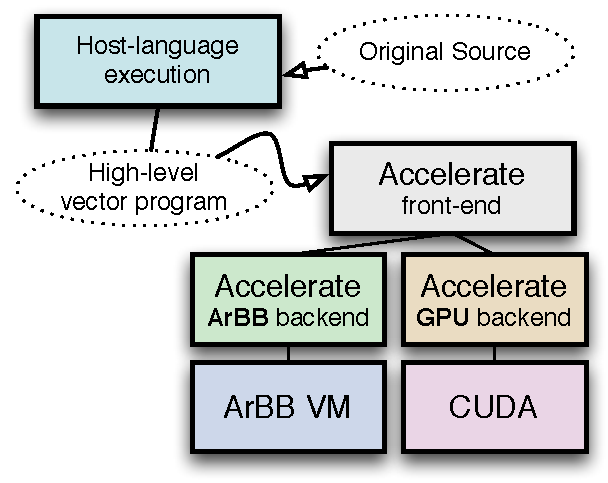
\includegraphics[width=2.0in]{./arbb/figure_architecture}    
  \end{center}
\vspace{-5mm}
  \caption{Architecture of the \systemname{} system.  \rn{(ROUGH.)}}
  \label{f:architecture}
\end{figure}


Using Accelerate and ArBB together, we propose a layered architecture
for \systemname{},
% Our goal is to make the benefits of ArBB available to the Haskell programmer. 
% \js{(Or is our goal to give an even better ``front-end'' to ArBB compared to C++)}
% We propose that this is best accomplished using a layered approach, as
pictured in Figure~\ref{f:architecture}. 
The host language execution (via Haskell in this case) executes the
programmer's source code, generating a vector program in the
restricted language of the Accelerate front-end.
Then either Accelerate backend---ArBB or CUDA---may be used.
The 
bottom layer of the ArBB backend consists of a direct mapping of the ArBB virtual machine
API (VMAPI) into Haskell including one-to-one bindings for each C 
function. 
To [partially] automate the creation of these bindings we used the C2HS system \citearbb{C2HS}. The 
\arbbvmH{} bindings are very low-level.
%and make little use of the high-level programming methods that
% Haskell programmers want. 
The idea 
is that the \arbbvmH{} bindings should be used to implement
backends for higher-level data-parallel EDSLs.

%% To illustrate our position we 
%% have started working on a backend to the successful DSL Accelerate 
%% (Data.Array.Accelerate) using our \arbbvmH{} bindings. 

To address the functionality mismatch between Accelerate and ArBB,
when possible we reencode the users Accelerate program using existing
ArBB mechanisms.  Our prototype does not support 100\% of Accelerate's
compute model (for example, only supporting  up to three-dimensional
arrays), but the remaining functionality can be mapped onto ArBB in
time using known methods---for example, our compiler could map higher
dimensional arrays onto a specific lower-dimensional data-layout.

%% The programming models supported by ArBB and Accelerate are very similar. 
%% Both obtain their parallelism by exposing collective operations 
%% such as {\em Map}, {\em Reduce}, {\em ZipWith} and {\em Scan} (all prefixes operations). However, 
%% the functionality match is not 100\%. For example, Accelerate supports {\em Map} operations 
%% over N-dimensional Arrays while ArBB supports them only up to 3-dimensions. 
%% Similar inconsistencies apply to the other operations as well. \textred{The current
%% ArBB backend simply disallows Accelerate programs using too high dimensionality
%% of the arrays.} \rn{Sure, we want to say that we're not done closing
%%   this gap (for
%%   accuracy) but more importantly we want to identify whether
%%   techniques exist to close the gap.  Presumably, yes?  We can
%%   ourselves collapse the dimensionality of arrays before giving them
%%   to ArBB?  Are there any operations that would defeat that technique?}
%

One example of a functionality discrepancy bridged by our
implementation is reductions.  As mentioned in \ref{sec:arbb},
Accelerate allows the programmer to reduce using an arbitrary
associative function, but ArBB has only built-in reductions with fixed
operations (add, multiply, xor, etc). We plan to provide general reductions in
the ArBB backend by a two-fold strategy:

\begin{enumerate}
\item Attempt to map an Accelerate reduction directly onto an ArBB
  primitive such as \cde{add\_reduce}.
\item Apply a general reduction technique based on $log(N)$ map
  operations over successively halving array sizes.  Essentially, cut
  the array in half, combine the halves, repeat. In ~\citearbb{reduction}
  this approach is explained in the context of CUDA. 
\end{enumerate}

%% \rn{Is the technique worthy of
%%   description?  Can we just cite the CUDA documentation or something
%%   since it's common?} 

In our current experiments, approach (2) is significantly slower.
Therefore, the ideal would be that ArBB exposed general reduction
directly in its programming model.  We expect this functionality to be
added in future releases.  In the meantime we plan to explore a
technique that would allow us to maximize the number of situations in
which (1) above applies.  Namely, a reduce operation can often be {\em
  factored} into a map followed by a reduce.  For example, a reduction
that multiplies each input number by a coefficient and sums the
results can be split into a map phase for the multiplication followed
by the built-in \cde {add\_reduce} operator.

%% Currently, our reduction implementations in ArBB 
%% are many times 
%% slower (\textasciitilde 20x) than their built-in counterparts. 
%% % To ameliorate this present performance problem we attempt to map
%% % programmers 
%% Our present workaround for this performance problem is to let 
%% \accarbb{} inspect the reduction function and switch to efficient 
%% built in  ArBB reduction where possible.  
%% \rn{Future work may be to decompose reductions into map+reduce so as
%%   to allow the reduce to become a builtin.}


Another choice faced by our implementation is the granularity at which the
ArBB JIT is invoked.  Specifically, should each collective operation result in its
own call to the ArBB JIT (in ArBB terminology, {\em
  immediate-mode}, akin to the pre-OpenGL 3.0 immediate mode), or
should multiple collective operations be placed together
inside an ArBB function and passed to the JIT?
We will call the latter approach {\em retained-mode}.

%% In immediate-mode the 
%% operations called from the ArBB API are executed
%% synchronously---before each API call returns. In retained-mode, ArBB
%% collects calls and, only when results are requested, the 
%% entire computation is optimized 
%% and executed. 

Retained-mode generally offers performance benefits; a bigger 
chunk is given to the JIT compiler, enabling cross-optimization
between collective operations. 
Our prototype Accelerate backend uses 
ArBB in  
a combination of immediate- and retained-mode. The main collective 
operations are compiled using the retained-mode. For example, in the case 
of a \cde{map f}  operation first the function to be mapped is created and 
compiled using retained-mode then a small {\em mapper} function is 
also created and compiled using retained-mode. 
%% The mapper function is 
%% of course very small and therefore does not give much to the JIT compiler 
%% to work on optimization-wise. 
Between the collective operations the backend
needs to perform data management and copying, which 
are performed in immediate-mode. It is our belief that 
\systemname{} would benefit from using retained-mode exclusively 
but we leave that as future work. 





% ====================================================================================================
\subsection{Preliminary Results}
% ====================================================================================================

%\rnote{One tiny benchmark if we can manage it.}

%\rnote{Ideally: Something like blackscholes running Arbb/C++,
%  \systemname{}, CPU+GPU, possibly compared to other blackscholes
%  implementations -- say Cilk on CPU and hand-coded CUDA (I can
%  provide the former I think).  Perhaps serial, non-vectorized CPU for
%  comparison.}

%\rnote{Point 1 -- High level thing is within X\% of low level thing.
%  The usual.  But we also want to say that \systemname{} is no worse
%  than ArBB/C++ -- the metalanguage doesn't matter, be it Haskell,
%  Python, or C++.}

%\rnote{Point 2 -- It's important to do a good job on the CPU side.
%  Even if you don't beat GPU there's a big difference between
%  vectorizing/not-vectorizing (and using multicore of coarse).  Can't
%  be ignored.}

%\rnote{Bonus points -- if we could show how bad ``naive'' ports are that
%  would be nice.  How well does your C CPU code run on GPU unmodified
%  (or minimally ported)?}



%\rnote{CPU/GPU systems that do a good job of both.  Perhaps quickly
%  dismiss those that make no effort on the CPU side.}

Black-Scholes option pricing is a finance-related benchmark that has been used in similar
DSLs targeting GPUs \citearbb{ACCELERATEDAMP11, NIKOLA}. Since we are re-using the 
Accelerate front-end, we can directly use the Black-Scholes benchmark that 
is shipped with that system.  Figure \ref{fig:blackscholes} shows the
complete code listing for an Accelerate Black-Scholes function which
can be executed on GPUs or any processor targeted by ArBB.

% blackscholes :: Vector (Float, Float, Float) 
%
%                -> Acc (Vector (Float, Float))
%\fbox{

%       r     = \textit{constant} riskfree
%       v     = \textit{constant} volatility

\begin{figure}
\begin{footnotesize}
\begin{Verbatim}[frame=single, commandchars=\\\{\}]
blackscholes (xs :: Vector (Float,Float,Float)) = 
  map kernel (\textit{use} xs)

kernel x =
  \kw{let} (price, strike, years) = \textit{unlift} x
      r     = 0.02 \textsf{\textit{-- riskfree constant}}
      v     = 0.30 \textsf{\textit{-- volatility constant}}
      sqrtT = sqrt years
      d1    = (log (price / strike) + 
                   (r + 0.5 * v * v) * years) / 
              (v * sqrtT)
      d2    = d1 - v * sqrtT
      cnd d = d >* 0 ? (1.0 - cndfn d, cndfn d)
      cndD1 = cnd d1
      cndD2 = cnd d2
      expRT = exp (-r * years)
  \kw{in} \textit{lift} ( price * cndD1 - 
            strike * expRT * cndD2
          , strike * expRT * (1.0 - cndD2) - 
            price * (1.0 - cndD1))

cndfn d =
  \kw{let} poly  = horner coeff
      coeff = [0, 0.31, -0.35, 1.78, -1.82, 1.33]
      rsqrt = 0.39894228040143267793994
      k     = 1.0 / (1.0 + 0.2316419 * abs d)
  \kw{in} rsqrt * exp (-0.5*d*d) * poly k

horner coeff x = 
  \kw{let} madd a b = b*x + a
  \kw{in}  foldr1 madd coeff
\end{Verbatim}
\end{footnotesize}
\caption{Complete code listing for a Black-Scholes function expressed
  in Haskell syntax using the Accelerate and \systemname{} libraries.
  Invocations of the functions \cde{use}, \cde{lift} and \cde{unlift}
%  and \cde{constant} 
represent additional boilerplate added for
  conversion in and out of Accelerate types.  Specifically, \cde{lift} and
  \cde{unlift} convert tuples and handle the fact that Accelerate
  arrays of tuples are really implemented as tuples of arrays.
  Otherwise, the program is identical to a plain Haskell
  implementation.}
\label{fig:blackscholes}
\end{figure}


%% \end{code}
%%  %605993438
%% % horner :: Num a => [a] -> a -> a
%% \begin{code}
%% \footnotesize



The kernel of this algorithm performs arithmetic on triples of
floating point numbers, creating pairs of floats as results. The problem 
is embarrassingly parallel, consisting of independent computations
for every element of an array (a map).

\begin{figure}
  \begin{center}
   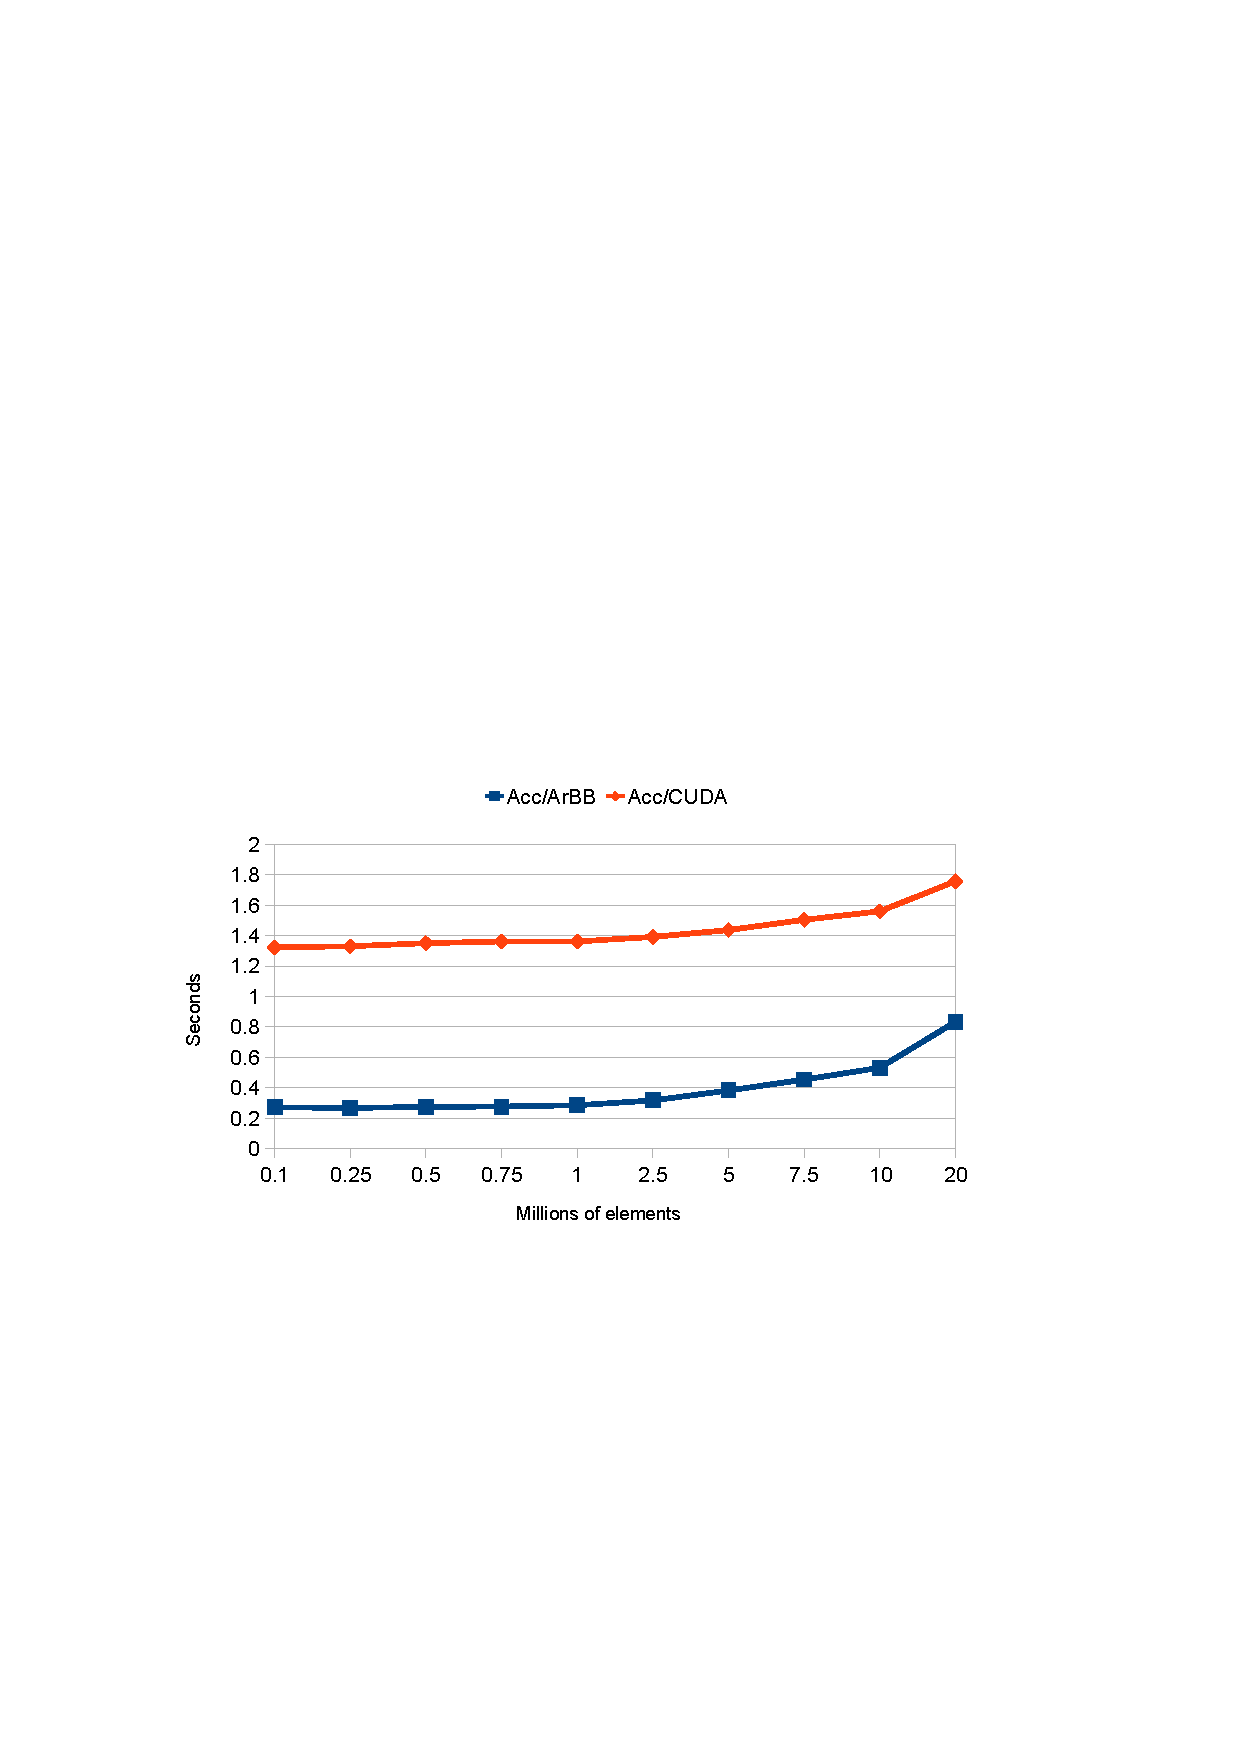
\includegraphics[width=3.5in]{./arbb/jit}    
  \end{center}
\vspace{-5mm}
  \caption{Running time experiments including JIT-time.} 
  \label{f:jit}
\end{figure}

\begin{figure}
  \begin{center}
   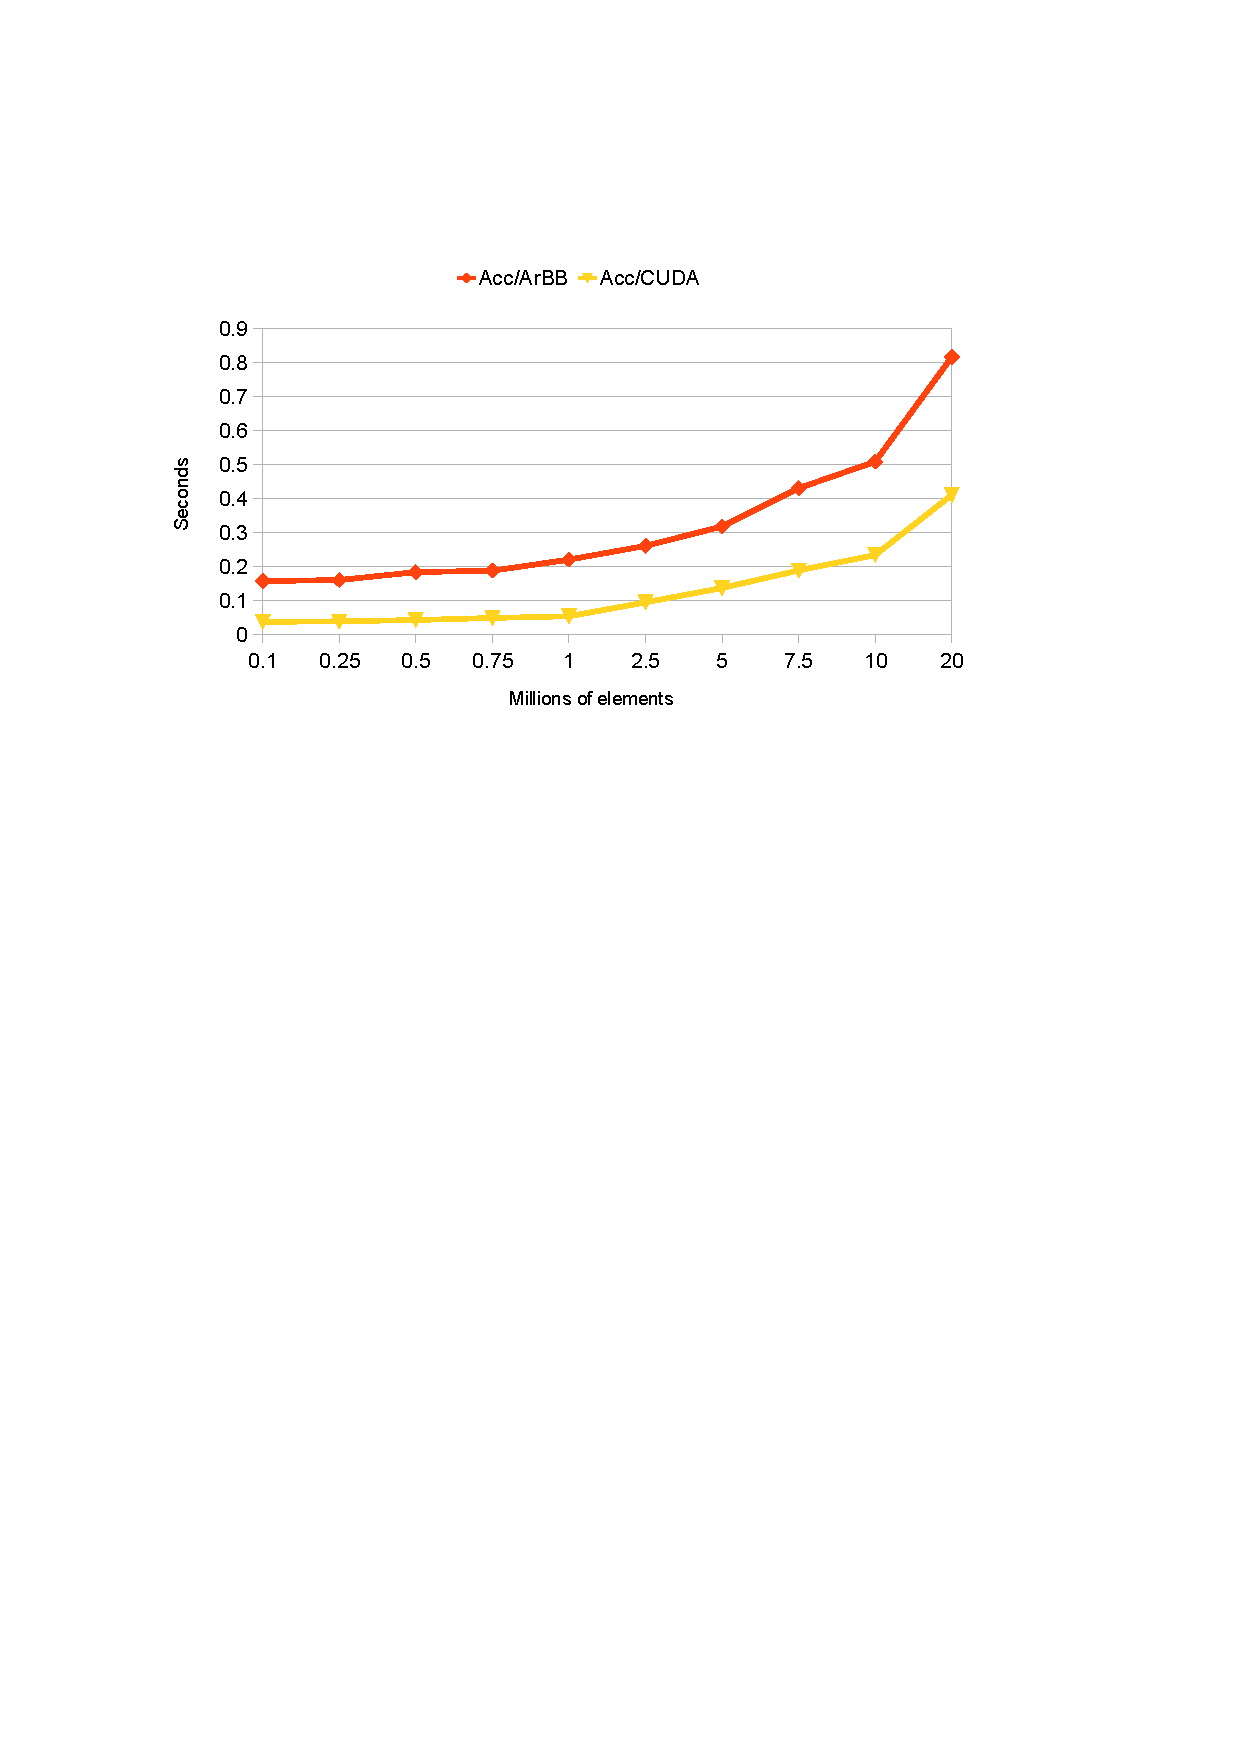
\includegraphics[width=3.5in]{./arbb/nojit}    
  \end{center}
\vspace{-5mm}
  \caption{Running time experiments JIT-time excluded.}
  \label{f:nojit}
\end{figure}


Figures~\ref{f:jit} and \ref{f:nojit} show preliminary results obtained on 
the Black-Scholes benchmark. The figures where obtained on a system with a 4-core 
Intel Core I7 975 machine with HyperThreading. The GPU used was a NVIDIA GTX480.

Figure~\ref{f:jit} shows running times obtained when JIT-time is included. 
% What this figure mainly tells us is that the JITing overhead 
JIT compilation time is much larger 
in the CUDA backend than the ArBB one.  Part of this difference 
can be attributed to the fact that 
the CUDA backend calls an external compiler (\cde{nvcc}), which takes its input in a file and runs in
a separate process.  ArBB, on the other hand, has a library interface to its  JIT-compiler. 
Figure~\ref{f:nojit} shows results obtained when pre-compiling the
CUDA functions eliminating JIT overhead.
In Accelerate, this happens automatically when the same kernel is
invoked repeatedly, because the Accelerate CUDA backed 
uses a caching scheme to avoid unnecessary JIT invocations.  (The
caching functionality has not yet been duplicated in the 
ArBB backend.)

These early results demonstrates the principle that even when a kernel
executes with higher throughput on a GPU, in a particular program it
is difficult to decide whether a computation is worth moving to a GPU,
incurring extra data-movement and possibly extra JIT compilation
\citearbb{wheres-the-data-paper}.  Specifically, we see that the
Accelerate Black-Scholes program from Figure~\ref{fig:blackscholes}
performs better on the CPU if it executes once (even on a large window
of data) whereas the GPU would yield better performance in a sustained
series of executions.
%
Because both CPU and GPU execution may be desirable---and the
selection may be dynamic---it is beneficial to have a single source code
that is portable across both.  
% Accelerate combined with \systemname{} makes this possible.


% ====================================================================================================
\subsection{Related Work}
% ====================================================================================================


OpenCL~\citearbb{opencl08} is a programming model very similar to CUDA but with the aspiration 
to offer both acceleration of computations on GPUs or to multicore CPUs. 
OpenCL JIT compiles the kernels for the particular hardware available and is
in that sense similar to ArBB.  
OpenCL programs are relatively low-level and require a large amount of
boilerplate to create and invoke.  In this sense they occupy a very
different niche than Accelerate.

Microsoft Accelerator~\citearbb{ACCELERATOR} is an embedded language with similar 
aspirations as ArBB, that is, to target a diverse range of architectures using the 
same source code. Accelerate can be used from the C\# language or the 
functional F\# language and targets GPUs or of CPUs and their
vector units.
% However, being part of the .Net framework implies limited accessibility 
%for platforms other than Microsoft Windows.  

\rn{What's the comparison with our stuff?}

%Most work on partitioning workloads between 
Many CPU and GPU comparisons, and some CPU/GPU workload partitioners \citearbb{merge}, rely on
redundant hand-written versions of all kernels
% \citearbb{cpu-gpu-partitioning} 
(though some systems like Qilin \citearbb{qilin} allow a single source code).
It is difficult in this kind of scenario
to make fair comparisons, controlling for the
amount of effort put into the respective implementations.
For example, comparing unoptimized serial CPU implementations vs. GPU
ones is not informative \citearbb{debunking-dubey}.
In \systemname{} controlling for effort
need happen only once---both CUDA and ArBB are
independently optimized by their respective teams of engineers---not for each benchmark.


% ====================================================================================================
% \section{Future work and Conclusions}
%\section{Future Work}
% ====================================================================================================

%\rn{need to be careful about being too repetitive...}
%The \accarbb{} backend is currently work-in-progress. The Accelerate
%functionality is not yet completely covered by the ArBB backend. Currently 
%the ArBB back-ed is operational for Accelerate programs using {\em Map}, 
%{\em ZipWith} and some simple instances of the Accelerate {\em Fold} operation.
%All of these also have the limitation that they only work for up to and 
%including 3-dimensional arrays using the ArBB backend while the Accelerate
%model allows the N-dimensional case. Allowing the N-dimensional case 
%in the ArBB backend for the supported operations range from a simple exercise 
%to more intricate problems needing some thought. For example, in the case 
%{\em Map} operations the needed transformation is simple (Accelerate Maps 
%over N-dimensional arrays is a per-element operation). One could flatten 
%the N-dimensional array to a 1-dimensional array (remembering its old shape) 
%perform the map and then transform the array back into N-dimensions. In 
%the case of {\em Fold} (reductions) the situation becomes more tricky. 
%transforming the arrays to arrays of lesser dimensionality then requires 
%a so-called segmented {\em Fold} operation. 

%The current \accarbb{} backend uses a hybrid of immediate-mode 
%and retained-mode programming styles. Moving more towards 
%retained-mode only may have performance benefits since it would give the 
%ArBB compiler larger programs to optimize. Exploring this aspect is left 
%as future work. 

% ====================================================================================================
\subsection{Discussion and Conclusions}
% ====================================================================================================

We have demonstrated that an EDSL such as Accelerate is sufficiently
platform-independent to break free of its original hardware target
(CUDA/GPU) and create efficient programs on other architectures.  This
gives us hope that \systemname{}/Accelerate programs will be
forward-portable to future parallel architectures and instruction
sets.

The EDSL approach changes the playing field for the designer
of compiler backends.  Rather than contending with full blown
languages and their complexities (e.g. pointers, aliasing,
inheritance, virtual functions, etc), compiler backends can focus on
simple value-oriented compute languages.

%% Achieving the ultimate goal of performance portability requires
%% progress on two research problems.  The first is EDSLs themselves and
%% their integration into host languages.  The second problem 

But the EDSL method solves only part of the performance-portability problem.
Simple as EDSL target languages may be, there remains a
substantial challenge in mapping them efficiently to the diversity
of parallel architectures available now and in the near future.
%especially without requiring a large amount of additional per-platform
%user annotations.
\textred{For example, the idiosyncrasies of memory bank access on
  NVIDIA GPUs must be taken into account to generate efficient
  implementations of the high-level collective operations that we have
  discussed.}

This is a compiler backend research challenge.
The {\em skeletons} method mentioned in
Section~\ref{sec:accelerate-arbb} is one approach to this problem, as
are the optimizations studied in the Copperhead \citearbb{copperhead} and
Obsidian \citearbb{JSLIC} projects.
%
On the other hand, systems that rely on advanced optimizations
typically suffer to some extent from performance-predictability
problems.  Thus achieving portable, predictable performance on a wide range
of architectures---even for the simplest target languages---will
be the subject of much future work.

%{
%\small
\bibliographystylearbb{alpha}
\bibliographyarbb{thesis}
%}


%\end{document}






\chapter{GPU Programming Papers}
\label{chap:GPUProgramming}

% ---------------------------------------------------------------------------
% 
% ---------------------------------------------------------------------------
\cleardoublepage 

\section[\paperBTitle]{\paperB: \\ \paperBTitle}
\label{sec:paperB}
%\addcontentsline{toc}{chapter}{Obsidian: A Domain Specific Embedded Language for
%Parallel Programming of Graphics Processors}

%\paperBTitle

\begin{center} 
Bo Joel Svensson, Mary Sheeran, Koen Claessen
\end{center}


%% bare_conf.tex
%% V1.3
%% 2007/01/11
%% by Michael Shell
%% See:
%% http://www.michaelshell.org/
%% for current contact information.
%%
%% This is a skeleton file demonstrating the use of IEEEtran.cls
%% (requires IEEEtran.cls version 1.7 or later) with an IEEE conference paper.
%%
%% Support sites:
%% http://www.michaelshell.org/tex/ieeetran/
%% http://www.ctan.org/tex-archive/macros/latex/contrib/IEEEtran/
%% and
%% http://www.ieee.org/

%\documentclass[conference]{IEEEtran}

%\usepackage{graphicx, color, code}
%\usepackage[cmex10]{amsmath}
%\usepackage{url}
% \usepackage{bookman}  %% bold teletype fonts, but don't know how to prevent it from changing the whole document

% Haven't figured out how to get this to work properly:
%\usepackage[\texttt{cmbtt}]{bold-extra}
% \usepackage{bold-extra} 

%\usepackage{courier}
%\usepackage{fancyvrb}

% correct bad hyphenation here
%\hyphenation{op-tical net-works semi-conduc-tor}


%====================================================================================================
%% FIRST, MISC USEFUL DEFINITIONS
%====================================================================================================

\definecolor{darkgreen}{rgb}{0, 0.5, 0}
\definecolor{darkblue}{rgb}{0,0,0.5}
\definecolor{mygrey}{rgb}{0.7,0.7,0.7}
\newcommand{\textblue}[1]{\textcolor{blue}{#1}}

\newcommand{\cde}[1]{{\footnotesize \tt #1}}

% \newcommand{\kw}[1]{{\bf{#1}}}
\newcommand{\kw}[1]{{\textbf{#1}}}

\newcommand{\comm}[1]{{\em \textcolor{darkgreen}{#1}}}  %% Code comments

\newcommand{\note}[1]{\begin{itemize}\item \textcolor{blue}{#1} \end{itemize}}

%% \newenvironment{mycode}
%% {% This is the begin code
%%   \begin{Verbatim}[commandchars=\\\{\}]}%
%%   %\footnotesize
%%   %\noindent
%%   %\begin{code}\noindent\vspace{-1mm}}
%% %  \begin{code}\noindent}
%% {% This is the end code
%%   \end{Verbatim}
%%   %\end{code} 
%% }

%% \newenvironment{inlinecode}
%% {
%%   \begin{center}
%%   \begin{minipage}{4in}
%%   \begin{mycode}
%% } 
%% {
%%   \end{mycode}
%%   \end{minipage}
%%   \end{center}
%%   \vspace{-1.5ex}
%% }

%% ============================================================
%% USE TO DISABLE COMMENTS:
 \def\noeditingmarks{}
%% ============================================================
\ifx\noeditingmarks\undefined
   \newcommand{\textred}[1]{\textcolor{red}{#1}}
   \newcommand{\pgwrapper}[2]{\textred{#1: #2}}
%   \newcommand{\pgwrapper}[2]{}
   \newcommand{\rnote}[1]{\begin{itemize}\item{\textcolor{blue}{#1}}\end{itemize}}
   \newcommand{\new}[1]{\textcolor{blue}{#1}}
   \newcommand{\const}[1]{\textred{#1}}

%% RRN: Dim the background for Ryan's eyes:
%%   What I need here is a way to do it based on user or host name...
% \pagecolor{mygrey}

\else
   \newcommand{\textred}[1]{#1}
   \newcommand{\pgwrapper}[2]{}
   \newcommand{\rnote}[1]{}
   \newcommand{\new}[1]{#1}
   \newcommand{\const}[1]{#1}
\fi

\newcommand{\js}[1]{\pgwrapper{BJS}{#1}}
\newcommand{\rn}[1]{\pgwrapper{RRN}{#1}}


%% Can we call our ``things'' 
%% ArBB/Haskell for the bindings part ? 
%% Accelerate/ArBB for the Accelerate backend ?
%% This would work with the convention we adopted for 
%%      ArBB/C++  
\newcommand{\systemname}[0]{{Harbb}}
%\newcommand{\systemname}[0]{\textred{HArBB}}

%% This could in theory be separate from the project name..
\newcommand{\accarbb}[0]{\systemname{}}

%% NOTE: THIS SHOULD BE THE SAME AS SYSTEMNAME:
\newcommand{\arbbvmH}[0]{ArBB/Haskell}


%====================================================================================================
% END DEFINITIONS
%====================================================================================================




%\begin{document}
% \title{Painless Portable Vector Parallelism\\ with Haskell and Intel ArBB}
%\title{Programming Future Parallel Architectures\\ with Haskell and Intel ArBB}
% \title{Embedded Domain-Specific Languages Pave the Way for New Parallel Architectures}

%\author{\IEEEauthorblockN{Bo Joel Svensson}
%\IEEEauthorblockA{Dept. of Computer Science and Engineering\\
%Chalmers University of Technology\\
%Gothenburg, Sweden\\
%Email: joels@chalmers.se}
%\and
%\IEEEauthorblockN{Ryan Newton}
%\IEEEauthorblockA{Intel Corporation\\
%Hudson, MA\\
%Email: rrnewton@gmail.com
%}}
% Email: ryan.r.newton@intel.com

%\maketitle

%\begin{abstract}
%
\subsection*{Abstract}
New parallel architectures, such 
\new{as Cell, Intel MIC, GPUs, and tiled architectures, enable} high
performance but are often hard to program.
What is needed is a bridge between high-level programming models 
where programmers are most productive and modern parallel architectures. 
We propose that that bridge is Embedded Domain Specific Languages (EDSLs). 

\new{One attractive target for EDSLs is}
Intel ArBB, a virtual machine for parallel, vectorized computations.
% that serves as a compilation target for EDSLs.
We propose to wed ArBB with the functional programming language
Haskell, {using an EDSL} that generates code for the ArBB VM.  This Haskell integration provides 
% a determinism guarantee 
added safety guarantees compared to other ArBB interfaces.
%
Further, our prototype, \systemname{}, is one of the first EDSL implementations with
optimized backends for multiple parallel architectures (CPU, \new{NVIDIA GPU}, and
others), allowing portability of source code over devices
and their accelerators.


%\end{abstract}
%\IEEEpeerreviewmaketitle




% ====================================================================================================
\subsection{Introduction}
% ====================================================================================================

Are radical new parallel architectures market-feasible if they require
significant changes for programmers?  The jury is out.  In recent
years we have seen difficult-to-program chips suffer 
% \citearbb{cell} 
(e.g. Cell)
and
GPU vendors strive to enable more traditional programming features
\citearbb{fermi} (e.g. C++).  There is an increasing
tension between ease of programming and efficiency.

The tension  shows  across diverse chip markets.  For example,
small embedded devices are most power efficient if their processors and operating systems
omit programming features such as virtual memory and threads \citearbb{tinyos}.  
At the other end of the power spectrum, GPU's
graphics performance may suffer due to inclusion of hardware to ease
GPGPU programming.  In short, there is an opportunity cost to
including extra hardware for programmability.

In this paper, we argue 
that a specific technique holds the greatest promise of solving the programmability dilemma.
%
Domain-specific languages, {\em embedded} within general purpose
languages (EDSLs) 
 enable familiar programming models 
{\em and} flexible
mapping onto new hardware.  The key to having this cake and eating it
too is {\em metaprogramming}.  Familiar programming features are
present, but are eliminated at an intermediate (metaprogram evaluation)
phase and therefore do not reach the parallel hardware itself.


% We present our ongoing work on a
In pursuit of this vision, we offer a
% 
 new EDSL implementation, called \accarbb{}, that combines
existing systems, Accelerate \citearbb{ACCELERATEDAMP11} and ArBB \citearbb{ArBB}, to produce a unified
high-level programming environment equally suited to multicore,
vectorized CPUs, as to GPUs and other accelerators (such as Intel MIC chips \citearbb{larrabee}).
%
\if{0}
ArBB is based on the RapidMind \citearbb{RapidMind} system which was an embedded 
DSL targeting multicore CPUs as well as GPUs. ArBB does not \new{yet} include a GPU 
backend like RapidMind, targeting multicore CPUs and their vector 
units. 
\fi{}
\systemname{} is a single EDSL implementation 
with independently optimized backends \new{by different teams; 
namely, the ArBB backend for CPU/MIC, and a CUDA backend for NVIDIA GPU.}
This makes
\systemname{} an appealing platform for fair CPU/GPU comparisons, 
as well as a compelling programming model for single-source portable performance across a range of
parallel architectures, \new{present and future}.
%%To our knowledge, \systemname{} is the first EDSL implementation with
%%independently optimized backends for CPUs and GPUs.  This makes
%%\systemname{} an appealing platform for fair CPU/GPU comparisons, 
%%as well as a compelling programming
%%model for single-source portable performance across a range of
%%parallel architectures.


% ====================================================================================================
\subsection{Embedded Domain-Specific Languages}
% ====================================================================================================


Domain-specific languages---from Makefiles and \LaTeX{} to
Matlab---are almost too ubiquitous to notice.  Most relevant to our
purposes, domain-specific languages (DSLs) that target a narrow domain and expose communication
patterns to the compiler 
 have achieved performance-portability across a wide range of parallel
architectures.  
StreamIt\citearbb{streamit} is a good example.
% (for example, StreamIt\citearbb{streamit})
% The high-water mark in this area is perhaps  StreamIt\citearbb{streamit}.
% 

% It has been noted \citearbb{not-sure} that 
% Yet the few DSLs that gain popularity lose simplicity\citearbb{not-sure}.  
% Yet popular DSLs rarely remain simple \citearbb{not-sure}.  
DSLs may start out simple and focused, but if they gain popularity
they quickly grow in complexity to rival full-blown languages.
Feature creep
can make DSL implementations complex and expensive to maintain.
Further, non-standard DSL syntax and features present a learning curve for users.  In the
last ten years an attractive solution to this dilemma has emerged: {\em
  embed} each DSL into a general-purpose host language that can provide
common functionality with familiar syntax and semantics.
% in place of the DSL.

When embedding, host language programs {generate} DSL programs;
% Embedding means that the host language is used to generate DSL programs; 
the {\em deeper} the embedding, the more integrated the
DSL into the syntax and type-system of the host language.
%
% Typically, %% pruning weasel words
A key host-language feature for embedding is that
language constructs can be overloaded to operate over {\em abstract
  syntax trees} (ASTs)\footnote{This ad-hoc polymorphism is accomplished,
for example, through operator-overloading in C++ or type classes in
Haskell.}.  For example, the following simple function operates on scalars:


\vspace{1mm}
\begin{Verbatim}[commandchars=\\\{\}]
  float f(float x) \{ return (2*x - 1); \}
\end{Verbatim}
\noindent
But simply by changing the types, \cde{f} might be lifted to operate on {\em
  expressions} (which, when evaluated, will yield \cde{floats}):

\vspace{1mm}
\begin{Verbatim}[commandchars=\\\{\}]
  \kw{exp<float>} f(\kw{exp<float>} x) \{
    return (2*x - 1);
  \}
\end{Verbatim}

A common arrangement is for the host language program to execute at
runtime but to generate ASTs that are executed by a just-in-time
(DSL) compiler.  This use of metaprogramming (program generation)
differs from the more common usage of preprocessors and 
% Lisp/Scheme macros \citearbb{scheme-macros}
macros, which typically add extra
phases of computation {\em before}  compile time---increasing
the number of compile-time rather than runtime phases.

% EDSLs typically add additional runtime phases.  That is, the host language program 
% executes at runtime but uses a JIT to process generated ASTs.
%% which are
%% usually used to perform computation {\em earlier} than the usual
%% compile time, embedded DSLs (EDSLs) typically defer computation 


One reason that EDSLs are good for productivity is that the programmer
gains the software engineering benefits of the host language
(object-orientation, higher-order-functions, modules, etc), while not
paying the cost at runtime for additional layers of abstraction or
indirection.  Indeed, the embedded languages for 
performance-oriented EDSLs are often simple, first-order
languages without pointers \citearbb{wavescript, ACCELERATEDAMP11}.

% , paul-lius-thingy

% regiment,
As a research area, EDSLs and two-stage DSLs have been actively pursued for at least a
decade \citearbb{VERTIGO, wavescript} but are gaining steam
recently 
%\citearbb{sejits, stanford-ppl} 
\citearbb{copperhead, stanford-ppl} 
and are beginning to appear in
commercial products \citearbb{ArBB}.
%
Further, EDSL techniques have spread beyond their origin in 
 the programming languages community.
% 
For example, both Stanford's Parallel Programming Laboratory (PPL) and
the Berkeley Parlab are creating EDSLs as their flagship parallel
programming solutions for domains such as machine learning and
rendering \citearbb{stanford-ppl}.
  Moreover, EDSLs need not be hosted by esoteric research languages---Intel's
 ArBB embeds an array language in C++ and Berkeley's
Copperhead \citearbb{copperhead} generates CUDA from simple Python code.

%\rnote{Is there a good motivating example program?  What are some of
%  the Metaocaml motivating examples?}

{For the remainder of this paper we will focus our discussion
  on the Intel ArBB VM, a virtual machine for just-in-time
  generation of vector codes, \new{which implements a restricted} domain-specific
  language of array computations.  In this paper we introduce
  {\em High-level ArBB}, 
  (\systemname{}), an EDSL that internally uses the ArBB
  VM.  \new{While Intel's ArBB package already includes an EDSL targeting the VM (for C++)},
\systemname{} \new{offers additional advantages, including}
  more succinct programs and additionally safety
  guarantees---namely, complete deterministic-by-construction parallel
  programs (across both host and VM languages).}


% ====================================================================================================
% \section{Accelerate and ArBB}
%\section{\accarbb{}:  ArBB and Accelerate}
\subsection{\accarbb{} $=$ ArBB $+$ Accelerate}
\label{sec:accelerate-arbb}
% ====================================================================================================

Our first \systemname{} prototype adapts an existing EDSL called {\em
  Accelerate} (Data.Array.Accelerate).  Accelerate targets high-level
data-parallel programming in Haskell.
Previous work on Accelerate has focused on developing a CUDA-backend
for GPU programming.  In this paper we describe our effort to retarget
Accelerate to ArBB.  

With respect to determinism guarantees, the existing Intel ArBB product
represents an integration of the safe (ArBB VM) with the unsafe (C++).
In the Haskell context, because purely functional computations are
guaranteed deterministic (even when executed in parallel), and because
ArBB computations invoked by Haskell functions are themselves free of
side-effects, \systemname{} achieves a
guarantee of determinism for complete programs that combine both
Haskell computation and ArBB VM computation.
% which offers portability.
% (The 'H' in \systemname{} therefore stands for Haskell as well as ``High-level''.)


%% {\em Accelerate} (Data.Array.Accelerate) is an existing EDSL for 
%% high-level data-parallel programming in Haskell~\citearbb{Accelerate}. 
The Accelerate programming model consists of collective 
operations that can be performed over arrays, together with a simple 
language of scalar expressions\new{---in the current release, the Haskell type system enforces that parallelism not be nested.}
\if{0}
The Haskell type 
system is used to enforce that no nested data-parallelism can be expressed 
\new{(in the current release, this may be relaxed in the future).}
\fi{}
Accelerate's collective operations include {\em Map} (akin to parallel
for loops) {\em ZipWith} (a generalization of elementwise vector addition) and 
{\em Fold} (sum generalized)---familiar operations for programmers versed in the functional paradigm.
All of these collective operations are easily parallelizable. 
% In the case of {\em Map} and {\em ZipWith} the potential for parallelism is abundant.  

%% dotProd :: Vector Float -> 
%%            Vector Float -> 
%%            Acc (Scalar Float) 
\begin{Verbatim}[commandchars=\\\{\}]
dotProd (xs :: Vector Float) 
        (ys :: Vector Float) = 
  \kw{let} xs\_ = use xs 
      ys\_ = use ys 
  \kw{in}  fold (+) 0 (zipWith (*) xs\_ ys\_) 
\end{Verbatim}

The Accelerate code listing above specifies a function that takes two 1-dimensional 
arrays as inputs (of type \cde{Vector Float}, e.g. a vector of floats). The result of the function is a single
scalar. 
% (\cde{Scalar Float})
The \cde{use} function is applied to an array to convert it 
for use in the collective operations provided by Accelerate;
\cde{use} 
% is actually a function with type \cde{Vector a -> Acc (Vector a)} and 
may result in
copying the array to, for example, the GPU in the case of Accelerate's 
CUDA backend.  

After applying \cde{use} to bring in input data, the programmer then
constructs a data-parallel program from collective operations.
Above, \cde{fold} is a function that takes three arguments, 
here those arguments are \cde{(+)},  $0$ and \cde{zipWith (*) xs\_ ys\_}. 
\cde{zipWith}, in turn, is a function taking three arguments, \cde{(*)}, 
\cde{xs\_} and \cde{ys\_}. The \cde{zipWith} operation here applies pairwise 
multiplication to the two arrays and the \cde{fold} sums up all the elements 
into a single scalar. 

%\rn{Following para slightly redundant but ok...}
%Accelerate makes GPU programming accessible to the functional programmer 
%by offering a familiar set of operations. This set of operations also have 
%the beneficial property that they have inherent parallelism and are 
%easily implementable on the GPU. 

Accelerate's CUDA backend implements collective operations using
a hand-tuned ``skeleton'' for each operation (and possibly for
different hardware versions). The kernel---for example, the function
to mapped over the dataset---is 
instantiated into the body of the skeleton code. The resulting 
program is compiled using the NVIDIA CUDA compiler and dynamically linked 
into the running Haskell program.

%\subsection{Intel Array Building Blocks (ArBB)}
\subsection{Intel Array Building Blocks (ArBB)}
\label{sec:arbb}

%ArBB is embedded in the C++ programming language but it also exposes a 
%very low level API that is purely C. 
%{\em ArBB} (Array Building Blocks) is also an embedded DSL. 
The operations exposed by ArBB are similar to those of Accelerate. 
In ArBB, parallel computations are expressed using a set of built-in 
primitives. All vectorization and threading is managed internally by 
ArBB. The programmer uses collective operations with a clear semantics 
such as \cde {add\_reduce} that computes the sum of the elements in a given 
array. ArBB also has language constructions for control flow, conditionals
and loops. These operations have their usual sequential semantics and are not 
parallelized by the system, rather, only specific collective operations are executed
in parallel. 

Today's existing ArBB product is embedded in C++ and provides special
types for scalars and arrays (e.g. \cde{dense<f32>} rather than \cde{vector<float>}).
Using ArBB/C++ to express the dot product computation can be done 
as follows:

%\vspace{2mm}
\begin{Verbatim}[commandchars=\\\{\}]
\kw{void} dot\_product(\kw{const} dense<f32>& a, 
                 \kw{const} dense<f32>& b,
                 f32& c) 
{ 
  c = add\_reduce(a * b);
}
\end{Verbatim} 


% The above program takes two arrays of type \cde{dense<f32>} as input. 
% \cde{dense<f32>} specifies a 1-dimensional array of 32-bit floating
% point values. The result is a single 32-bit float.  

Note that arithmetic operators such as (*) are overloaded 
for to operate on arrays as well as scalars (e.g. \cde{a * b} above).
Thus, the above C++ function multiplies two arrays before summing them with \cde {add\_reduce}:

The code listing below is indicative to the amount of glue code needed to invoke an 
ArBB computation\footnote{In OpenCL and CUDA the glue code situation is even worse}. It shows how the dot product code is launched using {\tt call} and 
how data is bound, {\tt bind}, for use in ArBB. 

\vspace{2mm}
\begin{Verbatim}[commandchars=\\\{\}]
\kw{int} main() 
\{ 
  double a[SIZE];
  double b[SIZE];

  for ( \kw{int} i = 0; i < SIZE; ++i) \{ 
    a[i] = ...; b[i] = ...;
  \}
  dense<f32> va, vb;
  f32 vc;
  bind(va, a, SIZE); 
  bind(vb, b, SIZE); 
  call(dot\_product)(va, vb, &vc); 
  ...
\}
\end{Verbatim}


%\rnote{SPECIFICALLY ADDRESS THE FUNCTIONALITY GAP?  E.G general
%  reduce.  Any other examples?}

The model provided by Accelerate is slightly richer than that of ArBB.
Even the two very simple \cde {dot\_product} examples above manage to illustrate 
this. In Accelerate there is a more general reduction primitive called \cde {fold} 
where in ArBB there are specific reductions, \cde {add\_reduce}, \cde {mul\_reduce} 
and so on. Not visible in these small examples is another difference, Accelerate 
operations are generalized to arbitrary dimensions while ArBB operations are 
limited to 1, 2, and 3 dimensions (and 0, i.e. scalar). These differences aside,
the ArBB and Accelerate programming models are very similar.


% ====================================================================================================
\subsection{Implementation of \systemname{}} 
% ====================================================================================================


%\rnote{Sadly the Haskell details don't buy us much here... what are
%  the {\em conceptual} problems solved in mapping the Accelerate
%  abstraction to the ArBB one?  The data models are similar, but
%  there are always mismatches -- dimensionality support, missing
%  reduction.}

%\rnote{What is the technique that you are using to address these sorts
%  of problems?  Is there anything to say about it?}

\begin{figure}
  \begin{center}
   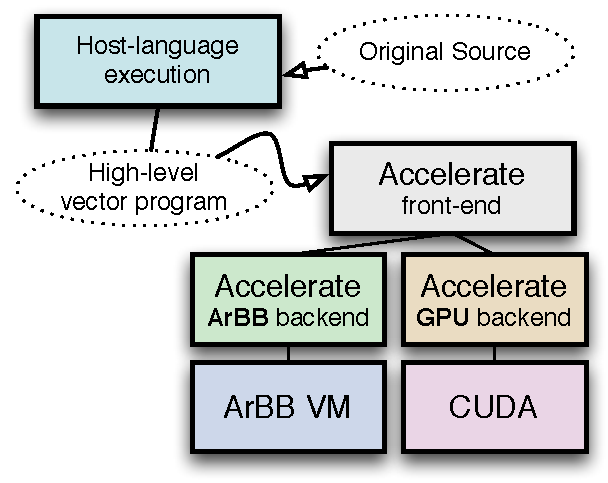
\includegraphics[width=2.0in]{./arbb/figure_architecture}    
  \end{center}
\vspace{-5mm}
  \caption{Architecture of the \systemname{} system.  \rn{(ROUGH.)}}
  \label{f:architecture}
\end{figure}


Using Accelerate and ArBB together, we propose a layered architecture
for \systemname{},
% Our goal is to make the benefits of ArBB available to the Haskell programmer. 
% \js{(Or is our goal to give an even better ``front-end'' to ArBB compared to C++)}
% We propose that this is best accomplished using a layered approach, as
pictured in Figure~\ref{f:architecture}. 
The host language execution (via Haskell in this case) executes the
programmer's source code, generating a vector program in the
restricted language of the Accelerate front-end.
Then either Accelerate backend---ArBB or CUDA---may be used.
The 
bottom layer of the ArBB backend consists of a direct mapping of the ArBB virtual machine
API (VMAPI) into Haskell including one-to-one bindings for each C 
function. 
To [partially] automate the creation of these bindings we used the C2HS system \citearbb{C2HS}. The 
\arbbvmH{} bindings are very low-level.
%and make little use of the high-level programming methods that
% Haskell programmers want. 
The idea 
is that the \arbbvmH{} bindings should be used to implement
backends for higher-level data-parallel EDSLs.

%% To illustrate our position we 
%% have started working on a backend to the successful DSL Accelerate 
%% (Data.Array.Accelerate) using our \arbbvmH{} bindings. 

To address the functionality mismatch between Accelerate and ArBB,
when possible we reencode the users Accelerate program using existing
ArBB mechanisms.  Our prototype does not support 100\% of Accelerate's
compute model (for example, only supporting  up to three-dimensional
arrays), but the remaining functionality can be mapped onto ArBB in
time using known methods---for example, our compiler could map higher
dimensional arrays onto a specific lower-dimensional data-layout.

%% The programming models supported by ArBB and Accelerate are very similar. 
%% Both obtain their parallelism by exposing collective operations 
%% such as {\em Map}, {\em Reduce}, {\em ZipWith} and {\em Scan} (all prefixes operations). However, 
%% the functionality match is not 100\%. For example, Accelerate supports {\em Map} operations 
%% over N-dimensional Arrays while ArBB supports them only up to 3-dimensions. 
%% Similar inconsistencies apply to the other operations as well. \textred{The current
%% ArBB backend simply disallows Accelerate programs using too high dimensionality
%% of the arrays.} \rn{Sure, we want to say that we're not done closing
%%   this gap (for
%%   accuracy) but more importantly we want to identify whether
%%   techniques exist to close the gap.  Presumably, yes?  We can
%%   ourselves collapse the dimensionality of arrays before giving them
%%   to ArBB?  Are there any operations that would defeat that technique?}
%

One example of a functionality discrepancy bridged by our
implementation is reductions.  As mentioned in \ref{sec:arbb},
Accelerate allows the programmer to reduce using an arbitrary
associative function, but ArBB has only built-in reductions with fixed
operations (add, multiply, xor, etc). We plan to provide general reductions in
the ArBB backend by a two-fold strategy:

\begin{enumerate}
\item Attempt to map an Accelerate reduction directly onto an ArBB
  primitive such as \cde{add\_reduce}.
\item Apply a general reduction technique based on $log(N)$ map
  operations over successively halving array sizes.  Essentially, cut
  the array in half, combine the halves, repeat. In ~\citearbb{reduction}
  this approach is explained in the context of CUDA. 
\end{enumerate}

%% \rn{Is the technique worthy of
%%   description?  Can we just cite the CUDA documentation or something
%%   since it's common?} 

In our current experiments, approach (2) is significantly slower.
Therefore, the ideal would be that ArBB exposed general reduction
directly in its programming model.  We expect this functionality to be
added in future releases.  In the meantime we plan to explore a
technique that would allow us to maximize the number of situations in
which (1) above applies.  Namely, a reduce operation can often be {\em
  factored} into a map followed by a reduce.  For example, a reduction
that multiplies each input number by a coefficient and sums the
results can be split into a map phase for the multiplication followed
by the built-in \cde {add\_reduce} operator.

%% Currently, our reduction implementations in ArBB 
%% are many times 
%% slower (\textasciitilde 20x) than their built-in counterparts. 
%% % To ameliorate this present performance problem we attempt to map
%% % programmers 
%% Our present workaround for this performance problem is to let 
%% \accarbb{} inspect the reduction function and switch to efficient 
%% built in  ArBB reduction where possible.  
%% \rn{Future work may be to decompose reductions into map+reduce so as
%%   to allow the reduce to become a builtin.}


Another choice faced by our implementation is the granularity at which the
ArBB JIT is invoked.  Specifically, should each collective operation result in its
own call to the ArBB JIT (in ArBB terminology, {\em
  immediate-mode}, akin to the pre-OpenGL 3.0 immediate mode), or
should multiple collective operations be placed together
inside an ArBB function and passed to the JIT?
We will call the latter approach {\em retained-mode}.

%% In immediate-mode the 
%% operations called from the ArBB API are executed
%% synchronously---before each API call returns. In retained-mode, ArBB
%% collects calls and, only when results are requested, the 
%% entire computation is optimized 
%% and executed. 

Retained-mode generally offers performance benefits; a bigger 
chunk is given to the JIT compiler, enabling cross-optimization
between collective operations. 
Our prototype Accelerate backend uses 
ArBB in  
a combination of immediate- and retained-mode. The main collective 
operations are compiled using the retained-mode. For example, in the case 
of a \cde{map f}  operation first the function to be mapped is created and 
compiled using retained-mode then a small {\em mapper} function is 
also created and compiled using retained-mode. 
%% The mapper function is 
%% of course very small and therefore does not give much to the JIT compiler 
%% to work on optimization-wise. 
Between the collective operations the backend
needs to perform data management and copying, which 
are performed in immediate-mode. It is our belief that 
\systemname{} would benefit from using retained-mode exclusively 
but we leave that as future work. 





% ====================================================================================================
\subsection{Preliminary Results}
% ====================================================================================================

%\rnote{One tiny benchmark if we can manage it.}

%\rnote{Ideally: Something like blackscholes running Arbb/C++,
%  \systemname{}, CPU+GPU, possibly compared to other blackscholes
%  implementations -- say Cilk on CPU and hand-coded CUDA (I can
%  provide the former I think).  Perhaps serial, non-vectorized CPU for
%  comparison.}

%\rnote{Point 1 -- High level thing is within X\% of low level thing.
%  The usual.  But we also want to say that \systemname{} is no worse
%  than ArBB/C++ -- the metalanguage doesn't matter, be it Haskell,
%  Python, or C++.}

%\rnote{Point 2 -- It's important to do a good job on the CPU side.
%  Even if you don't beat GPU there's a big difference between
%  vectorizing/not-vectorizing (and using multicore of coarse).  Can't
%  be ignored.}

%\rnote{Bonus points -- if we could show how bad ``naive'' ports are that
%  would be nice.  How well does your C CPU code run on GPU unmodified
%  (or minimally ported)?}



%\rnote{CPU/GPU systems that do a good job of both.  Perhaps quickly
%  dismiss those that make no effort on the CPU side.}

Black-Scholes option pricing is a finance-related benchmark that has been used in similar
DSLs targeting GPUs \citearbb{ACCELERATEDAMP11, NIKOLA}. Since we are re-using the 
Accelerate front-end, we can directly use the Black-Scholes benchmark that 
is shipped with that system.  Figure \ref{fig:blackscholes} shows the
complete code listing for an Accelerate Black-Scholes function which
can be executed on GPUs or any processor targeted by ArBB.

% blackscholes :: Vector (Float, Float, Float) 
%
%                -> Acc (Vector (Float, Float))
%\fbox{

%       r     = \textit{constant} riskfree
%       v     = \textit{constant} volatility

\begin{figure}
\begin{footnotesize}
\begin{Verbatim}[frame=single, commandchars=\\\{\}]
blackscholes (xs :: Vector (Float,Float,Float)) = 
  map kernel (\textit{use} xs)

kernel x =
  \kw{let} (price, strike, years) = \textit{unlift} x
      r     = 0.02 \textsf{\textit{-- riskfree constant}}
      v     = 0.30 \textsf{\textit{-- volatility constant}}
      sqrtT = sqrt years
      d1    = (log (price / strike) + 
                   (r + 0.5 * v * v) * years) / 
              (v * sqrtT)
      d2    = d1 - v * sqrtT
      cnd d = d >* 0 ? (1.0 - cndfn d, cndfn d)
      cndD1 = cnd d1
      cndD2 = cnd d2
      expRT = exp (-r * years)
  \kw{in} \textit{lift} ( price * cndD1 - 
            strike * expRT * cndD2
          , strike * expRT * (1.0 - cndD2) - 
            price * (1.0 - cndD1))

cndfn d =
  \kw{let} poly  = horner coeff
      coeff = [0, 0.31, -0.35, 1.78, -1.82, 1.33]
      rsqrt = 0.39894228040143267793994
      k     = 1.0 / (1.0 + 0.2316419 * abs d)
  \kw{in} rsqrt * exp (-0.5*d*d) * poly k

horner coeff x = 
  \kw{let} madd a b = b*x + a
  \kw{in}  foldr1 madd coeff
\end{Verbatim}
\end{footnotesize}
\caption{Complete code listing for a Black-Scholes function expressed
  in Haskell syntax using the Accelerate and \systemname{} libraries.
  Invocations of the functions \cde{use}, \cde{lift} and \cde{unlift}
%  and \cde{constant} 
represent additional boilerplate added for
  conversion in and out of Accelerate types.  Specifically, \cde{lift} and
  \cde{unlift} convert tuples and handle the fact that Accelerate
  arrays of tuples are really implemented as tuples of arrays.
  Otherwise, the program is identical to a plain Haskell
  implementation.}
\label{fig:blackscholes}
\end{figure}


%% \end{code}
%%  %605993438
%% % horner :: Num a => [a] -> a -> a
%% \begin{code}
%% \footnotesize



The kernel of this algorithm performs arithmetic on triples of
floating point numbers, creating pairs of floats as results. The problem 
is embarrassingly parallel, consisting of independent computations
for every element of an array (a map).

\begin{figure}
  \begin{center}
   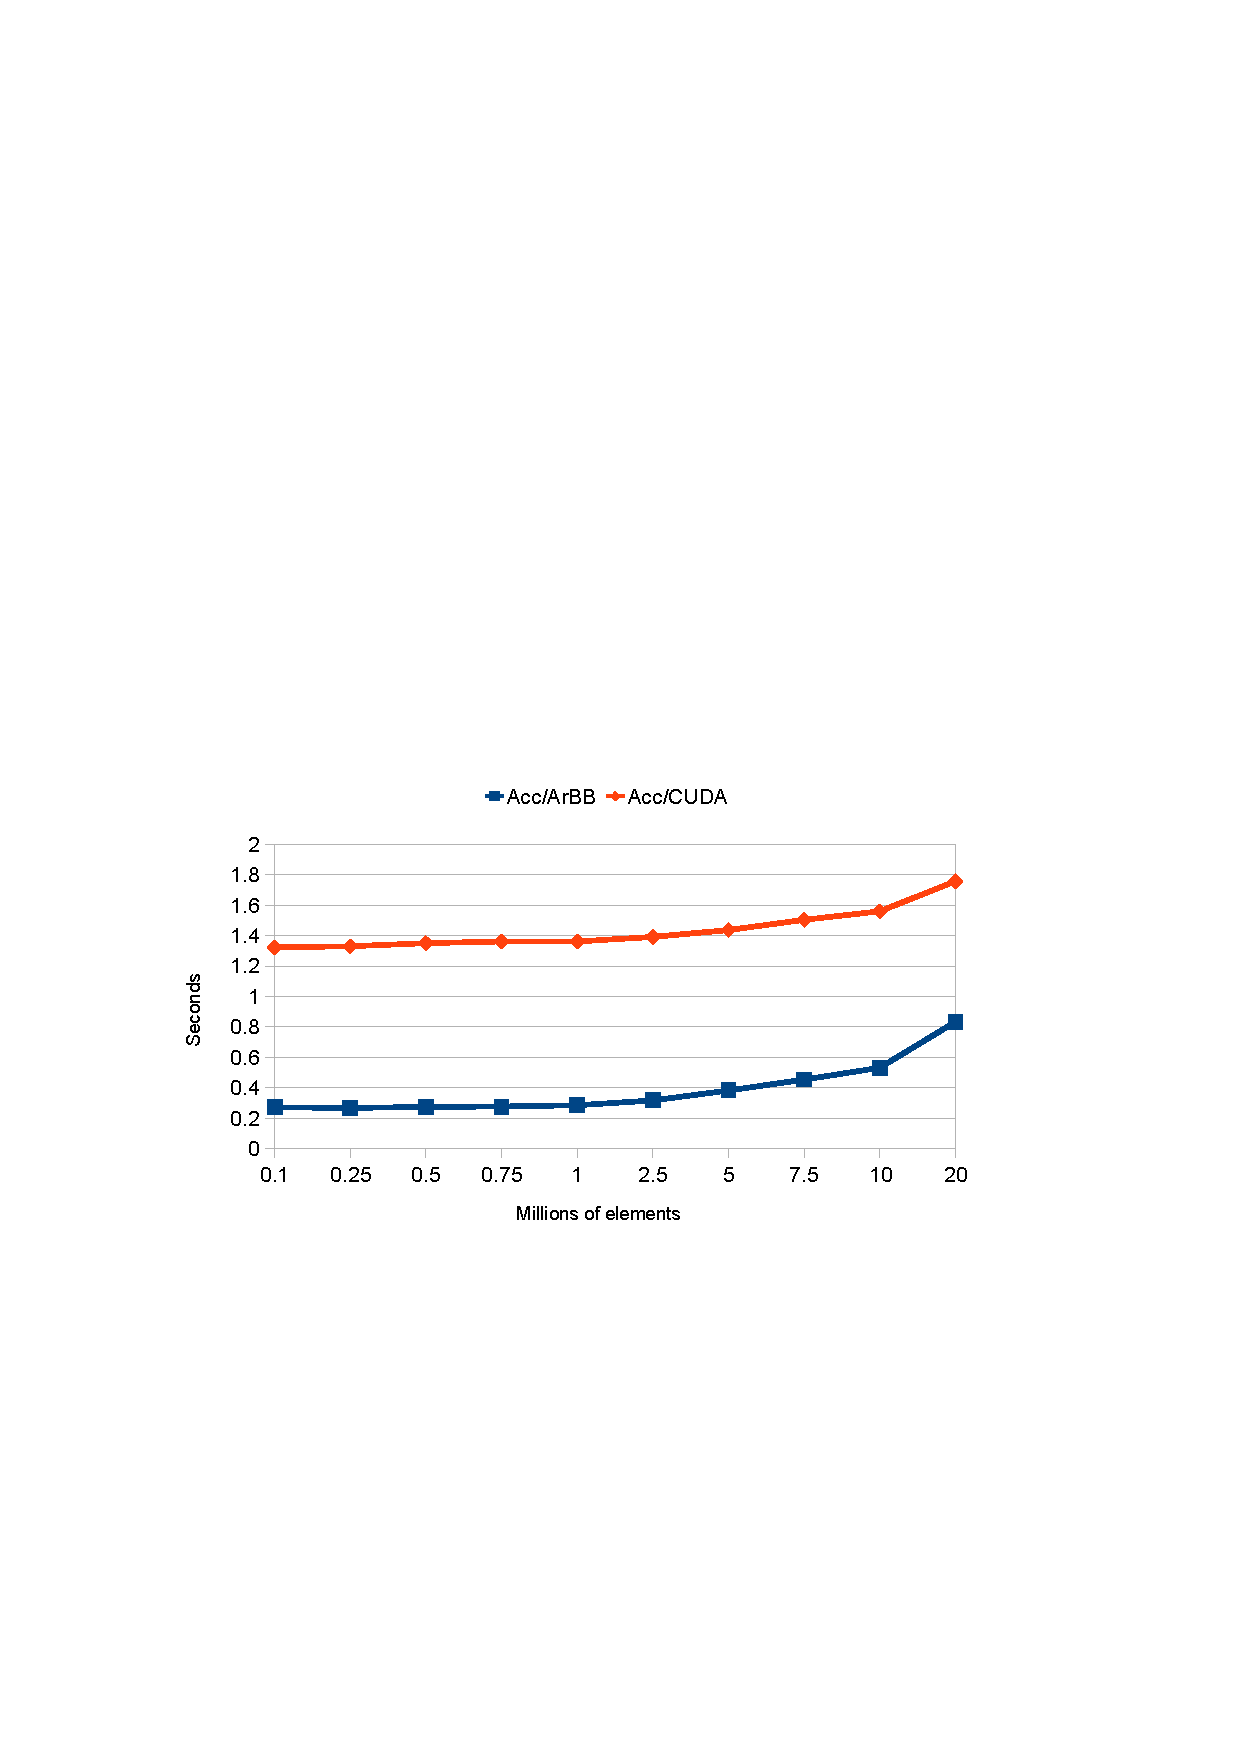
\includegraphics[width=3.5in]{./arbb/jit}    
  \end{center}
\vspace{-5mm}
  \caption{Running time experiments including JIT-time.} 
  \label{f:jit}
\end{figure}

\begin{figure}
  \begin{center}
   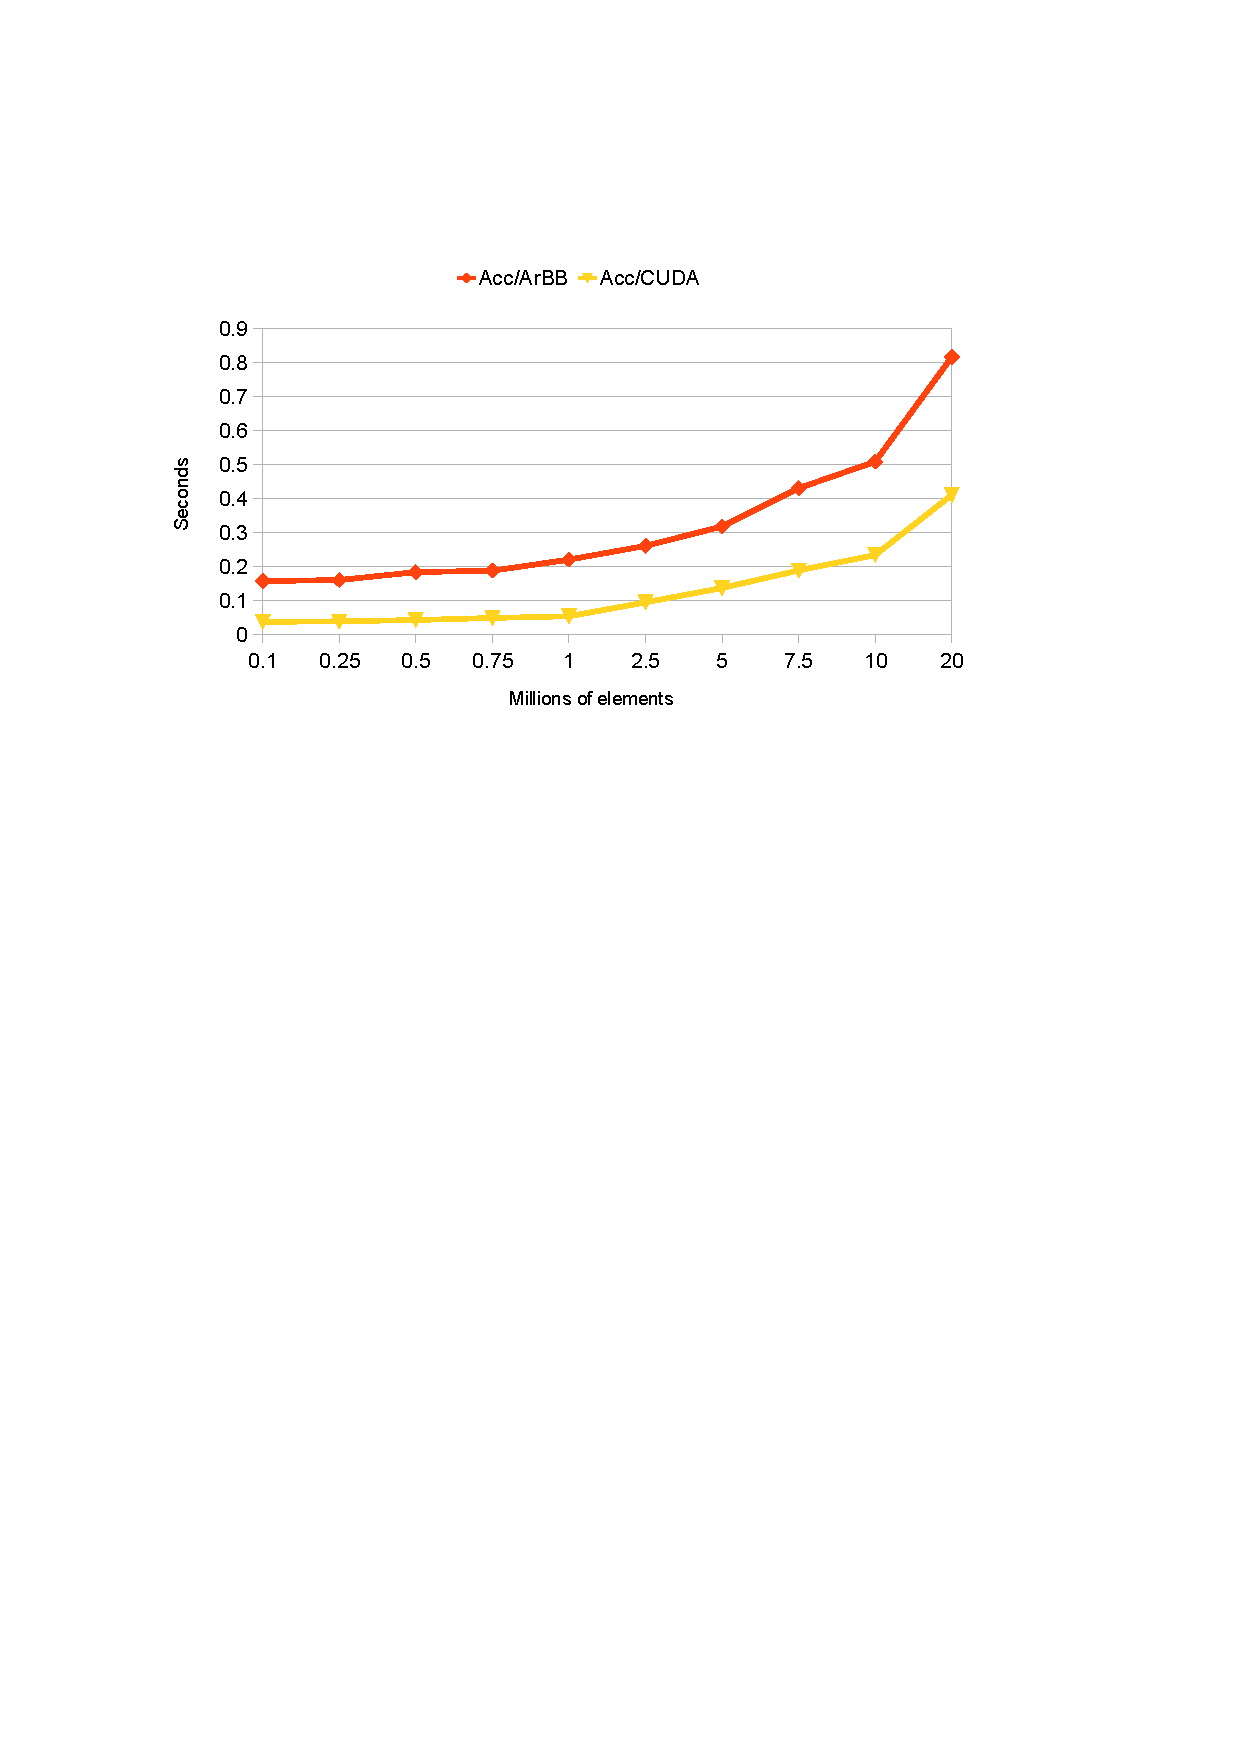
\includegraphics[width=3.5in]{./arbb/nojit}    
  \end{center}
\vspace{-5mm}
  \caption{Running time experiments JIT-time excluded.}
  \label{f:nojit}
\end{figure}


Figures~\ref{f:jit} and \ref{f:nojit} show preliminary results obtained on 
the Black-Scholes benchmark. The figures where obtained on a system with a 4-core 
Intel Core I7 975 machine with HyperThreading. The GPU used was a NVIDIA GTX480.

Figure~\ref{f:jit} shows running times obtained when JIT-time is included. 
% What this figure mainly tells us is that the JITing overhead 
JIT compilation time is much larger 
in the CUDA backend than the ArBB one.  Part of this difference 
can be attributed to the fact that 
the CUDA backend calls an external compiler (\cde{nvcc}), which takes its input in a file and runs in
a separate process.  ArBB, on the other hand, has a library interface to its  JIT-compiler. 
Figure~\ref{f:nojit} shows results obtained when pre-compiling the
CUDA functions eliminating JIT overhead.
In Accelerate, this happens automatically when the same kernel is
invoked repeatedly, because the Accelerate CUDA backed 
uses a caching scheme to avoid unnecessary JIT invocations.  (The
caching functionality has not yet been duplicated in the 
ArBB backend.)

These early results demonstrates the principle that even when a kernel
executes with higher throughput on a GPU, in a particular program it
is difficult to decide whether a computation is worth moving to a GPU,
incurring extra data-movement and possibly extra JIT compilation
\citearbb{wheres-the-data-paper}.  Specifically, we see that the
Accelerate Black-Scholes program from Figure~\ref{fig:blackscholes}
performs better on the CPU if it executes once (even on a large window
of data) whereas the GPU would yield better performance in a sustained
series of executions.
%
Because both CPU and GPU execution may be desirable---and the
selection may be dynamic---it is beneficial to have a single source code
that is portable across both.  
% Accelerate combined with \systemname{} makes this possible.


% ====================================================================================================
\subsection{Related Work}
% ====================================================================================================


OpenCL~\citearbb{opencl08} is a programming model very similar to CUDA but with the aspiration 
to offer both acceleration of computations on GPUs or to multicore CPUs. 
OpenCL JIT compiles the kernels for the particular hardware available and is
in that sense similar to ArBB.  
OpenCL programs are relatively low-level and require a large amount of
boilerplate to create and invoke.  In this sense they occupy a very
different niche than Accelerate.

Microsoft Accelerator~\citearbb{ACCELERATOR} is an embedded language with similar 
aspirations as ArBB, that is, to target a diverse range of architectures using the 
same source code. Accelerate can be used from the C\# language or the 
functional F\# language and targets GPUs or of CPUs and their
vector units.
% However, being part of the .Net framework implies limited accessibility 
%for platforms other than Microsoft Windows.  

\rn{What's the comparison with our stuff?}

%Most work on partitioning workloads between 
Many CPU and GPU comparisons, and some CPU/GPU workload partitioners \citearbb{merge}, rely on
redundant hand-written versions of all kernels
% \citearbb{cpu-gpu-partitioning} 
(though some systems like Qilin \citearbb{qilin} allow a single source code).
It is difficult in this kind of scenario
to make fair comparisons, controlling for the
amount of effort put into the respective implementations.
For example, comparing unoptimized serial CPU implementations vs. GPU
ones is not informative \citearbb{debunking-dubey}.
In \systemname{} controlling for effort
need happen only once---both CUDA and ArBB are
independently optimized by their respective teams of engineers---not for each benchmark.


% ====================================================================================================
% \section{Future work and Conclusions}
%\section{Future Work}
% ====================================================================================================

%\rn{need to be careful about being too repetitive...}
%The \accarbb{} backend is currently work-in-progress. The Accelerate
%functionality is not yet completely covered by the ArBB backend. Currently 
%the ArBB back-ed is operational for Accelerate programs using {\em Map}, 
%{\em ZipWith} and some simple instances of the Accelerate {\em Fold} operation.
%All of these also have the limitation that they only work for up to and 
%including 3-dimensional arrays using the ArBB backend while the Accelerate
%model allows the N-dimensional case. Allowing the N-dimensional case 
%in the ArBB backend for the supported operations range from a simple exercise 
%to more intricate problems needing some thought. For example, in the case 
%{\em Map} operations the needed transformation is simple (Accelerate Maps 
%over N-dimensional arrays is a per-element operation). One could flatten 
%the N-dimensional array to a 1-dimensional array (remembering its old shape) 
%perform the map and then transform the array back into N-dimensions. In 
%the case of {\em Fold} (reductions) the situation becomes more tricky. 
%transforming the arrays to arrays of lesser dimensionality then requires 
%a so-called segmented {\em Fold} operation. 

%The current \accarbb{} backend uses a hybrid of immediate-mode 
%and retained-mode programming styles. Moving more towards 
%retained-mode only may have performance benefits since it would give the 
%ArBB compiler larger programs to optimize. Exploring this aspect is left 
%as future work. 

% ====================================================================================================
\subsection{Discussion and Conclusions}
% ====================================================================================================

We have demonstrated that an EDSL such as Accelerate is sufficiently
platform-independent to break free of its original hardware target
(CUDA/GPU) and create efficient programs on other architectures.  This
gives us hope that \systemname{}/Accelerate programs will be
forward-portable to future parallel architectures and instruction
sets.

The EDSL approach changes the playing field for the designer
of compiler backends.  Rather than contending with full blown
languages and their complexities (e.g. pointers, aliasing,
inheritance, virtual functions, etc), compiler backends can focus on
simple value-oriented compute languages.

%% Achieving the ultimate goal of performance portability requires
%% progress on two research problems.  The first is EDSLs themselves and
%% their integration into host languages.  The second problem 

But the EDSL method solves only part of the performance-portability problem.
Simple as EDSL target languages may be, there remains a
substantial challenge in mapping them efficiently to the diversity
of parallel architectures available now and in the near future.
%especially without requiring a large amount of additional per-platform
%user annotations.
\textred{For example, the idiosyncrasies of memory bank access on
  NVIDIA GPUs must be taken into account to generate efficient
  implementations of the high-level collective operations that we have
  discussed.}

This is a compiler backend research challenge.
The {\em skeletons} method mentioned in
Section~\ref{sec:accelerate-arbb} is one approach to this problem, as
are the optimizations studied in the Copperhead \citearbb{copperhead} and
Obsidian \citearbb{JSLIC} projects.
%
On the other hand, systems that rely on advanced optimizations
typically suffer to some extent from performance-predictability
problems.  Thus achieving portable, predictable performance on a wide range
of architectures---even for the simplest target languages---will
be the subject of much future work.

%{
%\small
\bibliographystylearbb{alpha}
\bibliographyarbb{thesis}
%}


%\end{document}




% ---------------------------------------------------------------------------
% 
% ---------------------------------------------------------------------------
\cleardoublepage 

\section[\paperCTitle]{\paperC: \\ \paperCTitle}
\label{sec:paperC}
%\addcontentsline{toc}{chapter}{Obsidian: GPU Computing Using Haskell}

%\paperCTitle

\begin{center} 
Bo Joel Svensson, Koen Claessen, Mary Sheeran
\end{center}


%% bare_conf.tex
%% V1.3
%% 2007/01/11
%% by Michael Shell
%% See:
%% http://www.michaelshell.org/
%% for current contact information.
%%
%% This is a skeleton file demonstrating the use of IEEEtran.cls
%% (requires IEEEtran.cls version 1.7 or later) with an IEEE conference paper.
%%
%% Support sites:
%% http://www.michaelshell.org/tex/ieeetran/
%% http://www.ctan.org/tex-archive/macros/latex/contrib/IEEEtran/
%% and
%% http://www.ieee.org/

%\documentclass[conference]{IEEEtran}

%\usepackage{graphicx, color, code}
%\usepackage[cmex10]{amsmath}
%\usepackage{url}
% \usepackage{bookman}  %% bold teletype fonts, but don't know how to prevent it from changing the whole document

% Haven't figured out how to get this to work properly:
%\usepackage[\texttt{cmbtt}]{bold-extra}
% \usepackage{bold-extra} 

%\usepackage{courier}
%\usepackage{fancyvrb}

% correct bad hyphenation here
%\hyphenation{op-tical net-works semi-conduc-tor}


%====================================================================================================
%% FIRST, MISC USEFUL DEFINITIONS
%====================================================================================================

\definecolor{darkgreen}{rgb}{0, 0.5, 0}
\definecolor{darkblue}{rgb}{0,0,0.5}
\definecolor{mygrey}{rgb}{0.7,0.7,0.7}
\newcommand{\textblue}[1]{\textcolor{blue}{#1}}

\newcommand{\cde}[1]{{\footnotesize \tt #1}}

% \newcommand{\kw}[1]{{\bf{#1}}}
\newcommand{\kw}[1]{{\textbf{#1}}}

\newcommand{\comm}[1]{{\em \textcolor{darkgreen}{#1}}}  %% Code comments

\newcommand{\note}[1]{\begin{itemize}\item \textcolor{blue}{#1} \end{itemize}}

%% \newenvironment{mycode}
%% {% This is the begin code
%%   \begin{Verbatim}[commandchars=\\\{\}]}%
%%   %\footnotesize
%%   %\noindent
%%   %\begin{code}\noindent\vspace{-1mm}}
%% %  \begin{code}\noindent}
%% {% This is the end code
%%   \end{Verbatim}
%%   %\end{code} 
%% }

%% \newenvironment{inlinecode}
%% {
%%   \begin{center}
%%   \begin{minipage}{4in}
%%   \begin{mycode}
%% } 
%% {
%%   \end{mycode}
%%   \end{minipage}
%%   \end{center}
%%   \vspace{-1.5ex}
%% }

%% ============================================================
%% USE TO DISABLE COMMENTS:
 \def\noeditingmarks{}
%% ============================================================
\ifx\noeditingmarks\undefined
   \newcommand{\textred}[1]{\textcolor{red}{#1}}
   \newcommand{\pgwrapper}[2]{\textred{#1: #2}}
%   \newcommand{\pgwrapper}[2]{}
   \newcommand{\rnote}[1]{\begin{itemize}\item{\textcolor{blue}{#1}}\end{itemize}}
   \newcommand{\new}[1]{\textcolor{blue}{#1}}
   \newcommand{\const}[1]{\textred{#1}}

%% RRN: Dim the background for Ryan's eyes:
%%   What I need here is a way to do it based on user or host name...
% \pagecolor{mygrey}

\else
   \newcommand{\textred}[1]{#1}
   \newcommand{\pgwrapper}[2]{}
   \newcommand{\rnote}[1]{}
   \newcommand{\new}[1]{#1}
   \newcommand{\const}[1]{#1}
\fi

\newcommand{\js}[1]{\pgwrapper{BJS}{#1}}
\newcommand{\rn}[1]{\pgwrapper{RRN}{#1}}


%% Can we call our ``things'' 
%% ArBB/Haskell for the bindings part ? 
%% Accelerate/ArBB for the Accelerate backend ?
%% This would work with the convention we adopted for 
%%      ArBB/C++  
\newcommand{\systemname}[0]{{Harbb}}
%\newcommand{\systemname}[0]{\textred{HArBB}}

%% This could in theory be separate from the project name..
\newcommand{\accarbb}[0]{\systemname{}}

%% NOTE: THIS SHOULD BE THE SAME AS SYSTEMNAME:
\newcommand{\arbbvmH}[0]{ArBB/Haskell}


%====================================================================================================
% END DEFINITIONS
%====================================================================================================




%\begin{document}
% \title{Painless Portable Vector Parallelism\\ with Haskell and Intel ArBB}
%\title{Programming Future Parallel Architectures\\ with Haskell and Intel ArBB}
% \title{Embedded Domain-Specific Languages Pave the Way for New Parallel Architectures}

%\author{\IEEEauthorblockN{Bo Joel Svensson}
%\IEEEauthorblockA{Dept. of Computer Science and Engineering\\
%Chalmers University of Technology\\
%Gothenburg, Sweden\\
%Email: joels@chalmers.se}
%\and
%\IEEEauthorblockN{Ryan Newton}
%\IEEEauthorblockA{Intel Corporation\\
%Hudson, MA\\
%Email: rrnewton@gmail.com
%}}
% Email: ryan.r.newton@intel.com

%\maketitle

%\begin{abstract}
%
\subsection*{Abstract}
New parallel architectures, such 
\new{as Cell, Intel MIC, GPUs, and tiled architectures, enable} high
performance but are often hard to program.
What is needed is a bridge between high-level programming models 
where programmers are most productive and modern parallel architectures. 
We propose that that bridge is Embedded Domain Specific Languages (EDSLs). 

\new{One attractive target for EDSLs is}
Intel ArBB, a virtual machine for parallel, vectorized computations.
% that serves as a compilation target for EDSLs.
We propose to wed ArBB with the functional programming language
Haskell, {using an EDSL} that generates code for the ArBB VM.  This Haskell integration provides 
% a determinism guarantee 
added safety guarantees compared to other ArBB interfaces.
%
Further, our prototype, \systemname{}, is one of the first EDSL implementations with
optimized backends for multiple parallel architectures (CPU, \new{NVIDIA GPU}, and
others), allowing portability of source code over devices
and their accelerators.


%\end{abstract}
%\IEEEpeerreviewmaketitle




% ====================================================================================================
\subsection{Introduction}
% ====================================================================================================

Are radical new parallel architectures market-feasible if they require
significant changes for programmers?  The jury is out.  In recent
years we have seen difficult-to-program chips suffer 
% \citearbb{cell} 
(e.g. Cell)
and
GPU vendors strive to enable more traditional programming features
\citearbb{fermi} (e.g. C++).  There is an increasing
tension between ease of programming and efficiency.

The tension  shows  across diverse chip markets.  For example,
small embedded devices are most power efficient if their processors and operating systems
omit programming features such as virtual memory and threads \citearbb{tinyos}.  
At the other end of the power spectrum, GPU's
graphics performance may suffer due to inclusion of hardware to ease
GPGPU programming.  In short, there is an opportunity cost to
including extra hardware for programmability.

In this paper, we argue 
that a specific technique holds the greatest promise of solving the programmability dilemma.
%
Domain-specific languages, {\em embedded} within general purpose
languages (EDSLs) 
 enable familiar programming models 
{\em and} flexible
mapping onto new hardware.  The key to having this cake and eating it
too is {\em metaprogramming}.  Familiar programming features are
present, but are eliminated at an intermediate (metaprogram evaluation)
phase and therefore do not reach the parallel hardware itself.


% We present our ongoing work on a
In pursuit of this vision, we offer a
% 
 new EDSL implementation, called \accarbb{}, that combines
existing systems, Accelerate \citearbb{ACCELERATEDAMP11} and ArBB \citearbb{ArBB}, to produce a unified
high-level programming environment equally suited to multicore,
vectorized CPUs, as to GPUs and other accelerators (such as Intel MIC chips \citearbb{larrabee}).
%
\if{0}
ArBB is based on the RapidMind \citearbb{RapidMind} system which was an embedded 
DSL targeting multicore CPUs as well as GPUs. ArBB does not \new{yet} include a GPU 
backend like RapidMind, targeting multicore CPUs and their vector 
units. 
\fi{}
\systemname{} is a single EDSL implementation 
with independently optimized backends \new{by different teams; 
namely, the ArBB backend for CPU/MIC, and a CUDA backend for NVIDIA GPU.}
This makes
\systemname{} an appealing platform for fair CPU/GPU comparisons, 
as well as a compelling programming model for single-source portable performance across a range of
parallel architectures, \new{present and future}.
%%To our knowledge, \systemname{} is the first EDSL implementation with
%%independently optimized backends for CPUs and GPUs.  This makes
%%\systemname{} an appealing platform for fair CPU/GPU comparisons, 
%%as well as a compelling programming
%%model for single-source portable performance across a range of
%%parallel architectures.


% ====================================================================================================
\subsection{Embedded Domain-Specific Languages}
% ====================================================================================================


Domain-specific languages---from Makefiles and \LaTeX{} to
Matlab---are almost too ubiquitous to notice.  Most relevant to our
purposes, domain-specific languages (DSLs) that target a narrow domain and expose communication
patterns to the compiler 
 have achieved performance-portability across a wide range of parallel
architectures.  
StreamIt\citearbb{streamit} is a good example.
% (for example, StreamIt\citearbb{streamit})
% The high-water mark in this area is perhaps  StreamIt\citearbb{streamit}.
% 

% It has been noted \citearbb{not-sure} that 
% Yet the few DSLs that gain popularity lose simplicity\citearbb{not-sure}.  
% Yet popular DSLs rarely remain simple \citearbb{not-sure}.  
DSLs may start out simple and focused, but if they gain popularity
they quickly grow in complexity to rival full-blown languages.
Feature creep
can make DSL implementations complex and expensive to maintain.
Further, non-standard DSL syntax and features present a learning curve for users.  In the
last ten years an attractive solution to this dilemma has emerged: {\em
  embed} each DSL into a general-purpose host language that can provide
common functionality with familiar syntax and semantics.
% in place of the DSL.

When embedding, host language programs {generate} DSL programs;
% Embedding means that the host language is used to generate DSL programs; 
the {\em deeper} the embedding, the more integrated the
DSL into the syntax and type-system of the host language.
%
% Typically, %% pruning weasel words
A key host-language feature for embedding is that
language constructs can be overloaded to operate over {\em abstract
  syntax trees} (ASTs)\footnote{This ad-hoc polymorphism is accomplished,
for example, through operator-overloading in C++ or type classes in
Haskell.}.  For example, the following simple function operates on scalars:


\vspace{1mm}
\begin{Verbatim}[commandchars=\\\{\}]
  float f(float x) \{ return (2*x - 1); \}
\end{Verbatim}
\noindent
But simply by changing the types, \cde{f} might be lifted to operate on {\em
  expressions} (which, when evaluated, will yield \cde{floats}):

\vspace{1mm}
\begin{Verbatim}[commandchars=\\\{\}]
  \kw{exp<float>} f(\kw{exp<float>} x) \{
    return (2*x - 1);
  \}
\end{Verbatim}

A common arrangement is for the host language program to execute at
runtime but to generate ASTs that are executed by a just-in-time
(DSL) compiler.  This use of metaprogramming (program generation)
differs from the more common usage of preprocessors and 
% Lisp/Scheme macros \citearbb{scheme-macros}
macros, which typically add extra
phases of computation {\em before}  compile time---increasing
the number of compile-time rather than runtime phases.

% EDSLs typically add additional runtime phases.  That is, the host language program 
% executes at runtime but uses a JIT to process generated ASTs.
%% which are
%% usually used to perform computation {\em earlier} than the usual
%% compile time, embedded DSLs (EDSLs) typically defer computation 


One reason that EDSLs are good for productivity is that the programmer
gains the software engineering benefits of the host language
(object-orientation, higher-order-functions, modules, etc), while not
paying the cost at runtime for additional layers of abstraction or
indirection.  Indeed, the embedded languages for 
performance-oriented EDSLs are often simple, first-order
languages without pointers \citearbb{wavescript, ACCELERATEDAMP11}.

% , paul-lius-thingy

% regiment,
As a research area, EDSLs and two-stage DSLs have been actively pursued for at least a
decade \citearbb{VERTIGO, wavescript} but are gaining steam
recently 
%\citearbb{sejits, stanford-ppl} 
\citearbb{copperhead, stanford-ppl} 
and are beginning to appear in
commercial products \citearbb{ArBB}.
%
Further, EDSL techniques have spread beyond their origin in 
 the programming languages community.
% 
For example, both Stanford's Parallel Programming Laboratory (PPL) and
the Berkeley Parlab are creating EDSLs as their flagship parallel
programming solutions for domains such as machine learning and
rendering \citearbb{stanford-ppl}.
  Moreover, EDSLs need not be hosted by esoteric research languages---Intel's
 ArBB embeds an array language in C++ and Berkeley's
Copperhead \citearbb{copperhead} generates CUDA from simple Python code.

%\rnote{Is there a good motivating example program?  What are some of
%  the Metaocaml motivating examples?}

{For the remainder of this paper we will focus our discussion
  on the Intel ArBB VM, a virtual machine for just-in-time
  generation of vector codes, \new{which implements a restricted} domain-specific
  language of array computations.  In this paper we introduce
  {\em High-level ArBB}, 
  (\systemname{}), an EDSL that internally uses the ArBB
  VM.  \new{While Intel's ArBB package already includes an EDSL targeting the VM (for C++)},
\systemname{} \new{offers additional advantages, including}
  more succinct programs and additionally safety
  guarantees---namely, complete deterministic-by-construction parallel
  programs (across both host and VM languages).}


% ====================================================================================================
% \section{Accelerate and ArBB}
%\section{\accarbb{}:  ArBB and Accelerate}
\subsection{\accarbb{} $=$ ArBB $+$ Accelerate}
\label{sec:accelerate-arbb}
% ====================================================================================================

Our first \systemname{} prototype adapts an existing EDSL called {\em
  Accelerate} (Data.Array.Accelerate).  Accelerate targets high-level
data-parallel programming in Haskell.
Previous work on Accelerate has focused on developing a CUDA-backend
for GPU programming.  In this paper we describe our effort to retarget
Accelerate to ArBB.  

With respect to determinism guarantees, the existing Intel ArBB product
represents an integration of the safe (ArBB VM) with the unsafe (C++).
In the Haskell context, because purely functional computations are
guaranteed deterministic (even when executed in parallel), and because
ArBB computations invoked by Haskell functions are themselves free of
side-effects, \systemname{} achieves a
guarantee of determinism for complete programs that combine both
Haskell computation and ArBB VM computation.
% which offers portability.
% (The 'H' in \systemname{} therefore stands for Haskell as well as ``High-level''.)


%% {\em Accelerate} (Data.Array.Accelerate) is an existing EDSL for 
%% high-level data-parallel programming in Haskell~\citearbb{Accelerate}. 
The Accelerate programming model consists of collective 
operations that can be performed over arrays, together with a simple 
language of scalar expressions\new{---in the current release, the Haskell type system enforces that parallelism not be nested.}
\if{0}
The Haskell type 
system is used to enforce that no nested data-parallelism can be expressed 
\new{(in the current release, this may be relaxed in the future).}
\fi{}
Accelerate's collective operations include {\em Map} (akin to parallel
for loops) {\em ZipWith} (a generalization of elementwise vector addition) and 
{\em Fold} (sum generalized)---familiar operations for programmers versed in the functional paradigm.
All of these collective operations are easily parallelizable. 
% In the case of {\em Map} and {\em ZipWith} the potential for parallelism is abundant.  

%% dotProd :: Vector Float -> 
%%            Vector Float -> 
%%            Acc (Scalar Float) 
\begin{Verbatim}[commandchars=\\\{\}]
dotProd (xs :: Vector Float) 
        (ys :: Vector Float) = 
  \kw{let} xs\_ = use xs 
      ys\_ = use ys 
  \kw{in}  fold (+) 0 (zipWith (*) xs\_ ys\_) 
\end{Verbatim}

The Accelerate code listing above specifies a function that takes two 1-dimensional 
arrays as inputs (of type \cde{Vector Float}, e.g. a vector of floats). The result of the function is a single
scalar. 
% (\cde{Scalar Float})
The \cde{use} function is applied to an array to convert it 
for use in the collective operations provided by Accelerate;
\cde{use} 
% is actually a function with type \cde{Vector a -> Acc (Vector a)} and 
may result in
copying the array to, for example, the GPU in the case of Accelerate's 
CUDA backend.  

After applying \cde{use} to bring in input data, the programmer then
constructs a data-parallel program from collective operations.
Above, \cde{fold} is a function that takes three arguments, 
here those arguments are \cde{(+)},  $0$ and \cde{zipWith (*) xs\_ ys\_}. 
\cde{zipWith}, in turn, is a function taking three arguments, \cde{(*)}, 
\cde{xs\_} and \cde{ys\_}. The \cde{zipWith} operation here applies pairwise 
multiplication to the two arrays and the \cde{fold} sums up all the elements 
into a single scalar. 

%\rn{Following para slightly redundant but ok...}
%Accelerate makes GPU programming accessible to the functional programmer 
%by offering a familiar set of operations. This set of operations also have 
%the beneficial property that they have inherent parallelism and are 
%easily implementable on the GPU. 

Accelerate's CUDA backend implements collective operations using
a hand-tuned ``skeleton'' for each operation (and possibly for
different hardware versions). The kernel---for example, the function
to mapped over the dataset---is 
instantiated into the body of the skeleton code. The resulting 
program is compiled using the NVIDIA CUDA compiler and dynamically linked 
into the running Haskell program.

%\subsection{Intel Array Building Blocks (ArBB)}
\subsection{Intel Array Building Blocks (ArBB)}
\label{sec:arbb}

%ArBB is embedded in the C++ programming language but it also exposes a 
%very low level API that is purely C. 
%{\em ArBB} (Array Building Blocks) is also an embedded DSL. 
The operations exposed by ArBB are similar to those of Accelerate. 
In ArBB, parallel computations are expressed using a set of built-in 
primitives. All vectorization and threading is managed internally by 
ArBB. The programmer uses collective operations with a clear semantics 
such as \cde {add\_reduce} that computes the sum of the elements in a given 
array. ArBB also has language constructions for control flow, conditionals
and loops. These operations have their usual sequential semantics and are not 
parallelized by the system, rather, only specific collective operations are executed
in parallel. 

Today's existing ArBB product is embedded in C++ and provides special
types for scalars and arrays (e.g. \cde{dense<f32>} rather than \cde{vector<float>}).
Using ArBB/C++ to express the dot product computation can be done 
as follows:

%\vspace{2mm}
\begin{Verbatim}[commandchars=\\\{\}]
\kw{void} dot\_product(\kw{const} dense<f32>& a, 
                 \kw{const} dense<f32>& b,
                 f32& c) 
{ 
  c = add\_reduce(a * b);
}
\end{Verbatim} 


% The above program takes two arrays of type \cde{dense<f32>} as input. 
% \cde{dense<f32>} specifies a 1-dimensional array of 32-bit floating
% point values. The result is a single 32-bit float.  

Note that arithmetic operators such as (*) are overloaded 
for to operate on arrays as well as scalars (e.g. \cde{a * b} above).
Thus, the above C++ function multiplies two arrays before summing them with \cde {add\_reduce}:

The code listing below is indicative to the amount of glue code needed to invoke an 
ArBB computation\footnote{In OpenCL and CUDA the glue code situation is even worse}. It shows how the dot product code is launched using {\tt call} and 
how data is bound, {\tt bind}, for use in ArBB. 

\vspace{2mm}
\begin{Verbatim}[commandchars=\\\{\}]
\kw{int} main() 
\{ 
  double a[SIZE];
  double b[SIZE];

  for ( \kw{int} i = 0; i < SIZE; ++i) \{ 
    a[i] = ...; b[i] = ...;
  \}
  dense<f32> va, vb;
  f32 vc;
  bind(va, a, SIZE); 
  bind(vb, b, SIZE); 
  call(dot\_product)(va, vb, &vc); 
  ...
\}
\end{Verbatim}


%\rnote{SPECIFICALLY ADDRESS THE FUNCTIONALITY GAP?  E.G general
%  reduce.  Any other examples?}

The model provided by Accelerate is slightly richer than that of ArBB.
Even the two very simple \cde {dot\_product} examples above manage to illustrate 
this. In Accelerate there is a more general reduction primitive called \cde {fold} 
where in ArBB there are specific reductions, \cde {add\_reduce}, \cde {mul\_reduce} 
and so on. Not visible in these small examples is another difference, Accelerate 
operations are generalized to arbitrary dimensions while ArBB operations are 
limited to 1, 2, and 3 dimensions (and 0, i.e. scalar). These differences aside,
the ArBB and Accelerate programming models are very similar.


% ====================================================================================================
\subsection{Implementation of \systemname{}} 
% ====================================================================================================


%\rnote{Sadly the Haskell details don't buy us much here... what are
%  the {\em conceptual} problems solved in mapping the Accelerate
%  abstraction to the ArBB one?  The data models are similar, but
%  there are always mismatches -- dimensionality support, missing
%  reduction.}

%\rnote{What is the technique that you are using to address these sorts
%  of problems?  Is there anything to say about it?}

\begin{figure}
  \begin{center}
   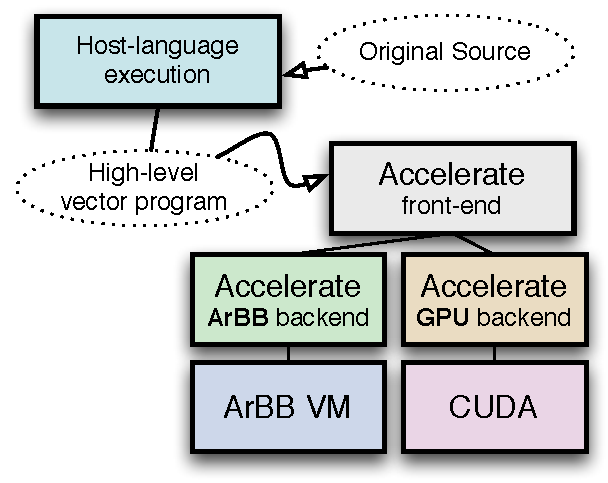
\includegraphics[width=2.0in]{./arbb/figure_architecture}    
  \end{center}
\vspace{-5mm}
  \caption{Architecture of the \systemname{} system.  \rn{(ROUGH.)}}
  \label{f:architecture}
\end{figure}


Using Accelerate and ArBB together, we propose a layered architecture
for \systemname{},
% Our goal is to make the benefits of ArBB available to the Haskell programmer. 
% \js{(Or is our goal to give an even better ``front-end'' to ArBB compared to C++)}
% We propose that this is best accomplished using a layered approach, as
pictured in Figure~\ref{f:architecture}. 
The host language execution (via Haskell in this case) executes the
programmer's source code, generating a vector program in the
restricted language of the Accelerate front-end.
Then either Accelerate backend---ArBB or CUDA---may be used.
The 
bottom layer of the ArBB backend consists of a direct mapping of the ArBB virtual machine
API (VMAPI) into Haskell including one-to-one bindings for each C 
function. 
To [partially] automate the creation of these bindings we used the C2HS system \citearbb{C2HS}. The 
\arbbvmH{} bindings are very low-level.
%and make little use of the high-level programming methods that
% Haskell programmers want. 
The idea 
is that the \arbbvmH{} bindings should be used to implement
backends for higher-level data-parallel EDSLs.

%% To illustrate our position we 
%% have started working on a backend to the successful DSL Accelerate 
%% (Data.Array.Accelerate) using our \arbbvmH{} bindings. 

To address the functionality mismatch between Accelerate and ArBB,
when possible we reencode the users Accelerate program using existing
ArBB mechanisms.  Our prototype does not support 100\% of Accelerate's
compute model (for example, only supporting  up to three-dimensional
arrays), but the remaining functionality can be mapped onto ArBB in
time using known methods---for example, our compiler could map higher
dimensional arrays onto a specific lower-dimensional data-layout.

%% The programming models supported by ArBB and Accelerate are very similar. 
%% Both obtain their parallelism by exposing collective operations 
%% such as {\em Map}, {\em Reduce}, {\em ZipWith} and {\em Scan} (all prefixes operations). However, 
%% the functionality match is not 100\%. For example, Accelerate supports {\em Map} operations 
%% over N-dimensional Arrays while ArBB supports them only up to 3-dimensions. 
%% Similar inconsistencies apply to the other operations as well. \textred{The current
%% ArBB backend simply disallows Accelerate programs using too high dimensionality
%% of the arrays.} \rn{Sure, we want to say that we're not done closing
%%   this gap (for
%%   accuracy) but more importantly we want to identify whether
%%   techniques exist to close the gap.  Presumably, yes?  We can
%%   ourselves collapse the dimensionality of arrays before giving them
%%   to ArBB?  Are there any operations that would defeat that technique?}
%

One example of a functionality discrepancy bridged by our
implementation is reductions.  As mentioned in \ref{sec:arbb},
Accelerate allows the programmer to reduce using an arbitrary
associative function, but ArBB has only built-in reductions with fixed
operations (add, multiply, xor, etc). We plan to provide general reductions in
the ArBB backend by a two-fold strategy:

\begin{enumerate}
\item Attempt to map an Accelerate reduction directly onto an ArBB
  primitive such as \cde{add\_reduce}.
\item Apply a general reduction technique based on $log(N)$ map
  operations over successively halving array sizes.  Essentially, cut
  the array in half, combine the halves, repeat. In ~\citearbb{reduction}
  this approach is explained in the context of CUDA. 
\end{enumerate}

%% \rn{Is the technique worthy of
%%   description?  Can we just cite the CUDA documentation or something
%%   since it's common?} 

In our current experiments, approach (2) is significantly slower.
Therefore, the ideal would be that ArBB exposed general reduction
directly in its programming model.  We expect this functionality to be
added in future releases.  In the meantime we plan to explore a
technique that would allow us to maximize the number of situations in
which (1) above applies.  Namely, a reduce operation can often be {\em
  factored} into a map followed by a reduce.  For example, a reduction
that multiplies each input number by a coefficient and sums the
results can be split into a map phase for the multiplication followed
by the built-in \cde {add\_reduce} operator.

%% Currently, our reduction implementations in ArBB 
%% are many times 
%% slower (\textasciitilde 20x) than their built-in counterparts. 
%% % To ameliorate this present performance problem we attempt to map
%% % programmers 
%% Our present workaround for this performance problem is to let 
%% \accarbb{} inspect the reduction function and switch to efficient 
%% built in  ArBB reduction where possible.  
%% \rn{Future work may be to decompose reductions into map+reduce so as
%%   to allow the reduce to become a builtin.}


Another choice faced by our implementation is the granularity at which the
ArBB JIT is invoked.  Specifically, should each collective operation result in its
own call to the ArBB JIT (in ArBB terminology, {\em
  immediate-mode}, akin to the pre-OpenGL 3.0 immediate mode), or
should multiple collective operations be placed together
inside an ArBB function and passed to the JIT?
We will call the latter approach {\em retained-mode}.

%% In immediate-mode the 
%% operations called from the ArBB API are executed
%% synchronously---before each API call returns. In retained-mode, ArBB
%% collects calls and, only when results are requested, the 
%% entire computation is optimized 
%% and executed. 

Retained-mode generally offers performance benefits; a bigger 
chunk is given to the JIT compiler, enabling cross-optimization
between collective operations. 
Our prototype Accelerate backend uses 
ArBB in  
a combination of immediate- and retained-mode. The main collective 
operations are compiled using the retained-mode. For example, in the case 
of a \cde{map f}  operation first the function to be mapped is created and 
compiled using retained-mode then a small {\em mapper} function is 
also created and compiled using retained-mode. 
%% The mapper function is 
%% of course very small and therefore does not give much to the JIT compiler 
%% to work on optimization-wise. 
Between the collective operations the backend
needs to perform data management and copying, which 
are performed in immediate-mode. It is our belief that 
\systemname{} would benefit from using retained-mode exclusively 
but we leave that as future work. 





% ====================================================================================================
\subsection{Preliminary Results}
% ====================================================================================================

%\rnote{One tiny benchmark if we can manage it.}

%\rnote{Ideally: Something like blackscholes running Arbb/C++,
%  \systemname{}, CPU+GPU, possibly compared to other blackscholes
%  implementations -- say Cilk on CPU and hand-coded CUDA (I can
%  provide the former I think).  Perhaps serial, non-vectorized CPU for
%  comparison.}

%\rnote{Point 1 -- High level thing is within X\% of low level thing.
%  The usual.  But we also want to say that \systemname{} is no worse
%  than ArBB/C++ -- the metalanguage doesn't matter, be it Haskell,
%  Python, or C++.}

%\rnote{Point 2 -- It's important to do a good job on the CPU side.
%  Even if you don't beat GPU there's a big difference between
%  vectorizing/not-vectorizing (and using multicore of coarse).  Can't
%  be ignored.}

%\rnote{Bonus points -- if we could show how bad ``naive'' ports are that
%  would be nice.  How well does your C CPU code run on GPU unmodified
%  (or minimally ported)?}



%\rnote{CPU/GPU systems that do a good job of both.  Perhaps quickly
%  dismiss those that make no effort on the CPU side.}

Black-Scholes option pricing is a finance-related benchmark that has been used in similar
DSLs targeting GPUs \citearbb{ACCELERATEDAMP11, NIKOLA}. Since we are re-using the 
Accelerate front-end, we can directly use the Black-Scholes benchmark that 
is shipped with that system.  Figure \ref{fig:blackscholes} shows the
complete code listing for an Accelerate Black-Scholes function which
can be executed on GPUs or any processor targeted by ArBB.

% blackscholes :: Vector (Float, Float, Float) 
%
%                -> Acc (Vector (Float, Float))
%\fbox{

%       r     = \textit{constant} riskfree
%       v     = \textit{constant} volatility

\begin{figure}
\begin{footnotesize}
\begin{Verbatim}[frame=single, commandchars=\\\{\}]
blackscholes (xs :: Vector (Float,Float,Float)) = 
  map kernel (\textit{use} xs)

kernel x =
  \kw{let} (price, strike, years) = \textit{unlift} x
      r     = 0.02 \textsf{\textit{-- riskfree constant}}
      v     = 0.30 \textsf{\textit{-- volatility constant}}
      sqrtT = sqrt years
      d1    = (log (price / strike) + 
                   (r + 0.5 * v * v) * years) / 
              (v * sqrtT)
      d2    = d1 - v * sqrtT
      cnd d = d >* 0 ? (1.0 - cndfn d, cndfn d)
      cndD1 = cnd d1
      cndD2 = cnd d2
      expRT = exp (-r * years)
  \kw{in} \textit{lift} ( price * cndD1 - 
            strike * expRT * cndD2
          , strike * expRT * (1.0 - cndD2) - 
            price * (1.0 - cndD1))

cndfn d =
  \kw{let} poly  = horner coeff
      coeff = [0, 0.31, -0.35, 1.78, -1.82, 1.33]
      rsqrt = 0.39894228040143267793994
      k     = 1.0 / (1.0 + 0.2316419 * abs d)
  \kw{in} rsqrt * exp (-0.5*d*d) * poly k

horner coeff x = 
  \kw{let} madd a b = b*x + a
  \kw{in}  foldr1 madd coeff
\end{Verbatim}
\end{footnotesize}
\caption{Complete code listing for a Black-Scholes function expressed
  in Haskell syntax using the Accelerate and \systemname{} libraries.
  Invocations of the functions \cde{use}, \cde{lift} and \cde{unlift}
%  and \cde{constant} 
represent additional boilerplate added for
  conversion in and out of Accelerate types.  Specifically, \cde{lift} and
  \cde{unlift} convert tuples and handle the fact that Accelerate
  arrays of tuples are really implemented as tuples of arrays.
  Otherwise, the program is identical to a plain Haskell
  implementation.}
\label{fig:blackscholes}
\end{figure}


%% \end{code}
%%  %605993438
%% % horner :: Num a => [a] -> a -> a
%% \begin{code}
%% \footnotesize



The kernel of this algorithm performs arithmetic on triples of
floating point numbers, creating pairs of floats as results. The problem 
is embarrassingly parallel, consisting of independent computations
for every element of an array (a map).

\begin{figure}
  \begin{center}
   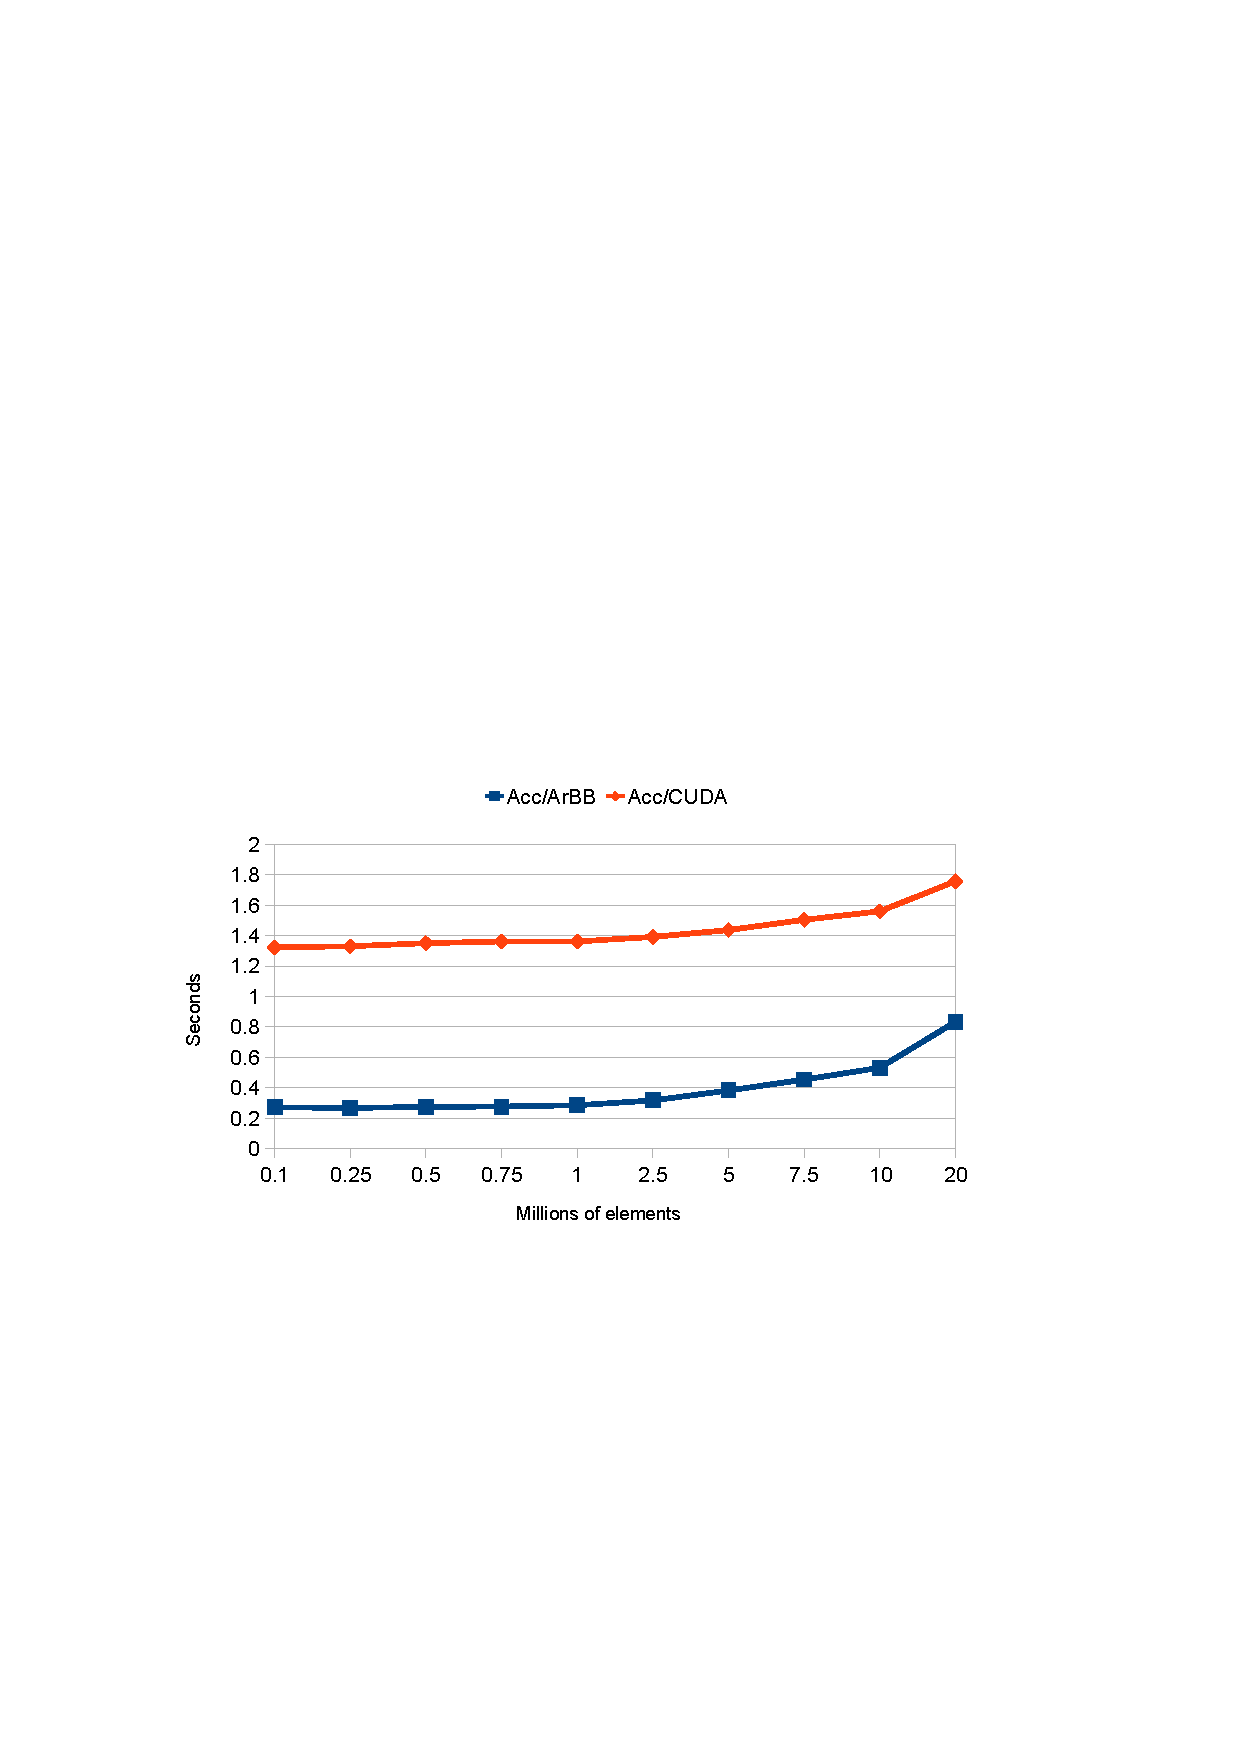
\includegraphics[width=3.5in]{./arbb/jit}    
  \end{center}
\vspace{-5mm}
  \caption{Running time experiments including JIT-time.} 
  \label{f:jit}
\end{figure}

\begin{figure}
  \begin{center}
   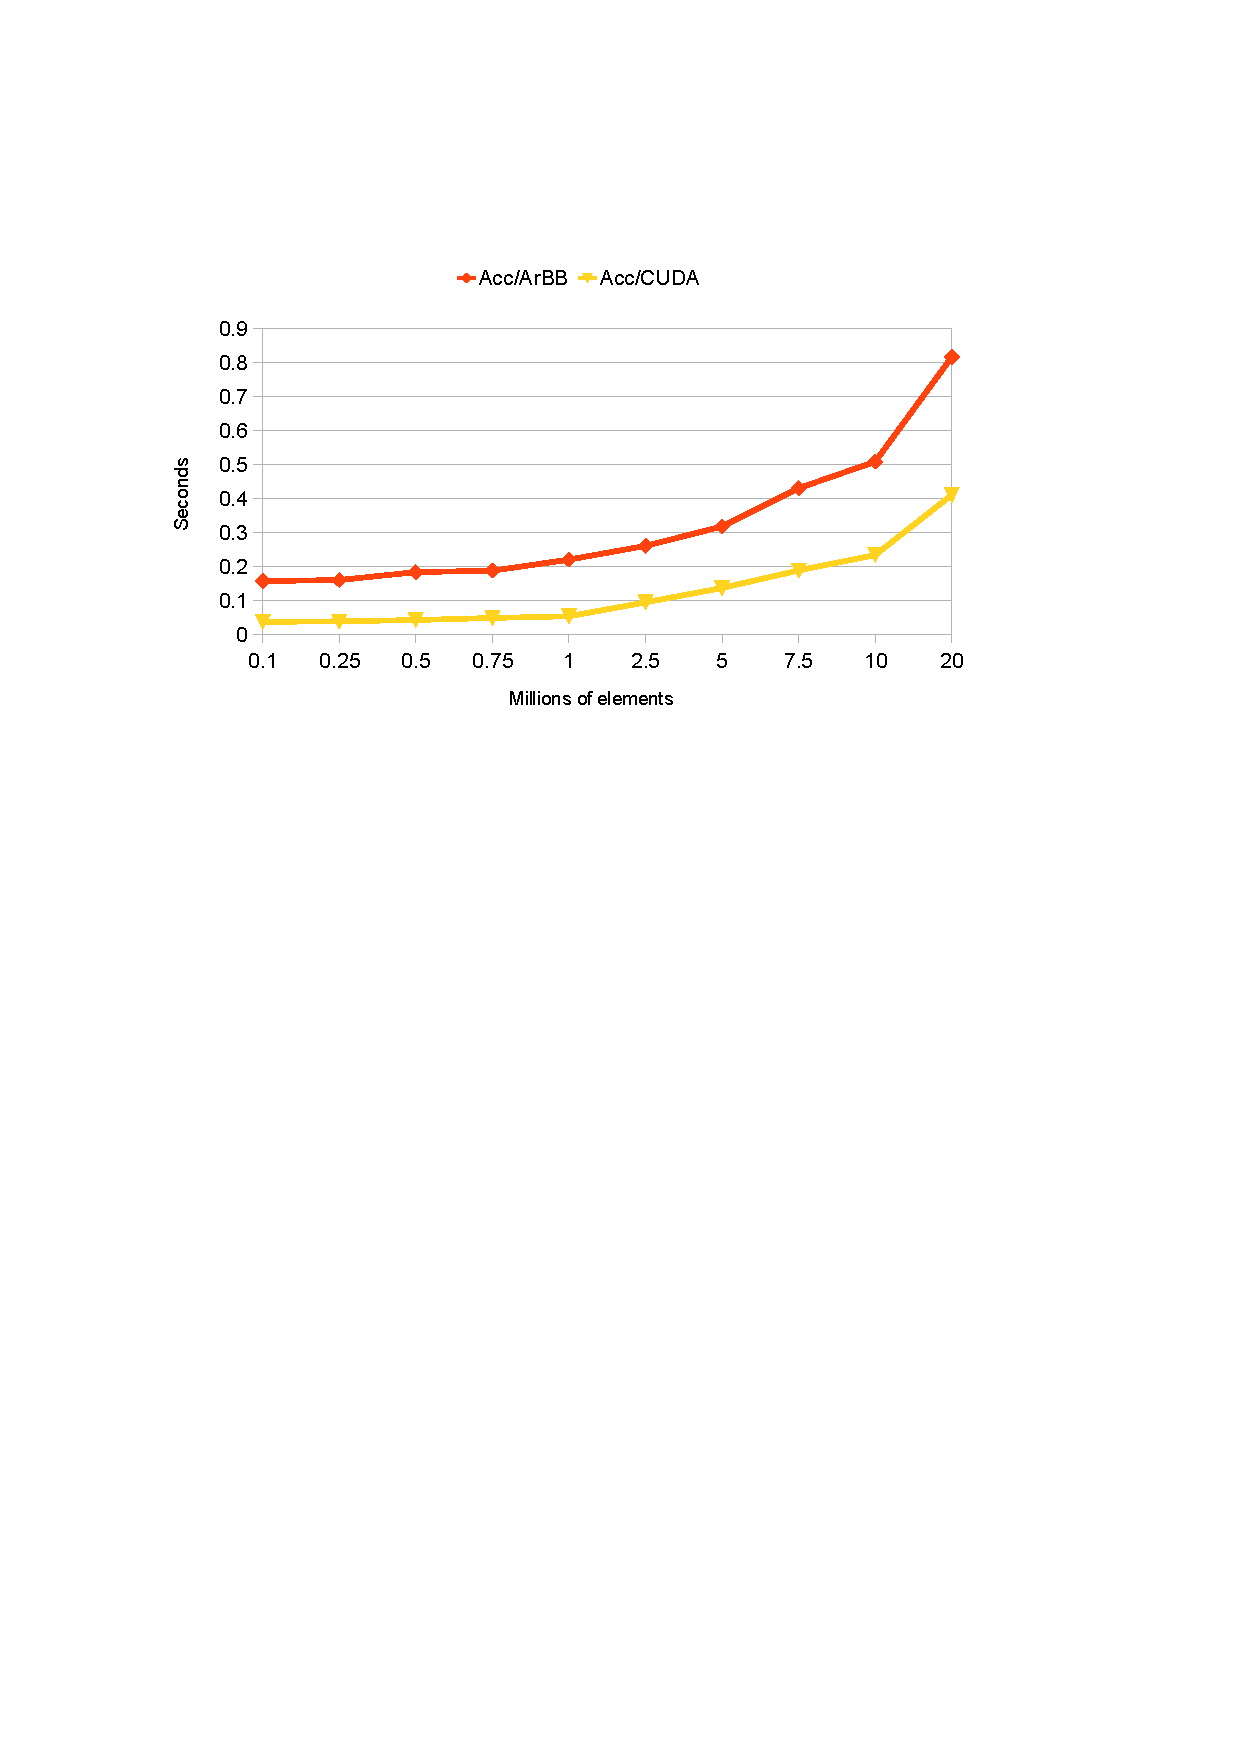
\includegraphics[width=3.5in]{./arbb/nojit}    
  \end{center}
\vspace{-5mm}
  \caption{Running time experiments JIT-time excluded.}
  \label{f:nojit}
\end{figure}


Figures~\ref{f:jit} and \ref{f:nojit} show preliminary results obtained on 
the Black-Scholes benchmark. The figures where obtained on a system with a 4-core 
Intel Core I7 975 machine with HyperThreading. The GPU used was a NVIDIA GTX480.

Figure~\ref{f:jit} shows running times obtained when JIT-time is included. 
% What this figure mainly tells us is that the JITing overhead 
JIT compilation time is much larger 
in the CUDA backend than the ArBB one.  Part of this difference 
can be attributed to the fact that 
the CUDA backend calls an external compiler (\cde{nvcc}), which takes its input in a file and runs in
a separate process.  ArBB, on the other hand, has a library interface to its  JIT-compiler. 
Figure~\ref{f:nojit} shows results obtained when pre-compiling the
CUDA functions eliminating JIT overhead.
In Accelerate, this happens automatically when the same kernel is
invoked repeatedly, because the Accelerate CUDA backed 
uses a caching scheme to avoid unnecessary JIT invocations.  (The
caching functionality has not yet been duplicated in the 
ArBB backend.)

These early results demonstrates the principle that even when a kernel
executes with higher throughput on a GPU, in a particular program it
is difficult to decide whether a computation is worth moving to a GPU,
incurring extra data-movement and possibly extra JIT compilation
\citearbb{wheres-the-data-paper}.  Specifically, we see that the
Accelerate Black-Scholes program from Figure~\ref{fig:blackscholes}
performs better on the CPU if it executes once (even on a large window
of data) whereas the GPU would yield better performance in a sustained
series of executions.
%
Because both CPU and GPU execution may be desirable---and the
selection may be dynamic---it is beneficial to have a single source code
that is portable across both.  
% Accelerate combined with \systemname{} makes this possible.


% ====================================================================================================
\subsection{Related Work}
% ====================================================================================================


OpenCL~\citearbb{opencl08} is a programming model very similar to CUDA but with the aspiration 
to offer both acceleration of computations on GPUs or to multicore CPUs. 
OpenCL JIT compiles the kernels for the particular hardware available and is
in that sense similar to ArBB.  
OpenCL programs are relatively low-level and require a large amount of
boilerplate to create and invoke.  In this sense they occupy a very
different niche than Accelerate.

Microsoft Accelerator~\citearbb{ACCELERATOR} is an embedded language with similar 
aspirations as ArBB, that is, to target a diverse range of architectures using the 
same source code. Accelerate can be used from the C\# language or the 
functional F\# language and targets GPUs or of CPUs and their
vector units.
% However, being part of the .Net framework implies limited accessibility 
%for platforms other than Microsoft Windows.  

\rn{What's the comparison with our stuff?}

%Most work on partitioning workloads between 
Many CPU and GPU comparisons, and some CPU/GPU workload partitioners \citearbb{merge}, rely on
redundant hand-written versions of all kernels
% \citearbb{cpu-gpu-partitioning} 
(though some systems like Qilin \citearbb{qilin} allow a single source code).
It is difficult in this kind of scenario
to make fair comparisons, controlling for the
amount of effort put into the respective implementations.
For example, comparing unoptimized serial CPU implementations vs. GPU
ones is not informative \citearbb{debunking-dubey}.
In \systemname{} controlling for effort
need happen only once---both CUDA and ArBB are
independently optimized by their respective teams of engineers---not for each benchmark.


% ====================================================================================================
% \section{Future work and Conclusions}
%\section{Future Work}
% ====================================================================================================

%\rn{need to be careful about being too repetitive...}
%The \accarbb{} backend is currently work-in-progress. The Accelerate
%functionality is not yet completely covered by the ArBB backend. Currently 
%the ArBB back-ed is operational for Accelerate programs using {\em Map}, 
%{\em ZipWith} and some simple instances of the Accelerate {\em Fold} operation.
%All of these also have the limitation that they only work for up to and 
%including 3-dimensional arrays using the ArBB backend while the Accelerate
%model allows the N-dimensional case. Allowing the N-dimensional case 
%in the ArBB backend for the supported operations range from a simple exercise 
%to more intricate problems needing some thought. For example, in the case 
%{\em Map} operations the needed transformation is simple (Accelerate Maps 
%over N-dimensional arrays is a per-element operation). One could flatten 
%the N-dimensional array to a 1-dimensional array (remembering its old shape) 
%perform the map and then transform the array back into N-dimensions. In 
%the case of {\em Fold} (reductions) the situation becomes more tricky. 
%transforming the arrays to arrays of lesser dimensionality then requires 
%a so-called segmented {\em Fold} operation. 

%The current \accarbb{} backend uses a hybrid of immediate-mode 
%and retained-mode programming styles. Moving more towards 
%retained-mode only may have performance benefits since it would give the 
%ArBB compiler larger programs to optimize. Exploring this aspect is left 
%as future work. 

% ====================================================================================================
\subsection{Discussion and Conclusions}
% ====================================================================================================

We have demonstrated that an EDSL such as Accelerate is sufficiently
platform-independent to break free of its original hardware target
(CUDA/GPU) and create efficient programs on other architectures.  This
gives us hope that \systemname{}/Accelerate programs will be
forward-portable to future parallel architectures and instruction
sets.

The EDSL approach changes the playing field for the designer
of compiler backends.  Rather than contending with full blown
languages and their complexities (e.g. pointers, aliasing,
inheritance, virtual functions, etc), compiler backends can focus on
simple value-oriented compute languages.

%% Achieving the ultimate goal of performance portability requires
%% progress on two research problems.  The first is EDSLs themselves and
%% their integration into host languages.  The second problem 

But the EDSL method solves only part of the performance-portability problem.
Simple as EDSL target languages may be, there remains a
substantial challenge in mapping them efficiently to the diversity
of parallel architectures available now and in the near future.
%especially without requiring a large amount of additional per-platform
%user annotations.
\textred{For example, the idiosyncrasies of memory bank access on
  NVIDIA GPUs must be taken into account to generate efficient
  implementations of the high-level collective operations that we have
  discussed.}

This is a compiler backend research challenge.
The {\em skeletons} method mentioned in
Section~\ref{sec:accelerate-arbb} is one approach to this problem, as
are the optimizations studied in the Copperhead \citearbb{copperhead} and
Obsidian \citearbb{JSLIC} projects.
%
On the other hand, systems that rely on advanced optimizations
typically suffer to some extent from performance-predictability
problems.  Thus achieving portable, predictable performance on a wide range
of architectures---even for the simplest target languages---will
be the subject of much future work.

%{
%\small
\bibliographystylearbb{alpha}
\bibliographyarbb{thesis}
%}


%\end{document}





% ---------------------------------------------------------------------------
% 
% ---------------------------------------------------------------------------
\cleardoublepage 

\section[\paperDTitle]{\paperD: \\ \paperDTitle}
\label{sec:paperD}
%\addcontentsline{toc}{chapter}{Expressive Array Constructs in an Embedded GPU Kernel Programming Language}

%\paperDTitle

\begin{center} 
Koen Claessen, Mary Sheeran, Bo Joel Svensson
\end{center}


%% bare_conf.tex
%% V1.3
%% 2007/01/11
%% by Michael Shell
%% See:
%% http://www.michaelshell.org/
%% for current contact information.
%%
%% This is a skeleton file demonstrating the use of IEEEtran.cls
%% (requires IEEEtran.cls version 1.7 or later) with an IEEE conference paper.
%%
%% Support sites:
%% http://www.michaelshell.org/tex/ieeetran/
%% http://www.ctan.org/tex-archive/macros/latex/contrib/IEEEtran/
%% and
%% http://www.ieee.org/

%\documentclass[conference]{IEEEtran}

%\usepackage{graphicx, color, code}
%\usepackage[cmex10]{amsmath}
%\usepackage{url}
% \usepackage{bookman}  %% bold teletype fonts, but don't know how to prevent it from changing the whole document

% Haven't figured out how to get this to work properly:
%\usepackage[\texttt{cmbtt}]{bold-extra}
% \usepackage{bold-extra} 

%\usepackage{courier}
%\usepackage{fancyvrb}

% correct bad hyphenation here
%\hyphenation{op-tical net-works semi-conduc-tor}


%====================================================================================================
%% FIRST, MISC USEFUL DEFINITIONS
%====================================================================================================

\definecolor{darkgreen}{rgb}{0, 0.5, 0}
\definecolor{darkblue}{rgb}{0,0,0.5}
\definecolor{mygrey}{rgb}{0.7,0.7,0.7}
\newcommand{\textblue}[1]{\textcolor{blue}{#1}}

\newcommand{\cde}[1]{{\footnotesize \tt #1}}

% \newcommand{\kw}[1]{{\bf{#1}}}
\newcommand{\kw}[1]{{\textbf{#1}}}

\newcommand{\comm}[1]{{\em \textcolor{darkgreen}{#1}}}  %% Code comments

\newcommand{\note}[1]{\begin{itemize}\item \textcolor{blue}{#1} \end{itemize}}

%% \newenvironment{mycode}
%% {% This is the begin code
%%   \begin{Verbatim}[commandchars=\\\{\}]}%
%%   %\footnotesize
%%   %\noindent
%%   %\begin{code}\noindent\vspace{-1mm}}
%% %  \begin{code}\noindent}
%% {% This is the end code
%%   \end{Verbatim}
%%   %\end{code} 
%% }

%% \newenvironment{inlinecode}
%% {
%%   \begin{center}
%%   \begin{minipage}{4in}
%%   \begin{mycode}
%% } 
%% {
%%   \end{mycode}
%%   \end{minipage}
%%   \end{center}
%%   \vspace{-1.5ex}
%% }

%% ============================================================
%% USE TO DISABLE COMMENTS:
 \def\noeditingmarks{}
%% ============================================================
\ifx\noeditingmarks\undefined
   \newcommand{\textred}[1]{\textcolor{red}{#1}}
   \newcommand{\pgwrapper}[2]{\textred{#1: #2}}
%   \newcommand{\pgwrapper}[2]{}
   \newcommand{\rnote}[1]{\begin{itemize}\item{\textcolor{blue}{#1}}\end{itemize}}
   \newcommand{\new}[1]{\textcolor{blue}{#1}}
   \newcommand{\const}[1]{\textred{#1}}

%% RRN: Dim the background for Ryan's eyes:
%%   What I need here is a way to do it based on user or host name...
% \pagecolor{mygrey}

\else
   \newcommand{\textred}[1]{#1}
   \newcommand{\pgwrapper}[2]{}
   \newcommand{\rnote}[1]{}
   \newcommand{\new}[1]{#1}
   \newcommand{\const}[1]{#1}
\fi

\newcommand{\js}[1]{\pgwrapper{BJS}{#1}}
\newcommand{\rn}[1]{\pgwrapper{RRN}{#1}}


%% Can we call our ``things'' 
%% ArBB/Haskell for the bindings part ? 
%% Accelerate/ArBB for the Accelerate backend ?
%% This would work with the convention we adopted for 
%%      ArBB/C++  
\newcommand{\systemname}[0]{{Harbb}}
%\newcommand{\systemname}[0]{\textred{HArBB}}

%% This could in theory be separate from the project name..
\newcommand{\accarbb}[0]{\systemname{}}

%% NOTE: THIS SHOULD BE THE SAME AS SYSTEMNAME:
\newcommand{\arbbvmH}[0]{ArBB/Haskell}


%====================================================================================================
% END DEFINITIONS
%====================================================================================================




%\begin{document}
% \title{Painless Portable Vector Parallelism\\ with Haskell and Intel ArBB}
%\title{Programming Future Parallel Architectures\\ with Haskell and Intel ArBB}
% \title{Embedded Domain-Specific Languages Pave the Way for New Parallel Architectures}

%\author{\IEEEauthorblockN{Bo Joel Svensson}
%\IEEEauthorblockA{Dept. of Computer Science and Engineering\\
%Chalmers University of Technology\\
%Gothenburg, Sweden\\
%Email: joels@chalmers.se}
%\and
%\IEEEauthorblockN{Ryan Newton}
%\IEEEauthorblockA{Intel Corporation\\
%Hudson, MA\\
%Email: rrnewton@gmail.com
%}}
% Email: ryan.r.newton@intel.com

%\maketitle

%\begin{abstract}
%
\subsection*{Abstract}
New parallel architectures, such 
\new{as Cell, Intel MIC, GPUs, and tiled architectures, enable} high
performance but are often hard to program.
What is needed is a bridge between high-level programming models 
where programmers are most productive and modern parallel architectures. 
We propose that that bridge is Embedded Domain Specific Languages (EDSLs). 

\new{One attractive target for EDSLs is}
Intel ArBB, a virtual machine for parallel, vectorized computations.
% that serves as a compilation target for EDSLs.
We propose to wed ArBB with the functional programming language
Haskell, {using an EDSL} that generates code for the ArBB VM.  This Haskell integration provides 
% a determinism guarantee 
added safety guarantees compared to other ArBB interfaces.
%
Further, our prototype, \systemname{}, is one of the first EDSL implementations with
optimized backends for multiple parallel architectures (CPU, \new{NVIDIA GPU}, and
others), allowing portability of source code over devices
and their accelerators.


%\end{abstract}
%\IEEEpeerreviewmaketitle




% ====================================================================================================
\subsection{Introduction}
% ====================================================================================================

Are radical new parallel architectures market-feasible if they require
significant changes for programmers?  The jury is out.  In recent
years we have seen difficult-to-program chips suffer 
% \citearbb{cell} 
(e.g. Cell)
and
GPU vendors strive to enable more traditional programming features
\citearbb{fermi} (e.g. C++).  There is an increasing
tension between ease of programming and efficiency.

The tension  shows  across diverse chip markets.  For example,
small embedded devices are most power efficient if their processors and operating systems
omit programming features such as virtual memory and threads \citearbb{tinyos}.  
At the other end of the power spectrum, GPU's
graphics performance may suffer due to inclusion of hardware to ease
GPGPU programming.  In short, there is an opportunity cost to
including extra hardware for programmability.

In this paper, we argue 
that a specific technique holds the greatest promise of solving the programmability dilemma.
%
Domain-specific languages, {\em embedded} within general purpose
languages (EDSLs) 
 enable familiar programming models 
{\em and} flexible
mapping onto new hardware.  The key to having this cake and eating it
too is {\em metaprogramming}.  Familiar programming features are
present, but are eliminated at an intermediate (metaprogram evaluation)
phase and therefore do not reach the parallel hardware itself.


% We present our ongoing work on a
In pursuit of this vision, we offer a
% 
 new EDSL implementation, called \accarbb{}, that combines
existing systems, Accelerate \citearbb{ACCELERATEDAMP11} and ArBB \citearbb{ArBB}, to produce a unified
high-level programming environment equally suited to multicore,
vectorized CPUs, as to GPUs and other accelerators (such as Intel MIC chips \citearbb{larrabee}).
%
\if{0}
ArBB is based on the RapidMind \citearbb{RapidMind} system which was an embedded 
DSL targeting multicore CPUs as well as GPUs. ArBB does not \new{yet} include a GPU 
backend like RapidMind, targeting multicore CPUs and their vector 
units. 
\fi{}
\systemname{} is a single EDSL implementation 
with independently optimized backends \new{by different teams; 
namely, the ArBB backend for CPU/MIC, and a CUDA backend for NVIDIA GPU.}
This makes
\systemname{} an appealing platform for fair CPU/GPU comparisons, 
as well as a compelling programming model for single-source portable performance across a range of
parallel architectures, \new{present and future}.
%%To our knowledge, \systemname{} is the first EDSL implementation with
%%independently optimized backends for CPUs and GPUs.  This makes
%%\systemname{} an appealing platform for fair CPU/GPU comparisons, 
%%as well as a compelling programming
%%model for single-source portable performance across a range of
%%parallel architectures.


% ====================================================================================================
\subsection{Embedded Domain-Specific Languages}
% ====================================================================================================


Domain-specific languages---from Makefiles and \LaTeX{} to
Matlab---are almost too ubiquitous to notice.  Most relevant to our
purposes, domain-specific languages (DSLs) that target a narrow domain and expose communication
patterns to the compiler 
 have achieved performance-portability across a wide range of parallel
architectures.  
StreamIt\citearbb{streamit} is a good example.
% (for example, StreamIt\citearbb{streamit})
% The high-water mark in this area is perhaps  StreamIt\citearbb{streamit}.
% 

% It has been noted \citearbb{not-sure} that 
% Yet the few DSLs that gain popularity lose simplicity\citearbb{not-sure}.  
% Yet popular DSLs rarely remain simple \citearbb{not-sure}.  
DSLs may start out simple and focused, but if they gain popularity
they quickly grow in complexity to rival full-blown languages.
Feature creep
can make DSL implementations complex and expensive to maintain.
Further, non-standard DSL syntax and features present a learning curve for users.  In the
last ten years an attractive solution to this dilemma has emerged: {\em
  embed} each DSL into a general-purpose host language that can provide
common functionality with familiar syntax and semantics.
% in place of the DSL.

When embedding, host language programs {generate} DSL programs;
% Embedding means that the host language is used to generate DSL programs; 
the {\em deeper} the embedding, the more integrated the
DSL into the syntax and type-system of the host language.
%
% Typically, %% pruning weasel words
A key host-language feature for embedding is that
language constructs can be overloaded to operate over {\em abstract
  syntax trees} (ASTs)\footnote{This ad-hoc polymorphism is accomplished,
for example, through operator-overloading in C++ or type classes in
Haskell.}.  For example, the following simple function operates on scalars:


\vspace{1mm}
\begin{Verbatim}[commandchars=\\\{\}]
  float f(float x) \{ return (2*x - 1); \}
\end{Verbatim}
\noindent
But simply by changing the types, \cde{f} might be lifted to operate on {\em
  expressions} (which, when evaluated, will yield \cde{floats}):

\vspace{1mm}
\begin{Verbatim}[commandchars=\\\{\}]
  \kw{exp<float>} f(\kw{exp<float>} x) \{
    return (2*x - 1);
  \}
\end{Verbatim}

A common arrangement is for the host language program to execute at
runtime but to generate ASTs that are executed by a just-in-time
(DSL) compiler.  This use of metaprogramming (program generation)
differs from the more common usage of preprocessors and 
% Lisp/Scheme macros \citearbb{scheme-macros}
macros, which typically add extra
phases of computation {\em before}  compile time---increasing
the number of compile-time rather than runtime phases.

% EDSLs typically add additional runtime phases.  That is, the host language program 
% executes at runtime but uses a JIT to process generated ASTs.
%% which are
%% usually used to perform computation {\em earlier} than the usual
%% compile time, embedded DSLs (EDSLs) typically defer computation 


One reason that EDSLs are good for productivity is that the programmer
gains the software engineering benefits of the host language
(object-orientation, higher-order-functions, modules, etc), while not
paying the cost at runtime for additional layers of abstraction or
indirection.  Indeed, the embedded languages for 
performance-oriented EDSLs are often simple, first-order
languages without pointers \citearbb{wavescript, ACCELERATEDAMP11}.

% , paul-lius-thingy

% regiment,
As a research area, EDSLs and two-stage DSLs have been actively pursued for at least a
decade \citearbb{VERTIGO, wavescript} but are gaining steam
recently 
%\citearbb{sejits, stanford-ppl} 
\citearbb{copperhead, stanford-ppl} 
and are beginning to appear in
commercial products \citearbb{ArBB}.
%
Further, EDSL techniques have spread beyond their origin in 
 the programming languages community.
% 
For example, both Stanford's Parallel Programming Laboratory (PPL) and
the Berkeley Parlab are creating EDSLs as their flagship parallel
programming solutions for domains such as machine learning and
rendering \citearbb{stanford-ppl}.
  Moreover, EDSLs need not be hosted by esoteric research languages---Intel's
 ArBB embeds an array language in C++ and Berkeley's
Copperhead \citearbb{copperhead} generates CUDA from simple Python code.

%\rnote{Is there a good motivating example program?  What are some of
%  the Metaocaml motivating examples?}

{For the remainder of this paper we will focus our discussion
  on the Intel ArBB VM, a virtual machine for just-in-time
  generation of vector codes, \new{which implements a restricted} domain-specific
  language of array computations.  In this paper we introduce
  {\em High-level ArBB}, 
  (\systemname{}), an EDSL that internally uses the ArBB
  VM.  \new{While Intel's ArBB package already includes an EDSL targeting the VM (for C++)},
\systemname{} \new{offers additional advantages, including}
  more succinct programs and additionally safety
  guarantees---namely, complete deterministic-by-construction parallel
  programs (across both host and VM languages).}


% ====================================================================================================
% \section{Accelerate and ArBB}
%\section{\accarbb{}:  ArBB and Accelerate}
\subsection{\accarbb{} $=$ ArBB $+$ Accelerate}
\label{sec:accelerate-arbb}
% ====================================================================================================

Our first \systemname{} prototype adapts an existing EDSL called {\em
  Accelerate} (Data.Array.Accelerate).  Accelerate targets high-level
data-parallel programming in Haskell.
Previous work on Accelerate has focused on developing a CUDA-backend
for GPU programming.  In this paper we describe our effort to retarget
Accelerate to ArBB.  

With respect to determinism guarantees, the existing Intel ArBB product
represents an integration of the safe (ArBB VM) with the unsafe (C++).
In the Haskell context, because purely functional computations are
guaranteed deterministic (even when executed in parallel), and because
ArBB computations invoked by Haskell functions are themselves free of
side-effects, \systemname{} achieves a
guarantee of determinism for complete programs that combine both
Haskell computation and ArBB VM computation.
% which offers portability.
% (The 'H' in \systemname{} therefore stands for Haskell as well as ``High-level''.)


%% {\em Accelerate} (Data.Array.Accelerate) is an existing EDSL for 
%% high-level data-parallel programming in Haskell~\citearbb{Accelerate}. 
The Accelerate programming model consists of collective 
operations that can be performed over arrays, together with a simple 
language of scalar expressions\new{---in the current release, the Haskell type system enforces that parallelism not be nested.}
\if{0}
The Haskell type 
system is used to enforce that no nested data-parallelism can be expressed 
\new{(in the current release, this may be relaxed in the future).}
\fi{}
Accelerate's collective operations include {\em Map} (akin to parallel
for loops) {\em ZipWith} (a generalization of elementwise vector addition) and 
{\em Fold} (sum generalized)---familiar operations for programmers versed in the functional paradigm.
All of these collective operations are easily parallelizable. 
% In the case of {\em Map} and {\em ZipWith} the potential for parallelism is abundant.  

%% dotProd :: Vector Float -> 
%%            Vector Float -> 
%%            Acc (Scalar Float) 
\begin{Verbatim}[commandchars=\\\{\}]
dotProd (xs :: Vector Float) 
        (ys :: Vector Float) = 
  \kw{let} xs\_ = use xs 
      ys\_ = use ys 
  \kw{in}  fold (+) 0 (zipWith (*) xs\_ ys\_) 
\end{Verbatim}

The Accelerate code listing above specifies a function that takes two 1-dimensional 
arrays as inputs (of type \cde{Vector Float}, e.g. a vector of floats). The result of the function is a single
scalar. 
% (\cde{Scalar Float})
The \cde{use} function is applied to an array to convert it 
for use in the collective operations provided by Accelerate;
\cde{use} 
% is actually a function with type \cde{Vector a -> Acc (Vector a)} and 
may result in
copying the array to, for example, the GPU in the case of Accelerate's 
CUDA backend.  

After applying \cde{use} to bring in input data, the programmer then
constructs a data-parallel program from collective operations.
Above, \cde{fold} is a function that takes three arguments, 
here those arguments are \cde{(+)},  $0$ and \cde{zipWith (*) xs\_ ys\_}. 
\cde{zipWith}, in turn, is a function taking three arguments, \cde{(*)}, 
\cde{xs\_} and \cde{ys\_}. The \cde{zipWith} operation here applies pairwise 
multiplication to the two arrays and the \cde{fold} sums up all the elements 
into a single scalar. 

%\rn{Following para slightly redundant but ok...}
%Accelerate makes GPU programming accessible to the functional programmer 
%by offering a familiar set of operations. This set of operations also have 
%the beneficial property that they have inherent parallelism and are 
%easily implementable on the GPU. 

Accelerate's CUDA backend implements collective operations using
a hand-tuned ``skeleton'' for each operation (and possibly for
different hardware versions). The kernel---for example, the function
to mapped over the dataset---is 
instantiated into the body of the skeleton code. The resulting 
program is compiled using the NVIDIA CUDA compiler and dynamically linked 
into the running Haskell program.

%\subsection{Intel Array Building Blocks (ArBB)}
\subsection{Intel Array Building Blocks (ArBB)}
\label{sec:arbb}

%ArBB is embedded in the C++ programming language but it also exposes a 
%very low level API that is purely C. 
%{\em ArBB} (Array Building Blocks) is also an embedded DSL. 
The operations exposed by ArBB are similar to those of Accelerate. 
In ArBB, parallel computations are expressed using a set of built-in 
primitives. All vectorization and threading is managed internally by 
ArBB. The programmer uses collective operations with a clear semantics 
such as \cde {add\_reduce} that computes the sum of the elements in a given 
array. ArBB also has language constructions for control flow, conditionals
and loops. These operations have their usual sequential semantics and are not 
parallelized by the system, rather, only specific collective operations are executed
in parallel. 

Today's existing ArBB product is embedded in C++ and provides special
types for scalars and arrays (e.g. \cde{dense<f32>} rather than \cde{vector<float>}).
Using ArBB/C++ to express the dot product computation can be done 
as follows:

%\vspace{2mm}
\begin{Verbatim}[commandchars=\\\{\}]
\kw{void} dot\_product(\kw{const} dense<f32>& a, 
                 \kw{const} dense<f32>& b,
                 f32& c) 
{ 
  c = add\_reduce(a * b);
}
\end{Verbatim} 


% The above program takes two arrays of type \cde{dense<f32>} as input. 
% \cde{dense<f32>} specifies a 1-dimensional array of 32-bit floating
% point values. The result is a single 32-bit float.  

Note that arithmetic operators such as (*) are overloaded 
for to operate on arrays as well as scalars (e.g. \cde{a * b} above).
Thus, the above C++ function multiplies two arrays before summing them with \cde {add\_reduce}:

The code listing below is indicative to the amount of glue code needed to invoke an 
ArBB computation\footnote{In OpenCL and CUDA the glue code situation is even worse}. It shows how the dot product code is launched using {\tt call} and 
how data is bound, {\tt bind}, for use in ArBB. 

\vspace{2mm}
\begin{Verbatim}[commandchars=\\\{\}]
\kw{int} main() 
\{ 
  double a[SIZE];
  double b[SIZE];

  for ( \kw{int} i = 0; i < SIZE; ++i) \{ 
    a[i] = ...; b[i] = ...;
  \}
  dense<f32> va, vb;
  f32 vc;
  bind(va, a, SIZE); 
  bind(vb, b, SIZE); 
  call(dot\_product)(va, vb, &vc); 
  ...
\}
\end{Verbatim}


%\rnote{SPECIFICALLY ADDRESS THE FUNCTIONALITY GAP?  E.G general
%  reduce.  Any other examples?}

The model provided by Accelerate is slightly richer than that of ArBB.
Even the two very simple \cde {dot\_product} examples above manage to illustrate 
this. In Accelerate there is a more general reduction primitive called \cde {fold} 
where in ArBB there are specific reductions, \cde {add\_reduce}, \cde {mul\_reduce} 
and so on. Not visible in these small examples is another difference, Accelerate 
operations are generalized to arbitrary dimensions while ArBB operations are 
limited to 1, 2, and 3 dimensions (and 0, i.e. scalar). These differences aside,
the ArBB and Accelerate programming models are very similar.


% ====================================================================================================
\subsection{Implementation of \systemname{}} 
% ====================================================================================================


%\rnote{Sadly the Haskell details don't buy us much here... what are
%  the {\em conceptual} problems solved in mapping the Accelerate
%  abstraction to the ArBB one?  The data models are similar, but
%  there are always mismatches -- dimensionality support, missing
%  reduction.}

%\rnote{What is the technique that you are using to address these sorts
%  of problems?  Is there anything to say about it?}

\begin{figure}
  \begin{center}
   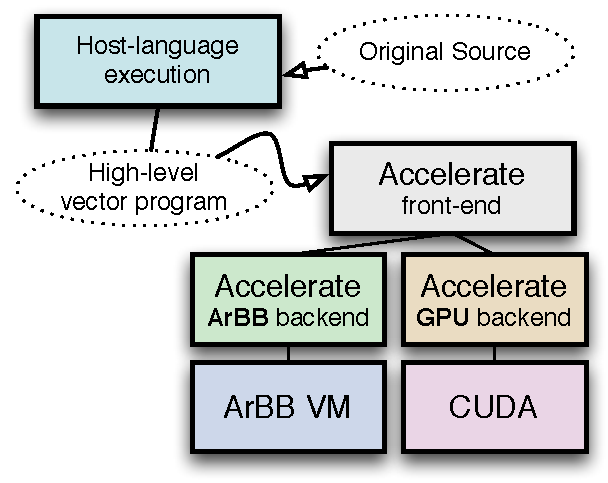
\includegraphics[width=2.0in]{./arbb/figure_architecture}    
  \end{center}
\vspace{-5mm}
  \caption{Architecture of the \systemname{} system.  \rn{(ROUGH.)}}
  \label{f:architecture}
\end{figure}


Using Accelerate and ArBB together, we propose a layered architecture
for \systemname{},
% Our goal is to make the benefits of ArBB available to the Haskell programmer. 
% \js{(Or is our goal to give an even better ``front-end'' to ArBB compared to C++)}
% We propose that this is best accomplished using a layered approach, as
pictured in Figure~\ref{f:architecture}. 
The host language execution (via Haskell in this case) executes the
programmer's source code, generating a vector program in the
restricted language of the Accelerate front-end.
Then either Accelerate backend---ArBB or CUDA---may be used.
The 
bottom layer of the ArBB backend consists of a direct mapping of the ArBB virtual machine
API (VMAPI) into Haskell including one-to-one bindings for each C 
function. 
To [partially] automate the creation of these bindings we used the C2HS system \citearbb{C2HS}. The 
\arbbvmH{} bindings are very low-level.
%and make little use of the high-level programming methods that
% Haskell programmers want. 
The idea 
is that the \arbbvmH{} bindings should be used to implement
backends for higher-level data-parallel EDSLs.

%% To illustrate our position we 
%% have started working on a backend to the successful DSL Accelerate 
%% (Data.Array.Accelerate) using our \arbbvmH{} bindings. 

To address the functionality mismatch between Accelerate and ArBB,
when possible we reencode the users Accelerate program using existing
ArBB mechanisms.  Our prototype does not support 100\% of Accelerate's
compute model (for example, only supporting  up to three-dimensional
arrays), but the remaining functionality can be mapped onto ArBB in
time using known methods---for example, our compiler could map higher
dimensional arrays onto a specific lower-dimensional data-layout.

%% The programming models supported by ArBB and Accelerate are very similar. 
%% Both obtain their parallelism by exposing collective operations 
%% such as {\em Map}, {\em Reduce}, {\em ZipWith} and {\em Scan} (all prefixes operations). However, 
%% the functionality match is not 100\%. For example, Accelerate supports {\em Map} operations 
%% over N-dimensional Arrays while ArBB supports them only up to 3-dimensions. 
%% Similar inconsistencies apply to the other operations as well. \textred{The current
%% ArBB backend simply disallows Accelerate programs using too high dimensionality
%% of the arrays.} \rn{Sure, we want to say that we're not done closing
%%   this gap (for
%%   accuracy) but more importantly we want to identify whether
%%   techniques exist to close the gap.  Presumably, yes?  We can
%%   ourselves collapse the dimensionality of arrays before giving them
%%   to ArBB?  Are there any operations that would defeat that technique?}
%

One example of a functionality discrepancy bridged by our
implementation is reductions.  As mentioned in \ref{sec:arbb},
Accelerate allows the programmer to reduce using an arbitrary
associative function, but ArBB has only built-in reductions with fixed
operations (add, multiply, xor, etc). We plan to provide general reductions in
the ArBB backend by a two-fold strategy:

\begin{enumerate}
\item Attempt to map an Accelerate reduction directly onto an ArBB
  primitive such as \cde{add\_reduce}.
\item Apply a general reduction technique based on $log(N)$ map
  operations over successively halving array sizes.  Essentially, cut
  the array in half, combine the halves, repeat. In ~\citearbb{reduction}
  this approach is explained in the context of CUDA. 
\end{enumerate}

%% \rn{Is the technique worthy of
%%   description?  Can we just cite the CUDA documentation or something
%%   since it's common?} 

In our current experiments, approach (2) is significantly slower.
Therefore, the ideal would be that ArBB exposed general reduction
directly in its programming model.  We expect this functionality to be
added in future releases.  In the meantime we plan to explore a
technique that would allow us to maximize the number of situations in
which (1) above applies.  Namely, a reduce operation can often be {\em
  factored} into a map followed by a reduce.  For example, a reduction
that multiplies each input number by a coefficient and sums the
results can be split into a map phase for the multiplication followed
by the built-in \cde {add\_reduce} operator.

%% Currently, our reduction implementations in ArBB 
%% are many times 
%% slower (\textasciitilde 20x) than their built-in counterparts. 
%% % To ameliorate this present performance problem we attempt to map
%% % programmers 
%% Our present workaround for this performance problem is to let 
%% \accarbb{} inspect the reduction function and switch to efficient 
%% built in  ArBB reduction where possible.  
%% \rn{Future work may be to decompose reductions into map+reduce so as
%%   to allow the reduce to become a builtin.}


Another choice faced by our implementation is the granularity at which the
ArBB JIT is invoked.  Specifically, should each collective operation result in its
own call to the ArBB JIT (in ArBB terminology, {\em
  immediate-mode}, akin to the pre-OpenGL 3.0 immediate mode), or
should multiple collective operations be placed together
inside an ArBB function and passed to the JIT?
We will call the latter approach {\em retained-mode}.

%% In immediate-mode the 
%% operations called from the ArBB API are executed
%% synchronously---before each API call returns. In retained-mode, ArBB
%% collects calls and, only when results are requested, the 
%% entire computation is optimized 
%% and executed. 

Retained-mode generally offers performance benefits; a bigger 
chunk is given to the JIT compiler, enabling cross-optimization
between collective operations. 
Our prototype Accelerate backend uses 
ArBB in  
a combination of immediate- and retained-mode. The main collective 
operations are compiled using the retained-mode. For example, in the case 
of a \cde{map f}  operation first the function to be mapped is created and 
compiled using retained-mode then a small {\em mapper} function is 
also created and compiled using retained-mode. 
%% The mapper function is 
%% of course very small and therefore does not give much to the JIT compiler 
%% to work on optimization-wise. 
Between the collective operations the backend
needs to perform data management and copying, which 
are performed in immediate-mode. It is our belief that 
\systemname{} would benefit from using retained-mode exclusively 
but we leave that as future work. 





% ====================================================================================================
\subsection{Preliminary Results}
% ====================================================================================================

%\rnote{One tiny benchmark if we can manage it.}

%\rnote{Ideally: Something like blackscholes running Arbb/C++,
%  \systemname{}, CPU+GPU, possibly compared to other blackscholes
%  implementations -- say Cilk on CPU and hand-coded CUDA (I can
%  provide the former I think).  Perhaps serial, non-vectorized CPU for
%  comparison.}

%\rnote{Point 1 -- High level thing is within X\% of low level thing.
%  The usual.  But we also want to say that \systemname{} is no worse
%  than ArBB/C++ -- the metalanguage doesn't matter, be it Haskell,
%  Python, or C++.}

%\rnote{Point 2 -- It's important to do a good job on the CPU side.
%  Even if you don't beat GPU there's a big difference between
%  vectorizing/not-vectorizing (and using multicore of coarse).  Can't
%  be ignored.}

%\rnote{Bonus points -- if we could show how bad ``naive'' ports are that
%  would be nice.  How well does your C CPU code run on GPU unmodified
%  (or minimally ported)?}



%\rnote{CPU/GPU systems that do a good job of both.  Perhaps quickly
%  dismiss those that make no effort on the CPU side.}

Black-Scholes option pricing is a finance-related benchmark that has been used in similar
DSLs targeting GPUs \citearbb{ACCELERATEDAMP11, NIKOLA}. Since we are re-using the 
Accelerate front-end, we can directly use the Black-Scholes benchmark that 
is shipped with that system.  Figure \ref{fig:blackscholes} shows the
complete code listing for an Accelerate Black-Scholes function which
can be executed on GPUs or any processor targeted by ArBB.

% blackscholes :: Vector (Float, Float, Float) 
%
%                -> Acc (Vector (Float, Float))
%\fbox{

%       r     = \textit{constant} riskfree
%       v     = \textit{constant} volatility

\begin{figure}
\begin{footnotesize}
\begin{Verbatim}[frame=single, commandchars=\\\{\}]
blackscholes (xs :: Vector (Float,Float,Float)) = 
  map kernel (\textit{use} xs)

kernel x =
  \kw{let} (price, strike, years) = \textit{unlift} x
      r     = 0.02 \textsf{\textit{-- riskfree constant}}
      v     = 0.30 \textsf{\textit{-- volatility constant}}
      sqrtT = sqrt years
      d1    = (log (price / strike) + 
                   (r + 0.5 * v * v) * years) / 
              (v * sqrtT)
      d2    = d1 - v * sqrtT
      cnd d = d >* 0 ? (1.0 - cndfn d, cndfn d)
      cndD1 = cnd d1
      cndD2 = cnd d2
      expRT = exp (-r * years)
  \kw{in} \textit{lift} ( price * cndD1 - 
            strike * expRT * cndD2
          , strike * expRT * (1.0 - cndD2) - 
            price * (1.0 - cndD1))

cndfn d =
  \kw{let} poly  = horner coeff
      coeff = [0, 0.31, -0.35, 1.78, -1.82, 1.33]
      rsqrt = 0.39894228040143267793994
      k     = 1.0 / (1.0 + 0.2316419 * abs d)
  \kw{in} rsqrt * exp (-0.5*d*d) * poly k

horner coeff x = 
  \kw{let} madd a b = b*x + a
  \kw{in}  foldr1 madd coeff
\end{Verbatim}
\end{footnotesize}
\caption{Complete code listing for a Black-Scholes function expressed
  in Haskell syntax using the Accelerate and \systemname{} libraries.
  Invocations of the functions \cde{use}, \cde{lift} and \cde{unlift}
%  and \cde{constant} 
represent additional boilerplate added for
  conversion in and out of Accelerate types.  Specifically, \cde{lift} and
  \cde{unlift} convert tuples and handle the fact that Accelerate
  arrays of tuples are really implemented as tuples of arrays.
  Otherwise, the program is identical to a plain Haskell
  implementation.}
\label{fig:blackscholes}
\end{figure}


%% \end{code}
%%  %605993438
%% % horner :: Num a => [a] -> a -> a
%% \begin{code}
%% \footnotesize



The kernel of this algorithm performs arithmetic on triples of
floating point numbers, creating pairs of floats as results. The problem 
is embarrassingly parallel, consisting of independent computations
for every element of an array (a map).

\begin{figure}
  \begin{center}
   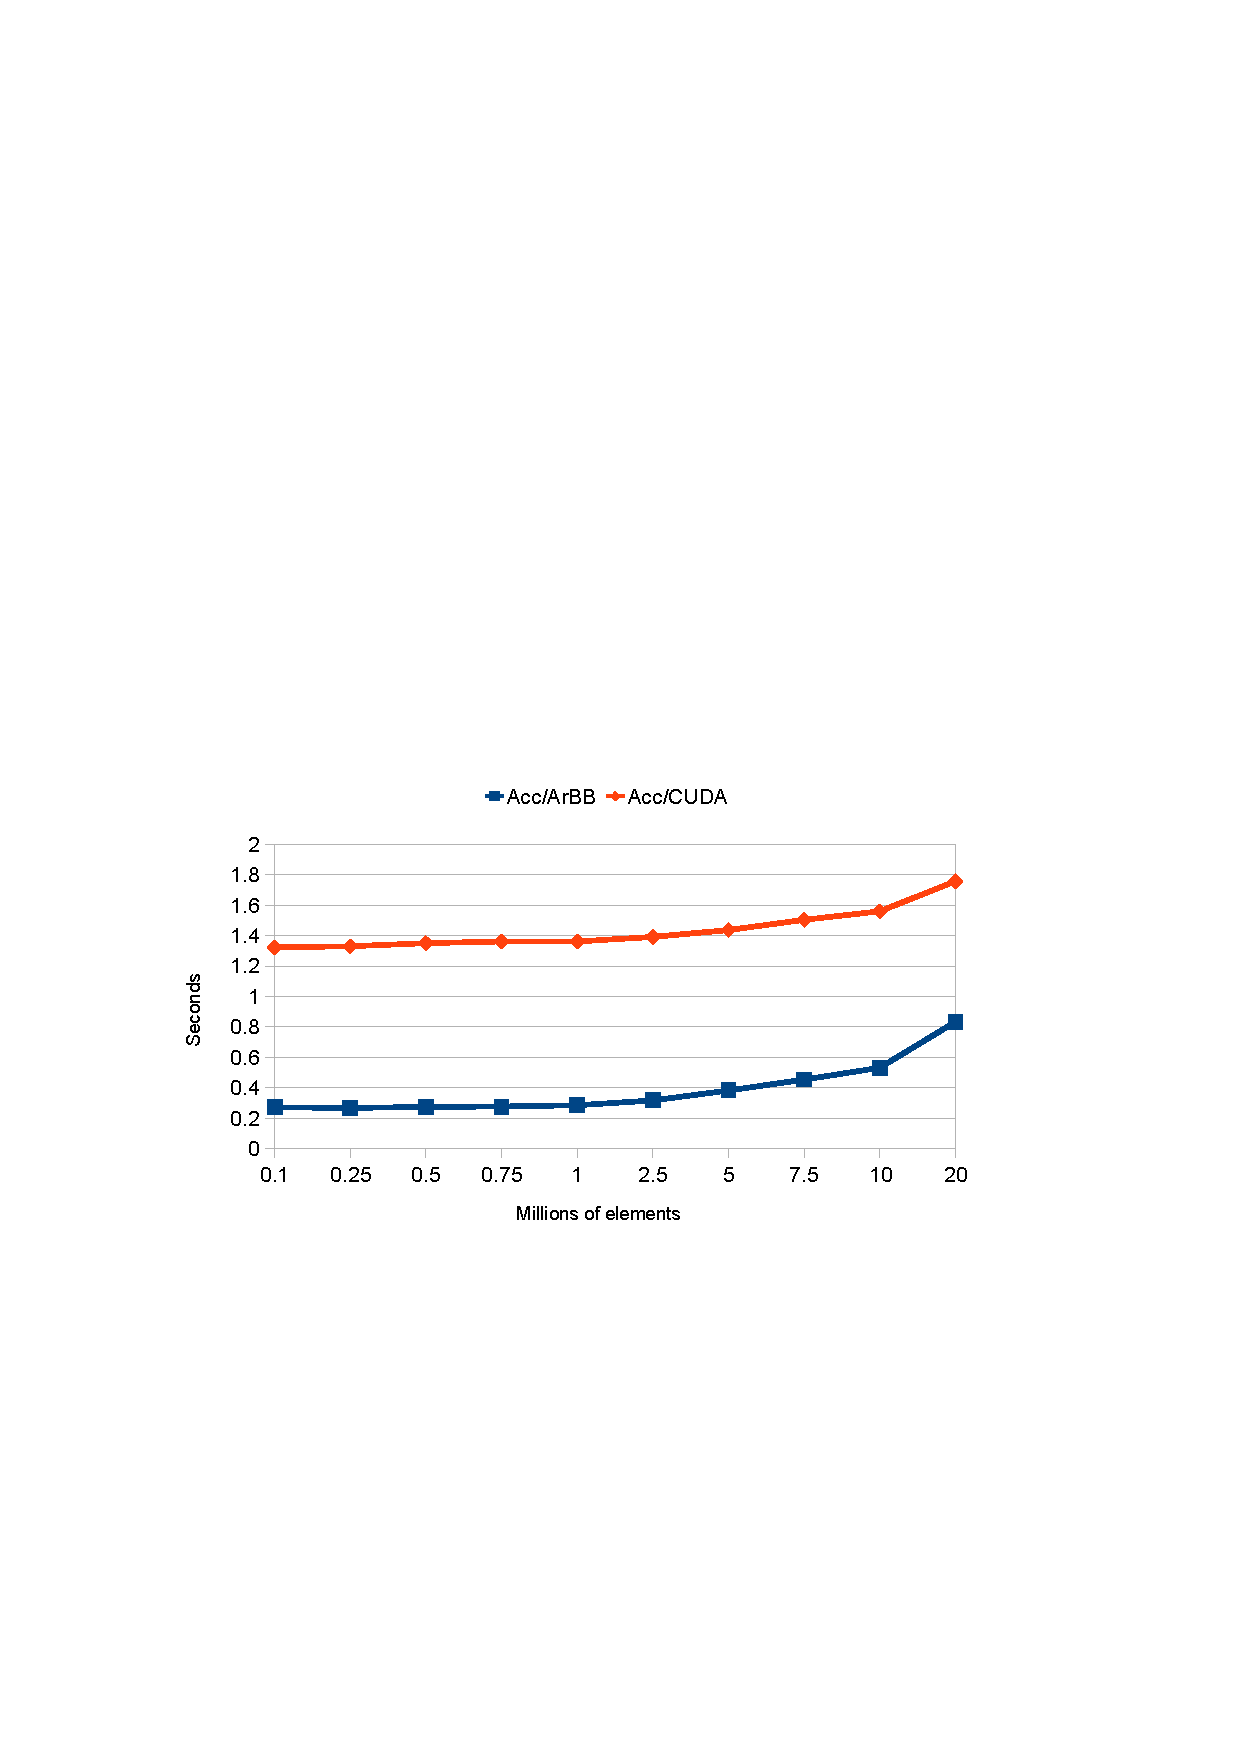
\includegraphics[width=3.5in]{./arbb/jit}    
  \end{center}
\vspace{-5mm}
  \caption{Running time experiments including JIT-time.} 
  \label{f:jit}
\end{figure}

\begin{figure}
  \begin{center}
   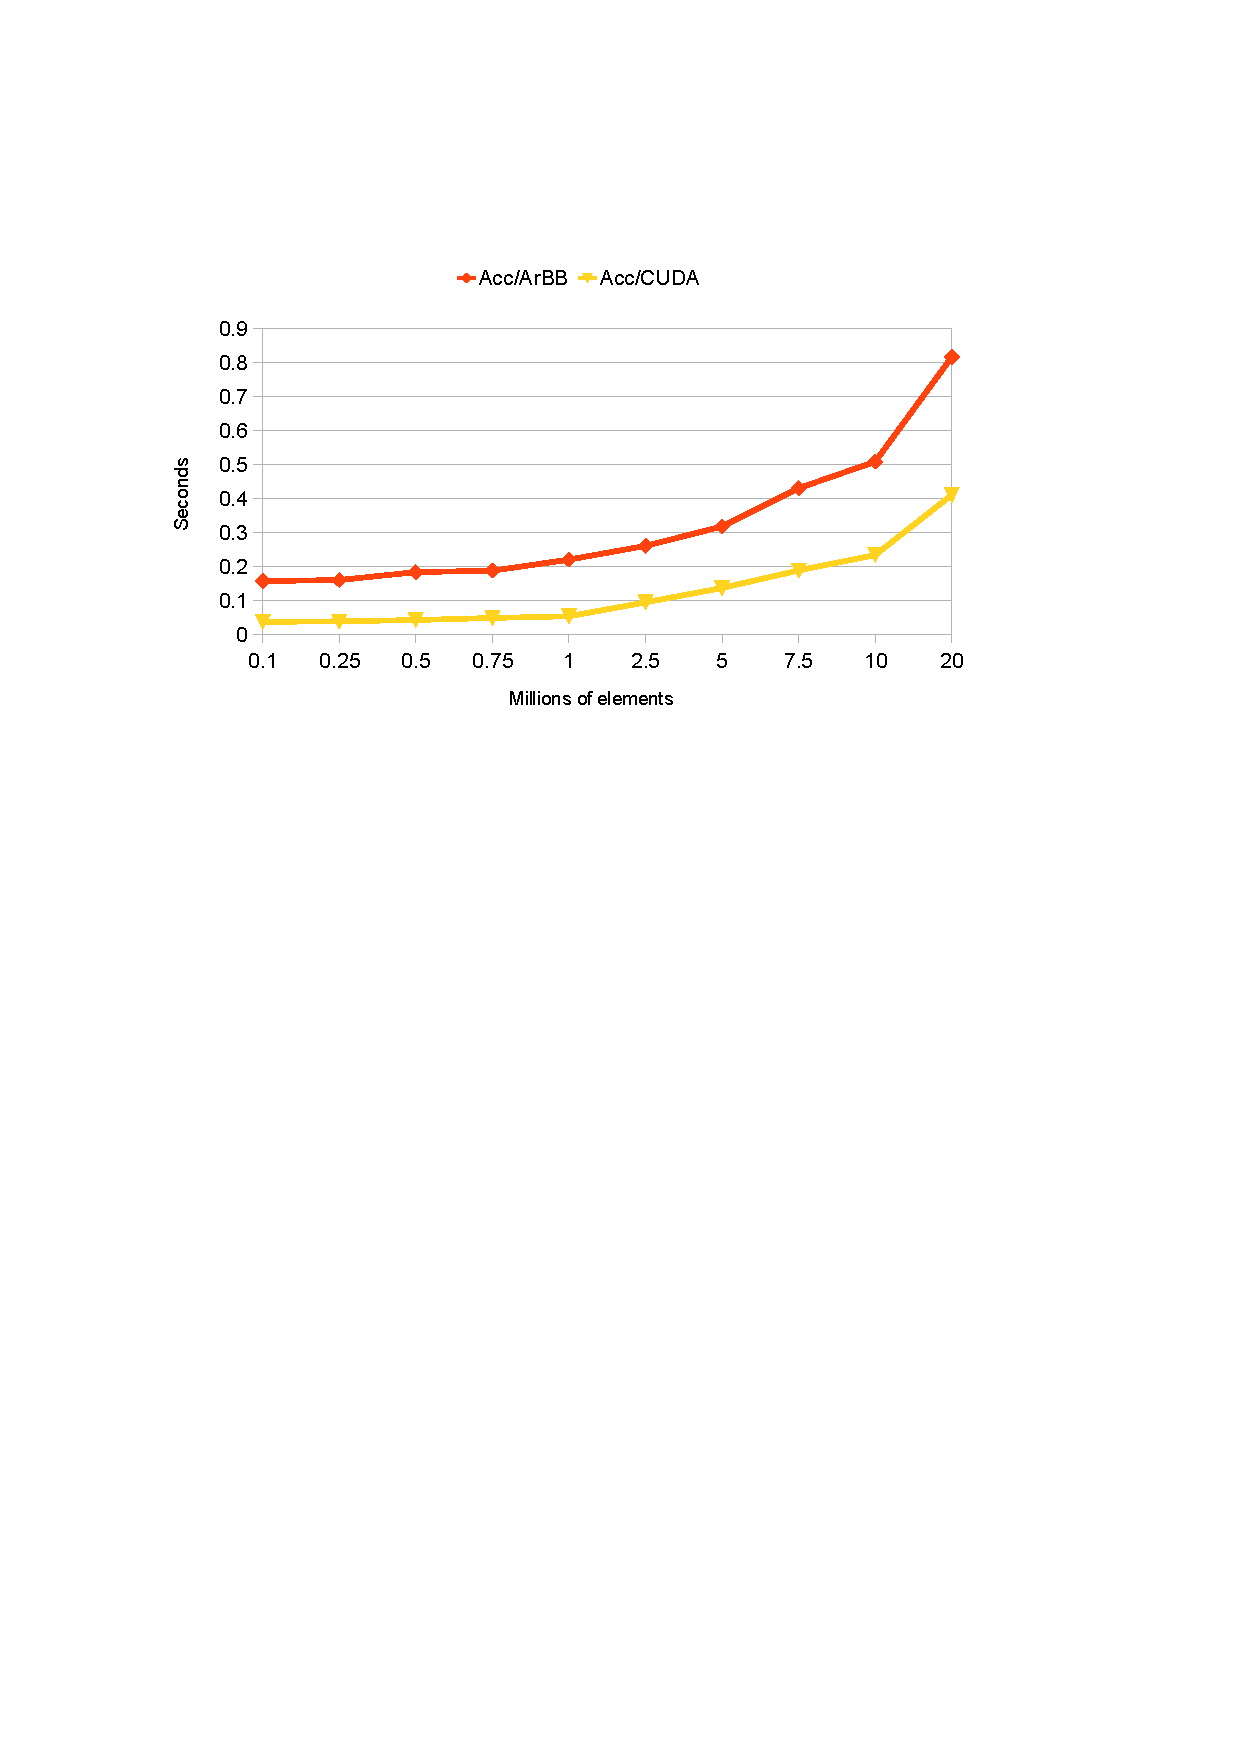
\includegraphics[width=3.5in]{./arbb/nojit}    
  \end{center}
\vspace{-5mm}
  \caption{Running time experiments JIT-time excluded.}
  \label{f:nojit}
\end{figure}


Figures~\ref{f:jit} and \ref{f:nojit} show preliminary results obtained on 
the Black-Scholes benchmark. The figures where obtained on a system with a 4-core 
Intel Core I7 975 machine with HyperThreading. The GPU used was a NVIDIA GTX480.

Figure~\ref{f:jit} shows running times obtained when JIT-time is included. 
% What this figure mainly tells us is that the JITing overhead 
JIT compilation time is much larger 
in the CUDA backend than the ArBB one.  Part of this difference 
can be attributed to the fact that 
the CUDA backend calls an external compiler (\cde{nvcc}), which takes its input in a file and runs in
a separate process.  ArBB, on the other hand, has a library interface to its  JIT-compiler. 
Figure~\ref{f:nojit} shows results obtained when pre-compiling the
CUDA functions eliminating JIT overhead.
In Accelerate, this happens automatically when the same kernel is
invoked repeatedly, because the Accelerate CUDA backed 
uses a caching scheme to avoid unnecessary JIT invocations.  (The
caching functionality has not yet been duplicated in the 
ArBB backend.)

These early results demonstrates the principle that even when a kernel
executes with higher throughput on a GPU, in a particular program it
is difficult to decide whether a computation is worth moving to a GPU,
incurring extra data-movement and possibly extra JIT compilation
\citearbb{wheres-the-data-paper}.  Specifically, we see that the
Accelerate Black-Scholes program from Figure~\ref{fig:blackscholes}
performs better on the CPU if it executes once (even on a large window
of data) whereas the GPU would yield better performance in a sustained
series of executions.
%
Because both CPU and GPU execution may be desirable---and the
selection may be dynamic---it is beneficial to have a single source code
that is portable across both.  
% Accelerate combined with \systemname{} makes this possible.


% ====================================================================================================
\subsection{Related Work}
% ====================================================================================================


OpenCL~\citearbb{opencl08} is a programming model very similar to CUDA but with the aspiration 
to offer both acceleration of computations on GPUs or to multicore CPUs. 
OpenCL JIT compiles the kernels for the particular hardware available and is
in that sense similar to ArBB.  
OpenCL programs are relatively low-level and require a large amount of
boilerplate to create and invoke.  In this sense they occupy a very
different niche than Accelerate.

Microsoft Accelerator~\citearbb{ACCELERATOR} is an embedded language with similar 
aspirations as ArBB, that is, to target a diverse range of architectures using the 
same source code. Accelerate can be used from the C\# language or the 
functional F\# language and targets GPUs or of CPUs and their
vector units.
% However, being part of the .Net framework implies limited accessibility 
%for platforms other than Microsoft Windows.  

\rn{What's the comparison with our stuff?}

%Most work on partitioning workloads between 
Many CPU and GPU comparisons, and some CPU/GPU workload partitioners \citearbb{merge}, rely on
redundant hand-written versions of all kernels
% \citearbb{cpu-gpu-partitioning} 
(though some systems like Qilin \citearbb{qilin} allow a single source code).
It is difficult in this kind of scenario
to make fair comparisons, controlling for the
amount of effort put into the respective implementations.
For example, comparing unoptimized serial CPU implementations vs. GPU
ones is not informative \citearbb{debunking-dubey}.
In \systemname{} controlling for effort
need happen only once---both CUDA and ArBB are
independently optimized by their respective teams of engineers---not for each benchmark.


% ====================================================================================================
% \section{Future work and Conclusions}
%\section{Future Work}
% ====================================================================================================

%\rn{need to be careful about being too repetitive...}
%The \accarbb{} backend is currently work-in-progress. The Accelerate
%functionality is not yet completely covered by the ArBB backend. Currently 
%the ArBB back-ed is operational for Accelerate programs using {\em Map}, 
%{\em ZipWith} and some simple instances of the Accelerate {\em Fold} operation.
%All of these also have the limitation that they only work for up to and 
%including 3-dimensional arrays using the ArBB backend while the Accelerate
%model allows the N-dimensional case. Allowing the N-dimensional case 
%in the ArBB backend for the supported operations range from a simple exercise 
%to more intricate problems needing some thought. For example, in the case 
%{\em Map} operations the needed transformation is simple (Accelerate Maps 
%over N-dimensional arrays is a per-element operation). One could flatten 
%the N-dimensional array to a 1-dimensional array (remembering its old shape) 
%perform the map and then transform the array back into N-dimensions. In 
%the case of {\em Fold} (reductions) the situation becomes more tricky. 
%transforming the arrays to arrays of lesser dimensionality then requires 
%a so-called segmented {\em Fold} operation. 

%The current \accarbb{} backend uses a hybrid of immediate-mode 
%and retained-mode programming styles. Moving more towards 
%retained-mode only may have performance benefits since it would give the 
%ArBB compiler larger programs to optimize. Exploring this aspect is left 
%as future work. 

% ====================================================================================================
\subsection{Discussion and Conclusions}
% ====================================================================================================

We have demonstrated that an EDSL such as Accelerate is sufficiently
platform-independent to break free of its original hardware target
(CUDA/GPU) and create efficient programs on other architectures.  This
gives us hope that \systemname{}/Accelerate programs will be
forward-portable to future parallel architectures and instruction
sets.

The EDSL approach changes the playing field for the designer
of compiler backends.  Rather than contending with full blown
languages and their complexities (e.g. pointers, aliasing,
inheritance, virtual functions, etc), compiler backends can focus on
simple value-oriented compute languages.

%% Achieving the ultimate goal of performance portability requires
%% progress on two research problems.  The first is EDSLs themselves and
%% their integration into host languages.  The second problem 

But the EDSL method solves only part of the performance-portability problem.
Simple as EDSL target languages may be, there remains a
substantial challenge in mapping them efficiently to the diversity
of parallel architectures available now and in the near future.
%especially without requiring a large amount of additional per-platform
%user annotations.
\textred{For example, the idiosyncrasies of memory bank access on
  NVIDIA GPUs must be taken into account to generate efficient
  implementations of the high-level collective operations that we have
  discussed.}

This is a compiler backend research challenge.
The {\em skeletons} method mentioned in
Section~\ref{sec:accelerate-arbb} is one approach to this problem, as
are the optimizations studied in the Copperhead \citearbb{copperhead} and
Obsidian \citearbb{JSLIC} projects.
%
On the other hand, systems that rely on advanced optimizations
typically suffer to some extent from performance-predictability
problems.  Thus achieving portable, predictable performance on a wide range
of architectures---even for the simplest target languages---will
be the subject of much future work.

%{
%\small
\bibliographystylearbb{alpha}
\bibliographyarbb{thesis}
%}


%\end{document}




% ---------------------------------------------------------------------------
% 
% ---------------------------------------------------------------------------
\cleardoublepage 

\section[\paperETitle]{\paperE: \\ \paperETitle}
\label{sec:paperE}
%\addcontentsline{toc}{chapter}{Counting and Occurrence Sort for GPUs using an Embedded Language}

% \paperETitle

\begin{center} 
Josef Svenningsson, Bo Joel Svensson, Mary Sheeran 
\end{center}



%% bare_conf.tex
%% V1.3
%% 2007/01/11
%% by Michael Shell
%% See:
%% http://www.michaelshell.org/
%% for current contact information.
%%
%% This is a skeleton file demonstrating the use of IEEEtran.cls
%% (requires IEEEtran.cls version 1.7 or later) with an IEEE conference paper.
%%
%% Support sites:
%% http://www.michaelshell.org/tex/ieeetran/
%% http://www.ctan.org/tex-archive/macros/latex/contrib/IEEEtran/
%% and
%% http://www.ieee.org/

%\documentclass[conference]{IEEEtran}

%\usepackage{graphicx, color, code}
%\usepackage[cmex10]{amsmath}
%\usepackage{url}
% \usepackage{bookman}  %% bold teletype fonts, but don't know how to prevent it from changing the whole document

% Haven't figured out how to get this to work properly:
%\usepackage[\texttt{cmbtt}]{bold-extra}
% \usepackage{bold-extra} 

%\usepackage{courier}
%\usepackage{fancyvrb}

% correct bad hyphenation here
%\hyphenation{op-tical net-works semi-conduc-tor}


%====================================================================================================
%% FIRST, MISC USEFUL DEFINITIONS
%====================================================================================================

\definecolor{darkgreen}{rgb}{0, 0.5, 0}
\definecolor{darkblue}{rgb}{0,0,0.5}
\definecolor{mygrey}{rgb}{0.7,0.7,0.7}
\newcommand{\textblue}[1]{\textcolor{blue}{#1}}

\newcommand{\cde}[1]{{\footnotesize \tt #1}}

% \newcommand{\kw}[1]{{\bf{#1}}}
\newcommand{\kw}[1]{{\textbf{#1}}}

\newcommand{\comm}[1]{{\em \textcolor{darkgreen}{#1}}}  %% Code comments

\newcommand{\note}[1]{\begin{itemize}\item \textcolor{blue}{#1} \end{itemize}}

%% \newenvironment{mycode}
%% {% This is the begin code
%%   \begin{Verbatim}[commandchars=\\\{\}]}%
%%   %\footnotesize
%%   %\noindent
%%   %\begin{code}\noindent\vspace{-1mm}}
%% %  \begin{code}\noindent}
%% {% This is the end code
%%   \end{Verbatim}
%%   %\end{code} 
%% }

%% \newenvironment{inlinecode}
%% {
%%   \begin{center}
%%   \begin{minipage}{4in}
%%   \begin{mycode}
%% } 
%% {
%%   \end{mycode}
%%   \end{minipage}
%%   \end{center}
%%   \vspace{-1.5ex}
%% }

%% ============================================================
%% USE TO DISABLE COMMENTS:
 \def\noeditingmarks{}
%% ============================================================
\ifx\noeditingmarks\undefined
   \newcommand{\textred}[1]{\textcolor{red}{#1}}
   \newcommand{\pgwrapper}[2]{\textred{#1: #2}}
%   \newcommand{\pgwrapper}[2]{}
   \newcommand{\rnote}[1]{\begin{itemize}\item{\textcolor{blue}{#1}}\end{itemize}}
   \newcommand{\new}[1]{\textcolor{blue}{#1}}
   \newcommand{\const}[1]{\textred{#1}}

%% RRN: Dim the background for Ryan's eyes:
%%   What I need here is a way to do it based on user or host name...
% \pagecolor{mygrey}

\else
   \newcommand{\textred}[1]{#1}
   \newcommand{\pgwrapper}[2]{}
   \newcommand{\rnote}[1]{}
   \newcommand{\new}[1]{#1}
   \newcommand{\const}[1]{#1}
\fi

\newcommand{\js}[1]{\pgwrapper{BJS}{#1}}
\newcommand{\rn}[1]{\pgwrapper{RRN}{#1}}


%% Can we call our ``things'' 
%% ArBB/Haskell for the bindings part ? 
%% Accelerate/ArBB for the Accelerate backend ?
%% This would work with the convention we adopted for 
%%      ArBB/C++  
\newcommand{\systemname}[0]{{Harbb}}
%\newcommand{\systemname}[0]{\textred{HArBB}}

%% This could in theory be separate from the project name..
\newcommand{\accarbb}[0]{\systemname{}}

%% NOTE: THIS SHOULD BE THE SAME AS SYSTEMNAME:
\newcommand{\arbbvmH}[0]{ArBB/Haskell}


%====================================================================================================
% END DEFINITIONS
%====================================================================================================




%\begin{document}
% \title{Painless Portable Vector Parallelism\\ with Haskell and Intel ArBB}
%\title{Programming Future Parallel Architectures\\ with Haskell and Intel ArBB}
% \title{Embedded Domain-Specific Languages Pave the Way for New Parallel Architectures}

%\author{\IEEEauthorblockN{Bo Joel Svensson}
%\IEEEauthorblockA{Dept. of Computer Science and Engineering\\
%Chalmers University of Technology\\
%Gothenburg, Sweden\\
%Email: joels@chalmers.se}
%\and
%\IEEEauthorblockN{Ryan Newton}
%\IEEEauthorblockA{Intel Corporation\\
%Hudson, MA\\
%Email: rrnewton@gmail.com
%}}
% Email: ryan.r.newton@intel.com

%\maketitle

%\begin{abstract}
%
\subsection*{Abstract}
New parallel architectures, such 
\new{as Cell, Intel MIC, GPUs, and tiled architectures, enable} high
performance but are often hard to program.
What is needed is a bridge between high-level programming models 
where programmers are most productive and modern parallel architectures. 
We propose that that bridge is Embedded Domain Specific Languages (EDSLs). 

\new{One attractive target for EDSLs is}
Intel ArBB, a virtual machine for parallel, vectorized computations.
% that serves as a compilation target for EDSLs.
We propose to wed ArBB with the functional programming language
Haskell, {using an EDSL} that generates code for the ArBB VM.  This Haskell integration provides 
% a determinism guarantee 
added safety guarantees compared to other ArBB interfaces.
%
Further, our prototype, \systemname{}, is one of the first EDSL implementations with
optimized backends for multiple parallel architectures (CPU, \new{NVIDIA GPU}, and
others), allowing portability of source code over devices
and their accelerators.


%\end{abstract}
%\IEEEpeerreviewmaketitle




% ====================================================================================================
\subsection{Introduction}
% ====================================================================================================

Are radical new parallel architectures market-feasible if they require
significant changes for programmers?  The jury is out.  In recent
years we have seen difficult-to-program chips suffer 
% \citearbb{cell} 
(e.g. Cell)
and
GPU vendors strive to enable more traditional programming features
\citearbb{fermi} (e.g. C++).  There is an increasing
tension between ease of programming and efficiency.

The tension  shows  across diverse chip markets.  For example,
small embedded devices are most power efficient if their processors and operating systems
omit programming features such as virtual memory and threads \citearbb{tinyos}.  
At the other end of the power spectrum, GPU's
graphics performance may suffer due to inclusion of hardware to ease
GPGPU programming.  In short, there is an opportunity cost to
including extra hardware for programmability.

In this paper, we argue 
that a specific technique holds the greatest promise of solving the programmability dilemma.
%
Domain-specific languages, {\em embedded} within general purpose
languages (EDSLs) 
 enable familiar programming models 
{\em and} flexible
mapping onto new hardware.  The key to having this cake and eating it
too is {\em metaprogramming}.  Familiar programming features are
present, but are eliminated at an intermediate (metaprogram evaluation)
phase and therefore do not reach the parallel hardware itself.


% We present our ongoing work on a
In pursuit of this vision, we offer a
% 
 new EDSL implementation, called \accarbb{}, that combines
existing systems, Accelerate \citearbb{ACCELERATEDAMP11} and ArBB \citearbb{ArBB}, to produce a unified
high-level programming environment equally suited to multicore,
vectorized CPUs, as to GPUs and other accelerators (such as Intel MIC chips \citearbb{larrabee}).
%
\if{0}
ArBB is based on the RapidMind \citearbb{RapidMind} system which was an embedded 
DSL targeting multicore CPUs as well as GPUs. ArBB does not \new{yet} include a GPU 
backend like RapidMind, targeting multicore CPUs and their vector 
units. 
\fi{}
\systemname{} is a single EDSL implementation 
with independently optimized backends \new{by different teams; 
namely, the ArBB backend for CPU/MIC, and a CUDA backend for NVIDIA GPU.}
This makes
\systemname{} an appealing platform for fair CPU/GPU comparisons, 
as well as a compelling programming model for single-source portable performance across a range of
parallel architectures, \new{present and future}.
%%To our knowledge, \systemname{} is the first EDSL implementation with
%%independently optimized backends for CPUs and GPUs.  This makes
%%\systemname{} an appealing platform for fair CPU/GPU comparisons, 
%%as well as a compelling programming
%%model for single-source portable performance across a range of
%%parallel architectures.


% ====================================================================================================
\subsection{Embedded Domain-Specific Languages}
% ====================================================================================================


Domain-specific languages---from Makefiles and \LaTeX{} to
Matlab---are almost too ubiquitous to notice.  Most relevant to our
purposes, domain-specific languages (DSLs) that target a narrow domain and expose communication
patterns to the compiler 
 have achieved performance-portability across a wide range of parallel
architectures.  
StreamIt\citearbb{streamit} is a good example.
% (for example, StreamIt\citearbb{streamit})
% The high-water mark in this area is perhaps  StreamIt\citearbb{streamit}.
% 

% It has been noted \citearbb{not-sure} that 
% Yet the few DSLs that gain popularity lose simplicity\citearbb{not-sure}.  
% Yet popular DSLs rarely remain simple \citearbb{not-sure}.  
DSLs may start out simple and focused, but if they gain popularity
they quickly grow in complexity to rival full-blown languages.
Feature creep
can make DSL implementations complex and expensive to maintain.
Further, non-standard DSL syntax and features present a learning curve for users.  In the
last ten years an attractive solution to this dilemma has emerged: {\em
  embed} each DSL into a general-purpose host language that can provide
common functionality with familiar syntax and semantics.
% in place of the DSL.

When embedding, host language programs {generate} DSL programs;
% Embedding means that the host language is used to generate DSL programs; 
the {\em deeper} the embedding, the more integrated the
DSL into the syntax and type-system of the host language.
%
% Typically, %% pruning weasel words
A key host-language feature for embedding is that
language constructs can be overloaded to operate over {\em abstract
  syntax trees} (ASTs)\footnote{This ad-hoc polymorphism is accomplished,
for example, through operator-overloading in C++ or type classes in
Haskell.}.  For example, the following simple function operates on scalars:


\vspace{1mm}
\begin{Verbatim}[commandchars=\\\{\}]
  float f(float x) \{ return (2*x - 1); \}
\end{Verbatim}
\noindent
But simply by changing the types, \cde{f} might be lifted to operate on {\em
  expressions} (which, when evaluated, will yield \cde{floats}):

\vspace{1mm}
\begin{Verbatim}[commandchars=\\\{\}]
  \kw{exp<float>} f(\kw{exp<float>} x) \{
    return (2*x - 1);
  \}
\end{Verbatim}

A common arrangement is for the host language program to execute at
runtime but to generate ASTs that are executed by a just-in-time
(DSL) compiler.  This use of metaprogramming (program generation)
differs from the more common usage of preprocessors and 
% Lisp/Scheme macros \citearbb{scheme-macros}
macros, which typically add extra
phases of computation {\em before}  compile time---increasing
the number of compile-time rather than runtime phases.

% EDSLs typically add additional runtime phases.  That is, the host language program 
% executes at runtime but uses a JIT to process generated ASTs.
%% which are
%% usually used to perform computation {\em earlier} than the usual
%% compile time, embedded DSLs (EDSLs) typically defer computation 


One reason that EDSLs are good for productivity is that the programmer
gains the software engineering benefits of the host language
(object-orientation, higher-order-functions, modules, etc), while not
paying the cost at runtime for additional layers of abstraction or
indirection.  Indeed, the embedded languages for 
performance-oriented EDSLs are often simple, first-order
languages without pointers \citearbb{wavescript, ACCELERATEDAMP11}.

% , paul-lius-thingy

% regiment,
As a research area, EDSLs and two-stage DSLs have been actively pursued for at least a
decade \citearbb{VERTIGO, wavescript} but are gaining steam
recently 
%\citearbb{sejits, stanford-ppl} 
\citearbb{copperhead, stanford-ppl} 
and are beginning to appear in
commercial products \citearbb{ArBB}.
%
Further, EDSL techniques have spread beyond their origin in 
 the programming languages community.
% 
For example, both Stanford's Parallel Programming Laboratory (PPL) and
the Berkeley Parlab are creating EDSLs as their flagship parallel
programming solutions for domains such as machine learning and
rendering \citearbb{stanford-ppl}.
  Moreover, EDSLs need not be hosted by esoteric research languages---Intel's
 ArBB embeds an array language in C++ and Berkeley's
Copperhead \citearbb{copperhead} generates CUDA from simple Python code.

%\rnote{Is there a good motivating example program?  What are some of
%  the Metaocaml motivating examples?}

{For the remainder of this paper we will focus our discussion
  on the Intel ArBB VM, a virtual machine for just-in-time
  generation of vector codes, \new{which implements a restricted} domain-specific
  language of array computations.  In this paper we introduce
  {\em High-level ArBB}, 
  (\systemname{}), an EDSL that internally uses the ArBB
  VM.  \new{While Intel's ArBB package already includes an EDSL targeting the VM (for C++)},
\systemname{} \new{offers additional advantages, including}
  more succinct programs and additionally safety
  guarantees---namely, complete deterministic-by-construction parallel
  programs (across both host and VM languages).}


% ====================================================================================================
% \section{Accelerate and ArBB}
%\section{\accarbb{}:  ArBB and Accelerate}
\subsection{\accarbb{} $=$ ArBB $+$ Accelerate}
\label{sec:accelerate-arbb}
% ====================================================================================================

Our first \systemname{} prototype adapts an existing EDSL called {\em
  Accelerate} (Data.Array.Accelerate).  Accelerate targets high-level
data-parallel programming in Haskell.
Previous work on Accelerate has focused on developing a CUDA-backend
for GPU programming.  In this paper we describe our effort to retarget
Accelerate to ArBB.  

With respect to determinism guarantees, the existing Intel ArBB product
represents an integration of the safe (ArBB VM) with the unsafe (C++).
In the Haskell context, because purely functional computations are
guaranteed deterministic (even when executed in parallel), and because
ArBB computations invoked by Haskell functions are themselves free of
side-effects, \systemname{} achieves a
guarantee of determinism for complete programs that combine both
Haskell computation and ArBB VM computation.
% which offers portability.
% (The 'H' in \systemname{} therefore stands for Haskell as well as ``High-level''.)


%% {\em Accelerate} (Data.Array.Accelerate) is an existing EDSL for 
%% high-level data-parallel programming in Haskell~\citearbb{Accelerate}. 
The Accelerate programming model consists of collective 
operations that can be performed over arrays, together with a simple 
language of scalar expressions\new{---in the current release, the Haskell type system enforces that parallelism not be nested.}
\if{0}
The Haskell type 
system is used to enforce that no nested data-parallelism can be expressed 
\new{(in the current release, this may be relaxed in the future).}
\fi{}
Accelerate's collective operations include {\em Map} (akin to parallel
for loops) {\em ZipWith} (a generalization of elementwise vector addition) and 
{\em Fold} (sum generalized)---familiar operations for programmers versed in the functional paradigm.
All of these collective operations are easily parallelizable. 
% In the case of {\em Map} and {\em ZipWith} the potential for parallelism is abundant.  

%% dotProd :: Vector Float -> 
%%            Vector Float -> 
%%            Acc (Scalar Float) 
\begin{Verbatim}[commandchars=\\\{\}]
dotProd (xs :: Vector Float) 
        (ys :: Vector Float) = 
  \kw{let} xs\_ = use xs 
      ys\_ = use ys 
  \kw{in}  fold (+) 0 (zipWith (*) xs\_ ys\_) 
\end{Verbatim}

The Accelerate code listing above specifies a function that takes two 1-dimensional 
arrays as inputs (of type \cde{Vector Float}, e.g. a vector of floats). The result of the function is a single
scalar. 
% (\cde{Scalar Float})
The \cde{use} function is applied to an array to convert it 
for use in the collective operations provided by Accelerate;
\cde{use} 
% is actually a function with type \cde{Vector a -> Acc (Vector a)} and 
may result in
copying the array to, for example, the GPU in the case of Accelerate's 
CUDA backend.  

After applying \cde{use} to bring in input data, the programmer then
constructs a data-parallel program from collective operations.
Above, \cde{fold} is a function that takes three arguments, 
here those arguments are \cde{(+)},  $0$ and \cde{zipWith (*) xs\_ ys\_}. 
\cde{zipWith}, in turn, is a function taking three arguments, \cde{(*)}, 
\cde{xs\_} and \cde{ys\_}. The \cde{zipWith} operation here applies pairwise 
multiplication to the two arrays and the \cde{fold} sums up all the elements 
into a single scalar. 

%\rn{Following para slightly redundant but ok...}
%Accelerate makes GPU programming accessible to the functional programmer 
%by offering a familiar set of operations. This set of operations also have 
%the beneficial property that they have inherent parallelism and are 
%easily implementable on the GPU. 

Accelerate's CUDA backend implements collective operations using
a hand-tuned ``skeleton'' for each operation (and possibly for
different hardware versions). The kernel---for example, the function
to mapped over the dataset---is 
instantiated into the body of the skeleton code. The resulting 
program is compiled using the NVIDIA CUDA compiler and dynamically linked 
into the running Haskell program.

%\subsection{Intel Array Building Blocks (ArBB)}
\subsection{Intel Array Building Blocks (ArBB)}
\label{sec:arbb}

%ArBB is embedded in the C++ programming language but it also exposes a 
%very low level API that is purely C. 
%{\em ArBB} (Array Building Blocks) is also an embedded DSL. 
The operations exposed by ArBB are similar to those of Accelerate. 
In ArBB, parallel computations are expressed using a set of built-in 
primitives. All vectorization and threading is managed internally by 
ArBB. The programmer uses collective operations with a clear semantics 
such as \cde {add\_reduce} that computes the sum of the elements in a given 
array. ArBB also has language constructions for control flow, conditionals
and loops. These operations have their usual sequential semantics and are not 
parallelized by the system, rather, only specific collective operations are executed
in parallel. 

Today's existing ArBB product is embedded in C++ and provides special
types for scalars and arrays (e.g. \cde{dense<f32>} rather than \cde{vector<float>}).
Using ArBB/C++ to express the dot product computation can be done 
as follows:

%\vspace{2mm}
\begin{Verbatim}[commandchars=\\\{\}]
\kw{void} dot\_product(\kw{const} dense<f32>& a, 
                 \kw{const} dense<f32>& b,
                 f32& c) 
{ 
  c = add\_reduce(a * b);
}
\end{Verbatim} 


% The above program takes two arrays of type \cde{dense<f32>} as input. 
% \cde{dense<f32>} specifies a 1-dimensional array of 32-bit floating
% point values. The result is a single 32-bit float.  

Note that arithmetic operators such as (*) are overloaded 
for to operate on arrays as well as scalars (e.g. \cde{a * b} above).
Thus, the above C++ function multiplies two arrays before summing them with \cde {add\_reduce}:

The code listing below is indicative to the amount of glue code needed to invoke an 
ArBB computation\footnote{In OpenCL and CUDA the glue code situation is even worse}. It shows how the dot product code is launched using {\tt call} and 
how data is bound, {\tt bind}, for use in ArBB. 

\vspace{2mm}
\begin{Verbatim}[commandchars=\\\{\}]
\kw{int} main() 
\{ 
  double a[SIZE];
  double b[SIZE];

  for ( \kw{int} i = 0; i < SIZE; ++i) \{ 
    a[i] = ...; b[i] = ...;
  \}
  dense<f32> va, vb;
  f32 vc;
  bind(va, a, SIZE); 
  bind(vb, b, SIZE); 
  call(dot\_product)(va, vb, &vc); 
  ...
\}
\end{Verbatim}


%\rnote{SPECIFICALLY ADDRESS THE FUNCTIONALITY GAP?  E.G general
%  reduce.  Any other examples?}

The model provided by Accelerate is slightly richer than that of ArBB.
Even the two very simple \cde {dot\_product} examples above manage to illustrate 
this. In Accelerate there is a more general reduction primitive called \cde {fold} 
where in ArBB there are specific reductions, \cde {add\_reduce}, \cde {mul\_reduce} 
and so on. Not visible in these small examples is another difference, Accelerate 
operations are generalized to arbitrary dimensions while ArBB operations are 
limited to 1, 2, and 3 dimensions (and 0, i.e. scalar). These differences aside,
the ArBB and Accelerate programming models are very similar.


% ====================================================================================================
\subsection{Implementation of \systemname{}} 
% ====================================================================================================


%\rnote{Sadly the Haskell details don't buy us much here... what are
%  the {\em conceptual} problems solved in mapping the Accelerate
%  abstraction to the ArBB one?  The data models are similar, but
%  there are always mismatches -- dimensionality support, missing
%  reduction.}

%\rnote{What is the technique that you are using to address these sorts
%  of problems?  Is there anything to say about it?}

\begin{figure}
  \begin{center}
   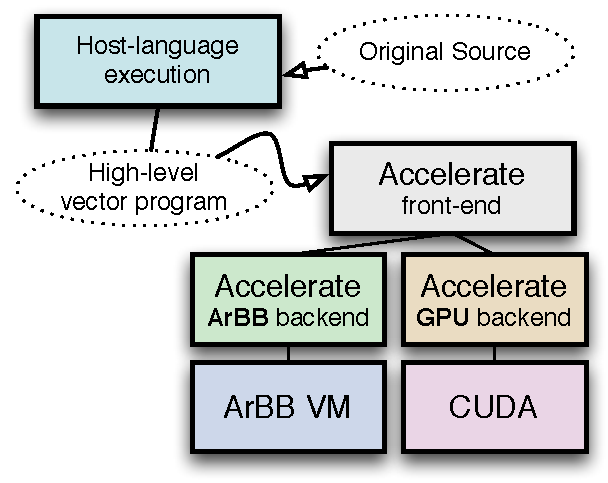
\includegraphics[width=2.0in]{./arbb/figure_architecture}    
  \end{center}
\vspace{-5mm}
  \caption{Architecture of the \systemname{} system.  \rn{(ROUGH.)}}
  \label{f:architecture}
\end{figure}


Using Accelerate and ArBB together, we propose a layered architecture
for \systemname{},
% Our goal is to make the benefits of ArBB available to the Haskell programmer. 
% \js{(Or is our goal to give an even better ``front-end'' to ArBB compared to C++)}
% We propose that this is best accomplished using a layered approach, as
pictured in Figure~\ref{f:architecture}. 
The host language execution (via Haskell in this case) executes the
programmer's source code, generating a vector program in the
restricted language of the Accelerate front-end.
Then either Accelerate backend---ArBB or CUDA---may be used.
The 
bottom layer of the ArBB backend consists of a direct mapping of the ArBB virtual machine
API (VMAPI) into Haskell including one-to-one bindings for each C 
function. 
To [partially] automate the creation of these bindings we used the C2HS system \citearbb{C2HS}. The 
\arbbvmH{} bindings are very low-level.
%and make little use of the high-level programming methods that
% Haskell programmers want. 
The idea 
is that the \arbbvmH{} bindings should be used to implement
backends for higher-level data-parallel EDSLs.

%% To illustrate our position we 
%% have started working on a backend to the successful DSL Accelerate 
%% (Data.Array.Accelerate) using our \arbbvmH{} bindings. 

To address the functionality mismatch between Accelerate and ArBB,
when possible we reencode the users Accelerate program using existing
ArBB mechanisms.  Our prototype does not support 100\% of Accelerate's
compute model (for example, only supporting  up to three-dimensional
arrays), but the remaining functionality can be mapped onto ArBB in
time using known methods---for example, our compiler could map higher
dimensional arrays onto a specific lower-dimensional data-layout.

%% The programming models supported by ArBB and Accelerate are very similar. 
%% Both obtain their parallelism by exposing collective operations 
%% such as {\em Map}, {\em Reduce}, {\em ZipWith} and {\em Scan} (all prefixes operations). However, 
%% the functionality match is not 100\%. For example, Accelerate supports {\em Map} operations 
%% over N-dimensional Arrays while ArBB supports them only up to 3-dimensions. 
%% Similar inconsistencies apply to the other operations as well. \textred{The current
%% ArBB backend simply disallows Accelerate programs using too high dimensionality
%% of the arrays.} \rn{Sure, we want to say that we're not done closing
%%   this gap (for
%%   accuracy) but more importantly we want to identify whether
%%   techniques exist to close the gap.  Presumably, yes?  We can
%%   ourselves collapse the dimensionality of arrays before giving them
%%   to ArBB?  Are there any operations that would defeat that technique?}
%

One example of a functionality discrepancy bridged by our
implementation is reductions.  As mentioned in \ref{sec:arbb},
Accelerate allows the programmer to reduce using an arbitrary
associative function, but ArBB has only built-in reductions with fixed
operations (add, multiply, xor, etc). We plan to provide general reductions in
the ArBB backend by a two-fold strategy:

\begin{enumerate}
\item Attempt to map an Accelerate reduction directly onto an ArBB
  primitive such as \cde{add\_reduce}.
\item Apply a general reduction technique based on $log(N)$ map
  operations over successively halving array sizes.  Essentially, cut
  the array in half, combine the halves, repeat. In ~\citearbb{reduction}
  this approach is explained in the context of CUDA. 
\end{enumerate}

%% \rn{Is the technique worthy of
%%   description?  Can we just cite the CUDA documentation or something
%%   since it's common?} 

In our current experiments, approach (2) is significantly slower.
Therefore, the ideal would be that ArBB exposed general reduction
directly in its programming model.  We expect this functionality to be
added in future releases.  In the meantime we plan to explore a
technique that would allow us to maximize the number of situations in
which (1) above applies.  Namely, a reduce operation can often be {\em
  factored} into a map followed by a reduce.  For example, a reduction
that multiplies each input number by a coefficient and sums the
results can be split into a map phase for the multiplication followed
by the built-in \cde {add\_reduce} operator.

%% Currently, our reduction implementations in ArBB 
%% are many times 
%% slower (\textasciitilde 20x) than their built-in counterparts. 
%% % To ameliorate this present performance problem we attempt to map
%% % programmers 
%% Our present workaround for this performance problem is to let 
%% \accarbb{} inspect the reduction function and switch to efficient 
%% built in  ArBB reduction where possible.  
%% \rn{Future work may be to decompose reductions into map+reduce so as
%%   to allow the reduce to become a builtin.}


Another choice faced by our implementation is the granularity at which the
ArBB JIT is invoked.  Specifically, should each collective operation result in its
own call to the ArBB JIT (in ArBB terminology, {\em
  immediate-mode}, akin to the pre-OpenGL 3.0 immediate mode), or
should multiple collective operations be placed together
inside an ArBB function and passed to the JIT?
We will call the latter approach {\em retained-mode}.

%% In immediate-mode the 
%% operations called from the ArBB API are executed
%% synchronously---before each API call returns. In retained-mode, ArBB
%% collects calls and, only when results are requested, the 
%% entire computation is optimized 
%% and executed. 

Retained-mode generally offers performance benefits; a bigger 
chunk is given to the JIT compiler, enabling cross-optimization
between collective operations. 
Our prototype Accelerate backend uses 
ArBB in  
a combination of immediate- and retained-mode. The main collective 
operations are compiled using the retained-mode. For example, in the case 
of a \cde{map f}  operation first the function to be mapped is created and 
compiled using retained-mode then a small {\em mapper} function is 
also created and compiled using retained-mode. 
%% The mapper function is 
%% of course very small and therefore does not give much to the JIT compiler 
%% to work on optimization-wise. 
Between the collective operations the backend
needs to perform data management and copying, which 
are performed in immediate-mode. It is our belief that 
\systemname{} would benefit from using retained-mode exclusively 
but we leave that as future work. 





% ====================================================================================================
\subsection{Preliminary Results}
% ====================================================================================================

%\rnote{One tiny benchmark if we can manage it.}

%\rnote{Ideally: Something like blackscholes running Arbb/C++,
%  \systemname{}, CPU+GPU, possibly compared to other blackscholes
%  implementations -- say Cilk on CPU and hand-coded CUDA (I can
%  provide the former I think).  Perhaps serial, non-vectorized CPU for
%  comparison.}

%\rnote{Point 1 -- High level thing is within X\% of low level thing.
%  The usual.  But we also want to say that \systemname{} is no worse
%  than ArBB/C++ -- the metalanguage doesn't matter, be it Haskell,
%  Python, or C++.}

%\rnote{Point 2 -- It's important to do a good job on the CPU side.
%  Even if you don't beat GPU there's a big difference between
%  vectorizing/not-vectorizing (and using multicore of coarse).  Can't
%  be ignored.}

%\rnote{Bonus points -- if we could show how bad ``naive'' ports are that
%  would be nice.  How well does your C CPU code run on GPU unmodified
%  (or minimally ported)?}



%\rnote{CPU/GPU systems that do a good job of both.  Perhaps quickly
%  dismiss those that make no effort on the CPU side.}

Black-Scholes option pricing is a finance-related benchmark that has been used in similar
DSLs targeting GPUs \citearbb{ACCELERATEDAMP11, NIKOLA}. Since we are re-using the 
Accelerate front-end, we can directly use the Black-Scholes benchmark that 
is shipped with that system.  Figure \ref{fig:blackscholes} shows the
complete code listing for an Accelerate Black-Scholes function which
can be executed on GPUs or any processor targeted by ArBB.

% blackscholes :: Vector (Float, Float, Float) 
%
%                -> Acc (Vector (Float, Float))
%\fbox{

%       r     = \textit{constant} riskfree
%       v     = \textit{constant} volatility

\begin{figure}
\begin{footnotesize}
\begin{Verbatim}[frame=single, commandchars=\\\{\}]
blackscholes (xs :: Vector (Float,Float,Float)) = 
  map kernel (\textit{use} xs)

kernel x =
  \kw{let} (price, strike, years) = \textit{unlift} x
      r     = 0.02 \textsf{\textit{-- riskfree constant}}
      v     = 0.30 \textsf{\textit{-- volatility constant}}
      sqrtT = sqrt years
      d1    = (log (price / strike) + 
                   (r + 0.5 * v * v) * years) / 
              (v * sqrtT)
      d2    = d1 - v * sqrtT
      cnd d = d >* 0 ? (1.0 - cndfn d, cndfn d)
      cndD1 = cnd d1
      cndD2 = cnd d2
      expRT = exp (-r * years)
  \kw{in} \textit{lift} ( price * cndD1 - 
            strike * expRT * cndD2
          , strike * expRT * (1.0 - cndD2) - 
            price * (1.0 - cndD1))

cndfn d =
  \kw{let} poly  = horner coeff
      coeff = [0, 0.31, -0.35, 1.78, -1.82, 1.33]
      rsqrt = 0.39894228040143267793994
      k     = 1.0 / (1.0 + 0.2316419 * abs d)
  \kw{in} rsqrt * exp (-0.5*d*d) * poly k

horner coeff x = 
  \kw{let} madd a b = b*x + a
  \kw{in}  foldr1 madd coeff
\end{Verbatim}
\end{footnotesize}
\caption{Complete code listing for a Black-Scholes function expressed
  in Haskell syntax using the Accelerate and \systemname{} libraries.
  Invocations of the functions \cde{use}, \cde{lift} and \cde{unlift}
%  and \cde{constant} 
represent additional boilerplate added for
  conversion in and out of Accelerate types.  Specifically, \cde{lift} and
  \cde{unlift} convert tuples and handle the fact that Accelerate
  arrays of tuples are really implemented as tuples of arrays.
  Otherwise, the program is identical to a plain Haskell
  implementation.}
\label{fig:blackscholes}
\end{figure}


%% \end{code}
%%  %605993438
%% % horner :: Num a => [a] -> a -> a
%% \begin{code}
%% \footnotesize



The kernel of this algorithm performs arithmetic on triples of
floating point numbers, creating pairs of floats as results. The problem 
is embarrassingly parallel, consisting of independent computations
for every element of an array (a map).

\begin{figure}
  \begin{center}
   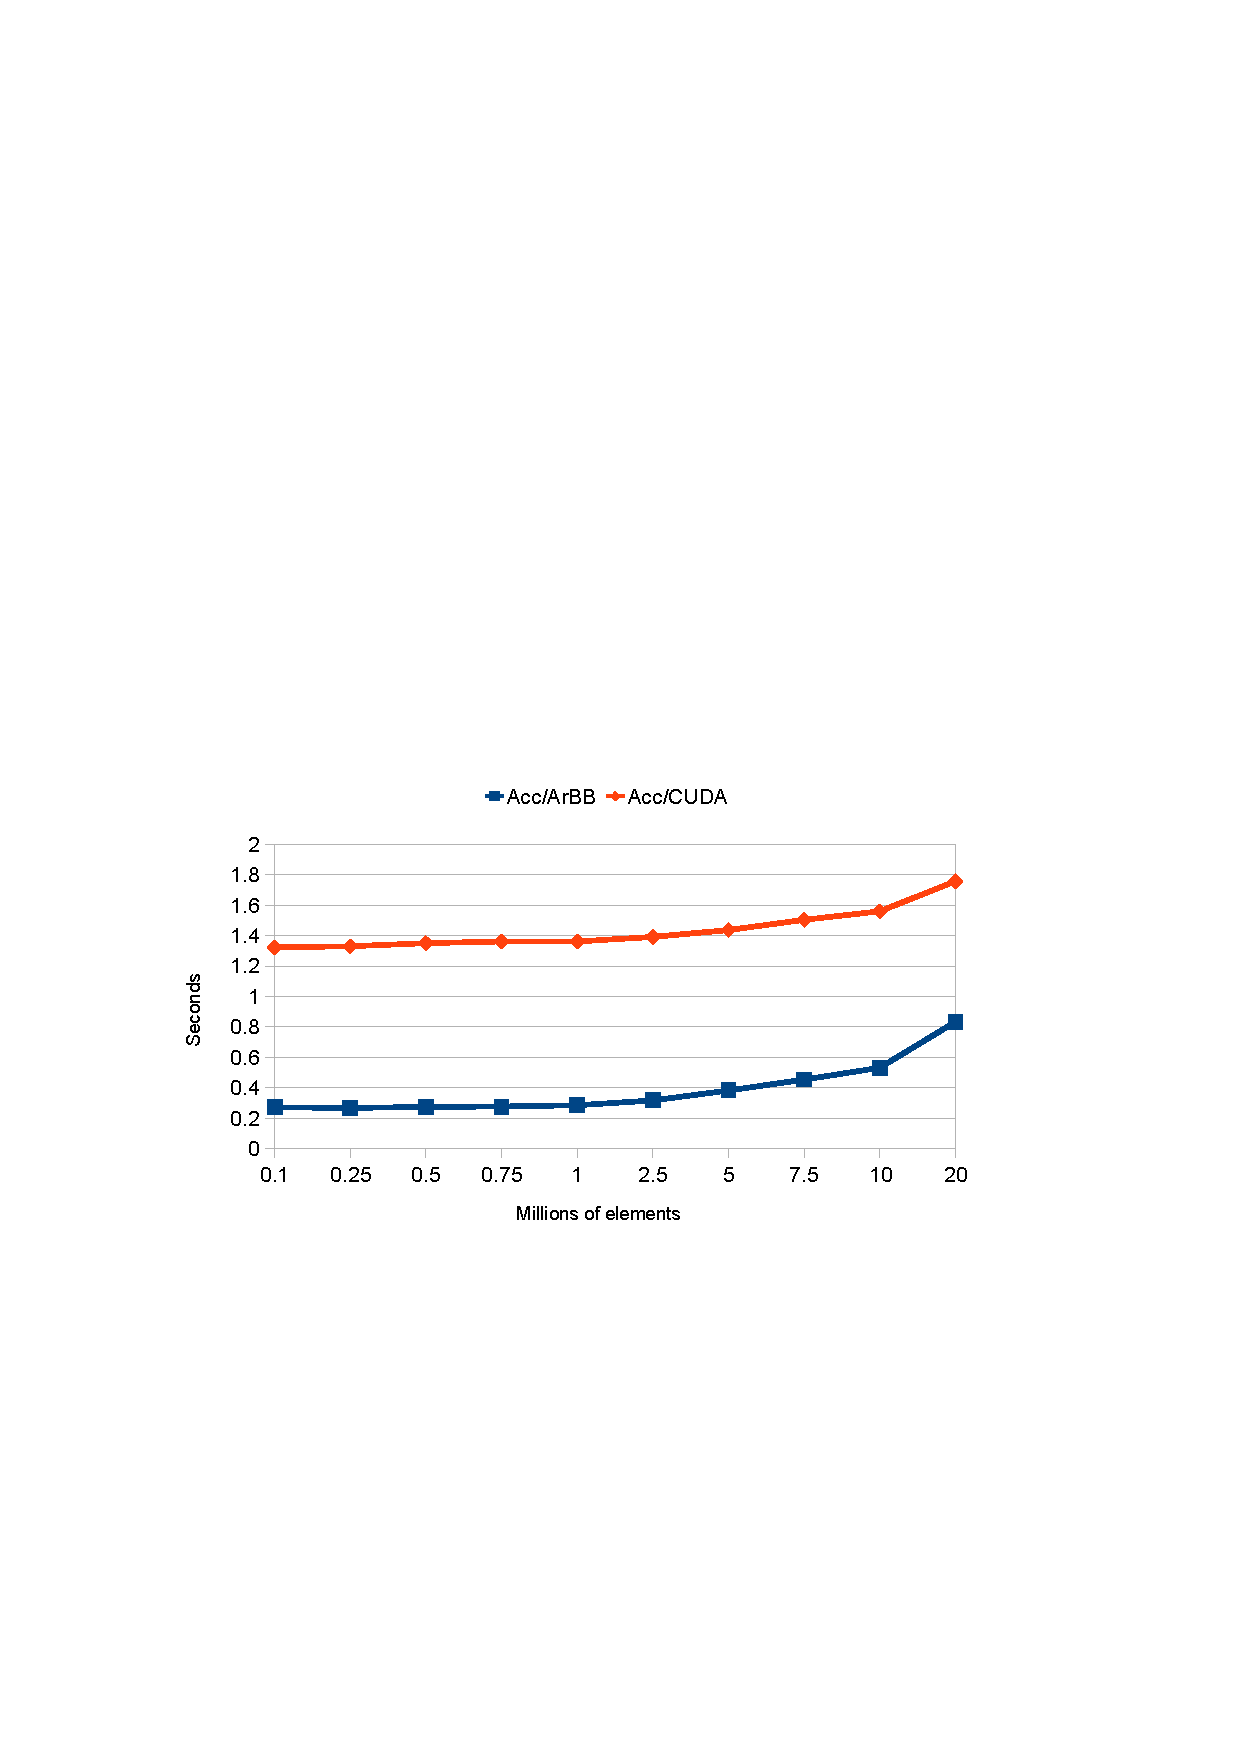
\includegraphics[width=3.5in]{./arbb/jit}    
  \end{center}
\vspace{-5mm}
  \caption{Running time experiments including JIT-time.} 
  \label{f:jit}
\end{figure}

\begin{figure}
  \begin{center}
   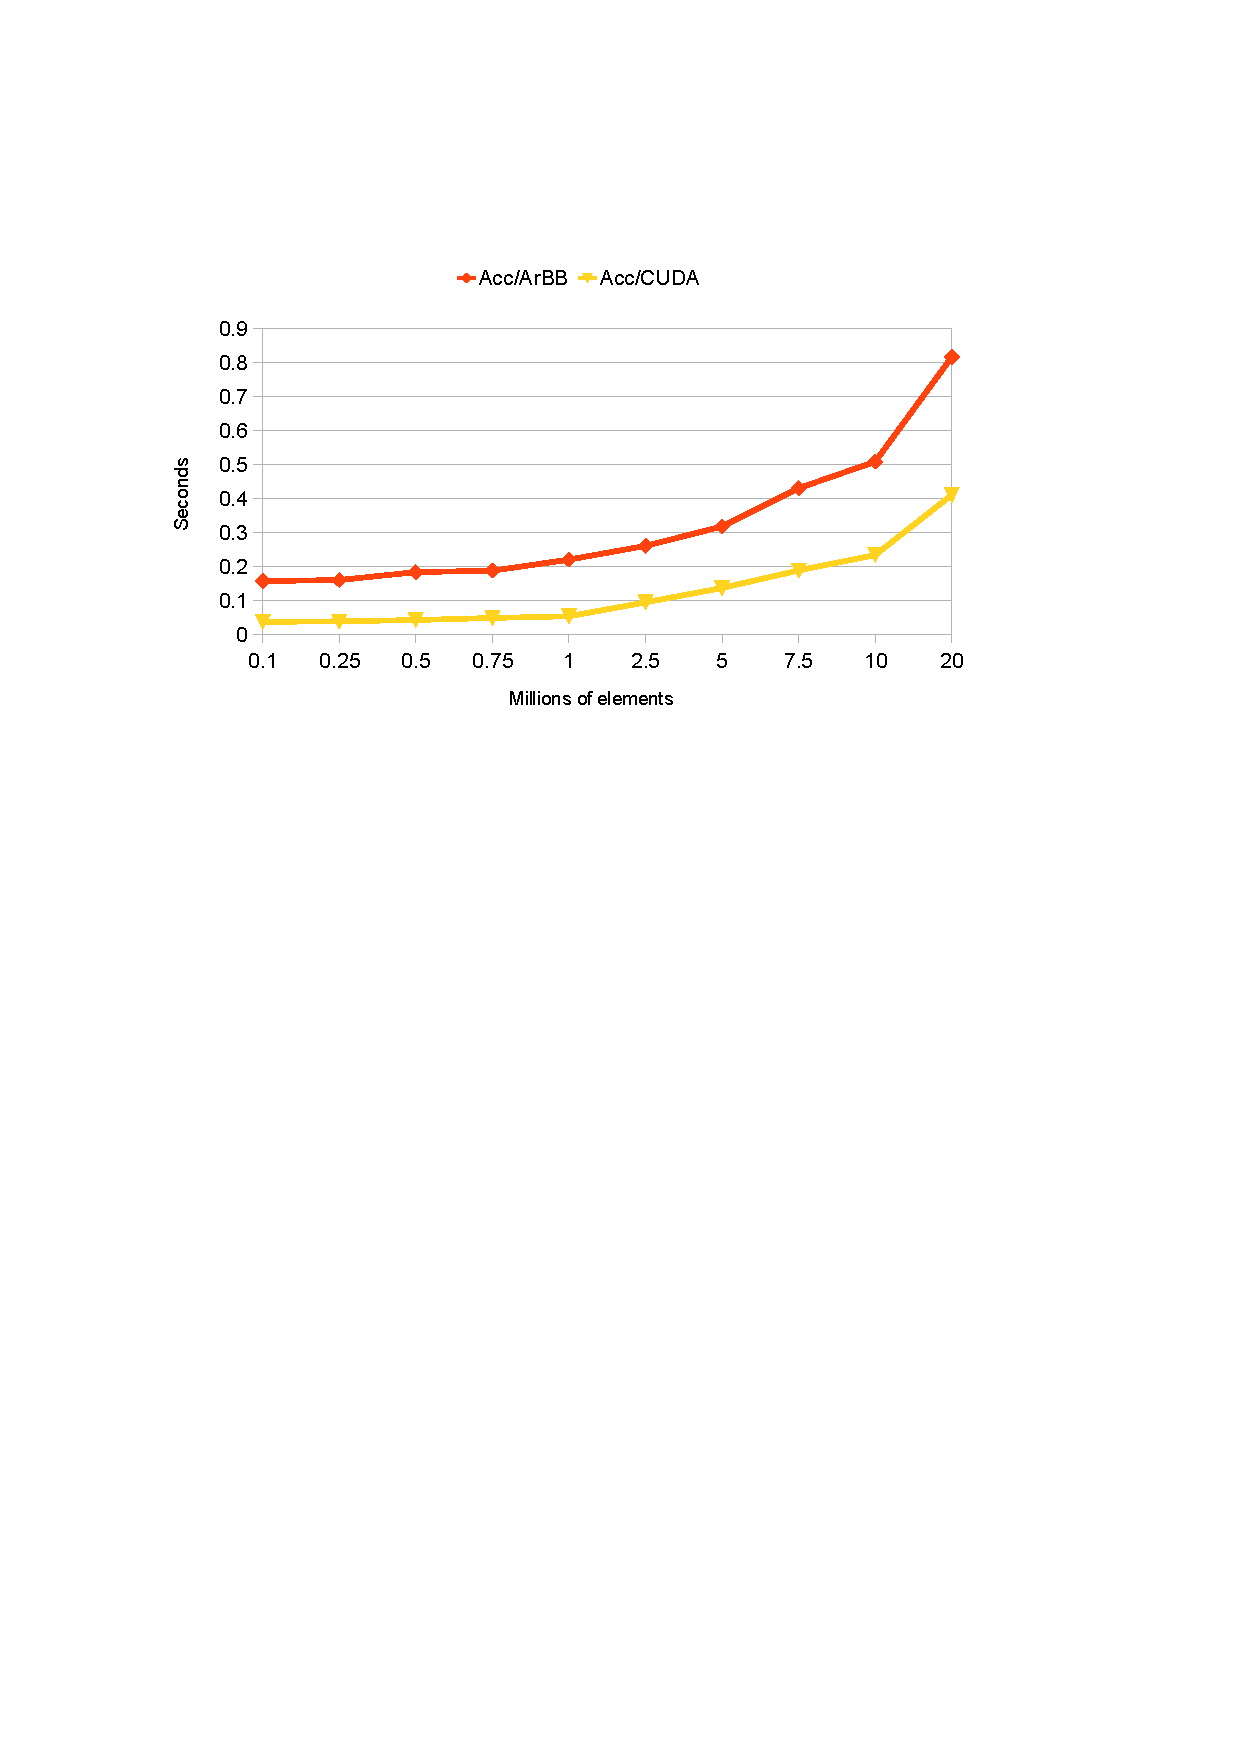
\includegraphics[width=3.5in]{./arbb/nojit}    
  \end{center}
\vspace{-5mm}
  \caption{Running time experiments JIT-time excluded.}
  \label{f:nojit}
\end{figure}


Figures~\ref{f:jit} and \ref{f:nojit} show preliminary results obtained on 
the Black-Scholes benchmark. The figures where obtained on a system with a 4-core 
Intel Core I7 975 machine with HyperThreading. The GPU used was a NVIDIA GTX480.

Figure~\ref{f:jit} shows running times obtained when JIT-time is included. 
% What this figure mainly tells us is that the JITing overhead 
JIT compilation time is much larger 
in the CUDA backend than the ArBB one.  Part of this difference 
can be attributed to the fact that 
the CUDA backend calls an external compiler (\cde{nvcc}), which takes its input in a file and runs in
a separate process.  ArBB, on the other hand, has a library interface to its  JIT-compiler. 
Figure~\ref{f:nojit} shows results obtained when pre-compiling the
CUDA functions eliminating JIT overhead.
In Accelerate, this happens automatically when the same kernel is
invoked repeatedly, because the Accelerate CUDA backed 
uses a caching scheme to avoid unnecessary JIT invocations.  (The
caching functionality has not yet been duplicated in the 
ArBB backend.)

These early results demonstrates the principle that even when a kernel
executes with higher throughput on a GPU, in a particular program it
is difficult to decide whether a computation is worth moving to a GPU,
incurring extra data-movement and possibly extra JIT compilation
\citearbb{wheres-the-data-paper}.  Specifically, we see that the
Accelerate Black-Scholes program from Figure~\ref{fig:blackscholes}
performs better on the CPU if it executes once (even on a large window
of data) whereas the GPU would yield better performance in a sustained
series of executions.
%
Because both CPU and GPU execution may be desirable---and the
selection may be dynamic---it is beneficial to have a single source code
that is portable across both.  
% Accelerate combined with \systemname{} makes this possible.


% ====================================================================================================
\subsection{Related Work}
% ====================================================================================================


OpenCL~\citearbb{opencl08} is a programming model very similar to CUDA but with the aspiration 
to offer both acceleration of computations on GPUs or to multicore CPUs. 
OpenCL JIT compiles the kernels for the particular hardware available and is
in that sense similar to ArBB.  
OpenCL programs are relatively low-level and require a large amount of
boilerplate to create and invoke.  In this sense they occupy a very
different niche than Accelerate.

Microsoft Accelerator~\citearbb{ACCELERATOR} is an embedded language with similar 
aspirations as ArBB, that is, to target a diverse range of architectures using the 
same source code. Accelerate can be used from the C\# language or the 
functional F\# language and targets GPUs or of CPUs and their
vector units.
% However, being part of the .Net framework implies limited accessibility 
%for platforms other than Microsoft Windows.  

\rn{What's the comparison with our stuff?}

%Most work on partitioning workloads between 
Many CPU and GPU comparisons, and some CPU/GPU workload partitioners \citearbb{merge}, rely on
redundant hand-written versions of all kernels
% \citearbb{cpu-gpu-partitioning} 
(though some systems like Qilin \citearbb{qilin} allow a single source code).
It is difficult in this kind of scenario
to make fair comparisons, controlling for the
amount of effort put into the respective implementations.
For example, comparing unoptimized serial CPU implementations vs. GPU
ones is not informative \citearbb{debunking-dubey}.
In \systemname{} controlling for effort
need happen only once---both CUDA and ArBB are
independently optimized by their respective teams of engineers---not for each benchmark.


% ====================================================================================================
% \section{Future work and Conclusions}
%\section{Future Work}
% ====================================================================================================

%\rn{need to be careful about being too repetitive...}
%The \accarbb{} backend is currently work-in-progress. The Accelerate
%functionality is not yet completely covered by the ArBB backend. Currently 
%the ArBB back-ed is operational for Accelerate programs using {\em Map}, 
%{\em ZipWith} and some simple instances of the Accelerate {\em Fold} operation.
%All of these also have the limitation that they only work for up to and 
%including 3-dimensional arrays using the ArBB backend while the Accelerate
%model allows the N-dimensional case. Allowing the N-dimensional case 
%in the ArBB backend for the supported operations range from a simple exercise 
%to more intricate problems needing some thought. For example, in the case 
%{\em Map} operations the needed transformation is simple (Accelerate Maps 
%over N-dimensional arrays is a per-element operation). One could flatten 
%the N-dimensional array to a 1-dimensional array (remembering its old shape) 
%perform the map and then transform the array back into N-dimensions. In 
%the case of {\em Fold} (reductions) the situation becomes more tricky. 
%transforming the arrays to arrays of lesser dimensionality then requires 
%a so-called segmented {\em Fold} operation. 

%The current \accarbb{} backend uses a hybrid of immediate-mode 
%and retained-mode programming styles. Moving more towards 
%retained-mode only may have performance benefits since it would give the 
%ArBB compiler larger programs to optimize. Exploring this aspect is left 
%as future work. 

% ====================================================================================================
\subsection{Discussion and Conclusions}
% ====================================================================================================

We have demonstrated that an EDSL such as Accelerate is sufficiently
platform-independent to break free of its original hardware target
(CUDA/GPU) and create efficient programs on other architectures.  This
gives us hope that \systemname{}/Accelerate programs will be
forward-portable to future parallel architectures and instruction
sets.

The EDSL approach changes the playing field for the designer
of compiler backends.  Rather than contending with full blown
languages and their complexities (e.g. pointers, aliasing,
inheritance, virtual functions, etc), compiler backends can focus on
simple value-oriented compute languages.

%% Achieving the ultimate goal of performance portability requires
%% progress on two research problems.  The first is EDSLs themselves and
%% their integration into host languages.  The second problem 

But the EDSL method solves only part of the performance-portability problem.
Simple as EDSL target languages may be, there remains a
substantial challenge in mapping them efficiently to the diversity
of parallel architectures available now and in the near future.
%especially without requiring a large amount of additional per-platform
%user annotations.
\textred{For example, the idiosyncrasies of memory bank access on
  NVIDIA GPUs must be taken into account to generate efficient
  implementations of the high-level collective operations that we have
  discussed.}

This is a compiler backend research challenge.
The {\em skeletons} method mentioned in
Section~\ref{sec:accelerate-arbb} is one approach to this problem, as
are the optimizations studied in the Copperhead \citearbb{copperhead} and
Obsidian \citearbb{JSLIC} projects.
%
On the other hand, systems that rely on advanced optimizations
typically suffer to some extent from performance-predictability
problems.  Thus achieving portable, predictable performance on a wide range
of architectures---even for the simplest target languages---will
be the subject of much future work.

%{
%\small
\bibliographystylearbb{alpha}
\bibliographyarbb{thesis}
%}


%\end{document}





% ---------------------------------------------------------------------------
% 
% ---------------------------------------------------------------------------
\cleardoublepage 


\section[\paperFTitle]{\paperF: \\ \paperFTitle}
\label{sec:paperF}


%\addcontentsline{toc}{chapter}{Simple and Compositional Reification of Monadic Embedded Languages}

% \paperFTitle

\begin{center} 
Bo Joel Svensson, Mary Sheeran
\end{center}


%\begin{center}
%{\large \bf This paper will be revised before printing the Thesis} 
%\end{center}



%% bare_conf.tex
%% V1.3
%% 2007/01/11
%% by Michael Shell
%% See:
%% http://www.michaelshell.org/
%% for current contact information.
%%
%% This is a skeleton file demonstrating the use of IEEEtran.cls
%% (requires IEEEtran.cls version 1.7 or later) with an IEEE conference paper.
%%
%% Support sites:
%% http://www.michaelshell.org/tex/ieeetran/
%% http://www.ctan.org/tex-archive/macros/latex/contrib/IEEEtran/
%% and
%% http://www.ieee.org/

%\documentclass[conference]{IEEEtran}

%\usepackage{graphicx, color, code}
%\usepackage[cmex10]{amsmath}
%\usepackage{url}
% \usepackage{bookman}  %% bold teletype fonts, but don't know how to prevent it from changing the whole document

% Haven't figured out how to get this to work properly:
%\usepackage[\texttt{cmbtt}]{bold-extra}
% \usepackage{bold-extra} 

%\usepackage{courier}
%\usepackage{fancyvrb}

% correct bad hyphenation here
%\hyphenation{op-tical net-works semi-conduc-tor}


%====================================================================================================
%% FIRST, MISC USEFUL DEFINITIONS
%====================================================================================================

\definecolor{darkgreen}{rgb}{0, 0.5, 0}
\definecolor{darkblue}{rgb}{0,0,0.5}
\definecolor{mygrey}{rgb}{0.7,0.7,0.7}
\newcommand{\textblue}[1]{\textcolor{blue}{#1}}

\newcommand{\cde}[1]{{\footnotesize \tt #1}}

% \newcommand{\kw}[1]{{\bf{#1}}}
\newcommand{\kw}[1]{{\textbf{#1}}}

\newcommand{\comm}[1]{{\em \textcolor{darkgreen}{#1}}}  %% Code comments

\newcommand{\note}[1]{\begin{itemize}\item \textcolor{blue}{#1} \end{itemize}}

%% \newenvironment{mycode}
%% {% This is the begin code
%%   \begin{Verbatim}[commandchars=\\\{\}]}%
%%   %\footnotesize
%%   %\noindent
%%   %\begin{code}\noindent\vspace{-1mm}}
%% %  \begin{code}\noindent}
%% {% This is the end code
%%   \end{Verbatim}
%%   %\end{code} 
%% }

%% \newenvironment{inlinecode}
%% {
%%   \begin{center}
%%   \begin{minipage}{4in}
%%   \begin{mycode}
%% } 
%% {
%%   \end{mycode}
%%   \end{minipage}
%%   \end{center}
%%   \vspace{-1.5ex}
%% }

%% ============================================================
%% USE TO DISABLE COMMENTS:
 \def\noeditingmarks{}
%% ============================================================
\ifx\noeditingmarks\undefined
   \newcommand{\textred}[1]{\textcolor{red}{#1}}
   \newcommand{\pgwrapper}[2]{\textred{#1: #2}}
%   \newcommand{\pgwrapper}[2]{}
   \newcommand{\rnote}[1]{\begin{itemize}\item{\textcolor{blue}{#1}}\end{itemize}}
   \newcommand{\new}[1]{\textcolor{blue}{#1}}
   \newcommand{\const}[1]{\textred{#1}}

%% RRN: Dim the background for Ryan's eyes:
%%   What I need here is a way to do it based on user or host name...
% \pagecolor{mygrey}

\else
   \newcommand{\textred}[1]{#1}
   \newcommand{\pgwrapper}[2]{}
   \newcommand{\rnote}[1]{}
   \newcommand{\new}[1]{#1}
   \newcommand{\const}[1]{#1}
\fi

\newcommand{\js}[1]{\pgwrapper{BJS}{#1}}
\newcommand{\rn}[1]{\pgwrapper{RRN}{#1}}


%% Can we call our ``things'' 
%% ArBB/Haskell for the bindings part ? 
%% Accelerate/ArBB for the Accelerate backend ?
%% This would work with the convention we adopted for 
%%      ArBB/C++  
\newcommand{\systemname}[0]{{Harbb}}
%\newcommand{\systemname}[0]{\textred{HArBB}}

%% This could in theory be separate from the project name..
\newcommand{\accarbb}[0]{\systemname{}}

%% NOTE: THIS SHOULD BE THE SAME AS SYSTEMNAME:
\newcommand{\arbbvmH}[0]{ArBB/Haskell}


%====================================================================================================
% END DEFINITIONS
%====================================================================================================




%\begin{document}
% \title{Painless Portable Vector Parallelism\\ with Haskell and Intel ArBB}
%\title{Programming Future Parallel Architectures\\ with Haskell and Intel ArBB}
% \title{Embedded Domain-Specific Languages Pave the Way for New Parallel Architectures}

%\author{\IEEEauthorblockN{Bo Joel Svensson}
%\IEEEauthorblockA{Dept. of Computer Science and Engineering\\
%Chalmers University of Technology\\
%Gothenburg, Sweden\\
%Email: joels@chalmers.se}
%\and
%\IEEEauthorblockN{Ryan Newton}
%\IEEEauthorblockA{Intel Corporation\\
%Hudson, MA\\
%Email: rrnewton@gmail.com
%}}
% Email: ryan.r.newton@intel.com

%\maketitle

%\begin{abstract}
%
\subsection*{Abstract}
New parallel architectures, such 
\new{as Cell, Intel MIC, GPUs, and tiled architectures, enable} high
performance but are often hard to program.
What is needed is a bridge between high-level programming models 
where programmers are most productive and modern parallel architectures. 
We propose that that bridge is Embedded Domain Specific Languages (EDSLs). 

\new{One attractive target for EDSLs is}
Intel ArBB, a virtual machine for parallel, vectorized computations.
% that serves as a compilation target for EDSLs.
We propose to wed ArBB with the functional programming language
Haskell, {using an EDSL} that generates code for the ArBB VM.  This Haskell integration provides 
% a determinism guarantee 
added safety guarantees compared to other ArBB interfaces.
%
Further, our prototype, \systemname{}, is one of the first EDSL implementations with
optimized backends for multiple parallel architectures (CPU, \new{NVIDIA GPU}, and
others), allowing portability of source code over devices
and their accelerators.


%\end{abstract}
%\IEEEpeerreviewmaketitle




% ====================================================================================================
\subsection{Introduction}
% ====================================================================================================

Are radical new parallel architectures market-feasible if they require
significant changes for programmers?  The jury is out.  In recent
years we have seen difficult-to-program chips suffer 
% \citearbb{cell} 
(e.g. Cell)
and
GPU vendors strive to enable more traditional programming features
\citearbb{fermi} (e.g. C++).  There is an increasing
tension between ease of programming and efficiency.

The tension  shows  across diverse chip markets.  For example,
small embedded devices are most power efficient if their processors and operating systems
omit programming features such as virtual memory and threads \citearbb{tinyos}.  
At the other end of the power spectrum, GPU's
graphics performance may suffer due to inclusion of hardware to ease
GPGPU programming.  In short, there is an opportunity cost to
including extra hardware for programmability.

In this paper, we argue 
that a specific technique holds the greatest promise of solving the programmability dilemma.
%
Domain-specific languages, {\em embedded} within general purpose
languages (EDSLs) 
 enable familiar programming models 
{\em and} flexible
mapping onto new hardware.  The key to having this cake and eating it
too is {\em metaprogramming}.  Familiar programming features are
present, but are eliminated at an intermediate (metaprogram evaluation)
phase and therefore do not reach the parallel hardware itself.


% We present our ongoing work on a
In pursuit of this vision, we offer a
% 
 new EDSL implementation, called \accarbb{}, that combines
existing systems, Accelerate \citearbb{ACCELERATEDAMP11} and ArBB \citearbb{ArBB}, to produce a unified
high-level programming environment equally suited to multicore,
vectorized CPUs, as to GPUs and other accelerators (such as Intel MIC chips \citearbb{larrabee}).
%
\if{0}
ArBB is based on the RapidMind \citearbb{RapidMind} system which was an embedded 
DSL targeting multicore CPUs as well as GPUs. ArBB does not \new{yet} include a GPU 
backend like RapidMind, targeting multicore CPUs and their vector 
units. 
\fi{}
\systemname{} is a single EDSL implementation 
with independently optimized backends \new{by different teams; 
namely, the ArBB backend for CPU/MIC, and a CUDA backend for NVIDIA GPU.}
This makes
\systemname{} an appealing platform for fair CPU/GPU comparisons, 
as well as a compelling programming model for single-source portable performance across a range of
parallel architectures, \new{present and future}.
%%To our knowledge, \systemname{} is the first EDSL implementation with
%%independently optimized backends for CPUs and GPUs.  This makes
%%\systemname{} an appealing platform for fair CPU/GPU comparisons, 
%%as well as a compelling programming
%%model for single-source portable performance across a range of
%%parallel architectures.


% ====================================================================================================
\subsection{Embedded Domain-Specific Languages}
% ====================================================================================================


Domain-specific languages---from Makefiles and \LaTeX{} to
Matlab---are almost too ubiquitous to notice.  Most relevant to our
purposes, domain-specific languages (DSLs) that target a narrow domain and expose communication
patterns to the compiler 
 have achieved performance-portability across a wide range of parallel
architectures.  
StreamIt\citearbb{streamit} is a good example.
% (for example, StreamIt\citearbb{streamit})
% The high-water mark in this area is perhaps  StreamIt\citearbb{streamit}.
% 

% It has been noted \citearbb{not-sure} that 
% Yet the few DSLs that gain popularity lose simplicity\citearbb{not-sure}.  
% Yet popular DSLs rarely remain simple \citearbb{not-sure}.  
DSLs may start out simple and focused, but if they gain popularity
they quickly grow in complexity to rival full-blown languages.
Feature creep
can make DSL implementations complex and expensive to maintain.
Further, non-standard DSL syntax and features present a learning curve for users.  In the
last ten years an attractive solution to this dilemma has emerged: {\em
  embed} each DSL into a general-purpose host language that can provide
common functionality with familiar syntax and semantics.
% in place of the DSL.

When embedding, host language programs {generate} DSL programs;
% Embedding means that the host language is used to generate DSL programs; 
the {\em deeper} the embedding, the more integrated the
DSL into the syntax and type-system of the host language.
%
% Typically, %% pruning weasel words
A key host-language feature for embedding is that
language constructs can be overloaded to operate over {\em abstract
  syntax trees} (ASTs)\footnote{This ad-hoc polymorphism is accomplished,
for example, through operator-overloading in C++ or type classes in
Haskell.}.  For example, the following simple function operates on scalars:


\vspace{1mm}
\begin{Verbatim}[commandchars=\\\{\}]
  float f(float x) \{ return (2*x - 1); \}
\end{Verbatim}
\noindent
But simply by changing the types, \cde{f} might be lifted to operate on {\em
  expressions} (which, when evaluated, will yield \cde{floats}):

\vspace{1mm}
\begin{Verbatim}[commandchars=\\\{\}]
  \kw{exp<float>} f(\kw{exp<float>} x) \{
    return (2*x - 1);
  \}
\end{Verbatim}

A common arrangement is for the host language program to execute at
runtime but to generate ASTs that are executed by a just-in-time
(DSL) compiler.  This use of metaprogramming (program generation)
differs from the more common usage of preprocessors and 
% Lisp/Scheme macros \citearbb{scheme-macros}
macros, which typically add extra
phases of computation {\em before}  compile time---increasing
the number of compile-time rather than runtime phases.

% EDSLs typically add additional runtime phases.  That is, the host language program 
% executes at runtime but uses a JIT to process generated ASTs.
%% which are
%% usually used to perform computation {\em earlier} than the usual
%% compile time, embedded DSLs (EDSLs) typically defer computation 


One reason that EDSLs are good for productivity is that the programmer
gains the software engineering benefits of the host language
(object-orientation, higher-order-functions, modules, etc), while not
paying the cost at runtime for additional layers of abstraction or
indirection.  Indeed, the embedded languages for 
performance-oriented EDSLs are often simple, first-order
languages without pointers \citearbb{wavescript, ACCELERATEDAMP11}.

% , paul-lius-thingy

% regiment,
As a research area, EDSLs and two-stage DSLs have been actively pursued for at least a
decade \citearbb{VERTIGO, wavescript} but are gaining steam
recently 
%\citearbb{sejits, stanford-ppl} 
\citearbb{copperhead, stanford-ppl} 
and are beginning to appear in
commercial products \citearbb{ArBB}.
%
Further, EDSL techniques have spread beyond their origin in 
 the programming languages community.
% 
For example, both Stanford's Parallel Programming Laboratory (PPL) and
the Berkeley Parlab are creating EDSLs as their flagship parallel
programming solutions for domains such as machine learning and
rendering \citearbb{stanford-ppl}.
  Moreover, EDSLs need not be hosted by esoteric research languages---Intel's
 ArBB embeds an array language in C++ and Berkeley's
Copperhead \citearbb{copperhead} generates CUDA from simple Python code.

%\rnote{Is there a good motivating example program?  What are some of
%  the Metaocaml motivating examples?}

{For the remainder of this paper we will focus our discussion
  on the Intel ArBB VM, a virtual machine for just-in-time
  generation of vector codes, \new{which implements a restricted} domain-specific
  language of array computations.  In this paper we introduce
  {\em High-level ArBB}, 
  (\systemname{}), an EDSL that internally uses the ArBB
  VM.  \new{While Intel's ArBB package already includes an EDSL targeting the VM (for C++)},
\systemname{} \new{offers additional advantages, including}
  more succinct programs and additionally safety
  guarantees---namely, complete deterministic-by-construction parallel
  programs (across both host and VM languages).}


% ====================================================================================================
% \section{Accelerate and ArBB}
%\section{\accarbb{}:  ArBB and Accelerate}
\subsection{\accarbb{} $=$ ArBB $+$ Accelerate}
\label{sec:accelerate-arbb}
% ====================================================================================================

Our first \systemname{} prototype adapts an existing EDSL called {\em
  Accelerate} (Data.Array.Accelerate).  Accelerate targets high-level
data-parallel programming in Haskell.
Previous work on Accelerate has focused on developing a CUDA-backend
for GPU programming.  In this paper we describe our effort to retarget
Accelerate to ArBB.  

With respect to determinism guarantees, the existing Intel ArBB product
represents an integration of the safe (ArBB VM) with the unsafe (C++).
In the Haskell context, because purely functional computations are
guaranteed deterministic (even when executed in parallel), and because
ArBB computations invoked by Haskell functions are themselves free of
side-effects, \systemname{} achieves a
guarantee of determinism for complete programs that combine both
Haskell computation and ArBB VM computation.
% which offers portability.
% (The 'H' in \systemname{} therefore stands for Haskell as well as ``High-level''.)


%% {\em Accelerate} (Data.Array.Accelerate) is an existing EDSL for 
%% high-level data-parallel programming in Haskell~\citearbb{Accelerate}. 
The Accelerate programming model consists of collective 
operations that can be performed over arrays, together with a simple 
language of scalar expressions\new{---in the current release, the Haskell type system enforces that parallelism not be nested.}
\if{0}
The Haskell type 
system is used to enforce that no nested data-parallelism can be expressed 
\new{(in the current release, this may be relaxed in the future).}
\fi{}
Accelerate's collective operations include {\em Map} (akin to parallel
for loops) {\em ZipWith} (a generalization of elementwise vector addition) and 
{\em Fold} (sum generalized)---familiar operations for programmers versed in the functional paradigm.
All of these collective operations are easily parallelizable. 
% In the case of {\em Map} and {\em ZipWith} the potential for parallelism is abundant.  

%% dotProd :: Vector Float -> 
%%            Vector Float -> 
%%            Acc (Scalar Float) 
\begin{Verbatim}[commandchars=\\\{\}]
dotProd (xs :: Vector Float) 
        (ys :: Vector Float) = 
  \kw{let} xs\_ = use xs 
      ys\_ = use ys 
  \kw{in}  fold (+) 0 (zipWith (*) xs\_ ys\_) 
\end{Verbatim}

The Accelerate code listing above specifies a function that takes two 1-dimensional 
arrays as inputs (of type \cde{Vector Float}, e.g. a vector of floats). The result of the function is a single
scalar. 
% (\cde{Scalar Float})
The \cde{use} function is applied to an array to convert it 
for use in the collective operations provided by Accelerate;
\cde{use} 
% is actually a function with type \cde{Vector a -> Acc (Vector a)} and 
may result in
copying the array to, for example, the GPU in the case of Accelerate's 
CUDA backend.  

After applying \cde{use} to bring in input data, the programmer then
constructs a data-parallel program from collective operations.
Above, \cde{fold} is a function that takes three arguments, 
here those arguments are \cde{(+)},  $0$ and \cde{zipWith (*) xs\_ ys\_}. 
\cde{zipWith}, in turn, is a function taking three arguments, \cde{(*)}, 
\cde{xs\_} and \cde{ys\_}. The \cde{zipWith} operation here applies pairwise 
multiplication to the two arrays and the \cde{fold} sums up all the elements 
into a single scalar. 

%\rn{Following para slightly redundant but ok...}
%Accelerate makes GPU programming accessible to the functional programmer 
%by offering a familiar set of operations. This set of operations also have 
%the beneficial property that they have inherent parallelism and are 
%easily implementable on the GPU. 

Accelerate's CUDA backend implements collective operations using
a hand-tuned ``skeleton'' for each operation (and possibly for
different hardware versions). The kernel---for example, the function
to mapped over the dataset---is 
instantiated into the body of the skeleton code. The resulting 
program is compiled using the NVIDIA CUDA compiler and dynamically linked 
into the running Haskell program.

%\subsection{Intel Array Building Blocks (ArBB)}
\subsection{Intel Array Building Blocks (ArBB)}
\label{sec:arbb}

%ArBB is embedded in the C++ programming language but it also exposes a 
%very low level API that is purely C. 
%{\em ArBB} (Array Building Blocks) is also an embedded DSL. 
The operations exposed by ArBB are similar to those of Accelerate. 
In ArBB, parallel computations are expressed using a set of built-in 
primitives. All vectorization and threading is managed internally by 
ArBB. The programmer uses collective operations with a clear semantics 
such as \cde {add\_reduce} that computes the sum of the elements in a given 
array. ArBB also has language constructions for control flow, conditionals
and loops. These operations have their usual sequential semantics and are not 
parallelized by the system, rather, only specific collective operations are executed
in parallel. 

Today's existing ArBB product is embedded in C++ and provides special
types for scalars and arrays (e.g. \cde{dense<f32>} rather than \cde{vector<float>}).
Using ArBB/C++ to express the dot product computation can be done 
as follows:

%\vspace{2mm}
\begin{Verbatim}[commandchars=\\\{\}]
\kw{void} dot\_product(\kw{const} dense<f32>& a, 
                 \kw{const} dense<f32>& b,
                 f32& c) 
{ 
  c = add\_reduce(a * b);
}
\end{Verbatim} 


% The above program takes two arrays of type \cde{dense<f32>} as input. 
% \cde{dense<f32>} specifies a 1-dimensional array of 32-bit floating
% point values. The result is a single 32-bit float.  

Note that arithmetic operators such as (*) are overloaded 
for to operate on arrays as well as scalars (e.g. \cde{a * b} above).
Thus, the above C++ function multiplies two arrays before summing them with \cde {add\_reduce}:

The code listing below is indicative to the amount of glue code needed to invoke an 
ArBB computation\footnote{In OpenCL and CUDA the glue code situation is even worse}. It shows how the dot product code is launched using {\tt call} and 
how data is bound, {\tt bind}, for use in ArBB. 

\vspace{2mm}
\begin{Verbatim}[commandchars=\\\{\}]
\kw{int} main() 
\{ 
  double a[SIZE];
  double b[SIZE];

  for ( \kw{int} i = 0; i < SIZE; ++i) \{ 
    a[i] = ...; b[i] = ...;
  \}
  dense<f32> va, vb;
  f32 vc;
  bind(va, a, SIZE); 
  bind(vb, b, SIZE); 
  call(dot\_product)(va, vb, &vc); 
  ...
\}
\end{Verbatim}


%\rnote{SPECIFICALLY ADDRESS THE FUNCTIONALITY GAP?  E.G general
%  reduce.  Any other examples?}

The model provided by Accelerate is slightly richer than that of ArBB.
Even the two very simple \cde {dot\_product} examples above manage to illustrate 
this. In Accelerate there is a more general reduction primitive called \cde {fold} 
where in ArBB there are specific reductions, \cde {add\_reduce}, \cde {mul\_reduce} 
and so on. Not visible in these small examples is another difference, Accelerate 
operations are generalized to arbitrary dimensions while ArBB operations are 
limited to 1, 2, and 3 dimensions (and 0, i.e. scalar). These differences aside,
the ArBB and Accelerate programming models are very similar.


% ====================================================================================================
\subsection{Implementation of \systemname{}} 
% ====================================================================================================


%\rnote{Sadly the Haskell details don't buy us much here... what are
%  the {\em conceptual} problems solved in mapping the Accelerate
%  abstraction to the ArBB one?  The data models are similar, but
%  there are always mismatches -- dimensionality support, missing
%  reduction.}

%\rnote{What is the technique that you are using to address these sorts
%  of problems?  Is there anything to say about it?}

\begin{figure}
  \begin{center}
   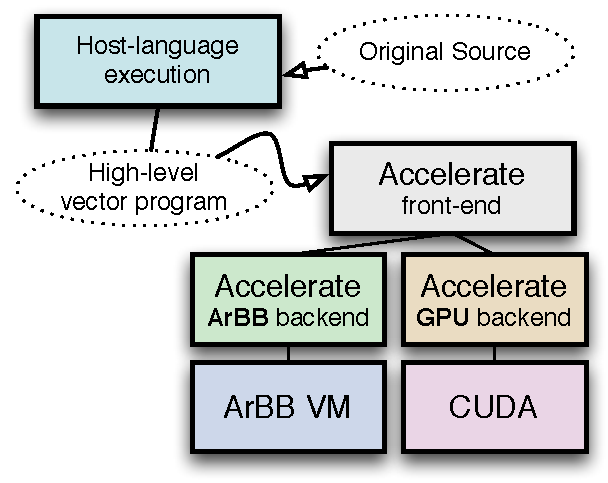
\includegraphics[width=2.0in]{./arbb/figure_architecture}    
  \end{center}
\vspace{-5mm}
  \caption{Architecture of the \systemname{} system.  \rn{(ROUGH.)}}
  \label{f:architecture}
\end{figure}


Using Accelerate and ArBB together, we propose a layered architecture
for \systemname{},
% Our goal is to make the benefits of ArBB available to the Haskell programmer. 
% \js{(Or is our goal to give an even better ``front-end'' to ArBB compared to C++)}
% We propose that this is best accomplished using a layered approach, as
pictured in Figure~\ref{f:architecture}. 
The host language execution (via Haskell in this case) executes the
programmer's source code, generating a vector program in the
restricted language of the Accelerate front-end.
Then either Accelerate backend---ArBB or CUDA---may be used.
The 
bottom layer of the ArBB backend consists of a direct mapping of the ArBB virtual machine
API (VMAPI) into Haskell including one-to-one bindings for each C 
function. 
To [partially] automate the creation of these bindings we used the C2HS system \citearbb{C2HS}. The 
\arbbvmH{} bindings are very low-level.
%and make little use of the high-level programming methods that
% Haskell programmers want. 
The idea 
is that the \arbbvmH{} bindings should be used to implement
backends for higher-level data-parallel EDSLs.

%% To illustrate our position we 
%% have started working on a backend to the successful DSL Accelerate 
%% (Data.Array.Accelerate) using our \arbbvmH{} bindings. 

To address the functionality mismatch between Accelerate and ArBB,
when possible we reencode the users Accelerate program using existing
ArBB mechanisms.  Our prototype does not support 100\% of Accelerate's
compute model (for example, only supporting  up to three-dimensional
arrays), but the remaining functionality can be mapped onto ArBB in
time using known methods---for example, our compiler could map higher
dimensional arrays onto a specific lower-dimensional data-layout.

%% The programming models supported by ArBB and Accelerate are very similar. 
%% Both obtain their parallelism by exposing collective operations 
%% such as {\em Map}, {\em Reduce}, {\em ZipWith} and {\em Scan} (all prefixes operations). However, 
%% the functionality match is not 100\%. For example, Accelerate supports {\em Map} operations 
%% over N-dimensional Arrays while ArBB supports them only up to 3-dimensions. 
%% Similar inconsistencies apply to the other operations as well. \textred{The current
%% ArBB backend simply disallows Accelerate programs using too high dimensionality
%% of the arrays.} \rn{Sure, we want to say that we're not done closing
%%   this gap (for
%%   accuracy) but more importantly we want to identify whether
%%   techniques exist to close the gap.  Presumably, yes?  We can
%%   ourselves collapse the dimensionality of arrays before giving them
%%   to ArBB?  Are there any operations that would defeat that technique?}
%

One example of a functionality discrepancy bridged by our
implementation is reductions.  As mentioned in \ref{sec:arbb},
Accelerate allows the programmer to reduce using an arbitrary
associative function, but ArBB has only built-in reductions with fixed
operations (add, multiply, xor, etc). We plan to provide general reductions in
the ArBB backend by a two-fold strategy:

\begin{enumerate}
\item Attempt to map an Accelerate reduction directly onto an ArBB
  primitive such as \cde{add\_reduce}.
\item Apply a general reduction technique based on $log(N)$ map
  operations over successively halving array sizes.  Essentially, cut
  the array in half, combine the halves, repeat. In ~\citearbb{reduction}
  this approach is explained in the context of CUDA. 
\end{enumerate}

%% \rn{Is the technique worthy of
%%   description?  Can we just cite the CUDA documentation or something
%%   since it's common?} 

In our current experiments, approach (2) is significantly slower.
Therefore, the ideal would be that ArBB exposed general reduction
directly in its programming model.  We expect this functionality to be
added in future releases.  In the meantime we plan to explore a
technique that would allow us to maximize the number of situations in
which (1) above applies.  Namely, a reduce operation can often be {\em
  factored} into a map followed by a reduce.  For example, a reduction
that multiplies each input number by a coefficient and sums the
results can be split into a map phase for the multiplication followed
by the built-in \cde {add\_reduce} operator.

%% Currently, our reduction implementations in ArBB 
%% are many times 
%% slower (\textasciitilde 20x) than their built-in counterparts. 
%% % To ameliorate this present performance problem we attempt to map
%% % programmers 
%% Our present workaround for this performance problem is to let 
%% \accarbb{} inspect the reduction function and switch to efficient 
%% built in  ArBB reduction where possible.  
%% \rn{Future work may be to decompose reductions into map+reduce so as
%%   to allow the reduce to become a builtin.}


Another choice faced by our implementation is the granularity at which the
ArBB JIT is invoked.  Specifically, should each collective operation result in its
own call to the ArBB JIT (in ArBB terminology, {\em
  immediate-mode}, akin to the pre-OpenGL 3.0 immediate mode), or
should multiple collective operations be placed together
inside an ArBB function and passed to the JIT?
We will call the latter approach {\em retained-mode}.

%% In immediate-mode the 
%% operations called from the ArBB API are executed
%% synchronously---before each API call returns. In retained-mode, ArBB
%% collects calls and, only when results are requested, the 
%% entire computation is optimized 
%% and executed. 

Retained-mode generally offers performance benefits; a bigger 
chunk is given to the JIT compiler, enabling cross-optimization
between collective operations. 
Our prototype Accelerate backend uses 
ArBB in  
a combination of immediate- and retained-mode. The main collective 
operations are compiled using the retained-mode. For example, in the case 
of a \cde{map f}  operation first the function to be mapped is created and 
compiled using retained-mode then a small {\em mapper} function is 
also created and compiled using retained-mode. 
%% The mapper function is 
%% of course very small and therefore does not give much to the JIT compiler 
%% to work on optimization-wise. 
Between the collective operations the backend
needs to perform data management and copying, which 
are performed in immediate-mode. It is our belief that 
\systemname{} would benefit from using retained-mode exclusively 
but we leave that as future work. 





% ====================================================================================================
\subsection{Preliminary Results}
% ====================================================================================================

%\rnote{One tiny benchmark if we can manage it.}

%\rnote{Ideally: Something like blackscholes running Arbb/C++,
%  \systemname{}, CPU+GPU, possibly compared to other blackscholes
%  implementations -- say Cilk on CPU and hand-coded CUDA (I can
%  provide the former I think).  Perhaps serial, non-vectorized CPU for
%  comparison.}

%\rnote{Point 1 -- High level thing is within X\% of low level thing.
%  The usual.  But we also want to say that \systemname{} is no worse
%  than ArBB/C++ -- the metalanguage doesn't matter, be it Haskell,
%  Python, or C++.}

%\rnote{Point 2 -- It's important to do a good job on the CPU side.
%  Even if you don't beat GPU there's a big difference between
%  vectorizing/not-vectorizing (and using multicore of coarse).  Can't
%  be ignored.}

%\rnote{Bonus points -- if we could show how bad ``naive'' ports are that
%  would be nice.  How well does your C CPU code run on GPU unmodified
%  (or minimally ported)?}



%\rnote{CPU/GPU systems that do a good job of both.  Perhaps quickly
%  dismiss those that make no effort on the CPU side.}

Black-Scholes option pricing is a finance-related benchmark that has been used in similar
DSLs targeting GPUs \citearbb{ACCELERATEDAMP11, NIKOLA}. Since we are re-using the 
Accelerate front-end, we can directly use the Black-Scholes benchmark that 
is shipped with that system.  Figure \ref{fig:blackscholes} shows the
complete code listing for an Accelerate Black-Scholes function which
can be executed on GPUs or any processor targeted by ArBB.

% blackscholes :: Vector (Float, Float, Float) 
%
%                -> Acc (Vector (Float, Float))
%\fbox{

%       r     = \textit{constant} riskfree
%       v     = \textit{constant} volatility

\begin{figure}
\begin{footnotesize}
\begin{Verbatim}[frame=single, commandchars=\\\{\}]
blackscholes (xs :: Vector (Float,Float,Float)) = 
  map kernel (\textit{use} xs)

kernel x =
  \kw{let} (price, strike, years) = \textit{unlift} x
      r     = 0.02 \textsf{\textit{-- riskfree constant}}
      v     = 0.30 \textsf{\textit{-- volatility constant}}
      sqrtT = sqrt years
      d1    = (log (price / strike) + 
                   (r + 0.5 * v * v) * years) / 
              (v * sqrtT)
      d2    = d1 - v * sqrtT
      cnd d = d >* 0 ? (1.0 - cndfn d, cndfn d)
      cndD1 = cnd d1
      cndD2 = cnd d2
      expRT = exp (-r * years)
  \kw{in} \textit{lift} ( price * cndD1 - 
            strike * expRT * cndD2
          , strike * expRT * (1.0 - cndD2) - 
            price * (1.0 - cndD1))

cndfn d =
  \kw{let} poly  = horner coeff
      coeff = [0, 0.31, -0.35, 1.78, -1.82, 1.33]
      rsqrt = 0.39894228040143267793994
      k     = 1.0 / (1.0 + 0.2316419 * abs d)
  \kw{in} rsqrt * exp (-0.5*d*d) * poly k

horner coeff x = 
  \kw{let} madd a b = b*x + a
  \kw{in}  foldr1 madd coeff
\end{Verbatim}
\end{footnotesize}
\caption{Complete code listing for a Black-Scholes function expressed
  in Haskell syntax using the Accelerate and \systemname{} libraries.
  Invocations of the functions \cde{use}, \cde{lift} and \cde{unlift}
%  and \cde{constant} 
represent additional boilerplate added for
  conversion in and out of Accelerate types.  Specifically, \cde{lift} and
  \cde{unlift} convert tuples and handle the fact that Accelerate
  arrays of tuples are really implemented as tuples of arrays.
  Otherwise, the program is identical to a plain Haskell
  implementation.}
\label{fig:blackscholes}
\end{figure}


%% \end{code}
%%  %605993438
%% % horner :: Num a => [a] -> a -> a
%% \begin{code}
%% \footnotesize



The kernel of this algorithm performs arithmetic on triples of
floating point numbers, creating pairs of floats as results. The problem 
is embarrassingly parallel, consisting of independent computations
for every element of an array (a map).

\begin{figure}
  \begin{center}
   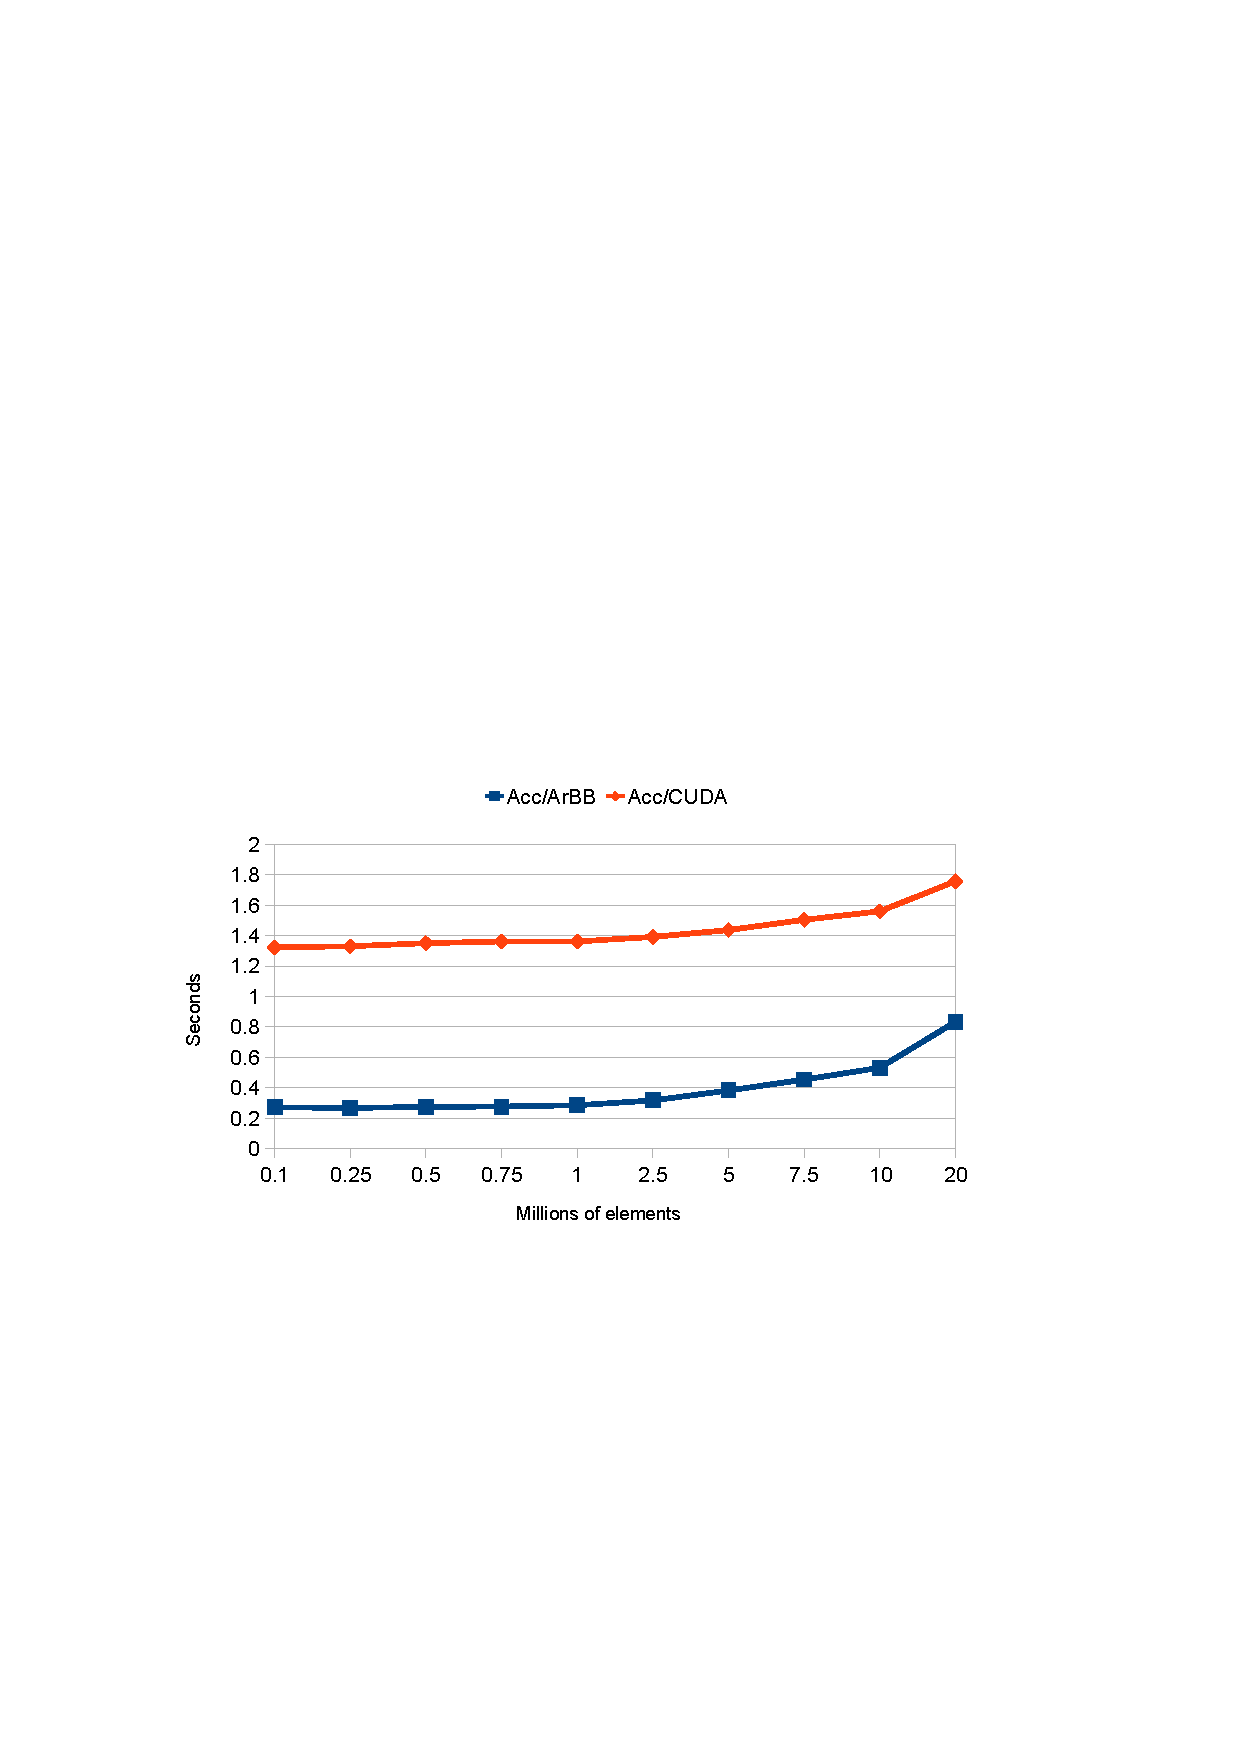
\includegraphics[width=3.5in]{./arbb/jit}    
  \end{center}
\vspace{-5mm}
  \caption{Running time experiments including JIT-time.} 
  \label{f:jit}
\end{figure}

\begin{figure}
  \begin{center}
   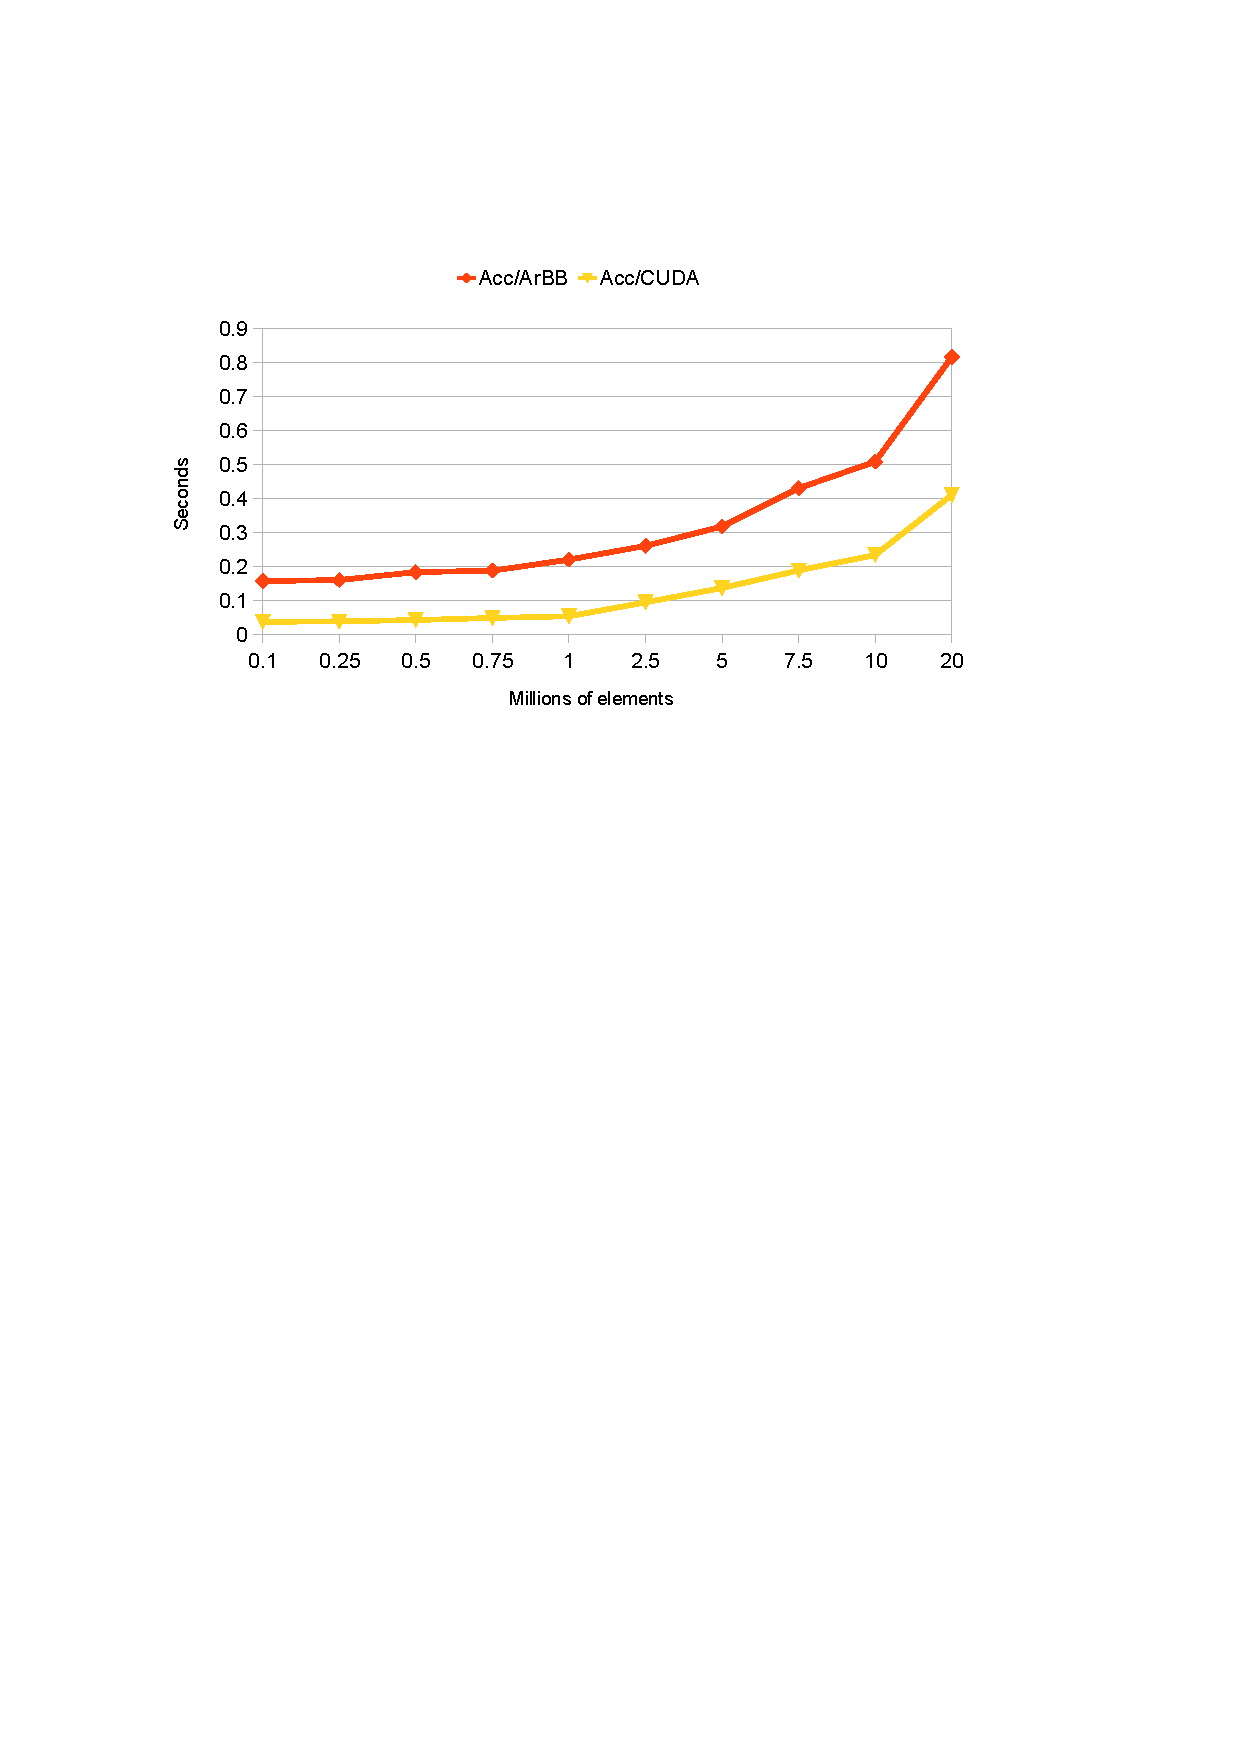
\includegraphics[width=3.5in]{./arbb/nojit}    
  \end{center}
\vspace{-5mm}
  \caption{Running time experiments JIT-time excluded.}
  \label{f:nojit}
\end{figure}


Figures~\ref{f:jit} and \ref{f:nojit} show preliminary results obtained on 
the Black-Scholes benchmark. The figures where obtained on a system with a 4-core 
Intel Core I7 975 machine with HyperThreading. The GPU used was a NVIDIA GTX480.

Figure~\ref{f:jit} shows running times obtained when JIT-time is included. 
% What this figure mainly tells us is that the JITing overhead 
JIT compilation time is much larger 
in the CUDA backend than the ArBB one.  Part of this difference 
can be attributed to the fact that 
the CUDA backend calls an external compiler (\cde{nvcc}), which takes its input in a file and runs in
a separate process.  ArBB, on the other hand, has a library interface to its  JIT-compiler. 
Figure~\ref{f:nojit} shows results obtained when pre-compiling the
CUDA functions eliminating JIT overhead.
In Accelerate, this happens automatically when the same kernel is
invoked repeatedly, because the Accelerate CUDA backed 
uses a caching scheme to avoid unnecessary JIT invocations.  (The
caching functionality has not yet been duplicated in the 
ArBB backend.)

These early results demonstrates the principle that even when a kernel
executes with higher throughput on a GPU, in a particular program it
is difficult to decide whether a computation is worth moving to a GPU,
incurring extra data-movement and possibly extra JIT compilation
\citearbb{wheres-the-data-paper}.  Specifically, we see that the
Accelerate Black-Scholes program from Figure~\ref{fig:blackscholes}
performs better on the CPU if it executes once (even on a large window
of data) whereas the GPU would yield better performance in a sustained
series of executions.
%
Because both CPU and GPU execution may be desirable---and the
selection may be dynamic---it is beneficial to have a single source code
that is portable across both.  
% Accelerate combined with \systemname{} makes this possible.


% ====================================================================================================
\subsection{Related Work}
% ====================================================================================================


OpenCL~\citearbb{opencl08} is a programming model very similar to CUDA but with the aspiration 
to offer both acceleration of computations on GPUs or to multicore CPUs. 
OpenCL JIT compiles the kernels for the particular hardware available and is
in that sense similar to ArBB.  
OpenCL programs are relatively low-level and require a large amount of
boilerplate to create and invoke.  In this sense they occupy a very
different niche than Accelerate.

Microsoft Accelerator~\citearbb{ACCELERATOR} is an embedded language with similar 
aspirations as ArBB, that is, to target a diverse range of architectures using the 
same source code. Accelerate can be used from the C\# language or the 
functional F\# language and targets GPUs or of CPUs and their
vector units.
% However, being part of the .Net framework implies limited accessibility 
%for platforms other than Microsoft Windows.  

\rn{What's the comparison with our stuff?}

%Most work on partitioning workloads between 
Many CPU and GPU comparisons, and some CPU/GPU workload partitioners \citearbb{merge}, rely on
redundant hand-written versions of all kernels
% \citearbb{cpu-gpu-partitioning} 
(though some systems like Qilin \citearbb{qilin} allow a single source code).
It is difficult in this kind of scenario
to make fair comparisons, controlling for the
amount of effort put into the respective implementations.
For example, comparing unoptimized serial CPU implementations vs. GPU
ones is not informative \citearbb{debunking-dubey}.
In \systemname{} controlling for effort
need happen only once---both CUDA and ArBB are
independently optimized by their respective teams of engineers---not for each benchmark.


% ====================================================================================================
% \section{Future work and Conclusions}
%\section{Future Work}
% ====================================================================================================

%\rn{need to be careful about being too repetitive...}
%The \accarbb{} backend is currently work-in-progress. The Accelerate
%functionality is not yet completely covered by the ArBB backend. Currently 
%the ArBB back-ed is operational for Accelerate programs using {\em Map}, 
%{\em ZipWith} and some simple instances of the Accelerate {\em Fold} operation.
%All of these also have the limitation that they only work for up to and 
%including 3-dimensional arrays using the ArBB backend while the Accelerate
%model allows the N-dimensional case. Allowing the N-dimensional case 
%in the ArBB backend for the supported operations range from a simple exercise 
%to more intricate problems needing some thought. For example, in the case 
%{\em Map} operations the needed transformation is simple (Accelerate Maps 
%over N-dimensional arrays is a per-element operation). One could flatten 
%the N-dimensional array to a 1-dimensional array (remembering its old shape) 
%perform the map and then transform the array back into N-dimensions. In 
%the case of {\em Fold} (reductions) the situation becomes more tricky. 
%transforming the arrays to arrays of lesser dimensionality then requires 
%a so-called segmented {\em Fold} operation. 

%The current \accarbb{} backend uses a hybrid of immediate-mode 
%and retained-mode programming styles. Moving more towards 
%retained-mode only may have performance benefits since it would give the 
%ArBB compiler larger programs to optimize. Exploring this aspect is left 
%as future work. 

% ====================================================================================================
\subsection{Discussion and Conclusions}
% ====================================================================================================

We have demonstrated that an EDSL such as Accelerate is sufficiently
platform-independent to break free of its original hardware target
(CUDA/GPU) and create efficient programs on other architectures.  This
gives us hope that \systemname{}/Accelerate programs will be
forward-portable to future parallel architectures and instruction
sets.

The EDSL approach changes the playing field for the designer
of compiler backends.  Rather than contending with full blown
languages and their complexities (e.g. pointers, aliasing,
inheritance, virtual functions, etc), compiler backends can focus on
simple value-oriented compute languages.

%% Achieving the ultimate goal of performance portability requires
%% progress on two research problems.  The first is EDSLs themselves and
%% their integration into host languages.  The second problem 

But the EDSL method solves only part of the performance-portability problem.
Simple as EDSL target languages may be, there remains a
substantial challenge in mapping them efficiently to the diversity
of parallel architectures available now and in the near future.
%especially without requiring a large amount of additional per-platform
%user annotations.
\textred{For example, the idiosyncrasies of memory bank access on
  NVIDIA GPUs must be taken into account to generate efficient
  implementations of the high-level collective operations that we have
  discussed.}

This is a compiler backend research challenge.
The {\em skeletons} method mentioned in
Section~\ref{sec:accelerate-arbb} is one approach to this problem, as
are the optimizations studied in the Copperhead \citearbb{copperhead} and
Obsidian \citearbb{JSLIC} projects.
%
On the other hand, systems that rely on advanced optimizations
typically suffer to some extent from performance-predictability
problems.  Thus achieving portable, predictable performance on a wide range
of architectures---even for the simplest target languages---will
be the subject of much future work.

%{
%\small
\bibliographystylearbb{alpha}
\bibliographyarbb{thesis}
%}


%\end{document}






% ---------------------------------------------------------------------------
% 
% ---------------------------------------------------------------------------

\chapter{Retargetable Parallel Programming Papers}
\label{chap:ArBB}
% ---------------------------------------------------------------------------
% 
% ---------------------------------------------------------------------------
\cleardoublepage 


\section[\paperGTitle]{\paperG: \\ \paperGTitle}
\label{sec:paperG}
%\addcontentsline{toc}{chapter}{Parallel Programming in Haskell Almost for Free}

% \paperGTitle 

\begin{center} 
Bo Joel Svensson, Ryan R. Newton
\end{center}



%% bare_conf.tex
%% V1.3
%% 2007/01/11
%% by Michael Shell
%% See:
%% http://www.michaelshell.org/
%% for current contact information.
%%
%% This is a skeleton file demonstrating the use of IEEEtran.cls
%% (requires IEEEtran.cls version 1.7 or later) with an IEEE conference paper.
%%
%% Support sites:
%% http://www.michaelshell.org/tex/ieeetran/
%% http://www.ctan.org/tex-archive/macros/latex/contrib/IEEEtran/
%% and
%% http://www.ieee.org/

%\documentclass[conference]{IEEEtran}

%\usepackage{graphicx, color, code}
%\usepackage[cmex10]{amsmath}
%\usepackage{url}
% \usepackage{bookman}  %% bold teletype fonts, but don't know how to prevent it from changing the whole document

% Haven't figured out how to get this to work properly:
%\usepackage[\texttt{cmbtt}]{bold-extra}
% \usepackage{bold-extra} 

%\usepackage{courier}
%\usepackage{fancyvrb}

% correct bad hyphenation here
%\hyphenation{op-tical net-works semi-conduc-tor}


%====================================================================================================
%% FIRST, MISC USEFUL DEFINITIONS
%====================================================================================================

\definecolor{darkgreen}{rgb}{0, 0.5, 0}
\definecolor{darkblue}{rgb}{0,0,0.5}
\definecolor{mygrey}{rgb}{0.7,0.7,0.7}
\newcommand{\textblue}[1]{\textcolor{blue}{#1}}

\newcommand{\cde}[1]{{\footnotesize \tt #1}}

% \newcommand{\kw}[1]{{\bf{#1}}}
\newcommand{\kw}[1]{{\textbf{#1}}}

\newcommand{\comm}[1]{{\em \textcolor{darkgreen}{#1}}}  %% Code comments

\newcommand{\note}[1]{\begin{itemize}\item \textcolor{blue}{#1} \end{itemize}}

%% \newenvironment{mycode}
%% {% This is the begin code
%%   \begin{Verbatim}[commandchars=\\\{\}]}%
%%   %\footnotesize
%%   %\noindent
%%   %\begin{code}\noindent\vspace{-1mm}}
%% %  \begin{code}\noindent}
%% {% This is the end code
%%   \end{Verbatim}
%%   %\end{code} 
%% }

%% \newenvironment{inlinecode}
%% {
%%   \begin{center}
%%   \begin{minipage}{4in}
%%   \begin{mycode}
%% } 
%% {
%%   \end{mycode}
%%   \end{minipage}
%%   \end{center}
%%   \vspace{-1.5ex}
%% }

%% ============================================================
%% USE TO DISABLE COMMENTS:
 \def\noeditingmarks{}
%% ============================================================
\ifx\noeditingmarks\undefined
   \newcommand{\textred}[1]{\textcolor{red}{#1}}
   \newcommand{\pgwrapper}[2]{\textred{#1: #2}}
%   \newcommand{\pgwrapper}[2]{}
   \newcommand{\rnote}[1]{\begin{itemize}\item{\textcolor{blue}{#1}}\end{itemize}}
   \newcommand{\new}[1]{\textcolor{blue}{#1}}
   \newcommand{\const}[1]{\textred{#1}}

%% RRN: Dim the background for Ryan's eyes:
%%   What I need here is a way to do it based on user or host name...
% \pagecolor{mygrey}

\else
   \newcommand{\textred}[1]{#1}
   \newcommand{\pgwrapper}[2]{}
   \newcommand{\rnote}[1]{}
   \newcommand{\new}[1]{#1}
   \newcommand{\const}[1]{#1}
\fi

\newcommand{\js}[1]{\pgwrapper{BJS}{#1}}
\newcommand{\rn}[1]{\pgwrapper{RRN}{#1}}


%% Can we call our ``things'' 
%% ArBB/Haskell for the bindings part ? 
%% Accelerate/ArBB for the Accelerate backend ?
%% This would work with the convention we adopted for 
%%      ArBB/C++  
\newcommand{\systemname}[0]{{Harbb}}
%\newcommand{\systemname}[0]{\textred{HArBB}}

%% This could in theory be separate from the project name..
\newcommand{\accarbb}[0]{\systemname{}}

%% NOTE: THIS SHOULD BE THE SAME AS SYSTEMNAME:
\newcommand{\arbbvmH}[0]{ArBB/Haskell}


%====================================================================================================
% END DEFINITIONS
%====================================================================================================




%\begin{document}
% \title{Painless Portable Vector Parallelism\\ with Haskell and Intel ArBB}
%\title{Programming Future Parallel Architectures\\ with Haskell and Intel ArBB}
% \title{Embedded Domain-Specific Languages Pave the Way for New Parallel Architectures}

%\author{\IEEEauthorblockN{Bo Joel Svensson}
%\IEEEauthorblockA{Dept. of Computer Science and Engineering\\
%Chalmers University of Technology\\
%Gothenburg, Sweden\\
%Email: joels@chalmers.se}
%\and
%\IEEEauthorblockN{Ryan Newton}
%\IEEEauthorblockA{Intel Corporation\\
%Hudson, MA\\
%Email: rrnewton@gmail.com
%}}
% Email: ryan.r.newton@intel.com

%\maketitle

%\begin{abstract}
%
\subsection*{Abstract}
New parallel architectures, such 
\new{as Cell, Intel MIC, GPUs, and tiled architectures, enable} high
performance but are often hard to program.
What is needed is a bridge between high-level programming models 
where programmers are most productive and modern parallel architectures. 
We propose that that bridge is Embedded Domain Specific Languages (EDSLs). 

\new{One attractive target for EDSLs is}
Intel ArBB, a virtual machine for parallel, vectorized computations.
% that serves as a compilation target for EDSLs.
We propose to wed ArBB with the functional programming language
Haskell, {using an EDSL} that generates code for the ArBB VM.  This Haskell integration provides 
% a determinism guarantee 
added safety guarantees compared to other ArBB interfaces.
%
Further, our prototype, \systemname{}, is one of the first EDSL implementations with
optimized backends for multiple parallel architectures (CPU, \new{NVIDIA GPU}, and
others), allowing portability of source code over devices
and their accelerators.


%\end{abstract}
%\IEEEpeerreviewmaketitle




% ====================================================================================================
\subsection{Introduction}
% ====================================================================================================

Are radical new parallel architectures market-feasible if they require
significant changes for programmers?  The jury is out.  In recent
years we have seen difficult-to-program chips suffer 
% \citearbb{cell} 
(e.g. Cell)
and
GPU vendors strive to enable more traditional programming features
\citearbb{fermi} (e.g. C++).  There is an increasing
tension between ease of programming and efficiency.

The tension  shows  across diverse chip markets.  For example,
small embedded devices are most power efficient if their processors and operating systems
omit programming features such as virtual memory and threads \citearbb{tinyos}.  
At the other end of the power spectrum, GPU's
graphics performance may suffer due to inclusion of hardware to ease
GPGPU programming.  In short, there is an opportunity cost to
including extra hardware for programmability.

In this paper, we argue 
that a specific technique holds the greatest promise of solving the programmability dilemma.
%
Domain-specific languages, {\em embedded} within general purpose
languages (EDSLs) 
 enable familiar programming models 
{\em and} flexible
mapping onto new hardware.  The key to having this cake and eating it
too is {\em metaprogramming}.  Familiar programming features are
present, but are eliminated at an intermediate (metaprogram evaluation)
phase and therefore do not reach the parallel hardware itself.


% We present our ongoing work on a
In pursuit of this vision, we offer a
% 
 new EDSL implementation, called \accarbb{}, that combines
existing systems, Accelerate \citearbb{ACCELERATEDAMP11} and ArBB \citearbb{ArBB}, to produce a unified
high-level programming environment equally suited to multicore,
vectorized CPUs, as to GPUs and other accelerators (such as Intel MIC chips \citearbb{larrabee}).
%
\if{0}
ArBB is based on the RapidMind \citearbb{RapidMind} system which was an embedded 
DSL targeting multicore CPUs as well as GPUs. ArBB does not \new{yet} include a GPU 
backend like RapidMind, targeting multicore CPUs and their vector 
units. 
\fi{}
\systemname{} is a single EDSL implementation 
with independently optimized backends \new{by different teams; 
namely, the ArBB backend for CPU/MIC, and a CUDA backend for NVIDIA GPU.}
This makes
\systemname{} an appealing platform for fair CPU/GPU comparisons, 
as well as a compelling programming model for single-source portable performance across a range of
parallel architectures, \new{present and future}.
%%To our knowledge, \systemname{} is the first EDSL implementation with
%%independently optimized backends for CPUs and GPUs.  This makes
%%\systemname{} an appealing platform for fair CPU/GPU comparisons, 
%%as well as a compelling programming
%%model for single-source portable performance across a range of
%%parallel architectures.


% ====================================================================================================
\subsection{Embedded Domain-Specific Languages}
% ====================================================================================================


Domain-specific languages---from Makefiles and \LaTeX{} to
Matlab---are almost too ubiquitous to notice.  Most relevant to our
purposes, domain-specific languages (DSLs) that target a narrow domain and expose communication
patterns to the compiler 
 have achieved performance-portability across a wide range of parallel
architectures.  
StreamIt\citearbb{streamit} is a good example.
% (for example, StreamIt\citearbb{streamit})
% The high-water mark in this area is perhaps  StreamIt\citearbb{streamit}.
% 

% It has been noted \citearbb{not-sure} that 
% Yet the few DSLs that gain popularity lose simplicity\citearbb{not-sure}.  
% Yet popular DSLs rarely remain simple \citearbb{not-sure}.  
DSLs may start out simple and focused, but if they gain popularity
they quickly grow in complexity to rival full-blown languages.
Feature creep
can make DSL implementations complex and expensive to maintain.
Further, non-standard DSL syntax and features present a learning curve for users.  In the
last ten years an attractive solution to this dilemma has emerged: {\em
  embed} each DSL into a general-purpose host language that can provide
common functionality with familiar syntax and semantics.
% in place of the DSL.

When embedding, host language programs {generate} DSL programs;
% Embedding means that the host language is used to generate DSL programs; 
the {\em deeper} the embedding, the more integrated the
DSL into the syntax and type-system of the host language.
%
% Typically, %% pruning weasel words
A key host-language feature for embedding is that
language constructs can be overloaded to operate over {\em abstract
  syntax trees} (ASTs)\footnote{This ad-hoc polymorphism is accomplished,
for example, through operator-overloading in C++ or type classes in
Haskell.}.  For example, the following simple function operates on scalars:


\vspace{1mm}
\begin{Verbatim}[commandchars=\\\{\}]
  float f(float x) \{ return (2*x - 1); \}
\end{Verbatim}
\noindent
But simply by changing the types, \cde{f} might be lifted to operate on {\em
  expressions} (which, when evaluated, will yield \cde{floats}):

\vspace{1mm}
\begin{Verbatim}[commandchars=\\\{\}]
  \kw{exp<float>} f(\kw{exp<float>} x) \{
    return (2*x - 1);
  \}
\end{Verbatim}

A common arrangement is for the host language program to execute at
runtime but to generate ASTs that are executed by a just-in-time
(DSL) compiler.  This use of metaprogramming (program generation)
differs from the more common usage of preprocessors and 
% Lisp/Scheme macros \citearbb{scheme-macros}
macros, which typically add extra
phases of computation {\em before}  compile time---increasing
the number of compile-time rather than runtime phases.

% EDSLs typically add additional runtime phases.  That is, the host language program 
% executes at runtime but uses a JIT to process generated ASTs.
%% which are
%% usually used to perform computation {\em earlier} than the usual
%% compile time, embedded DSLs (EDSLs) typically defer computation 


One reason that EDSLs are good for productivity is that the programmer
gains the software engineering benefits of the host language
(object-orientation, higher-order-functions, modules, etc), while not
paying the cost at runtime for additional layers of abstraction or
indirection.  Indeed, the embedded languages for 
performance-oriented EDSLs are often simple, first-order
languages without pointers \citearbb{wavescript, ACCELERATEDAMP11}.

% , paul-lius-thingy

% regiment,
As a research area, EDSLs and two-stage DSLs have been actively pursued for at least a
decade \citearbb{VERTIGO, wavescript} but are gaining steam
recently 
%\citearbb{sejits, stanford-ppl} 
\citearbb{copperhead, stanford-ppl} 
and are beginning to appear in
commercial products \citearbb{ArBB}.
%
Further, EDSL techniques have spread beyond their origin in 
 the programming languages community.
% 
For example, both Stanford's Parallel Programming Laboratory (PPL) and
the Berkeley Parlab are creating EDSLs as their flagship parallel
programming solutions for domains such as machine learning and
rendering \citearbb{stanford-ppl}.
  Moreover, EDSLs need not be hosted by esoteric research languages---Intel's
 ArBB embeds an array language in C++ and Berkeley's
Copperhead \citearbb{copperhead} generates CUDA from simple Python code.

%\rnote{Is there a good motivating example program?  What are some of
%  the Metaocaml motivating examples?}

{For the remainder of this paper we will focus our discussion
  on the Intel ArBB VM, a virtual machine for just-in-time
  generation of vector codes, \new{which implements a restricted} domain-specific
  language of array computations.  In this paper we introduce
  {\em High-level ArBB}, 
  (\systemname{}), an EDSL that internally uses the ArBB
  VM.  \new{While Intel's ArBB package already includes an EDSL targeting the VM (for C++)},
\systemname{} \new{offers additional advantages, including}
  more succinct programs and additionally safety
  guarantees---namely, complete deterministic-by-construction parallel
  programs (across both host and VM languages).}


% ====================================================================================================
% \section{Accelerate and ArBB}
%\section{\accarbb{}:  ArBB and Accelerate}
\subsection{\accarbb{} $=$ ArBB $+$ Accelerate}
\label{sec:accelerate-arbb}
% ====================================================================================================

Our first \systemname{} prototype adapts an existing EDSL called {\em
  Accelerate} (Data.Array.Accelerate).  Accelerate targets high-level
data-parallel programming in Haskell.
Previous work on Accelerate has focused on developing a CUDA-backend
for GPU programming.  In this paper we describe our effort to retarget
Accelerate to ArBB.  

With respect to determinism guarantees, the existing Intel ArBB product
represents an integration of the safe (ArBB VM) with the unsafe (C++).
In the Haskell context, because purely functional computations are
guaranteed deterministic (even when executed in parallel), and because
ArBB computations invoked by Haskell functions are themselves free of
side-effects, \systemname{} achieves a
guarantee of determinism for complete programs that combine both
Haskell computation and ArBB VM computation.
% which offers portability.
% (The 'H' in \systemname{} therefore stands for Haskell as well as ``High-level''.)


%% {\em Accelerate} (Data.Array.Accelerate) is an existing EDSL for 
%% high-level data-parallel programming in Haskell~\citearbb{Accelerate}. 
The Accelerate programming model consists of collective 
operations that can be performed over arrays, together with a simple 
language of scalar expressions\new{---in the current release, the Haskell type system enforces that parallelism not be nested.}
\if{0}
The Haskell type 
system is used to enforce that no nested data-parallelism can be expressed 
\new{(in the current release, this may be relaxed in the future).}
\fi{}
Accelerate's collective operations include {\em Map} (akin to parallel
for loops) {\em ZipWith} (a generalization of elementwise vector addition) and 
{\em Fold} (sum generalized)---familiar operations for programmers versed in the functional paradigm.
All of these collective operations are easily parallelizable. 
% In the case of {\em Map} and {\em ZipWith} the potential for parallelism is abundant.  

%% dotProd :: Vector Float -> 
%%            Vector Float -> 
%%            Acc (Scalar Float) 
\begin{Verbatim}[commandchars=\\\{\}]
dotProd (xs :: Vector Float) 
        (ys :: Vector Float) = 
  \kw{let} xs\_ = use xs 
      ys\_ = use ys 
  \kw{in}  fold (+) 0 (zipWith (*) xs\_ ys\_) 
\end{Verbatim}

The Accelerate code listing above specifies a function that takes two 1-dimensional 
arrays as inputs (of type \cde{Vector Float}, e.g. a vector of floats). The result of the function is a single
scalar. 
% (\cde{Scalar Float})
The \cde{use} function is applied to an array to convert it 
for use in the collective operations provided by Accelerate;
\cde{use} 
% is actually a function with type \cde{Vector a -> Acc (Vector a)} and 
may result in
copying the array to, for example, the GPU in the case of Accelerate's 
CUDA backend.  

After applying \cde{use} to bring in input data, the programmer then
constructs a data-parallel program from collective operations.
Above, \cde{fold} is a function that takes three arguments, 
here those arguments are \cde{(+)},  $0$ and \cde{zipWith (*) xs\_ ys\_}. 
\cde{zipWith}, in turn, is a function taking three arguments, \cde{(*)}, 
\cde{xs\_} and \cde{ys\_}. The \cde{zipWith} operation here applies pairwise 
multiplication to the two arrays and the \cde{fold} sums up all the elements 
into a single scalar. 

%\rn{Following para slightly redundant but ok...}
%Accelerate makes GPU programming accessible to the functional programmer 
%by offering a familiar set of operations. This set of operations also have 
%the beneficial property that they have inherent parallelism and are 
%easily implementable on the GPU. 

Accelerate's CUDA backend implements collective operations using
a hand-tuned ``skeleton'' for each operation (and possibly for
different hardware versions). The kernel---for example, the function
to mapped over the dataset---is 
instantiated into the body of the skeleton code. The resulting 
program is compiled using the NVIDIA CUDA compiler and dynamically linked 
into the running Haskell program.

%\subsection{Intel Array Building Blocks (ArBB)}
\subsection{Intel Array Building Blocks (ArBB)}
\label{sec:arbb}

%ArBB is embedded in the C++ programming language but it also exposes a 
%very low level API that is purely C. 
%{\em ArBB} (Array Building Blocks) is also an embedded DSL. 
The operations exposed by ArBB are similar to those of Accelerate. 
In ArBB, parallel computations are expressed using a set of built-in 
primitives. All vectorization and threading is managed internally by 
ArBB. The programmer uses collective operations with a clear semantics 
such as \cde {add\_reduce} that computes the sum of the elements in a given 
array. ArBB also has language constructions for control flow, conditionals
and loops. These operations have their usual sequential semantics and are not 
parallelized by the system, rather, only specific collective operations are executed
in parallel. 

Today's existing ArBB product is embedded in C++ and provides special
types for scalars and arrays (e.g. \cde{dense<f32>} rather than \cde{vector<float>}).
Using ArBB/C++ to express the dot product computation can be done 
as follows:

%\vspace{2mm}
\begin{Verbatim}[commandchars=\\\{\}]
\kw{void} dot\_product(\kw{const} dense<f32>& a, 
                 \kw{const} dense<f32>& b,
                 f32& c) 
{ 
  c = add\_reduce(a * b);
}
\end{Verbatim} 


% The above program takes two arrays of type \cde{dense<f32>} as input. 
% \cde{dense<f32>} specifies a 1-dimensional array of 32-bit floating
% point values. The result is a single 32-bit float.  

Note that arithmetic operators such as (*) are overloaded 
for to operate on arrays as well as scalars (e.g. \cde{a * b} above).
Thus, the above C++ function multiplies two arrays before summing them with \cde {add\_reduce}:

The code listing below is indicative to the amount of glue code needed to invoke an 
ArBB computation\footnote{In OpenCL and CUDA the glue code situation is even worse}. It shows how the dot product code is launched using {\tt call} and 
how data is bound, {\tt bind}, for use in ArBB. 

\vspace{2mm}
\begin{Verbatim}[commandchars=\\\{\}]
\kw{int} main() 
\{ 
  double a[SIZE];
  double b[SIZE];

  for ( \kw{int} i = 0; i < SIZE; ++i) \{ 
    a[i] = ...; b[i] = ...;
  \}
  dense<f32> va, vb;
  f32 vc;
  bind(va, a, SIZE); 
  bind(vb, b, SIZE); 
  call(dot\_product)(va, vb, &vc); 
  ...
\}
\end{Verbatim}


%\rnote{SPECIFICALLY ADDRESS THE FUNCTIONALITY GAP?  E.G general
%  reduce.  Any other examples?}

The model provided by Accelerate is slightly richer than that of ArBB.
Even the two very simple \cde {dot\_product} examples above manage to illustrate 
this. In Accelerate there is a more general reduction primitive called \cde {fold} 
where in ArBB there are specific reductions, \cde {add\_reduce}, \cde {mul\_reduce} 
and so on. Not visible in these small examples is another difference, Accelerate 
operations are generalized to arbitrary dimensions while ArBB operations are 
limited to 1, 2, and 3 dimensions (and 0, i.e. scalar). These differences aside,
the ArBB and Accelerate programming models are very similar.


% ====================================================================================================
\subsection{Implementation of \systemname{}} 
% ====================================================================================================


%\rnote{Sadly the Haskell details don't buy us much here... what are
%  the {\em conceptual} problems solved in mapping the Accelerate
%  abstraction to the ArBB one?  The data models are similar, but
%  there are always mismatches -- dimensionality support, missing
%  reduction.}

%\rnote{What is the technique that you are using to address these sorts
%  of problems?  Is there anything to say about it?}

\begin{figure}
  \begin{center}
   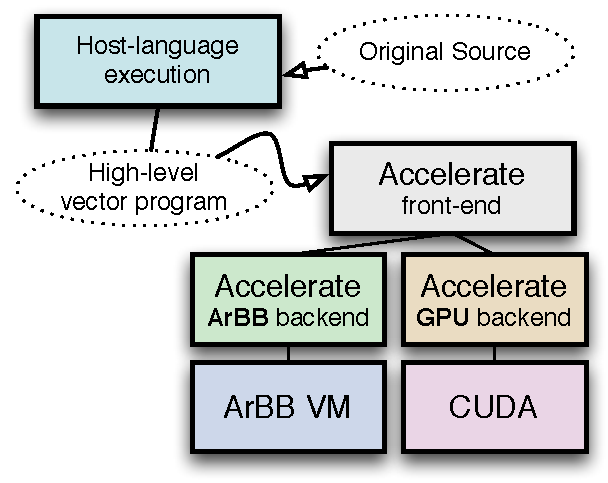
\includegraphics[width=2.0in]{./arbb/figure_architecture}    
  \end{center}
\vspace{-5mm}
  \caption{Architecture of the \systemname{} system.  \rn{(ROUGH.)}}
  \label{f:architecture}
\end{figure}


Using Accelerate and ArBB together, we propose a layered architecture
for \systemname{},
% Our goal is to make the benefits of ArBB available to the Haskell programmer. 
% \js{(Or is our goal to give an even better ``front-end'' to ArBB compared to C++)}
% We propose that this is best accomplished using a layered approach, as
pictured in Figure~\ref{f:architecture}. 
The host language execution (via Haskell in this case) executes the
programmer's source code, generating a vector program in the
restricted language of the Accelerate front-end.
Then either Accelerate backend---ArBB or CUDA---may be used.
The 
bottom layer of the ArBB backend consists of a direct mapping of the ArBB virtual machine
API (VMAPI) into Haskell including one-to-one bindings for each C 
function. 
To [partially] automate the creation of these bindings we used the C2HS system \citearbb{C2HS}. The 
\arbbvmH{} bindings are very low-level.
%and make little use of the high-level programming methods that
% Haskell programmers want. 
The idea 
is that the \arbbvmH{} bindings should be used to implement
backends for higher-level data-parallel EDSLs.

%% To illustrate our position we 
%% have started working on a backend to the successful DSL Accelerate 
%% (Data.Array.Accelerate) using our \arbbvmH{} bindings. 

To address the functionality mismatch between Accelerate and ArBB,
when possible we reencode the users Accelerate program using existing
ArBB mechanisms.  Our prototype does not support 100\% of Accelerate's
compute model (for example, only supporting  up to three-dimensional
arrays), but the remaining functionality can be mapped onto ArBB in
time using known methods---for example, our compiler could map higher
dimensional arrays onto a specific lower-dimensional data-layout.

%% The programming models supported by ArBB and Accelerate are very similar. 
%% Both obtain their parallelism by exposing collective operations 
%% such as {\em Map}, {\em Reduce}, {\em ZipWith} and {\em Scan} (all prefixes operations). However, 
%% the functionality match is not 100\%. For example, Accelerate supports {\em Map} operations 
%% over N-dimensional Arrays while ArBB supports them only up to 3-dimensions. 
%% Similar inconsistencies apply to the other operations as well. \textred{The current
%% ArBB backend simply disallows Accelerate programs using too high dimensionality
%% of the arrays.} \rn{Sure, we want to say that we're not done closing
%%   this gap (for
%%   accuracy) but more importantly we want to identify whether
%%   techniques exist to close the gap.  Presumably, yes?  We can
%%   ourselves collapse the dimensionality of arrays before giving them
%%   to ArBB?  Are there any operations that would defeat that technique?}
%

One example of a functionality discrepancy bridged by our
implementation is reductions.  As mentioned in \ref{sec:arbb},
Accelerate allows the programmer to reduce using an arbitrary
associative function, but ArBB has only built-in reductions with fixed
operations (add, multiply, xor, etc). We plan to provide general reductions in
the ArBB backend by a two-fold strategy:

\begin{enumerate}
\item Attempt to map an Accelerate reduction directly onto an ArBB
  primitive such as \cde{add\_reduce}.
\item Apply a general reduction technique based on $log(N)$ map
  operations over successively halving array sizes.  Essentially, cut
  the array in half, combine the halves, repeat. In ~\citearbb{reduction}
  this approach is explained in the context of CUDA. 
\end{enumerate}

%% \rn{Is the technique worthy of
%%   description?  Can we just cite the CUDA documentation or something
%%   since it's common?} 

In our current experiments, approach (2) is significantly slower.
Therefore, the ideal would be that ArBB exposed general reduction
directly in its programming model.  We expect this functionality to be
added in future releases.  In the meantime we plan to explore a
technique that would allow us to maximize the number of situations in
which (1) above applies.  Namely, a reduce operation can often be {\em
  factored} into a map followed by a reduce.  For example, a reduction
that multiplies each input number by a coefficient and sums the
results can be split into a map phase for the multiplication followed
by the built-in \cde {add\_reduce} operator.

%% Currently, our reduction implementations in ArBB 
%% are many times 
%% slower (\textasciitilde 20x) than their built-in counterparts. 
%% % To ameliorate this present performance problem we attempt to map
%% % programmers 
%% Our present workaround for this performance problem is to let 
%% \accarbb{} inspect the reduction function and switch to efficient 
%% built in  ArBB reduction where possible.  
%% \rn{Future work may be to decompose reductions into map+reduce so as
%%   to allow the reduce to become a builtin.}


Another choice faced by our implementation is the granularity at which the
ArBB JIT is invoked.  Specifically, should each collective operation result in its
own call to the ArBB JIT (in ArBB terminology, {\em
  immediate-mode}, akin to the pre-OpenGL 3.0 immediate mode), or
should multiple collective operations be placed together
inside an ArBB function and passed to the JIT?
We will call the latter approach {\em retained-mode}.

%% In immediate-mode the 
%% operations called from the ArBB API are executed
%% synchronously---before each API call returns. In retained-mode, ArBB
%% collects calls and, only when results are requested, the 
%% entire computation is optimized 
%% and executed. 

Retained-mode generally offers performance benefits; a bigger 
chunk is given to the JIT compiler, enabling cross-optimization
between collective operations. 
Our prototype Accelerate backend uses 
ArBB in  
a combination of immediate- and retained-mode. The main collective 
operations are compiled using the retained-mode. For example, in the case 
of a \cde{map f}  operation first the function to be mapped is created and 
compiled using retained-mode then a small {\em mapper} function is 
also created and compiled using retained-mode. 
%% The mapper function is 
%% of course very small and therefore does not give much to the JIT compiler 
%% to work on optimization-wise. 
Between the collective operations the backend
needs to perform data management and copying, which 
are performed in immediate-mode. It is our belief that 
\systemname{} would benefit from using retained-mode exclusively 
but we leave that as future work. 





% ====================================================================================================
\subsection{Preliminary Results}
% ====================================================================================================

%\rnote{One tiny benchmark if we can manage it.}

%\rnote{Ideally: Something like blackscholes running Arbb/C++,
%  \systemname{}, CPU+GPU, possibly compared to other blackscholes
%  implementations -- say Cilk on CPU and hand-coded CUDA (I can
%  provide the former I think).  Perhaps serial, non-vectorized CPU for
%  comparison.}

%\rnote{Point 1 -- High level thing is within X\% of low level thing.
%  The usual.  But we also want to say that \systemname{} is no worse
%  than ArBB/C++ -- the metalanguage doesn't matter, be it Haskell,
%  Python, or C++.}

%\rnote{Point 2 -- It's important to do a good job on the CPU side.
%  Even if you don't beat GPU there's a big difference between
%  vectorizing/not-vectorizing (and using multicore of coarse).  Can't
%  be ignored.}

%\rnote{Bonus points -- if we could show how bad ``naive'' ports are that
%  would be nice.  How well does your C CPU code run on GPU unmodified
%  (or minimally ported)?}



%\rnote{CPU/GPU systems that do a good job of both.  Perhaps quickly
%  dismiss those that make no effort on the CPU side.}

Black-Scholes option pricing is a finance-related benchmark that has been used in similar
DSLs targeting GPUs \citearbb{ACCELERATEDAMP11, NIKOLA}. Since we are re-using the 
Accelerate front-end, we can directly use the Black-Scholes benchmark that 
is shipped with that system.  Figure \ref{fig:blackscholes} shows the
complete code listing for an Accelerate Black-Scholes function which
can be executed on GPUs or any processor targeted by ArBB.

% blackscholes :: Vector (Float, Float, Float) 
%
%                -> Acc (Vector (Float, Float))
%\fbox{

%       r     = \textit{constant} riskfree
%       v     = \textit{constant} volatility

\begin{figure}
\begin{footnotesize}
\begin{Verbatim}[frame=single, commandchars=\\\{\}]
blackscholes (xs :: Vector (Float,Float,Float)) = 
  map kernel (\textit{use} xs)

kernel x =
  \kw{let} (price, strike, years) = \textit{unlift} x
      r     = 0.02 \textsf{\textit{-- riskfree constant}}
      v     = 0.30 \textsf{\textit{-- volatility constant}}
      sqrtT = sqrt years
      d1    = (log (price / strike) + 
                   (r + 0.5 * v * v) * years) / 
              (v * sqrtT)
      d2    = d1 - v * sqrtT
      cnd d = d >* 0 ? (1.0 - cndfn d, cndfn d)
      cndD1 = cnd d1
      cndD2 = cnd d2
      expRT = exp (-r * years)
  \kw{in} \textit{lift} ( price * cndD1 - 
            strike * expRT * cndD2
          , strike * expRT * (1.0 - cndD2) - 
            price * (1.0 - cndD1))

cndfn d =
  \kw{let} poly  = horner coeff
      coeff = [0, 0.31, -0.35, 1.78, -1.82, 1.33]
      rsqrt = 0.39894228040143267793994
      k     = 1.0 / (1.0 + 0.2316419 * abs d)
  \kw{in} rsqrt * exp (-0.5*d*d) * poly k

horner coeff x = 
  \kw{let} madd a b = b*x + a
  \kw{in}  foldr1 madd coeff
\end{Verbatim}
\end{footnotesize}
\caption{Complete code listing for a Black-Scholes function expressed
  in Haskell syntax using the Accelerate and \systemname{} libraries.
  Invocations of the functions \cde{use}, \cde{lift} and \cde{unlift}
%  and \cde{constant} 
represent additional boilerplate added for
  conversion in and out of Accelerate types.  Specifically, \cde{lift} and
  \cde{unlift} convert tuples and handle the fact that Accelerate
  arrays of tuples are really implemented as tuples of arrays.
  Otherwise, the program is identical to a plain Haskell
  implementation.}
\label{fig:blackscholes}
\end{figure}


%% \end{code}
%%  %605993438
%% % horner :: Num a => [a] -> a -> a
%% \begin{code}
%% \footnotesize



The kernel of this algorithm performs arithmetic on triples of
floating point numbers, creating pairs of floats as results. The problem 
is embarrassingly parallel, consisting of independent computations
for every element of an array (a map).

\begin{figure}
  \begin{center}
   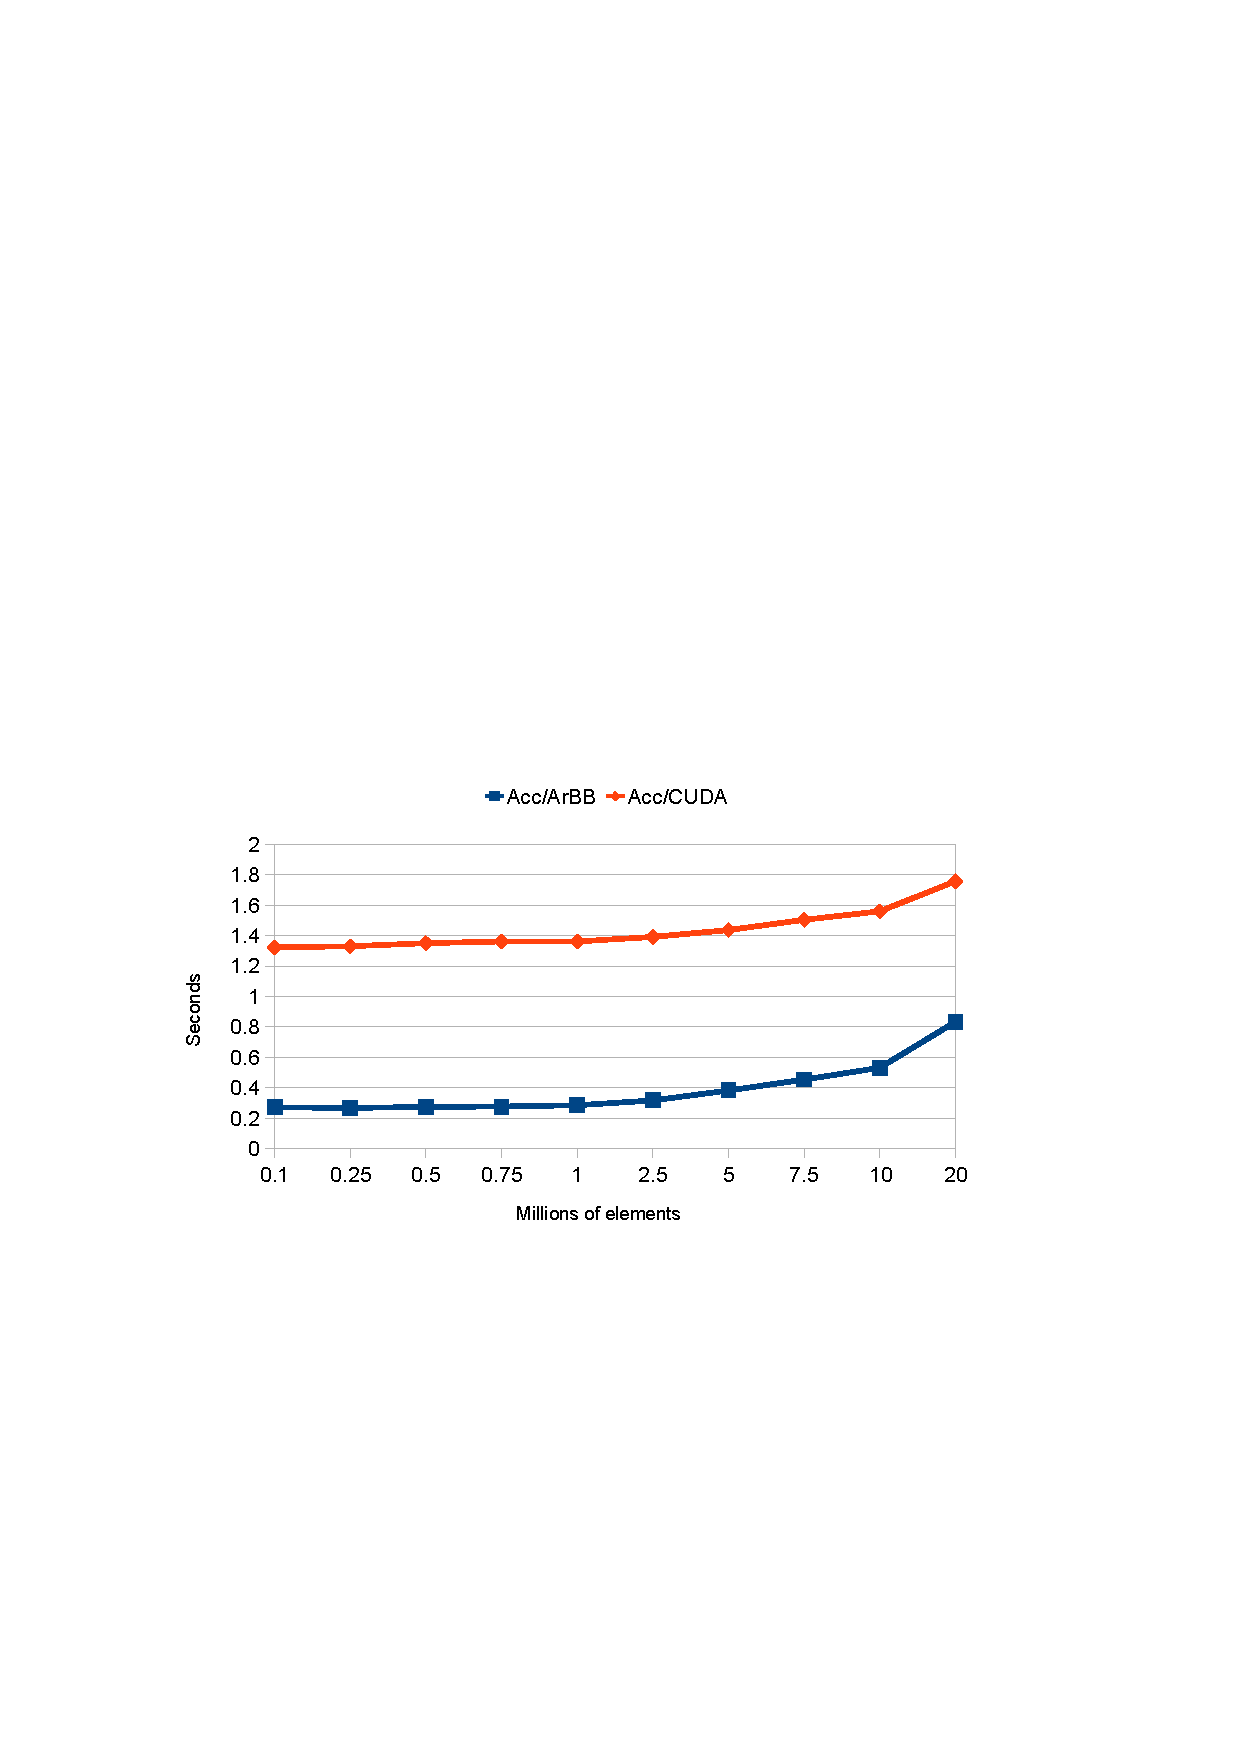
\includegraphics[width=3.5in]{./arbb/jit}    
  \end{center}
\vspace{-5mm}
  \caption{Running time experiments including JIT-time.} 
  \label{f:jit}
\end{figure}

\begin{figure}
  \begin{center}
   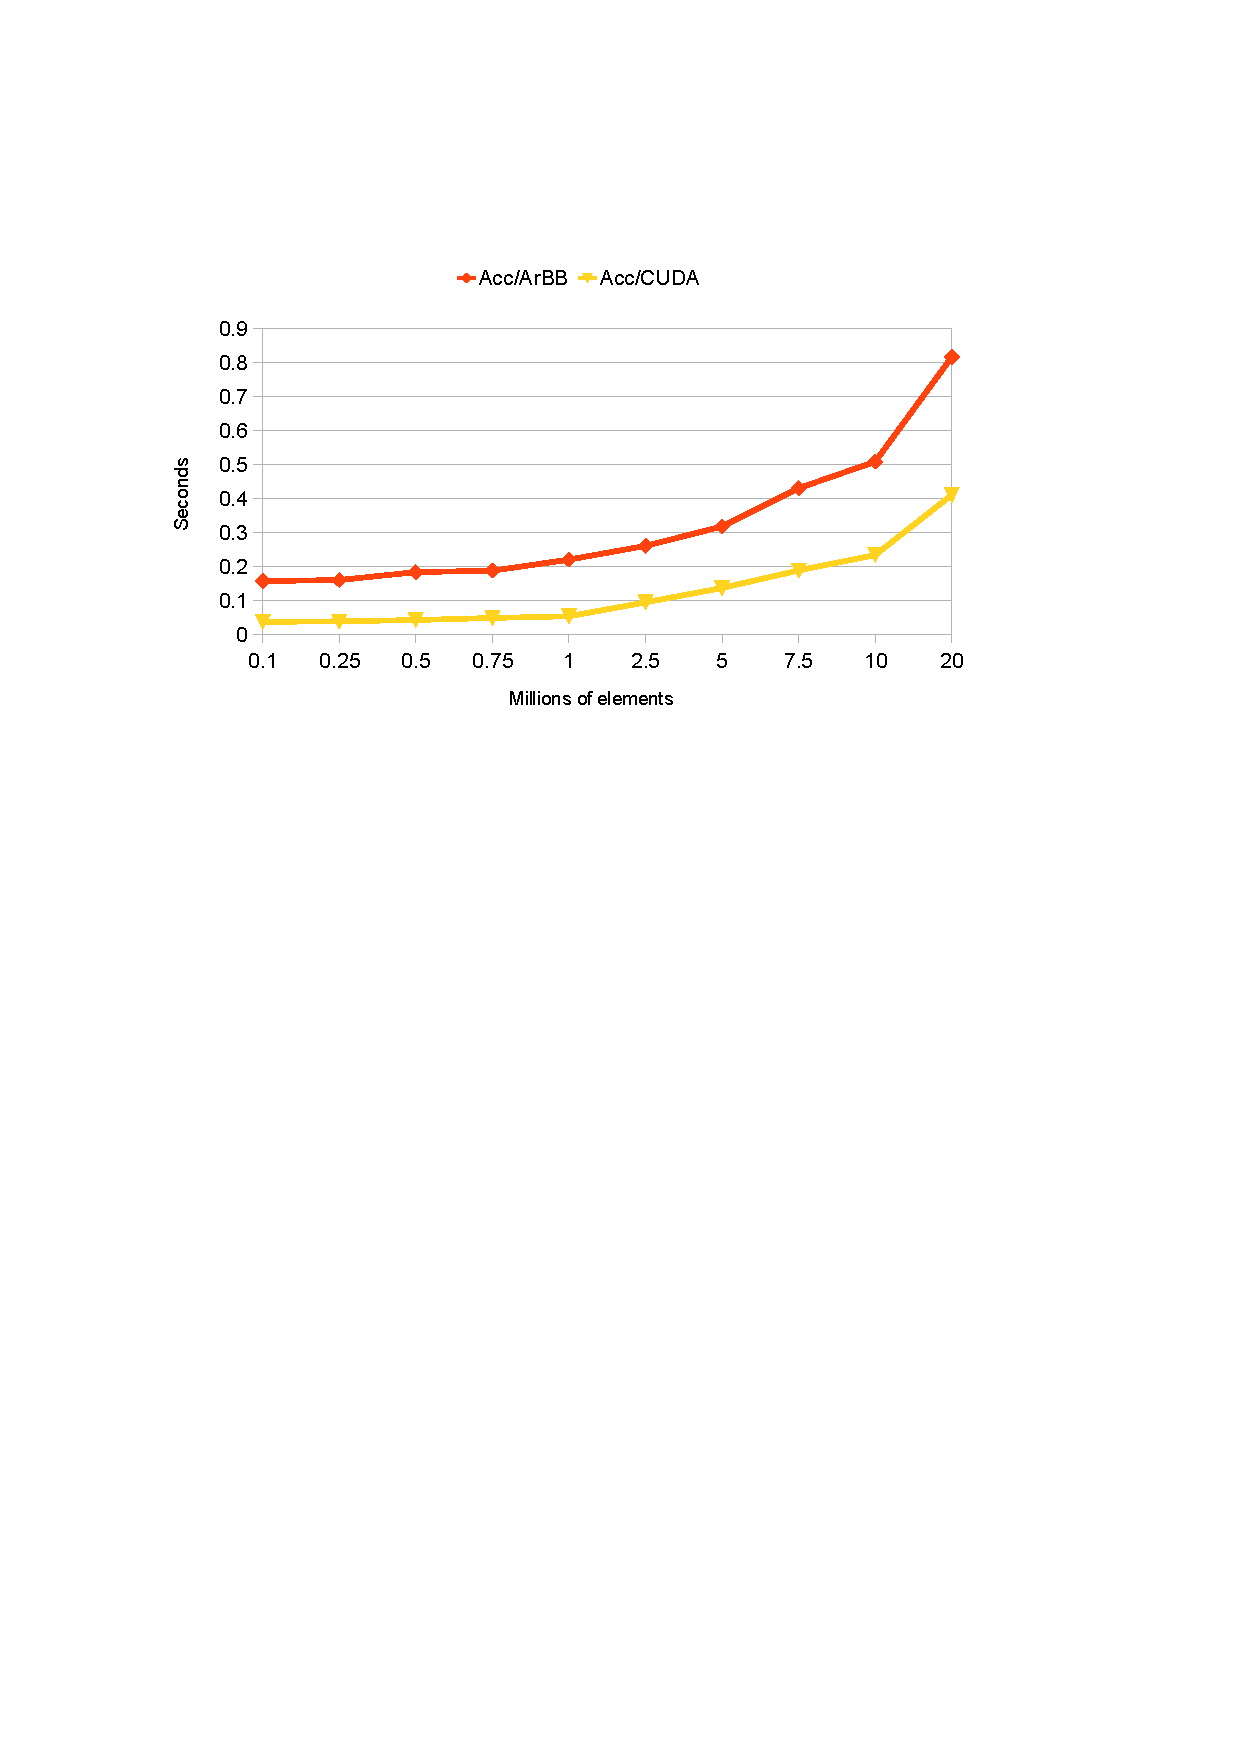
\includegraphics[width=3.5in]{./arbb/nojit}    
  \end{center}
\vspace{-5mm}
  \caption{Running time experiments JIT-time excluded.}
  \label{f:nojit}
\end{figure}


Figures~\ref{f:jit} and \ref{f:nojit} show preliminary results obtained on 
the Black-Scholes benchmark. The figures where obtained on a system with a 4-core 
Intel Core I7 975 machine with HyperThreading. The GPU used was a NVIDIA GTX480.

Figure~\ref{f:jit} shows running times obtained when JIT-time is included. 
% What this figure mainly tells us is that the JITing overhead 
JIT compilation time is much larger 
in the CUDA backend than the ArBB one.  Part of this difference 
can be attributed to the fact that 
the CUDA backend calls an external compiler (\cde{nvcc}), which takes its input in a file and runs in
a separate process.  ArBB, on the other hand, has a library interface to its  JIT-compiler. 
Figure~\ref{f:nojit} shows results obtained when pre-compiling the
CUDA functions eliminating JIT overhead.
In Accelerate, this happens automatically when the same kernel is
invoked repeatedly, because the Accelerate CUDA backed 
uses a caching scheme to avoid unnecessary JIT invocations.  (The
caching functionality has not yet been duplicated in the 
ArBB backend.)

These early results demonstrates the principle that even when a kernel
executes with higher throughput on a GPU, in a particular program it
is difficult to decide whether a computation is worth moving to a GPU,
incurring extra data-movement and possibly extra JIT compilation
\citearbb{wheres-the-data-paper}.  Specifically, we see that the
Accelerate Black-Scholes program from Figure~\ref{fig:blackscholes}
performs better on the CPU if it executes once (even on a large window
of data) whereas the GPU would yield better performance in a sustained
series of executions.
%
Because both CPU and GPU execution may be desirable---and the
selection may be dynamic---it is beneficial to have a single source code
that is portable across both.  
% Accelerate combined with \systemname{} makes this possible.


% ====================================================================================================
\subsection{Related Work}
% ====================================================================================================


OpenCL~\citearbb{opencl08} is a programming model very similar to CUDA but with the aspiration 
to offer both acceleration of computations on GPUs or to multicore CPUs. 
OpenCL JIT compiles the kernels for the particular hardware available and is
in that sense similar to ArBB.  
OpenCL programs are relatively low-level and require a large amount of
boilerplate to create and invoke.  In this sense they occupy a very
different niche than Accelerate.

Microsoft Accelerator~\citearbb{ACCELERATOR} is an embedded language with similar 
aspirations as ArBB, that is, to target a diverse range of architectures using the 
same source code. Accelerate can be used from the C\# language or the 
functional F\# language and targets GPUs or of CPUs and their
vector units.
% However, being part of the .Net framework implies limited accessibility 
%for platforms other than Microsoft Windows.  

\rn{What's the comparison with our stuff?}

%Most work on partitioning workloads between 
Many CPU and GPU comparisons, and some CPU/GPU workload partitioners \citearbb{merge}, rely on
redundant hand-written versions of all kernels
% \citearbb{cpu-gpu-partitioning} 
(though some systems like Qilin \citearbb{qilin} allow a single source code).
It is difficult in this kind of scenario
to make fair comparisons, controlling for the
amount of effort put into the respective implementations.
For example, comparing unoptimized serial CPU implementations vs. GPU
ones is not informative \citearbb{debunking-dubey}.
In \systemname{} controlling for effort
need happen only once---both CUDA and ArBB are
independently optimized by their respective teams of engineers---not for each benchmark.


% ====================================================================================================
% \section{Future work and Conclusions}
%\section{Future Work}
% ====================================================================================================

%\rn{need to be careful about being too repetitive...}
%The \accarbb{} backend is currently work-in-progress. The Accelerate
%functionality is not yet completely covered by the ArBB backend. Currently 
%the ArBB back-ed is operational for Accelerate programs using {\em Map}, 
%{\em ZipWith} and some simple instances of the Accelerate {\em Fold} operation.
%All of these also have the limitation that they only work for up to and 
%including 3-dimensional arrays using the ArBB backend while the Accelerate
%model allows the N-dimensional case. Allowing the N-dimensional case 
%in the ArBB backend for the supported operations range from a simple exercise 
%to more intricate problems needing some thought. For example, in the case 
%{\em Map} operations the needed transformation is simple (Accelerate Maps 
%over N-dimensional arrays is a per-element operation). One could flatten 
%the N-dimensional array to a 1-dimensional array (remembering its old shape) 
%perform the map and then transform the array back into N-dimensions. In 
%the case of {\em Fold} (reductions) the situation becomes more tricky. 
%transforming the arrays to arrays of lesser dimensionality then requires 
%a so-called segmented {\em Fold} operation. 

%The current \accarbb{} backend uses a hybrid of immediate-mode 
%and retained-mode programming styles. Moving more towards 
%retained-mode only may have performance benefits since it would give the 
%ArBB compiler larger programs to optimize. Exploring this aspect is left 
%as future work. 

% ====================================================================================================
\subsection{Discussion and Conclusions}
% ====================================================================================================

We have demonstrated that an EDSL such as Accelerate is sufficiently
platform-independent to break free of its original hardware target
(CUDA/GPU) and create efficient programs on other architectures.  This
gives us hope that \systemname{}/Accelerate programs will be
forward-portable to future parallel architectures and instruction
sets.

The EDSL approach changes the playing field for the designer
of compiler backends.  Rather than contending with full blown
languages and their complexities (e.g. pointers, aliasing,
inheritance, virtual functions, etc), compiler backends can focus on
simple value-oriented compute languages.

%% Achieving the ultimate goal of performance portability requires
%% progress on two research problems.  The first is EDSLs themselves and
%% their integration into host languages.  The second problem 

But the EDSL method solves only part of the performance-portability problem.
Simple as EDSL target languages may be, there remains a
substantial challenge in mapping them efficiently to the diversity
of parallel architectures available now and in the near future.
%especially without requiring a large amount of additional per-platform
%user annotations.
\textred{For example, the idiosyncrasies of memory bank access on
  NVIDIA GPUs must be taken into account to generate efficient
  implementations of the high-level collective operations that we have
  discussed.}

This is a compiler backend research challenge.
The {\em skeletons} method mentioned in
Section~\ref{sec:accelerate-arbb} is one approach to this problem, as
are the optimizations studied in the Copperhead \citearbb{copperhead} and
Obsidian \citearbb{JSLIC} projects.
%
On the other hand, systems that rely on advanced optimizations
typically suffer to some extent from performance-predictability
problems.  Thus achieving portable, predictable performance on a wide range
of architectures---even for the simplest target languages---will
be the subject of much future work.

%{
%\small
\bibliographystylearbb{alpha}
\bibliographyarbb{thesis}
%}


%\end{document}




% ---------------------------------------------------------------------------
% 
% ---------------------------------------------------------------------------
\cleardoublepage 


\section[\paperHTitle]{\paperH: \\ \paperHTitle}
\label{sec:paperH}
%\addcontentsline{toc}{chapter}{Parallel Programming in Haskell Almost for Free}

% \paperHTitle

\begin{center} 
Bo Joel Svensson, Mary Sheeran
\end{center}



%% bare_conf.tex
%% V1.3
%% 2007/01/11
%% by Michael Shell
%% See:
%% http://www.michaelshell.org/
%% for current contact information.
%%
%% This is a skeleton file demonstrating the use of IEEEtran.cls
%% (requires IEEEtran.cls version 1.7 or later) with an IEEE conference paper.
%%
%% Support sites:
%% http://www.michaelshell.org/tex/ieeetran/
%% http://www.ctan.org/tex-archive/macros/latex/contrib/IEEEtran/
%% and
%% http://www.ieee.org/

%\documentclass[conference]{IEEEtran}

%\usepackage{graphicx, color, code}
%\usepackage[cmex10]{amsmath}
%\usepackage{url}
% \usepackage{bookman}  %% bold teletype fonts, but don't know how to prevent it from changing the whole document

% Haven't figured out how to get this to work properly:
%\usepackage[\texttt{cmbtt}]{bold-extra}
% \usepackage{bold-extra} 

%\usepackage{courier}
%\usepackage{fancyvrb}

% correct bad hyphenation here
%\hyphenation{op-tical net-works semi-conduc-tor}


%====================================================================================================
%% FIRST, MISC USEFUL DEFINITIONS
%====================================================================================================

\definecolor{darkgreen}{rgb}{0, 0.5, 0}
\definecolor{darkblue}{rgb}{0,0,0.5}
\definecolor{mygrey}{rgb}{0.7,0.7,0.7}
\newcommand{\textblue}[1]{\textcolor{blue}{#1}}

\newcommand{\cde}[1]{{\footnotesize \tt #1}}

% \newcommand{\kw}[1]{{\bf{#1}}}
\newcommand{\kw}[1]{{\textbf{#1}}}

\newcommand{\comm}[1]{{\em \textcolor{darkgreen}{#1}}}  %% Code comments

\newcommand{\note}[1]{\begin{itemize}\item \textcolor{blue}{#1} \end{itemize}}

%% \newenvironment{mycode}
%% {% This is the begin code
%%   \begin{Verbatim}[commandchars=\\\{\}]}%
%%   %\footnotesize
%%   %\noindent
%%   %\begin{code}\noindent\vspace{-1mm}}
%% %  \begin{code}\noindent}
%% {% This is the end code
%%   \end{Verbatim}
%%   %\end{code} 
%% }

%% \newenvironment{inlinecode}
%% {
%%   \begin{center}
%%   \begin{minipage}{4in}
%%   \begin{mycode}
%% } 
%% {
%%   \end{mycode}
%%   \end{minipage}
%%   \end{center}
%%   \vspace{-1.5ex}
%% }

%% ============================================================
%% USE TO DISABLE COMMENTS:
 \def\noeditingmarks{}
%% ============================================================
\ifx\noeditingmarks\undefined
   \newcommand{\textred}[1]{\textcolor{red}{#1}}
   \newcommand{\pgwrapper}[2]{\textred{#1: #2}}
%   \newcommand{\pgwrapper}[2]{}
   \newcommand{\rnote}[1]{\begin{itemize}\item{\textcolor{blue}{#1}}\end{itemize}}
   \newcommand{\new}[1]{\textcolor{blue}{#1}}
   \newcommand{\const}[1]{\textred{#1}}

%% RRN: Dim the background for Ryan's eyes:
%%   What I need here is a way to do it based on user or host name...
% \pagecolor{mygrey}

\else
   \newcommand{\textred}[1]{#1}
   \newcommand{\pgwrapper}[2]{}
   \newcommand{\rnote}[1]{}
   \newcommand{\new}[1]{#1}
   \newcommand{\const}[1]{#1}
\fi

\newcommand{\js}[1]{\pgwrapper{BJS}{#1}}
\newcommand{\rn}[1]{\pgwrapper{RRN}{#1}}


%% Can we call our ``things'' 
%% ArBB/Haskell for the bindings part ? 
%% Accelerate/ArBB for the Accelerate backend ?
%% This would work with the convention we adopted for 
%%      ArBB/C++  
\newcommand{\systemname}[0]{{Harbb}}
%\newcommand{\systemname}[0]{\textred{HArBB}}

%% This could in theory be separate from the project name..
\newcommand{\accarbb}[0]{\systemname{}}

%% NOTE: THIS SHOULD BE THE SAME AS SYSTEMNAME:
\newcommand{\arbbvmH}[0]{ArBB/Haskell}


%====================================================================================================
% END DEFINITIONS
%====================================================================================================




%\begin{document}
% \title{Painless Portable Vector Parallelism\\ with Haskell and Intel ArBB}
%\title{Programming Future Parallel Architectures\\ with Haskell and Intel ArBB}
% \title{Embedded Domain-Specific Languages Pave the Way for New Parallel Architectures}

%\author{\IEEEauthorblockN{Bo Joel Svensson}
%\IEEEauthorblockA{Dept. of Computer Science and Engineering\\
%Chalmers University of Technology\\
%Gothenburg, Sweden\\
%Email: joels@chalmers.se}
%\and
%\IEEEauthorblockN{Ryan Newton}
%\IEEEauthorblockA{Intel Corporation\\
%Hudson, MA\\
%Email: rrnewton@gmail.com
%}}
% Email: ryan.r.newton@intel.com

%\maketitle

%\begin{abstract}
%
\subsection*{Abstract}
New parallel architectures, such 
\new{as Cell, Intel MIC, GPUs, and tiled architectures, enable} high
performance but are often hard to program.
What is needed is a bridge between high-level programming models 
where programmers are most productive and modern parallel architectures. 
We propose that that bridge is Embedded Domain Specific Languages (EDSLs). 

\new{One attractive target for EDSLs is}
Intel ArBB, a virtual machine for parallel, vectorized computations.
% that serves as a compilation target for EDSLs.
We propose to wed ArBB with the functional programming language
Haskell, {using an EDSL} that generates code for the ArBB VM.  This Haskell integration provides 
% a determinism guarantee 
added safety guarantees compared to other ArBB interfaces.
%
Further, our prototype, \systemname{}, is one of the first EDSL implementations with
optimized backends for multiple parallel architectures (CPU, \new{NVIDIA GPU}, and
others), allowing portability of source code over devices
and their accelerators.


%\end{abstract}
%\IEEEpeerreviewmaketitle




% ====================================================================================================
\subsection{Introduction}
% ====================================================================================================

Are radical new parallel architectures market-feasible if they require
significant changes for programmers?  The jury is out.  In recent
years we have seen difficult-to-program chips suffer 
% \citearbb{cell} 
(e.g. Cell)
and
GPU vendors strive to enable more traditional programming features
\citearbb{fermi} (e.g. C++).  There is an increasing
tension between ease of programming and efficiency.

The tension  shows  across diverse chip markets.  For example,
small embedded devices are most power efficient if their processors and operating systems
omit programming features such as virtual memory and threads \citearbb{tinyos}.  
At the other end of the power spectrum, GPU's
graphics performance may suffer due to inclusion of hardware to ease
GPGPU programming.  In short, there is an opportunity cost to
including extra hardware for programmability.

In this paper, we argue 
that a specific technique holds the greatest promise of solving the programmability dilemma.
%
Domain-specific languages, {\em embedded} within general purpose
languages (EDSLs) 
 enable familiar programming models 
{\em and} flexible
mapping onto new hardware.  The key to having this cake and eating it
too is {\em metaprogramming}.  Familiar programming features are
present, but are eliminated at an intermediate (metaprogram evaluation)
phase and therefore do not reach the parallel hardware itself.


% We present our ongoing work on a
In pursuit of this vision, we offer a
% 
 new EDSL implementation, called \accarbb{}, that combines
existing systems, Accelerate \citearbb{ACCELERATEDAMP11} and ArBB \citearbb{ArBB}, to produce a unified
high-level programming environment equally suited to multicore,
vectorized CPUs, as to GPUs and other accelerators (such as Intel MIC chips \citearbb{larrabee}).
%
\if{0}
ArBB is based on the RapidMind \citearbb{RapidMind} system which was an embedded 
DSL targeting multicore CPUs as well as GPUs. ArBB does not \new{yet} include a GPU 
backend like RapidMind, targeting multicore CPUs and their vector 
units. 
\fi{}
\systemname{} is a single EDSL implementation 
with independently optimized backends \new{by different teams; 
namely, the ArBB backend for CPU/MIC, and a CUDA backend for NVIDIA GPU.}
This makes
\systemname{} an appealing platform for fair CPU/GPU comparisons, 
as well as a compelling programming model for single-source portable performance across a range of
parallel architectures, \new{present and future}.
%%To our knowledge, \systemname{} is the first EDSL implementation with
%%independently optimized backends for CPUs and GPUs.  This makes
%%\systemname{} an appealing platform for fair CPU/GPU comparisons, 
%%as well as a compelling programming
%%model for single-source portable performance across a range of
%%parallel architectures.


% ====================================================================================================
\subsection{Embedded Domain-Specific Languages}
% ====================================================================================================


Domain-specific languages---from Makefiles and \LaTeX{} to
Matlab---are almost too ubiquitous to notice.  Most relevant to our
purposes, domain-specific languages (DSLs) that target a narrow domain and expose communication
patterns to the compiler 
 have achieved performance-portability across a wide range of parallel
architectures.  
StreamIt\citearbb{streamit} is a good example.
% (for example, StreamIt\citearbb{streamit})
% The high-water mark in this area is perhaps  StreamIt\citearbb{streamit}.
% 

% It has been noted \citearbb{not-sure} that 
% Yet the few DSLs that gain popularity lose simplicity\citearbb{not-sure}.  
% Yet popular DSLs rarely remain simple \citearbb{not-sure}.  
DSLs may start out simple and focused, but if they gain popularity
they quickly grow in complexity to rival full-blown languages.
Feature creep
can make DSL implementations complex and expensive to maintain.
Further, non-standard DSL syntax and features present a learning curve for users.  In the
last ten years an attractive solution to this dilemma has emerged: {\em
  embed} each DSL into a general-purpose host language that can provide
common functionality with familiar syntax and semantics.
% in place of the DSL.

When embedding, host language programs {generate} DSL programs;
% Embedding means that the host language is used to generate DSL programs; 
the {\em deeper} the embedding, the more integrated the
DSL into the syntax and type-system of the host language.
%
% Typically, %% pruning weasel words
A key host-language feature for embedding is that
language constructs can be overloaded to operate over {\em abstract
  syntax trees} (ASTs)\footnote{This ad-hoc polymorphism is accomplished,
for example, through operator-overloading in C++ or type classes in
Haskell.}.  For example, the following simple function operates on scalars:


\vspace{1mm}
\begin{Verbatim}[commandchars=\\\{\}]
  float f(float x) \{ return (2*x - 1); \}
\end{Verbatim}
\noindent
But simply by changing the types, \cde{f} might be lifted to operate on {\em
  expressions} (which, when evaluated, will yield \cde{floats}):

\vspace{1mm}
\begin{Verbatim}[commandchars=\\\{\}]
  \kw{exp<float>} f(\kw{exp<float>} x) \{
    return (2*x - 1);
  \}
\end{Verbatim}

A common arrangement is for the host language program to execute at
runtime but to generate ASTs that are executed by a just-in-time
(DSL) compiler.  This use of metaprogramming (program generation)
differs from the more common usage of preprocessors and 
% Lisp/Scheme macros \citearbb{scheme-macros}
macros, which typically add extra
phases of computation {\em before}  compile time---increasing
the number of compile-time rather than runtime phases.

% EDSLs typically add additional runtime phases.  That is, the host language program 
% executes at runtime but uses a JIT to process generated ASTs.
%% which are
%% usually used to perform computation {\em earlier} than the usual
%% compile time, embedded DSLs (EDSLs) typically defer computation 


One reason that EDSLs are good for productivity is that the programmer
gains the software engineering benefits of the host language
(object-orientation, higher-order-functions, modules, etc), while not
paying the cost at runtime for additional layers of abstraction or
indirection.  Indeed, the embedded languages for 
performance-oriented EDSLs are often simple, first-order
languages without pointers \citearbb{wavescript, ACCELERATEDAMP11}.

% , paul-lius-thingy

% regiment,
As a research area, EDSLs and two-stage DSLs have been actively pursued for at least a
decade \citearbb{VERTIGO, wavescript} but are gaining steam
recently 
%\citearbb{sejits, stanford-ppl} 
\citearbb{copperhead, stanford-ppl} 
and are beginning to appear in
commercial products \citearbb{ArBB}.
%
Further, EDSL techniques have spread beyond their origin in 
 the programming languages community.
% 
For example, both Stanford's Parallel Programming Laboratory (PPL) and
the Berkeley Parlab are creating EDSLs as their flagship parallel
programming solutions for domains such as machine learning and
rendering \citearbb{stanford-ppl}.
  Moreover, EDSLs need not be hosted by esoteric research languages---Intel's
 ArBB embeds an array language in C++ and Berkeley's
Copperhead \citearbb{copperhead} generates CUDA from simple Python code.

%\rnote{Is there a good motivating example program?  What are some of
%  the Metaocaml motivating examples?}

{For the remainder of this paper we will focus our discussion
  on the Intel ArBB VM, a virtual machine for just-in-time
  generation of vector codes, \new{which implements a restricted} domain-specific
  language of array computations.  In this paper we introduce
  {\em High-level ArBB}, 
  (\systemname{}), an EDSL that internally uses the ArBB
  VM.  \new{While Intel's ArBB package already includes an EDSL targeting the VM (for C++)},
\systemname{} \new{offers additional advantages, including}
  more succinct programs and additionally safety
  guarantees---namely, complete deterministic-by-construction parallel
  programs (across both host and VM languages).}


% ====================================================================================================
% \section{Accelerate and ArBB}
%\section{\accarbb{}:  ArBB and Accelerate}
\subsection{\accarbb{} $=$ ArBB $+$ Accelerate}
\label{sec:accelerate-arbb}
% ====================================================================================================

Our first \systemname{} prototype adapts an existing EDSL called {\em
  Accelerate} (Data.Array.Accelerate).  Accelerate targets high-level
data-parallel programming in Haskell.
Previous work on Accelerate has focused on developing a CUDA-backend
for GPU programming.  In this paper we describe our effort to retarget
Accelerate to ArBB.  

With respect to determinism guarantees, the existing Intel ArBB product
represents an integration of the safe (ArBB VM) with the unsafe (C++).
In the Haskell context, because purely functional computations are
guaranteed deterministic (even when executed in parallel), and because
ArBB computations invoked by Haskell functions are themselves free of
side-effects, \systemname{} achieves a
guarantee of determinism for complete programs that combine both
Haskell computation and ArBB VM computation.
% which offers portability.
% (The 'H' in \systemname{} therefore stands for Haskell as well as ``High-level''.)


%% {\em Accelerate} (Data.Array.Accelerate) is an existing EDSL for 
%% high-level data-parallel programming in Haskell~\citearbb{Accelerate}. 
The Accelerate programming model consists of collective 
operations that can be performed over arrays, together with a simple 
language of scalar expressions\new{---in the current release, the Haskell type system enforces that parallelism not be nested.}
\if{0}
The Haskell type 
system is used to enforce that no nested data-parallelism can be expressed 
\new{(in the current release, this may be relaxed in the future).}
\fi{}
Accelerate's collective operations include {\em Map} (akin to parallel
for loops) {\em ZipWith} (a generalization of elementwise vector addition) and 
{\em Fold} (sum generalized)---familiar operations for programmers versed in the functional paradigm.
All of these collective operations are easily parallelizable. 
% In the case of {\em Map} and {\em ZipWith} the potential for parallelism is abundant.  

%% dotProd :: Vector Float -> 
%%            Vector Float -> 
%%            Acc (Scalar Float) 
\begin{Verbatim}[commandchars=\\\{\}]
dotProd (xs :: Vector Float) 
        (ys :: Vector Float) = 
  \kw{let} xs\_ = use xs 
      ys\_ = use ys 
  \kw{in}  fold (+) 0 (zipWith (*) xs\_ ys\_) 
\end{Verbatim}

The Accelerate code listing above specifies a function that takes two 1-dimensional 
arrays as inputs (of type \cde{Vector Float}, e.g. a vector of floats). The result of the function is a single
scalar. 
% (\cde{Scalar Float})
The \cde{use} function is applied to an array to convert it 
for use in the collective operations provided by Accelerate;
\cde{use} 
% is actually a function with type \cde{Vector a -> Acc (Vector a)} and 
may result in
copying the array to, for example, the GPU in the case of Accelerate's 
CUDA backend.  

After applying \cde{use} to bring in input data, the programmer then
constructs a data-parallel program from collective operations.
Above, \cde{fold} is a function that takes three arguments, 
here those arguments are \cde{(+)},  $0$ and \cde{zipWith (*) xs\_ ys\_}. 
\cde{zipWith}, in turn, is a function taking three arguments, \cde{(*)}, 
\cde{xs\_} and \cde{ys\_}. The \cde{zipWith} operation here applies pairwise 
multiplication to the two arrays and the \cde{fold} sums up all the elements 
into a single scalar. 

%\rn{Following para slightly redundant but ok...}
%Accelerate makes GPU programming accessible to the functional programmer 
%by offering a familiar set of operations. This set of operations also have 
%the beneficial property that they have inherent parallelism and are 
%easily implementable on the GPU. 

Accelerate's CUDA backend implements collective operations using
a hand-tuned ``skeleton'' for each operation (and possibly for
different hardware versions). The kernel---for example, the function
to mapped over the dataset---is 
instantiated into the body of the skeleton code. The resulting 
program is compiled using the NVIDIA CUDA compiler and dynamically linked 
into the running Haskell program.

%\subsection{Intel Array Building Blocks (ArBB)}
\subsection{Intel Array Building Blocks (ArBB)}
\label{sec:arbb}

%ArBB is embedded in the C++ programming language but it also exposes a 
%very low level API that is purely C. 
%{\em ArBB} (Array Building Blocks) is also an embedded DSL. 
The operations exposed by ArBB are similar to those of Accelerate. 
In ArBB, parallel computations are expressed using a set of built-in 
primitives. All vectorization and threading is managed internally by 
ArBB. The programmer uses collective operations with a clear semantics 
such as \cde {add\_reduce} that computes the sum of the elements in a given 
array. ArBB also has language constructions for control flow, conditionals
and loops. These operations have their usual sequential semantics and are not 
parallelized by the system, rather, only specific collective operations are executed
in parallel. 

Today's existing ArBB product is embedded in C++ and provides special
types for scalars and arrays (e.g. \cde{dense<f32>} rather than \cde{vector<float>}).
Using ArBB/C++ to express the dot product computation can be done 
as follows:

%\vspace{2mm}
\begin{Verbatim}[commandchars=\\\{\}]
\kw{void} dot\_product(\kw{const} dense<f32>& a, 
                 \kw{const} dense<f32>& b,
                 f32& c) 
{ 
  c = add\_reduce(a * b);
}
\end{Verbatim} 


% The above program takes two arrays of type \cde{dense<f32>} as input. 
% \cde{dense<f32>} specifies a 1-dimensional array of 32-bit floating
% point values. The result is a single 32-bit float.  

Note that arithmetic operators such as (*) are overloaded 
for to operate on arrays as well as scalars (e.g. \cde{a * b} above).
Thus, the above C++ function multiplies two arrays before summing them with \cde {add\_reduce}:

The code listing below is indicative to the amount of glue code needed to invoke an 
ArBB computation\footnote{In OpenCL and CUDA the glue code situation is even worse}. It shows how the dot product code is launched using {\tt call} and 
how data is bound, {\tt bind}, for use in ArBB. 

\vspace{2mm}
\begin{Verbatim}[commandchars=\\\{\}]
\kw{int} main() 
\{ 
  double a[SIZE];
  double b[SIZE];

  for ( \kw{int} i = 0; i < SIZE; ++i) \{ 
    a[i] = ...; b[i] = ...;
  \}
  dense<f32> va, vb;
  f32 vc;
  bind(va, a, SIZE); 
  bind(vb, b, SIZE); 
  call(dot\_product)(va, vb, &vc); 
  ...
\}
\end{Verbatim}


%\rnote{SPECIFICALLY ADDRESS THE FUNCTIONALITY GAP?  E.G general
%  reduce.  Any other examples?}

The model provided by Accelerate is slightly richer than that of ArBB.
Even the two very simple \cde {dot\_product} examples above manage to illustrate 
this. In Accelerate there is a more general reduction primitive called \cde {fold} 
where in ArBB there are specific reductions, \cde {add\_reduce}, \cde {mul\_reduce} 
and so on. Not visible in these small examples is another difference, Accelerate 
operations are generalized to arbitrary dimensions while ArBB operations are 
limited to 1, 2, and 3 dimensions (and 0, i.e. scalar). These differences aside,
the ArBB and Accelerate programming models are very similar.


% ====================================================================================================
\subsection{Implementation of \systemname{}} 
% ====================================================================================================


%\rnote{Sadly the Haskell details don't buy us much here... what are
%  the {\em conceptual} problems solved in mapping the Accelerate
%  abstraction to the ArBB one?  The data models are similar, but
%  there are always mismatches -- dimensionality support, missing
%  reduction.}

%\rnote{What is the technique that you are using to address these sorts
%  of problems?  Is there anything to say about it?}

\begin{figure}
  \begin{center}
   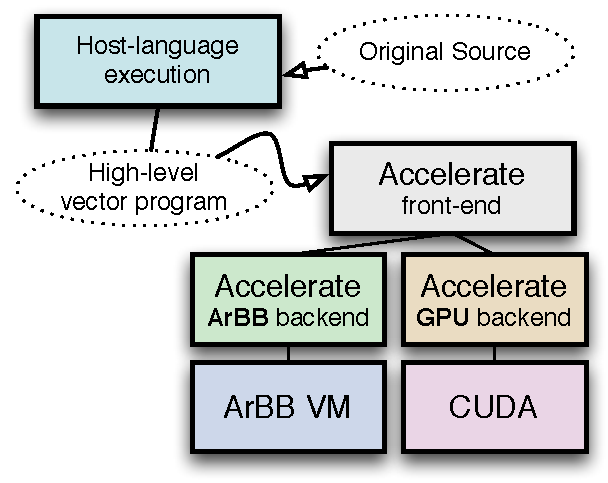
\includegraphics[width=2.0in]{./arbb/figure_architecture}    
  \end{center}
\vspace{-5mm}
  \caption{Architecture of the \systemname{} system.  \rn{(ROUGH.)}}
  \label{f:architecture}
\end{figure}


Using Accelerate and ArBB together, we propose a layered architecture
for \systemname{},
% Our goal is to make the benefits of ArBB available to the Haskell programmer. 
% \js{(Or is our goal to give an even better ``front-end'' to ArBB compared to C++)}
% We propose that this is best accomplished using a layered approach, as
pictured in Figure~\ref{f:architecture}. 
The host language execution (via Haskell in this case) executes the
programmer's source code, generating a vector program in the
restricted language of the Accelerate front-end.
Then either Accelerate backend---ArBB or CUDA---may be used.
The 
bottom layer of the ArBB backend consists of a direct mapping of the ArBB virtual machine
API (VMAPI) into Haskell including one-to-one bindings for each C 
function. 
To [partially] automate the creation of these bindings we used the C2HS system \citearbb{C2HS}. The 
\arbbvmH{} bindings are very low-level.
%and make little use of the high-level programming methods that
% Haskell programmers want. 
The idea 
is that the \arbbvmH{} bindings should be used to implement
backends for higher-level data-parallel EDSLs.

%% To illustrate our position we 
%% have started working on a backend to the successful DSL Accelerate 
%% (Data.Array.Accelerate) using our \arbbvmH{} bindings. 

To address the functionality mismatch between Accelerate and ArBB,
when possible we reencode the users Accelerate program using existing
ArBB mechanisms.  Our prototype does not support 100\% of Accelerate's
compute model (for example, only supporting  up to three-dimensional
arrays), but the remaining functionality can be mapped onto ArBB in
time using known methods---for example, our compiler could map higher
dimensional arrays onto a specific lower-dimensional data-layout.

%% The programming models supported by ArBB and Accelerate are very similar. 
%% Both obtain their parallelism by exposing collective operations 
%% such as {\em Map}, {\em Reduce}, {\em ZipWith} and {\em Scan} (all prefixes operations). However, 
%% the functionality match is not 100\%. For example, Accelerate supports {\em Map} operations 
%% over N-dimensional Arrays while ArBB supports them only up to 3-dimensions. 
%% Similar inconsistencies apply to the other operations as well. \textred{The current
%% ArBB backend simply disallows Accelerate programs using too high dimensionality
%% of the arrays.} \rn{Sure, we want to say that we're not done closing
%%   this gap (for
%%   accuracy) but more importantly we want to identify whether
%%   techniques exist to close the gap.  Presumably, yes?  We can
%%   ourselves collapse the dimensionality of arrays before giving them
%%   to ArBB?  Are there any operations that would defeat that technique?}
%

One example of a functionality discrepancy bridged by our
implementation is reductions.  As mentioned in \ref{sec:arbb},
Accelerate allows the programmer to reduce using an arbitrary
associative function, but ArBB has only built-in reductions with fixed
operations (add, multiply, xor, etc). We plan to provide general reductions in
the ArBB backend by a two-fold strategy:

\begin{enumerate}
\item Attempt to map an Accelerate reduction directly onto an ArBB
  primitive such as \cde{add\_reduce}.
\item Apply a general reduction technique based on $log(N)$ map
  operations over successively halving array sizes.  Essentially, cut
  the array in half, combine the halves, repeat. In ~\citearbb{reduction}
  this approach is explained in the context of CUDA. 
\end{enumerate}

%% \rn{Is the technique worthy of
%%   description?  Can we just cite the CUDA documentation or something
%%   since it's common?} 

In our current experiments, approach (2) is significantly slower.
Therefore, the ideal would be that ArBB exposed general reduction
directly in its programming model.  We expect this functionality to be
added in future releases.  In the meantime we plan to explore a
technique that would allow us to maximize the number of situations in
which (1) above applies.  Namely, a reduce operation can often be {\em
  factored} into a map followed by a reduce.  For example, a reduction
that multiplies each input number by a coefficient and sums the
results can be split into a map phase for the multiplication followed
by the built-in \cde {add\_reduce} operator.

%% Currently, our reduction implementations in ArBB 
%% are many times 
%% slower (\textasciitilde 20x) than their built-in counterparts. 
%% % To ameliorate this present performance problem we attempt to map
%% % programmers 
%% Our present workaround for this performance problem is to let 
%% \accarbb{} inspect the reduction function and switch to efficient 
%% built in  ArBB reduction where possible.  
%% \rn{Future work may be to decompose reductions into map+reduce so as
%%   to allow the reduce to become a builtin.}


Another choice faced by our implementation is the granularity at which the
ArBB JIT is invoked.  Specifically, should each collective operation result in its
own call to the ArBB JIT (in ArBB terminology, {\em
  immediate-mode}, akin to the pre-OpenGL 3.0 immediate mode), or
should multiple collective operations be placed together
inside an ArBB function and passed to the JIT?
We will call the latter approach {\em retained-mode}.

%% In immediate-mode the 
%% operations called from the ArBB API are executed
%% synchronously---before each API call returns. In retained-mode, ArBB
%% collects calls and, only when results are requested, the 
%% entire computation is optimized 
%% and executed. 

Retained-mode generally offers performance benefits; a bigger 
chunk is given to the JIT compiler, enabling cross-optimization
between collective operations. 
Our prototype Accelerate backend uses 
ArBB in  
a combination of immediate- and retained-mode. The main collective 
operations are compiled using the retained-mode. For example, in the case 
of a \cde{map f}  operation first the function to be mapped is created and 
compiled using retained-mode then a small {\em mapper} function is 
also created and compiled using retained-mode. 
%% The mapper function is 
%% of course very small and therefore does not give much to the JIT compiler 
%% to work on optimization-wise. 
Between the collective operations the backend
needs to perform data management and copying, which 
are performed in immediate-mode. It is our belief that 
\systemname{} would benefit from using retained-mode exclusively 
but we leave that as future work. 





% ====================================================================================================
\subsection{Preliminary Results}
% ====================================================================================================

%\rnote{One tiny benchmark if we can manage it.}

%\rnote{Ideally: Something like blackscholes running Arbb/C++,
%  \systemname{}, CPU+GPU, possibly compared to other blackscholes
%  implementations -- say Cilk on CPU and hand-coded CUDA (I can
%  provide the former I think).  Perhaps serial, non-vectorized CPU for
%  comparison.}

%\rnote{Point 1 -- High level thing is within X\% of low level thing.
%  The usual.  But we also want to say that \systemname{} is no worse
%  than ArBB/C++ -- the metalanguage doesn't matter, be it Haskell,
%  Python, or C++.}

%\rnote{Point 2 -- It's important to do a good job on the CPU side.
%  Even if you don't beat GPU there's a big difference between
%  vectorizing/not-vectorizing (and using multicore of coarse).  Can't
%  be ignored.}

%\rnote{Bonus points -- if we could show how bad ``naive'' ports are that
%  would be nice.  How well does your C CPU code run on GPU unmodified
%  (or minimally ported)?}



%\rnote{CPU/GPU systems that do a good job of both.  Perhaps quickly
%  dismiss those that make no effort on the CPU side.}

Black-Scholes option pricing is a finance-related benchmark that has been used in similar
DSLs targeting GPUs \citearbb{ACCELERATEDAMP11, NIKOLA}. Since we are re-using the 
Accelerate front-end, we can directly use the Black-Scholes benchmark that 
is shipped with that system.  Figure \ref{fig:blackscholes} shows the
complete code listing for an Accelerate Black-Scholes function which
can be executed on GPUs or any processor targeted by ArBB.

% blackscholes :: Vector (Float, Float, Float) 
%
%                -> Acc (Vector (Float, Float))
%\fbox{

%       r     = \textit{constant} riskfree
%       v     = \textit{constant} volatility

\begin{figure}
\begin{footnotesize}
\begin{Verbatim}[frame=single, commandchars=\\\{\}]
blackscholes (xs :: Vector (Float,Float,Float)) = 
  map kernel (\textit{use} xs)

kernel x =
  \kw{let} (price, strike, years) = \textit{unlift} x
      r     = 0.02 \textsf{\textit{-- riskfree constant}}
      v     = 0.30 \textsf{\textit{-- volatility constant}}
      sqrtT = sqrt years
      d1    = (log (price / strike) + 
                   (r + 0.5 * v * v) * years) / 
              (v * sqrtT)
      d2    = d1 - v * sqrtT
      cnd d = d >* 0 ? (1.0 - cndfn d, cndfn d)
      cndD1 = cnd d1
      cndD2 = cnd d2
      expRT = exp (-r * years)
  \kw{in} \textit{lift} ( price * cndD1 - 
            strike * expRT * cndD2
          , strike * expRT * (1.0 - cndD2) - 
            price * (1.0 - cndD1))

cndfn d =
  \kw{let} poly  = horner coeff
      coeff = [0, 0.31, -0.35, 1.78, -1.82, 1.33]
      rsqrt = 0.39894228040143267793994
      k     = 1.0 / (1.0 + 0.2316419 * abs d)
  \kw{in} rsqrt * exp (-0.5*d*d) * poly k

horner coeff x = 
  \kw{let} madd a b = b*x + a
  \kw{in}  foldr1 madd coeff
\end{Verbatim}
\end{footnotesize}
\caption{Complete code listing for a Black-Scholes function expressed
  in Haskell syntax using the Accelerate and \systemname{} libraries.
  Invocations of the functions \cde{use}, \cde{lift} and \cde{unlift}
%  and \cde{constant} 
represent additional boilerplate added for
  conversion in and out of Accelerate types.  Specifically, \cde{lift} and
  \cde{unlift} convert tuples and handle the fact that Accelerate
  arrays of tuples are really implemented as tuples of arrays.
  Otherwise, the program is identical to a plain Haskell
  implementation.}
\label{fig:blackscholes}
\end{figure}


%% \end{code}
%%  %605993438
%% % horner :: Num a => [a] -> a -> a
%% \begin{code}
%% \footnotesize



The kernel of this algorithm performs arithmetic on triples of
floating point numbers, creating pairs of floats as results. The problem 
is embarrassingly parallel, consisting of independent computations
for every element of an array (a map).

\begin{figure}
  \begin{center}
   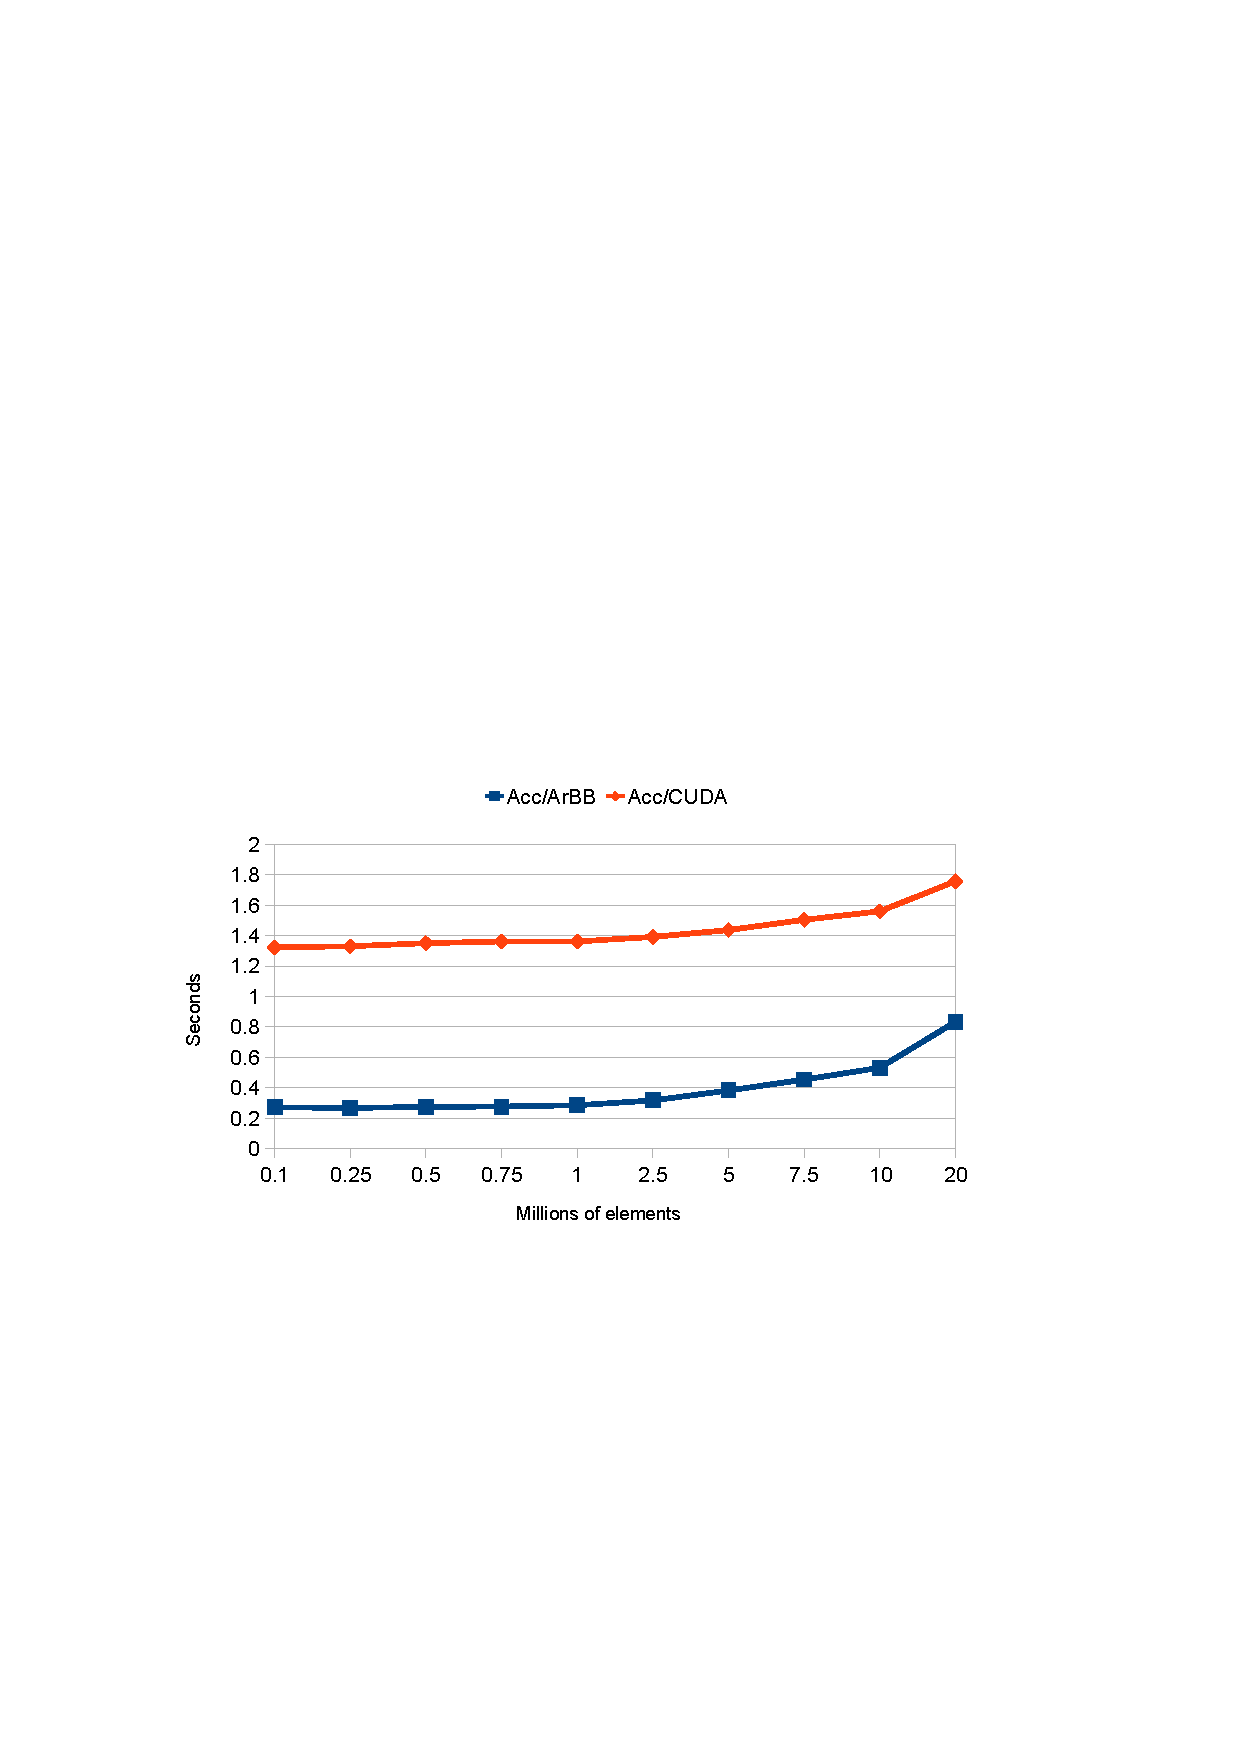
\includegraphics[width=3.5in]{./arbb/jit}    
  \end{center}
\vspace{-5mm}
  \caption{Running time experiments including JIT-time.} 
  \label{f:jit}
\end{figure}

\begin{figure}
  \begin{center}
   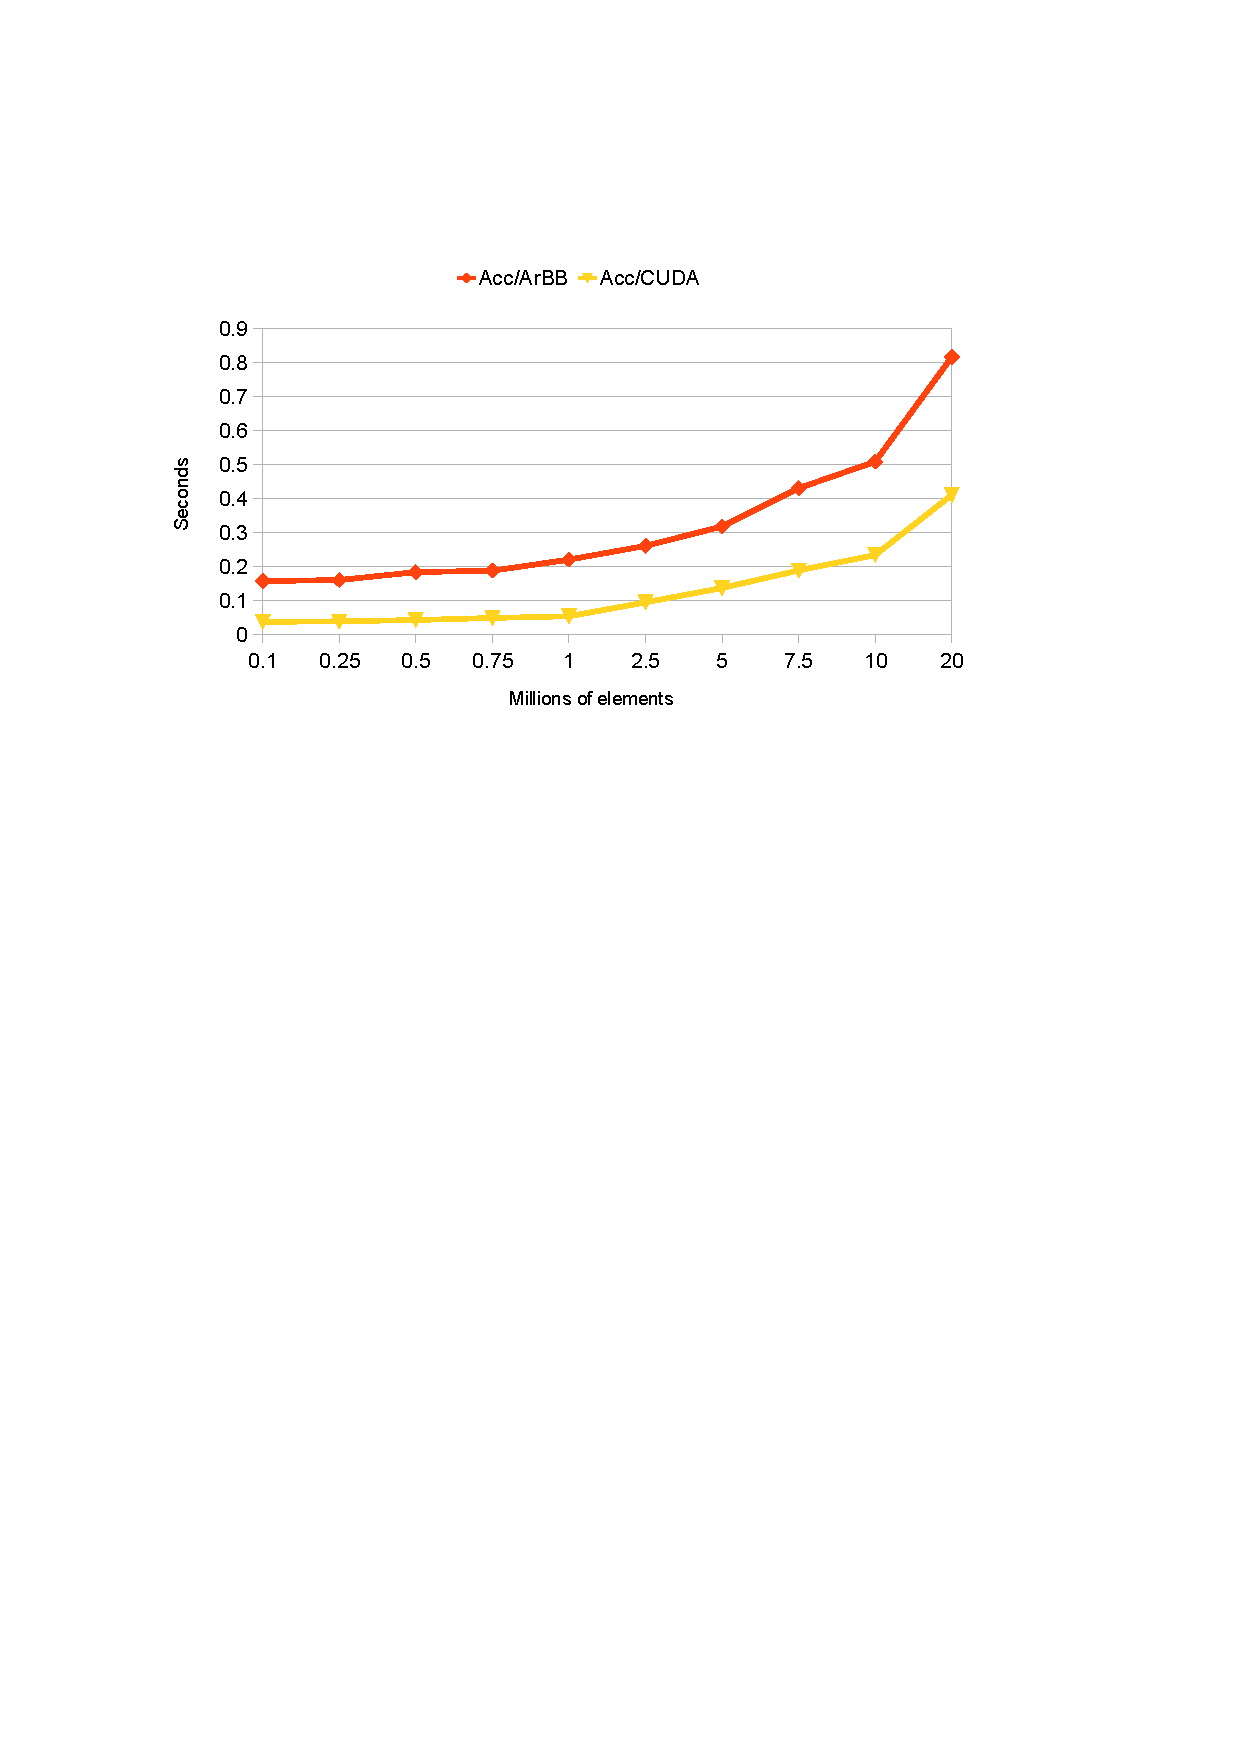
\includegraphics[width=3.5in]{./arbb/nojit}    
  \end{center}
\vspace{-5mm}
  \caption{Running time experiments JIT-time excluded.}
  \label{f:nojit}
\end{figure}


Figures~\ref{f:jit} and \ref{f:nojit} show preliminary results obtained on 
the Black-Scholes benchmark. The figures where obtained on a system with a 4-core 
Intel Core I7 975 machine with HyperThreading. The GPU used was a NVIDIA GTX480.

Figure~\ref{f:jit} shows running times obtained when JIT-time is included. 
% What this figure mainly tells us is that the JITing overhead 
JIT compilation time is much larger 
in the CUDA backend than the ArBB one.  Part of this difference 
can be attributed to the fact that 
the CUDA backend calls an external compiler (\cde{nvcc}), which takes its input in a file and runs in
a separate process.  ArBB, on the other hand, has a library interface to its  JIT-compiler. 
Figure~\ref{f:nojit} shows results obtained when pre-compiling the
CUDA functions eliminating JIT overhead.
In Accelerate, this happens automatically when the same kernel is
invoked repeatedly, because the Accelerate CUDA backed 
uses a caching scheme to avoid unnecessary JIT invocations.  (The
caching functionality has not yet been duplicated in the 
ArBB backend.)

These early results demonstrates the principle that even when a kernel
executes with higher throughput on a GPU, in a particular program it
is difficult to decide whether a computation is worth moving to a GPU,
incurring extra data-movement and possibly extra JIT compilation
\citearbb{wheres-the-data-paper}.  Specifically, we see that the
Accelerate Black-Scholes program from Figure~\ref{fig:blackscholes}
performs better on the CPU if it executes once (even on a large window
of data) whereas the GPU would yield better performance in a sustained
series of executions.
%
Because both CPU and GPU execution may be desirable---and the
selection may be dynamic---it is beneficial to have a single source code
that is portable across both.  
% Accelerate combined with \systemname{} makes this possible.


% ====================================================================================================
\subsection{Related Work}
% ====================================================================================================


OpenCL~\citearbb{opencl08} is a programming model very similar to CUDA but with the aspiration 
to offer both acceleration of computations on GPUs or to multicore CPUs. 
OpenCL JIT compiles the kernels for the particular hardware available and is
in that sense similar to ArBB.  
OpenCL programs are relatively low-level and require a large amount of
boilerplate to create and invoke.  In this sense they occupy a very
different niche than Accelerate.

Microsoft Accelerator~\citearbb{ACCELERATOR} is an embedded language with similar 
aspirations as ArBB, that is, to target a diverse range of architectures using the 
same source code. Accelerate can be used from the C\# language or the 
functional F\# language and targets GPUs or of CPUs and their
vector units.
% However, being part of the .Net framework implies limited accessibility 
%for platforms other than Microsoft Windows.  

\rn{What's the comparison with our stuff?}

%Most work on partitioning workloads between 
Many CPU and GPU comparisons, and some CPU/GPU workload partitioners \citearbb{merge}, rely on
redundant hand-written versions of all kernels
% \citearbb{cpu-gpu-partitioning} 
(though some systems like Qilin \citearbb{qilin} allow a single source code).
It is difficult in this kind of scenario
to make fair comparisons, controlling for the
amount of effort put into the respective implementations.
For example, comparing unoptimized serial CPU implementations vs. GPU
ones is not informative \citearbb{debunking-dubey}.
In \systemname{} controlling for effort
need happen only once---both CUDA and ArBB are
independently optimized by their respective teams of engineers---not for each benchmark.


% ====================================================================================================
% \section{Future work and Conclusions}
%\section{Future Work}
% ====================================================================================================

%\rn{need to be careful about being too repetitive...}
%The \accarbb{} backend is currently work-in-progress. The Accelerate
%functionality is not yet completely covered by the ArBB backend. Currently 
%the ArBB back-ed is operational for Accelerate programs using {\em Map}, 
%{\em ZipWith} and some simple instances of the Accelerate {\em Fold} operation.
%All of these also have the limitation that they only work for up to and 
%including 3-dimensional arrays using the ArBB backend while the Accelerate
%model allows the N-dimensional case. Allowing the N-dimensional case 
%in the ArBB backend for the supported operations range from a simple exercise 
%to more intricate problems needing some thought. For example, in the case 
%{\em Map} operations the needed transformation is simple (Accelerate Maps 
%over N-dimensional arrays is a per-element operation). One could flatten 
%the N-dimensional array to a 1-dimensional array (remembering its old shape) 
%perform the map and then transform the array back into N-dimensions. In 
%the case of {\em Fold} (reductions) the situation becomes more tricky. 
%transforming the arrays to arrays of lesser dimensionality then requires 
%a so-called segmented {\em Fold} operation. 

%The current \accarbb{} backend uses a hybrid of immediate-mode 
%and retained-mode programming styles. Moving more towards 
%retained-mode only may have performance benefits since it would give the 
%ArBB compiler larger programs to optimize. Exploring this aspect is left 
%as future work. 

% ====================================================================================================
\subsection{Discussion and Conclusions}
% ====================================================================================================

We have demonstrated that an EDSL such as Accelerate is sufficiently
platform-independent to break free of its original hardware target
(CUDA/GPU) and create efficient programs on other architectures.  This
gives us hope that \systemname{}/Accelerate programs will be
forward-portable to future parallel architectures and instruction
sets.

The EDSL approach changes the playing field for the designer
of compiler backends.  Rather than contending with full blown
languages and their complexities (e.g. pointers, aliasing,
inheritance, virtual functions, etc), compiler backends can focus on
simple value-oriented compute languages.

%% Achieving the ultimate goal of performance portability requires
%% progress on two research problems.  The first is EDSLs themselves and
%% their integration into host languages.  The second problem 

But the EDSL method solves only part of the performance-portability problem.
Simple as EDSL target languages may be, there remains a
substantial challenge in mapping them efficiently to the diversity
of parallel architectures available now and in the near future.
%especially without requiring a large amount of additional per-platform
%user annotations.
\textred{For example, the idiosyncrasies of memory bank access on
  NVIDIA GPUs must be taken into account to generate efficient
  implementations of the high-level collective operations that we have
  discussed.}

This is a compiler backend research challenge.
The {\em skeletons} method mentioned in
Section~\ref{sec:accelerate-arbb} is one approach to this problem, as
are the optimizations studied in the Copperhead \citearbb{copperhead} and
Obsidian \citearbb{JSLIC} projects.
%
On the other hand, systems that rely on advanced optimizations
typically suffer to some extent from performance-predictability
problems.  Thus achieving portable, predictable performance on a wide range
of architectures---even for the simplest target languages---will
be the subject of much future work.

%{
%\small
\bibliographystylearbb{alpha}
\bibliographyarbb{thesis}
%}


%\end{document}





\cleardoublepage


% ---------------------------------------------------------------------------
% nocites 
% ---------------------------------------------------------------------------
%% \nocite{*}



%% \makeatletter
%% \renewenvironment{thebibliography}[1]
%%      {\chapter*{\bibname}%
%%       \@mkboth{\MakeUppercase\bibname}{\MakeUppercase\bibname}%
%%       \list{\@biblabel{\@arabic\c@enumiv}}%
%%            {\settowidth\labelwidth{\@biblabel{#1}}%
%%             \leftmargin\labelwidth
%%             \advance\leftmargin\labelsep
%%             \@openbib@code
%%             \usecounter{enumiv}%
%%             \let\p@enumiv\@empty
%%             \renewcommand\theenumiv{\@arabic\c@enumiv}}%
%%       \sloppy
%%       \clubpenalty4000
%%       \@clubpenalty \clubpenalty
%%       \widowpenalty4000%
%%       \sfcode`\.\@m}
%%      {\def\@noitemerr
%%        {\@latex@warning{Empty `thebibliography' environment}}%
%%        \endlist}
%% \makeatother

%% \bibliographystyle{alpha}
%% \bibliography{thesis}
%% \addcontentsline{toc}{chapter}{Bibliography}

\end{document}
